\emph{\textbf{Химическая технология}}

\textbf{Қазанқапова М.Қ., Ермағамбет Б.Т., Қожамұратова Ұ.М.,
Малғаждарова А.Б.}

\emph{PRODUCTION OF COMPOSITE CARBON ADSORBENTS BASED ON TEXTILE CORD
OBTAINED FROM CAR TIRE
RESIDUES}..................................................................................................................

\textbf{Нұрмағанбетов Ж.С., Нүркенов О.А., Фазылов С.Д ,. Ибрайбекова
А.М., Хабдолда Г.,}

\textbf{Әшірбекова Б.}

\emph{ЛУПИНИН АЗИДІНІҢ ОРЫНБАСЫЛҒАН АРИЛАЦЕТИЛЕНДЕРМЕН ӨЗАРА
ӘРЕКЕТТЕСУЛЕРІ...............................................................................................................................}

\textbf{Рожкова O.В, Ибраимова Д.M-K., Рожков В.И., Ермеков М.Т.,
Кудайбергенова С.Ж.}

\textbf{Букеева А.Б., Нуртай Ж.Т.}

\emph{Способ получения СУПЕРГИДРОФОБНОЙ ГЛИНЫ месторождения}

\emph{«Таганское» для производства БУРОВЫХ РАСТВОРОВ}

\textbf{Нургалиев Н.У., Искакова Ж.Б., Колпек А., Айбульдинов Е.К.,
Сабитов А.С., Копишев Э.Е.,}

\textbf{Салихов Р.М., Петров М.С., Алжанова Г.Ж., Абдиюсупов Г.Г.,
Өмірзақ М.Т.}

\emph{CОВМЕСТНЫЙ ПИРОЛИЗ НИЗКОСОРТНОГО ТОПЛИВА И ПРИРОДНОГО
БИТУМА\ldots\ldots\ldots\ldots..}

\textbf{Нечипуренко С.В., Канаев Р.К, Ефремов С.А., Кузнецов А.А., Мун
Г.А.} \emph{КОНЦЕНТРИРОВАНИЕ И ИССЛЕДОВАНИЕ ПРОДУКТОВ УГЛИСТЫХ СЛАНЦЕВ
МЕСТОРОЖДЕНИЯ
БАЛА-САУСКАНДЫК.............................................................................................}

\textbf{Рожкова О.В., Мұздыбаева Ш.А.,Бөкеева А.Б., Құдайбергенова С.Ж.,
Рожков В.И.,}

\textbf{Ермеков М.Т., Нұртай Ж.Т.}

\emph{БЕНТОНИТ САЗЫН ТАУ-КЕН ӨНДІРІСІНІҢ ШАХТА СУЛАРЫН ТАЗАРТУДАҒЫ
ҚОЛДАНУ ТИІМДІЛІГІ
.................................................................................................................................................}

\textbf{Dauletzhanova Zh.T.,} \textbf{Nurtaı} \textbf{Zh.T.}

\emph{RESEARCH ON COALS AND ASH RESIDUES FOR THE PRESENCE OF RARE EARTH
METALS\ldots\ldots.}

\textbf{Amankeldin D.Zh., Nurgaliyev N.U., Zhunussova E.B., Omarov
Kh.B., Zhumabekova A.K.,\\
Ussenkulova Sh.Zh., Orynbassar O.R.}

\emph{OPTIMIZATION OF THE OPERATION OF AN ISOMERIZATION INSTALLATION FOR
LIGHT PETROL
FRACTIONS\ldots\ldots\ldots\ldots\ldots\ldots\ldots\ldots\ldots\ldots\ldots\ldots\ldots\ldots\ldots\ldots\ldots\ldots\ldots\ldots\ldots\ldots\ldots\ldots\ldots\ldots\ldots\ldots\ldots\ldots\ldots\ldots\ldots\ldots\ldots\ldots\ldots.}

\textbf{Кусепова Л.А., Суюндикова Ф.О.}

\emph{ИК СПЕКТРОСКОПИЧЕСКОЕ И КВАНТОВО-ХИМИЧЕСКОЕ ИССЛЕДОВАНИЕ
СОЕДИНЕНИЙ АМИДОВ И ТИОАМИДОВ С СОЛЯНОЙ И ГЕКСАФТОРКРЕМНИЕВОЙ КИСЛОТАМИ
И СОЛЯМИ МЕДИ
(II)\ldots\ldots\ldots\ldots\ldots\ldots\ldots\ldots\ldots\ldots\ldots\ldots\ldots\ldots\ldots\ldots\ldots\ldots\ldots\ldots\ldots\ldots\ldots\ldots\ldots\ldots\ldots\ldots.}

\textbf{Nurgaliyev N.U,Aibuldinov Ye.K., Iskakova Zh.B., Kolpek A.,
Mashan T.T.,}

\textbf{Kusepova L.A., Kopishev E.Ye}

\emph{INVESTIGATION OF THE KINETICS OF THE COAL PYROLYSIS
PROCESS\ldots\ldots\ldots\ldots\ldots\ldots\ldots\ldots\ldots\ldots.}

\textbf{Romanov V.I., Merkulov V.V., Kabiyeva S.K., Bestembek E.S.,
Zhaslan R.K.,}

\textbf{Zhumanazarova G.M.}

\emph{INVESTIGATION OF THE CHEMICAL AND MINERALOGICAL COMPOSITION OF
METALLURGICAL SLAGS OF JSC ``QARMET''
TEMIRTAU\ldots\ldots\ldots\ldots\ldots\ldots\ldots\ldots\ldots\ldots\ldots\ldots\ldots\ldots\ldots\ldots\ldots\ldots\ldots{}}

\textbf{Kazankapova M.K., Yermagambet B.T., Dauletzhanova Zh.T.,Kalenova
A.M}

\emph{OBTAINING POROUS CARBON MATERIAL AND INVESTIGATION OF ITS PHYSICAL
AND CHEMICAL PROPERTIES}

\textbf{Tastanova L.K, Apendina A.K., Orynbasar R.O, Zhanserikov N.Zh.,
Nurlybay S.A.}

\emph{STUDY OF THE EFFECTIVENESS OF THE DEMULSIFIER COMPOSITION ON THE
DESTRUCTION OF LOCAL OIL-WATER
EMULSION\ldots\ldots\ldots\ldots\ldots\ldots\ldots\ldots\ldots\ldots\ldots\ldots\ldots\ldots\ldots\ldots\ldots\ldots\ldots\ldots\ldots\ldots.}

\textbf{Popov A.Y.}

\emph{PRODUCTION OF SYNTHETIC HYDROCARBONS USING COBALT CATALYSTS BASED
ON ZSM-5
ZEOLITE\ldots\ldots\ldots\ldots\ldots\ldots\ldots\ldots\ldots\ldots\ldots\ldots\ldots\ldots\ldots\ldots\ldots\ldots\ldots\ldots\ldots\ldots\ldots\ldots\ldots\ldots\ldots\ldots\ldots\ldots\ldots\ldots\ldots\ldots\ldots\ldots{}}

\textbf{Жантасов К.Т., Зият А.Ж., Якубова Р.Р., Жантасов М.К., Сакыбаев
Б.А.}

\emph{ИССЛЕДОВАНИЯ И РЕАЛИЗАЦИЯ ТЕХНОЛОГИИ ПОЛУЧЕНИЯ ОРГАНОМИНЕРАЛЬНОГО
УДОБРЕНИЯ --
ТУКОСМЕСИ\ldots\ldots\ldots\ldots\ldots\ldots\ldots\ldots\ldots\ldots\ldots\ldots\ldots\ldots\ldots\ldots\ldots\ldots\ldots\ldots\ldots\ldots\ldots\ldots\ldots\ldots\ldots\ldots\ldots\ldots\ldots\ldots..}

\emph{\textbf{Химическая технология}}

IRSTI 31.21.01

\textbf{PRODUCTION OF COMPOSITE CARBON ADSORBENTS BASED ON TEXTILE CORD
OBTAINED FROM CAR TIRE RESIDUES}

\textbf{M.K. Kazankapova, B.T. Yermagambet, U.M.Kozhamuratova, A.B.
Malgazhdarova}

«Institute of Coal Chemistry and Technology» LLP, Astana, Kazakhstan

Corresponding author: coaltech@bk.ru

Carbon chemistry opens up very wide prospects in obtaining compositions
based on carbon-containing raw materials, due to the achievements of
recent years in this field. Due to their unique properties, extremely
high chemical resistance, thermal resistance, heat resistance and
specific strength, carbon materials have found application for the
manufacture of carbon-containing refractory, high-temperature composite
materials, modified electrodes as fillers for the tire and rubber
industry, catalytic systems based on carbon-containing raw materials,
etc. Frequently used carbon materials do not meet the requirements of
the technological process, in some cases their use is economically
unjustified, since they are expensive and have a small raw material
base. Therefore, obtaining new efficient and cheap natural carbon
materials from available types of industrial raw materials is one of the
urgent tasks currently facing scientists and technologists. Textile
wire, a product of processing rubber organic waste, can become a
promising new raw material for the production of carbon-containing
materials. Porous carbon materials were obtained in a laboratory
installation, optimal parameters were determined, and the
physico-chemical properties of the feedstock and the obtained adsorbents
(ash content, humidity, volatility, density, sumar pore volume,
elemental composition) were studied.

\textbf{Key words:} textile cord, tire waste, adsorbent, porous carbon
nanomaterials.

\textbf{АВТОМОБИЛЬ ШИНАЛАРЫНЫҢ ҚАЛДЫҚТАРЫНАН АЛЫНҒАН ТОҚЫМА СЫМЫНА
НЕГІЗДЕЛГЕН КОМПОЗИТТІК КӨМІРТЕКТІ АДСОРБЕНТТЕРДІ АЛУ}

\textbf{М.Қ. Қазанқапова, Б.Т. Ермағамбет, Ұ.М. Қожамұратова, А.Б.
Малғаждарова}

«Көмір химиясы және технология институты» ЖШС, Астана, Қазақстан,

е-mail: coaltech@bk.ru

Көміртек химиясы осы саладағы соңғы жылдардағы жетістіктерге байланысты
құрамында көміртегі бар шикізат негізінде композиция алудың кең
перспективаларын ашады. Бірегей қасиеттеріне, өте жоғары химиялық
төзімділігіне, ыстыққа төзімділігіне және меншікті беріктігіне
байланысты көміртекті материалдар құрамында көміртегі бар отқа төзімді,
жоғары температуралы композициялық материалдар, модификацияланған
электродтар, шина және резеңке өнеркәсібі үшін толтырғыштар, құрамында
көміртегі бар шикізат негізіндегі каталитикалық жүйелер және т. б. Жиі
қолданылатын көміртекті материалдар технологиялық процестің талаптарына
сәйкес келмейді, кейбір жағдайларда оларды пайдалану экономикалық
тұрғыдан негізсіз, өйткені олар қымбат және шикізат базасы аз.
Сондықтан, өнеркәсіптік шикізаттың қолжетімді түрлерінен жаңа тиімді
және арзан табиғи көміртекті материалдарды алу қазіргі уақытта ғалымдар
мен технологтардың алдында тұрған өзекті міндеттердің бірі болып
табылады. Құрамында көміртегі бар материалдарды алу үшін жаңа
перспективалы шикізат тоқыма сымы-резеңке органикалық қалдықтарды қайта
өңдеу өнімі болуы мүмкін. Кеуекті-көміртекті материалдар зертханалық
қондырғыда алынды, оңтайлы параметрлер анықталды, бастапқы шикізат пен
алынған адсорбенттердің физика-химиялық қасиеттері (күл, ылғалдылық,
құбылмалылық, тығыздық, кеуектердің қосынды көлемі, элементтік құрамы)
зерттелді.

\textbf{Түйін сөздер:} тоқыма сымы, шина қалдықтары, адсорбент, кеуекті
көміртекті наноматериалдар.

\textbf{ПОЛУЧЕНИЕ КОМПОЗИТНЫХ УГЛЕРОДНЫХ АДСОРБЕНТОВ НА ОСНОВЕ
ТЕКСТИЛЬНОГО КОРДА ПОЛУЧЕННОГО ИЗ ОСТАТКОВ АВТОМОБИЛЬНЫХ ШИН}

\textbf{М.К. Казанкапова, Б.Т. Ермағамбет, У.М. Кожамуратова, А.Б.
Малгаждарова}

ТОО «Институт химии угля и технологии», Астана, Казахстан,

е-mail: coaltech@bk.ru

Химия углерода открывает весьма широкие перспективы в получении
композиции на основе углеродсодержащего сырья, в силу достижений
последних лет в этой области. Благодаря уникальным свойствам,
чрезвычайно высокой химической стойкости, термопрочности, термостойкости
и удельной прочности углеродные материалы нашли применение для
изготовления углеродсодержащих огнеупорных, высокотемпературных
композиционных материалов, модифицированных электродов, как наполнителей
для шинной и резинотехнической промышленности, каталитических систем на
основе углеродсодержащего сырья и др. Часто используемые углеродные
материалы не соответствуют требованиям технологического процесса, в
некоторых случаях их использование экономически неоправданно, так как
они дороги и имеют небольшую сырьевую базу. Поэтому, получение новых
эффективных и дешевых природных углеродных материалов из доступных видов
промышленного сырья является одной из актуальных задач, стоящих в
настоящее время перед учеными и технологами. Новым перспективным сырьем
для получения углеродсодержащих материалов может стать текстильная
проволока-продукт переработки резиновых органических отходов.
Пористо-углеродные материалы получены в лабораторной установке,
определены оптимальные параметры, изучены физико-химические свойства
исходного сырья и полученных адсорбентов (зольность, влажность,
летучесть, плотность, сумарный объем пор, элементный состав).

\textbf{Ключевые слова:} текстильный корд, отходы шин, адсорбент,
пористые углеродные наноматериалы.

\textbf{Introduction.} The environmentally acceptable management of
excess tires, which belong to the category of solid waste, and which are
discarded every year worldwide by more than three million, is a problem
worldwide {[}1{]}. The properties that make them desirable as tires,
namely durability, make their disposal and recycling difficult, since
they are almost immune to biological degradation {[}2{]}. A feature of
the application of this technology is the method of processing, without
the use of cryogenic technologies, which avoids harmful emissions into
the environment and preserves the developed and active surface of the
crushed rubber powder. With this method of tire recycling, it is
possible to ensure minimal harmful emissions, and sometimes practically
their absence {[}3{]}. The source of carbon-containing materials can be
textile cord, which are stored in landfills in sufficient quantities for
their industrial use. Taking into account the complex chemical
compositions of carbon-containing raw materials, obtaining products of
specified properties and composition becomes an urgent task of both
theoretical and practical importance {[}4{]}. Many years of tire
operation experience shows that the quality of the cord has a decisive
influence on the technical resource, maintainability and other quality
indicators. The cord in the tire works in harsh conditions, being
subjected to a variety of static and dynamic stresses, multiple strains
of stretching, compression, bending, torsion, etc.The following brands
of cords are produced by the industry: viscose, nylon, anide, acid,
polyester, glass cord, metal cord {[}5{]}.

Viscose cord is used in the production of tires for trucks and passenger
cars, motorcycles, tractors and agricultural machinery {[}6{]}.
Transitional pores are those in which capillary condensation takes
place, and macropores have such large radii that the phenomenon of
capillary condensation becomes impossible {[}7{]}. The cord threads are
positioned at a certain angle of the plane drawn through the wheel axis
{[}8{]}. Carbon burns out over the entire grain volume, which leads to
the development of a porous structure of coal with a significant
increase in the volume of micro- and transitional pores {[}9{]}. Due to
their unique properties, extremely high chemical resistance, heat
resistance, heat resistance and specific strength, carbon composites
have found wide application {[}10{]}.

Porous carbon materials are obtained by heat treatment (carbonation)
and/ or activation (using various oxidants) of carbon-containing raw
materials and have the ability to efficiently separate gas and liquid
mixtures due to the dimensional and sorption effect. Such materials are
widely used as various sorbents, catalyst carriers, nanocomposite
materials, substrates in new generation current sources (lithium-ion
batteries, supercapacitors, ionistors and fuel cells), etc.

For the first time, we have obtained nanosorbents from carbonaceous
waste -- textile cord, by the method of carbonation and steam-gas
activation. The scheme for the production of carbon materials based on
textile cord for the purification of the gas phase and wastewater is
shown in Figure 1.

\begin{figure}[H]
	\centering
	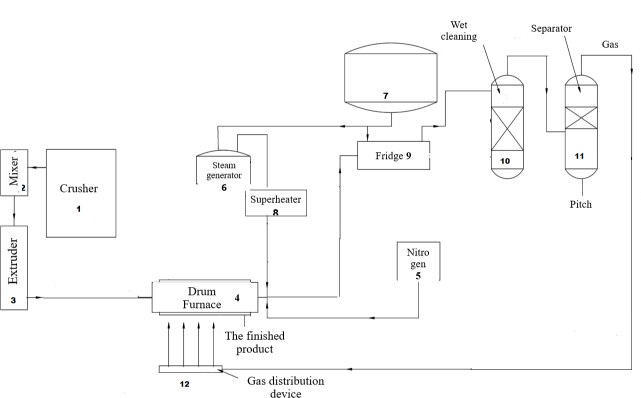
\includegraphics[width=0.8\textwidth]{assets/1004}
	\caption*{}
\end{figure}

\textbf{Figure 1 -- Technological scheme of the installation for the
production of adsorbent}

The work is aimed at developing a highly efficient technology and
creating a pilot production of carbon nanoporous materials from waste
materials. Carbon materials can be used to isolate and purify hydrogen
from synthesis gas, release nitrogen from air; purify air from methane,
monoxide and carbon dioxide; clean wastewater from toxic impurities,
manufacture supercapacitors for lithium-ion batteries and catalyst
carriers.

\textbf{Materials and methods:} The study used methods for obtaining
carbon adsorbents (carbonation and activation) in laboratory conditions,
methods for determining their physico-chemical and adsorption
properties: determination of humidity, ash content, volatility,
pH-aqueous extract, bulk density, adsorption activity by methyl orange,
method for determining the total pore volume by water, elemental
analysis, method BET for determining the specific surface area of the
obtained materials, methods of water purification from oil and iron in
laboratory conditions, methods of wastewater and gas purification from
acidic components, etc.

Instruments were used: laboratory quartz reactor, rotary tubular furnace
BR-12NRT, thermogravimetric analyzer (Thermostep Eltra), Crystallux gas
chromatograph, Shaker Incubator ES-20/60, spectrophotometer (PD-303), pH
meter, centrifuge, ultrasonic bath, muffle furnace, ultrasonic bath,
scanning electron microscopy, X-ray-fluorescent analyzer, energy
dispersion elemental analysis, etc.

\textbf{Results:} The technological process was carried out in two
stages: carbonation (700°C) (to remove volatile components and obtain a
large-porous structure evenly distributed throughout the volume) and
activation (800°C) (to obtain a microporous structure). The experiments
were carried out on a laboratory installation of steam and gas
activation

A drawing of the laboratory reactor is shown in Figure 2.

\begin{figure}[H]
	\centering
	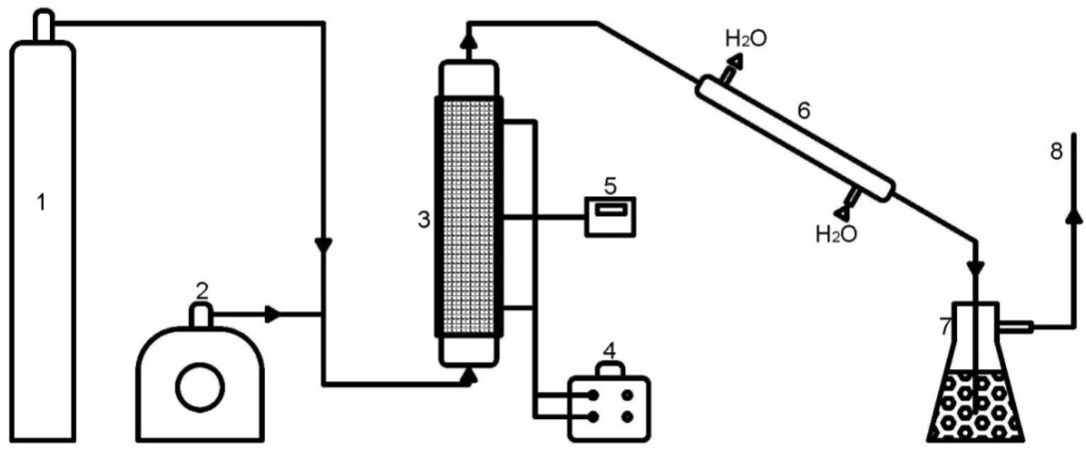
\includegraphics[width=0.8\textwidth]{assets/1005}
	\caption*{}
\end{figure}

\textbf{Figure 2 -- Schematic diagram of a laboratory installation of
steam and gas activation:} \emph{1 -- gas cylinder (argon); 2 -- steam
generator; 3 -- reactor; 4 -- LATR; 5 -- thermal sensor; 6 -- direct
refrigerator; 7 -- flask for gas purification from resins; 8 -- gas
outlet}

Carbonation was carried out in an inert argon medium in the temperature
range of 400-800 C for 60 minutes. Argon was supplied from a cylinder
(1) to a reactor with a predetermined flow rate of 20 ml/min, which was
installed using a flow meter. After the reactor, the gas was sent to the
refrigerator (6), from where part of the condensed gas was poured into
the flask (7) for purification from resinous substances. The unreacted
gases were discharged into the ventilation system (8).

At the next stage of preparation of the adsorbent, to improve its
adsorption properties, activation with water vapor (consumption 10
ml/min) was carried out at a maximum temperature with an exposure time
of 60 minutes.

Table 1 shows the temperature dependences of the components of the gas
obtained as a result of carbonation and activation of the nylon cord.
The formation of combustible gas components (CO, H\textsubscript{2},
CH\textsubscript{4}) occurs in accordance with the basic chemical
reactions:

2H\textsubscript{2}O → 2H\textsubscript{2} + O\textsubscript{2} --
115700 kkal (1)

C + H\textsubscript{2}O → CO + H\textsubscript{2} -- 28150 kkal (2)

C + CO\textsubscript{2} → 2CO -- 38400 kkal (3)

C + 2H\textsubscript{2} → CH\textsubscript{4} + 18600 kkal (4)

Textile cord under heat treatment above 200°C begins to decompose to
form a combustible gas, which contains hydrogen, carbon monoxide,
alkanes and alkenes.

\textbf{Table 1 -- Gas composition of carbonation and activation of
textile cord}

\begin{longtable}[]{@{}
  >{\raggedright\arraybackslash}p{(\columnwidth - 20\tabcolsep) * \real{0.1133}}
  >{\raggedright\arraybackslash}p{(\columnwidth - 20\tabcolsep) * \real{0.0740}}
  >{\raggedright\arraybackslash}p{(\columnwidth - 20\tabcolsep) * \real{0.0903}}
  >{\raggedright\arraybackslash}p{(\columnwidth - 20\tabcolsep) * \real{0.0902}}
  >{\raggedright\arraybackslash}p{(\columnwidth - 20\tabcolsep) * \real{0.0753}}
  >{\raggedright\arraybackslash}p{(\columnwidth - 20\tabcolsep) * \real{0.0903}}
  >{\raggedright\arraybackslash}p{(\columnwidth - 20\tabcolsep) * \real{0.0902}}
  >{\raggedright\arraybackslash}p{(\columnwidth - 20\tabcolsep) * \real{0.0753}}
  >{\raggedright\arraybackslash}p{(\columnwidth - 20\tabcolsep) * \real{0.0902}}
  >{\raggedright\arraybackslash}p{(\columnwidth - 20\tabcolsep) * \real{0.0903}}
  >{\raggedright\arraybackslash}p{(\columnwidth - 20\tabcolsep) * \real{0.1204}}@{}}
\toprule\noalign{}
\multirow{2}{*}{\begin{minipage}[b]{\linewidth}\raggedright
Process
\end{minipage}} &
\multirow{2}{*}{\begin{minipage}[b]{\linewidth}\raggedright
Т\textsubscript{1},°C
\end{minipage}} & \multicolumn{9}{l@{}}{%
\begin{minipage}[b]{\linewidth}\raggedright
Composition of gases about, \%
\end{minipage}} \\
& & \begin{minipage}[b]{\linewidth}\raggedright
О\textsubscript{2}
\end{minipage} & \begin{minipage}[b]{\linewidth}\raggedright
H\textsubscript{2}
\end{minipage} & \begin{minipage}[b]{\linewidth}\raggedright
CO\textsubscript{2}
\end{minipage} & \begin{minipage}[b]{\linewidth}\raggedright
N\textsubscript{2}
\end{minipage} & \begin{minipage}[b]{\linewidth}\raggedright
CH\textsubscript{4}
\end{minipage} & \begin{minipage}[b]{\linewidth}\raggedright
CO
\end{minipage} & \begin{minipage}[b]{\linewidth}\raggedright
Ethane
\end{minipage} & \begin{minipage}[b]{\linewidth}\raggedright
Ethylene
\end{minipage} & \begin{minipage}[b]{\linewidth}\raggedright
Propane + Propylene
\end{minipage} \\
\midrule\noalign{}
\endhead
\bottomrule\noalign{}
\endlastfoot
\multirow{5}{*}{Carbonation} & 200 & 37.003 & 0.046 & 0.126 & 32.911 &
0.166 & 0.040 & 0.005 & - & 0.589 \\
& 300 & 37.874 & 0.259 & 1.139 & 68.089 & 0.083 & - & 0.009 & 0.335 &
0.020 \\
& 400 & 43.355 & 0.237 & 2.219 & 66.944 & 0.045 & - & 0.036 & 0.680 &
0.054 \\
& 500 & 34.788 & 3.380 & 1.874 & 58.749 & 1.082 & - & 1.095 & 0.705 &
1.012 \\
& 600 & 54.526 & 10.091 & 1.671 & 36.023 & 2.570 & - & 0.918 & 0.565 &
1.012 \\
\multirow{3}{*}{Activation} & 700 & 30.469 & 3.873 & 0.411 & 76.123 &
0.746 & - & 0.137 & 0.036 & 0.162 \\
& 800 & 28.204 & 5.608 & 0.302 & 75.943 & 0.813 & 0.436 & 0.066 & 0.080
& 0.082 \\
& 800 excerpt & 27.532 & 3.304 & 0.157 & 81.477 & - & - & 0.038 & 0.058
& 0.006 \\
\end{longtable}

\textbf{Table 2 -- Material balance of carbonation and activation of
textile cord}

\begin{longtable}[]{@{}
  >{\raggedright\arraybackslash}p{(\columnwidth - 10\tabcolsep) * \real{0.0365}}
  >{\raggedright\arraybackslash}p{(\columnwidth - 10\tabcolsep) * \real{0.1626}}
  >{\raggedright\arraybackslash}p{(\columnwidth - 10\tabcolsep) * \real{0.1737}}
  >{\raggedright\arraybackslash}p{(\columnwidth - 10\tabcolsep) * \real{0.0413}}
  >{\raggedright\arraybackslash}p{(\columnwidth - 10\tabcolsep) * \real{0.3387}}
  >{\raggedright\arraybackslash}p{(\columnwidth - 10\tabcolsep) * \real{0.2471}}@{}}
\toprule\noalign{}
\begin{minipage}[b]{\linewidth}\raggedright
№
\end{minipage} & \begin{minipage}[b]{\linewidth}\raggedright
Incoming products
\end{minipage} & \begin{minipage}[b]{\linewidth}\raggedright
Content, \%
\end{minipage} & \begin{minipage}[b]{\linewidth}\raggedright
№
\end{minipage} & \begin{minipage}[b]{\linewidth}\raggedright
Outgoing products
\end{minipage} & \begin{minipage}[b]{\linewidth}\raggedright
Content, \%
\end{minipage} \\
\midrule\noalign{}
\endhead
\bottomrule\noalign{}
\endlastfoot
1 & Textile cord & 71,49 & 1 & Solid residue (adsorbent) & 22,80 \\
2 & Water (us.steam) & 28,51 & 2 & Generator gas & 67,22 \\
& Total & 100 & 3 & Liquid product (water+resin) & 9,98 \\
\multicolumn{3}{@{}l}{%
} & & Total & 100 \\
\end{longtable}

The study used methods for obtaining sorbents, methods for determining
ash content, humidity, volatility of raw materials (thermogravimetric
analysis), their physico-chemical and adsorption properties: elemental
analysis; gas chromatography; SEM (scanning electron microscopy), which
determines the total volume, density of sorbents.

\begin{figure}[H]
	\centering
	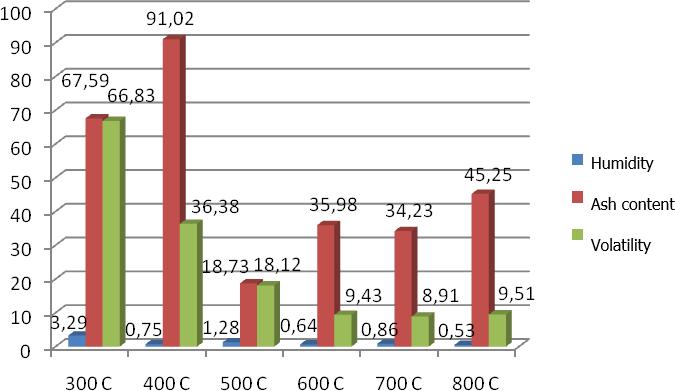
\includegraphics[width=0.8\textwidth]{assets/1006}
	\caption*{}
\end{figure}

\textbf{Figure 3 -- Results on volatility, ash content and humidity of
adsorbents from textile cord}

Based on the results of determining the total pore volume by water,
porous materials obtained at 300°C, 400°C and 800°C showed the highest
index from 5.8 to 7.9 ml/g. Therefore, this indicates a high degree of
porosity of the adsorbent.

\begin{figure}[H]
	\centering
	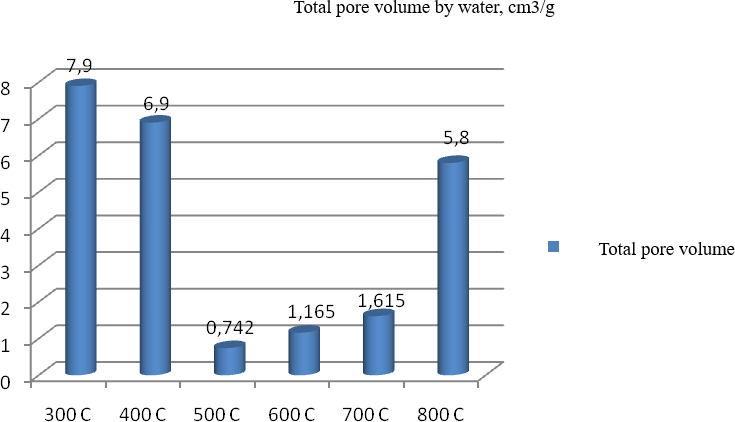
\includegraphics[width=0.8\textwidth]{assets/1007}
	\caption*{}
\end{figure}

\textbf{Figure 4 -Results of measuring the total pore volume of
adsorbents in water at different temperatures}

According to the results of determining the density of adsorbents, the
lowest density of adsorbents was shown by the initial product (0.098 g
/cm\textsuperscript{3}), also at 300°C, the value of which was 0.167 g
/cm\textsuperscript{3}. The density of all adsorbents increased compared
to the initial sample.

\begin{figure}[H]
	\centering
	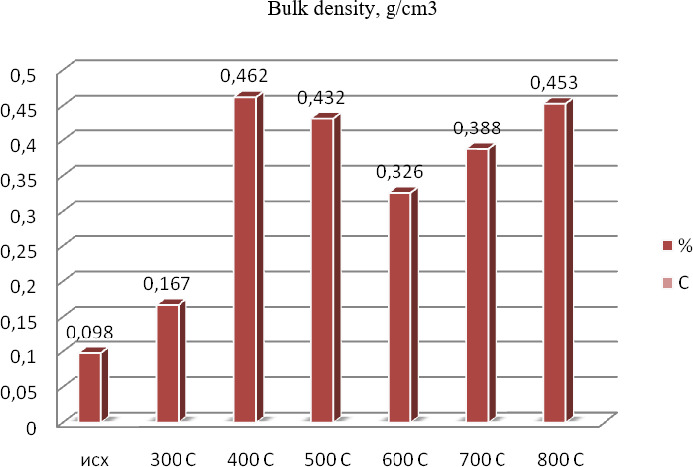
\includegraphics[width=0.8\textwidth]{assets/1008}
	\caption*{}
\end{figure}

\textbf{Figure 5 -- Bulk density of adsorbents from textile cord}

The study of the elemental composition, structure and dimension of the
samples was carried out by energy dispersive X-ray spectroscopy on a SEM
(Quanta 3D 200i) device with an energy dispersive analysis prefix from
EDAX. The energy of the exciting electron beam in the analysis was 15
keV.

The elemental composition of the initial textile cord is shown in Figure
6.

\begin{longtable}[]{@{}
  >{\raggedright\arraybackslash}p{(\columnwidth - 4\tabcolsep) * \real{0.4198}}
  >{\raggedright\arraybackslash}p{(\columnwidth - 4\tabcolsep) * \real{0.2901}}
  >{\raggedright\arraybackslash}p{(\columnwidth - 4\tabcolsep) * \real{0.2901}}@{}}
\toprule\noalign{}
\begin{minipage}[b]{\linewidth}\raggedright
Element
\end{minipage} & \begin{minipage}[b]{\linewidth}\raggedright
Wt\%
\end{minipage} & \begin{minipage}[b]{\linewidth}\raggedright
At\%
\end{minipage} \\
\midrule\noalign{}
\endhead
\bottomrule\noalign{}
\endlastfoot
C & 74.10 & 81.40 \\
O & 20.76 & 17.12 \\
Na & 0.32 & 0.18 \\
Al & 0.15 & 0.07 \\
Si & 0.29 & 0.14 \\
S & 0.60 & 0.25 \\
Ca & 0.34 & 0.11 \\
Fe & 0.90 & 0.21 \\
Cu & 0.62 & 0.13 \\
Zn & 1.91 & 0.38 \\
\end{longtable}

\begin{figure}[H]
	\centering
	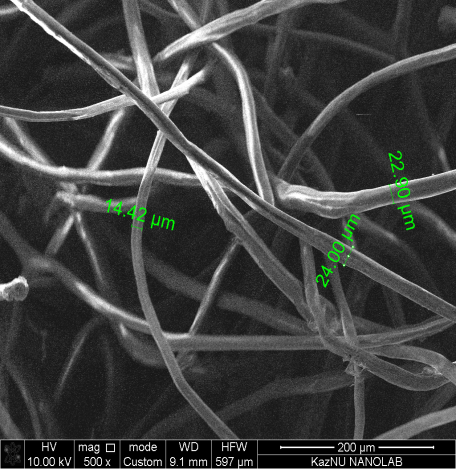
\includegraphics[width=0.8\textwidth]{assets/1009}
	\caption*{}
\end{figure}

а)

\begin{longtable}[]{@{}
  >{\raggedright\arraybackslash}p{(\columnwidth - 4\tabcolsep) * \real{0.4094}}
  >{\raggedright\arraybackslash}p{(\columnwidth - 4\tabcolsep) * \real{0.3190}}
  >{\raggedright\arraybackslash}p{(\columnwidth - 4\tabcolsep) * \real{0.2716}}@{}}
\toprule\noalign{}
\begin{minipage}[b]{\linewidth}\raggedright
Element
\end{minipage} & \begin{minipage}[b]{\linewidth}\raggedright
Wt\%
\end{minipage} & \begin{minipage}[b]{\linewidth}\raggedright
At\%
\end{minipage} \\
\midrule\noalign{}
\endhead
\bottomrule\noalign{}
\endlastfoot
C & 89.64 & 93.71 \\
O & 6.23 & 4.89 \\
Na & 0.86 & 0.47 \\
Al & 0.08 & 0.04 \\
Si & 0.20 & 0.09 \\
S & 0.29 & 0.13 \\
Ca & 0.49 & 0.19 \\
Fe & 0.05 & 0.02 \\
Cu & 0.30 & 0.09 \\
Zn & 0.32 & 0.07 \\
\end{longtable}

\begin{figure}[H]
	\centering
	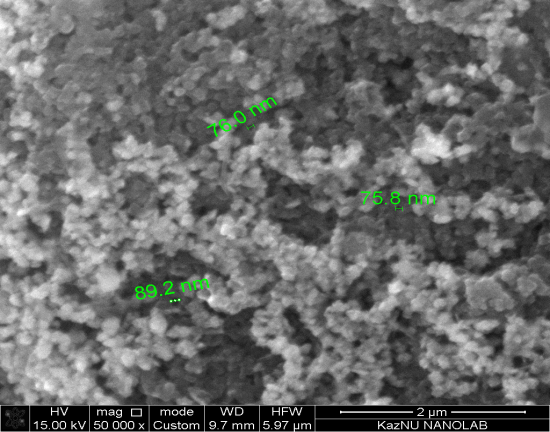
\includegraphics[width=0.8\textwidth]{assets/1010}
	\caption*{}
\end{figure}

b)

\textbf{Figure 6 - SEM images of the original (a) and activated (b)
textile cord}

In Figure 6 (a), fiber particles with a diameter of 10 to 25 microns are
clearly visible, the structural elements take the form of fibrils --
filamentous formations.

The results of the analysis of micrographs show (Fig.6 (b)) that after
heat treatment, the surface structure changes with smaller particle
sizes (up to \textasciitilde145 nm), fine carbon nanoparticles with a
diameter from 70 to 600 nm were formed, this may be due to the fact that
as a result of carbonization and activation, the forming
reactively-capable radicals interact with each other to form new
substances. The nucleation and growth of ordered carbon during the heat
treatment of textile cord can occur by self-organization of carbon
nanoparticles without the participation of mesophase, however,
additional research is required to clarify this issue.

In the laboratory of the Institute of Coal Chemistry and Technology LLP,
the obtained carbon nanoporous materials were tested to purify gases
(composition: H\textsubscript{2}S, CO, CO\textsubscript{2},
CH\textsubscript{4}, N\textsubscript{2}, H\textsubscript{2}) from
harmful substances H\textsubscript{2}S, CO\textsubscript{2},
N\textsubscript{2} to obtain mainly combustible components CO,
CH\textsubscript{4}, H\textsubscript{2}. The results of the elemental
analysis before and after gas purifications with determination of the
degree of purification are presented in Table 3.

\textbf{Table 3 -- Approbation of adsorbents from textile cord for gas
purification}

\begin{longtable}[]{@{}
  >{\raggedright\arraybackslash}p{(\columnwidth - 20\tabcolsep) * \real{0.1395}}
  >{\raggedright\arraybackslash}p{(\columnwidth - 20\tabcolsep) * \real{0.1060}}
  >{\raggedright\arraybackslash}p{(\columnwidth - 20\tabcolsep) * \real{0.1060}}
  >{\raggedright\arraybackslash}p{(\columnwidth - 20\tabcolsep) * \real{0.0910}}
  >{\raggedright\arraybackslash}p{(\columnwidth - 20\tabcolsep) * \real{0.0909}}
  >{\raggedright\arraybackslash}p{(\columnwidth - 20\tabcolsep) * \real{0.0910}}
  >{\raggedright\arraybackslash}p{(\columnwidth - 20\tabcolsep) * \real{0.0758}}
  >{\raggedright\arraybackslash}p{(\columnwidth - 20\tabcolsep) * \real{0.0757}}
  >{\raggedright\arraybackslash}p{(\columnwidth - 20\tabcolsep) * \real{0.0758}}
  >{\raggedright\arraybackslash}p{(\columnwidth - 20\tabcolsep) * \real{0.0758}}
  >{\raggedright\arraybackslash}p{(\columnwidth - 20\tabcolsep) * \real{0.0727}}@{}}
\toprule\noalign{}
\multirow{2}{*}{\begin{minipage}[b]{\linewidth}\raggedright
Name
\end{minipage}} & \multicolumn{5}{l}{%
\begin{minipage}[b]{\linewidth}\raggedright
Gas concentration \%
\end{minipage}} & \multicolumn{5}{l@{}}{%
\begin{minipage}[b]{\linewidth}\raggedright
Degree of purification, \%
\end{minipage}} \\
& \begin{minipage}[b]{\linewidth}\raggedright
H\textsubscript{2}
\end{minipage} & \begin{minipage}[b]{\linewidth}\raggedright
CO\textsubscript{2}
\end{minipage} & \begin{minipage}[b]{\linewidth}\raggedright
CH\textsubscript{4}
\end{minipage} & \begin{minipage}[b]{\linewidth}\raggedright
CO
\end{minipage} & \begin{minipage}[b]{\linewidth}\raggedright
H\textsubscript{2}S
\end{minipage} & \begin{minipage}[b]{\linewidth}\raggedright
H\textsubscript{2}
\end{minipage} & \begin{minipage}[b]{\linewidth}\raggedright
CO\textsubscript{2}
\end{minipage} & \begin{minipage}[b]{\linewidth}\raggedright
CH\textsubscript{4}
\end{minipage} & \begin{minipage}[b]{\linewidth}\raggedright
CO
\end{minipage} & \begin{minipage}[b]{\linewidth}\raggedright
H\textsubscript{2}S
\end{minipage} \\
\midrule\noalign{}
\endhead
\bottomrule\noalign{}
\endlastfoot
Crude source gas & 46,817 & 2,091 & 7,050 & 7,546 & 0,045 & - & - & - &
- & - \\
Activated Textile cord & 0,165 & 0,075 & 0,151 & 0,047 & 0,007 & 99,6 &
96,4 & 97,8 & 99,3 & 84,4 \\
\end{longtable}

\textbf{Conclusion:} Known methods of cleaning natural objects are not
always effective, and are often environmentally unsafe. The use of
organic waste for wastewater and atmospheric treatment is acceptable
from an economic and environmental point of view, but as a rule, such
materials do not have sufficiently capacious sorption properties and
therefore they need to be carbonized and activated. As a result,
sorbents with a surface different from the original mineral are obtained
and combine the useful characteristics of the starting material and
synthetic sorbents.

In the course of the work done, a laboratory installation for the
production of adsorbents was assembled, work was carried out to improve
the methodology and technology for the production of nanosorbents, with
the determination of optimal technological parameters. The
physicochemical properties of the feedstock and the obtained adsorbents
(ash content, humidity, volatility, bulk density, total pore volume,
elemental composition) were also studied. The resulting product has been
tested for gas purification. The degree of gas purification (\%) was
H\textsubscript{2}-99.6; CO\textsubscript{2}-96.4;
CH\textsubscript{4}-97.8; CO-99.3; H\textsubscript{2}S-84.4.

\emph{\textbf{Financing}.The research was carried out with the financial
support of the Science Committee of the Ministry of Science and Higher
Education of the Republic of Kazakhstan (Grant No. AR19577512.
Development of scientific and technical foundations for the production
of microporous carbon nanomaterials for the separation and storage of
hydrogen).}

\textbf{References}

1. Rezoljucija Vserossijskoj konferencii "Novaja gosudarstvennaja
jekologicheskaja politika v real\textquotesingle nom sektore
jekonomiki", 22.11.2005, Moskva, Kreml\textquotesingle{} (in Russian)

2. Tehnologija pererabotki tverdogo ostatka piroliza avtoshin v
formovannoe toplivo / Papin A.V., Ignatova A.Ju., Nevedrov A.V.,
Shikanova K.A // Polzunovskij vestnik 2015, № 2. S. 106-108. (in
Russian)

3. Shapranko D.S., Bazanov M.M. Jekologicheski bezopasnye
resursosberegajushhie tehnologii pererabotki rezinotehnicheskih izdelij,
primenjaemye v Kuzbasse / Materialy II regional\textquotesingle noj
nauchno-prakticheskoj konferencii studentov i
shkol\textquotesingle nikov «Jekologija Kuzbassa». Kemerova: KuzGTU,
2015. (in Russian)

4. Novichkov Ju. A., Petrenko T.V., Bratchun V.I. Issledovanie processa
beskislorodnogo piroliza iznoshennyh avtomobil\textquotesingle nyh shin
// Vestnik Har\textquotesingle kovskogo nacional\textquotesingle nogo
avtomobil\textquotesingle no-dorozhnogo universiteta. 2005. № 29. S.
68-70. (in Russian)

5. Frolov Ju.N. Organizacija zashhity okruzhajushhej prirodnoj sredy v
avtotransportnom komplekse // Avtomatiz. i sovrem, tehnol. -- 1997. -
№7. -- S.37-44. (in Russian)

6. Tarasevich M.R. Jelektrohimija uglerodnyh materialov. M.: Nauka,
1984. -253 s.

7. Drugov Ju.S., Rodin A.A. Jekologicheskie analizy pri razlivah nefti i
nefteproduktov.-M.: BINOM. Laboratorija znanij, 2010.- S. 6-20. (in
Russian)

8. Farmakovskij B.V., Dzhurinskij D.V.//Issledovanija processa
nanesenija pokrytij iz raznorodnyh materialov na metallicheskie
podlozhki metodom HGDN. Voprosy materialovedenija. 2003. №2 (34). (in
Russian)

9. Muhutdinov A.A., Minhajdarova G.V., Muhutdinov Je.A. Primenenie
tverdogo ostatka piroliza dlja ochistki stochnyh vod // Jekologija i
promyshlennost\textquotesingle{} Rossii. 2006 №7. S.37-41. (in Russian)

10. Vajnerman A.E., Kirilin Je.F., Rybin V.V., Chumakova I.V., Shekalov
B.I.//Problemy i dostizhenija v oblasti sozdanija mednyh splavov,
prisadochnyh materialov i tehnologii svarki i naplavki dlja izdelij
sudovogo mashinostroenija. Voprosy materialovedenija, 1999. №3 (20)-S.
241-260. (in Russian)

\emph{\textbf{Information about the authors}}

Kazankapova M.K. \textbf{-} PhD in Philosophy, assoc. professor, member
correspondent of the KazNANS, Project Manager, Leading Researcher, Head
of Laboratory of LLP "Institute of Coal Chemistry and Technology",
Astana, Kazakhstan, e-mail: maira\_1986@mail.ru;

Yermagambet B.T. - Doctor of Chemical Science, Professor, Academician of
the KazNANS, Chief Researcher, Director of LLP "Institute of Coal
Chemistry and Technology", Astana, Kazakhstan, e-mail: bake.yer@mail.ru;

Kozhamuratova U.M. \textbf{--} master student Eurasian National
University of L.N. Gumilyov\textbf{,} Astana, Kazakhstan, e-mail:
kozhamuratova.u@mail.ru;

Malgazhdarova A.B. \textbf{--} master student Eurasian National
University of L.N. Gumilyov\textbf{,} Astana, Kazakhstan, e-mail:
malgazhdarova.ab@mail.ru.

\emph{\textbf{Сведения об авторах}}

Казанкапова М.К.- PhD философских наук, асс. профессор, чл.-корр.
КазНАЕН, руководитель проекта, ведущий научный сотрудник, заведующая
лабораторией ТОО «Институт химии и технологии угля», Астана, Казахстан,
e-mail: maira\_1986@mail.ru;

Ермагамбет Б.Т. -доктор химических наук, профессор, академик КазНАЕН,
главный научный сотрудник, директор ТОО «Институт химии и технологии
угля», Астана, Казахстан, e-mail: bake.yer@mail.ru;

Кожамуратова У.М. -- магистрант Евразийского национального университета
им. Л.Н. Гумилева, Астана, Казахстан, e-mail: kozhamuratova.u@mail.ru;

Малгаждарова А.Б. -- магистрант Евразийского национального университета
им. Л.Н. Гумилева, Астана, Казахстан, e-mail: malgazhdarova.ab@mail.ru.

ҒТАМР 31.23.21

\textbf{ЛУПИНИН АЗИДІНІҢ ОРЫНБАСЫЛҒАН АРИЛАЦЕТИЛЕНДЕРМЕН}

\textbf{ӨЗАРА ӘРЕКЕТТЕСУЛЕРІ}

\textbf{Ж.С. Нұрмағанбетов\textsuperscript{1,2}, О.А.
Нүркенов\textsuperscript{1}, С.Д. Фазылов\textsuperscript{1}, А.М.
Ибрайбекова\textsuperscript{2},}

\textbf{Г. Хабдолда\textsuperscript{2}, Б.
Әшірбекова\textsuperscript{2}}

\textsuperscript{1}Қазақстан Республикасының Органикалық синтез жəне
көмір химиясы институты,

Қарағанды, Қазақстан,

\textsuperscript{2}Қарағанды медицина университеті. Қарағанды,
Қазақстан,

Корреспондент-автор: iosu8990@mail.ru

Мақалада лупинин алкалоидының екіорынбасылған 1\emph{Н}-1,2,3-үшазол
туындылары қатарының синтезі мен құрылымдық ерекшеліктері туралы
зерттеулердің нәтижелері келтірілген. Лупинин алкалоидының химиялық
трансформациясы хинолизин қаңқасының С-1 жағдайда орналасқан
гидроксиметилен тобы бойынша жүзеге асырылды. Реакциялар үш кезеңде әр
түрлі еріткіштерде жүргізілді. Лупининнің метансульфохлоридпен
үшэтиламиннің қатысуымен өзара әрекеттесуі кезінде жоғары шығымдылықпен
лупининнің мезилаты оңай түзілетіні көрсетілді. Осы қосылысты
диметилформамид ерітіндісінде натрий азидімен ары қарай қыздырып өңдеу
нәтижесінде жоғары шығыммен лупинин азидінің түзілуі жүреді. Жаңа
азидтің мыс купоросының сулы және натрий аскорбаты қатысуымен
диметилформамид ерітіндісінде әртүрлі сипаттағы функционалды
орынбасылған ароматты алкиндермен өзара әрекеттесуі кезінде оларға
сәйкес 4-алмастырылған лупининнің үшазолды туындыларының түзілуі мүмкін
екендігі анықталды. Лупининнің үшазолды циклінің негізінде С-4
жағдайында орынбасылған ароматты жаңа туындылары синтезделді.
Синтезделген үшазолдықосылыстардың құрылысы ЯМР \textsuperscript{1}Н
және \textsuperscript{13}С спектрлерін талдау негізінде дәлелденілді.
Жаңа заттардың ЯМР \textsuperscript{13}С спектрлеріндегі сигналдардың
мультиплеттілігі J-модуляция режимінде (JMOD) жазылған спектрлер бойынша
анықталды. Синтезделген қосылыстардың құрылысы сондай-ақ екі өлшемді
COSY (\textsuperscript{1}H-\textsuperscript{1}H) және HMQC
(\textsuperscript{1}H-\textsuperscript{13}C) спектрлерінің деректерімен
зерттелген. ЯМР спектрлердегі химиялық ығысулардың мәндері
\textsuperscript{1}Н және \textsuperscript{13}С сигналдарының
мультиплеттілігі және интегралды қарқындылығы бір өлшемді ЯМР
спектрлерімен анықталды.

\textbf{Түйін сөздер:} хинолизинді алкалоид, лупинин, азид, ароматты
ацетилендер, үшазолдар, 1,3-екіполярлы циклді қосылу реакциясы.

\textbf{ВЗАИМОДЕЙСТВИЕ АЗИДА ЛУПИНИНА С ЗАМЕЩЕННЫМИ АРИЛАЦЕТИЛЕНАМИ}

\textbf{Ж.С. Нурмаганбетов\textsuperscript{1,2}, О.А.
Нуркенов\textsuperscript{1}, С.Д. Фазылов\textsuperscript{1}, А.М.
Ибрайбекова\textsuperscript{2} ,}

\textbf{Г. Хабдолда\textsuperscript{1}, Б.
Аширбекова\textsuperscript{2}}

\textsuperscript{1}Институт органического синтеза и углехимии Республики
Казахстан,

Караганда, Казахстан,

\textsuperscript{2}Медицинский университет Караганды. Караганда,
Казахстан,

e-mail: iosu8990@mail.ru

В статье приведены результаты исследований по синтезу и особенностей
строения ряда новых дизамещенных 1\emph{Н}-1,2,3-триазоловых производных
алкалоида лупинина. Химическая трансформация хинолизинового остова в
строении молекулы лупинина осуществлялась по гидроксиметиленовой группе
в положении С-1. Реакции проводились в несколько стадии в среде
различных растворителей. Показано, что при взаимодействии лупинина с
метансульфохлоридом в присутствии триэтиламина в образуется новые
мезилатные производное лупинина. Последующая обработка данного
соединения действием азида натрия в среде диметилформамида при
нагревании проводит к образованию азидпроизводного лупинина с высоким
выходом. Установлено, что при реакции азида с функционально замещенными
ароматическими ацетиленами различной природы в присутствии водного
медного купороса и аскорбата натрия в диметилформамида могут быть
образованы соответствующие 4-замещенные ароматические производные
лупинина. Получены новые производные лупинина, содержащие различные
арильные заместители в положении С-4 триазольного цикла. Строение
полученных соединений установлено на основе анализа спектров ЯМР
\textsuperscript{1}Н и \textsuperscript{13}С. Мультиплетность сигналов
новых соединений в спектрах ЯМР \textsuperscript{13}С определена по
спектрам, записанным в режиме J-модуляции (JMOD). Отнесение сигналов в
спектрах триазоловых соединений проведено с привлечением различных
современных методов корреляционной спектроскопии
\textsuperscript{1}H-\textsuperscript{1}H (COSY), и
\textsuperscript{1}H-\textsuperscript{13}C (HMBC, HSQC). Определены
значения химических сдвигов, мультиплетность и интегральная
интенсивность сигналов \textsuperscript{1}Н и \textsuperscript{13}С в
одномерных спектрах ЯМР.

\textbf{Ключевые слова}: хинолизиновый алкалоид, лупинин, азид,
ароматические ацетилены, триазолы, реакция 1,3-диполярного
циклоприсоединения.

\textbf{INTERACTION OF LUPININE AZIDE WITH SUBSTITUTED ARYLACETYLENES}

\textbf{Zh.S. Nurmaganbetov\textsuperscript{1,2}, O.A.
Nurkenov\textsuperscript{1}, S.D. Fazylov\textsuperscript{1}, A.M.
Ibraybekova\textsuperscript{2},}

\textbf{G. Khabdolda\textsuperscript{2}, B.
Аshirbеkоva\textsuperscript{2}}

\textsuperscript{1}Institute of Organic Synthesis and Coal Chemistry of
the Republic of Kazakhstan,

Karaganda, Kazakhstan,

\textsuperscript{2}Medical University of Karaganda. Karaganda,
Kazakhstan,

e-mail: iosu8990@mail.ru

The article presents the results of studies on the synthesis and
structural features of a number of disubstituted
1\emph{H}-1,2,3-triazole derivatives of the lupinine alkaloid. The
chemical transformation of the quinolysin backbone in the structure of
the lupinin molecule was carried out by the hydroxymethylene group at
position C-1. The reactions were carried out in several stages in a
medium of various solvents. It has been shown that when lupinine
interacts with methanesulfochloride in the presence of triethylamine, a
mesylate derivative of lupinine is formed in methylene chloride.
Subsequent treatment of this compound by the action of sodium azide in a
dimethylformamide medium under heating leads to the formation of an
azide derivative of lupinine with a yield of 67\%. It was found that
when azide interacts with functionally substituted aromatic acetylenes
of various natures in the presence of aqueous copper sulfate and sodium
ascorbate, corresponding 4-substituted aromatic triazole derivatives of
lupinine can be formed in dimethylformamide. New 1,2,3-triazole
derivatives of lupinine, containing various aryl substituents at the C-4
position of the triazole ring, have been obtained. The structure of the
obtained compounds was established based on the analysis of the
\textsuperscript{1}H and \textsuperscript{13}C NMR spectra. Multiplicity
of signals of new compounds in the \textsuperscript{13}C NMR spectra was
determined from the spectra recorded in the J-modulation mode (JMOD).
The assignment of signals in the spectra was carried out using various
modern methods of correlation spectroscopy
\textsuperscript{1}H-\textsuperscript{1}H (COZY), and
\textsuperscript{1}H-\textsuperscript{13}C (HMBC, HSQC). The values of
chemical shifts, multiplicity and integral intensity of
\textsuperscript{1}H and \textsuperscript{13}C signals in
one-dimensional NMR spectra are determined.

\textbf{Keywords:} quinolyzine alkaloid, lupinine, azid, aromatic
acetylenes, triazoles, 1,3-dipolar cycloaddition reaction.

\textbf{Кіріспе.} Үшазолдардың 1,2,4-туындылары негізінде жаңа тиімді
дәрілік заттарды алудың синтетикалық мүмкіндіктерін соңғы жылдардағы
әдеби деректердің көздерін талдаудан байқауға болады {[}1{]}. Олардың
бірқатар туындылары медициналық тәжірибеде саңырауқұлақ инфекцияларын
(флуконазол, итраконазол, терконазол), вирустық инфекцияларды
(рибавирин, маравирок), психикалық бұзылуларды (тразодон, нефазодон,
альпразолам, триазолам, бротизолам), сүт безі қатерлі ісігін (летрозол,
анастрозол), жүрек-қан тамырлары ауруларын (тиотриазолин, кардиотрил,
трапидил) емдеуге арналған дәрі ретінде қолданылады {[}2{]}. Ғылыми
әдебиеттерде бактерияға қарсы, аналептикалық, жергілікті анестетикалық,
анальгетикалық, қабынуға қарсы, антипиретикалық, гипертензияға қарсы,
гепатопротекторлық, кардиопротекторлық, антиоксидантты, антиагрегантты
және басқа да белсенділік түрлерін көрсететін триазолдардың бірқатар
1,2,4-туындылары белгілі {[}3-5{]}.

Биологиялық белсенді үшазолдардың 1,2,4-туындыларын іздеудің тиімді
бағыты олардың жаңа реагенттермен реакцияларын зерттеу нәтижесінде
белгісіз қосылыстар қатарының пайда болуымен ерекшеленеді {[}6-8{]}.
Реагенттердің бұл түріне мысал ретінде химиялық процестердің
әртүрлілігімен ерекшеленетін хинолизидин қатарының алкалоидтарын
қарастыруға болады {[}9-11{]}. Үшазолды 1,2,4-туындылардың үш таутомерлі
түрде кездесуіне байланысты олардың табиғи құрылымдармен реакцияларын
зерттеу органикалық химия тұрғысынан да, биологиялық белсенді
қосылыстардың жаңа қатарларын синтездеу тұрғысынан да қызығушылық
тудырады. Осылайша, үшазолдардың 1,2,4-туындыларының әр түрлі
алкалоидтармен, атап айтқанда табиғи лупинин алкалоидымен реакцияларын
жүйелі түрде зерттеу, осы негізде биологиялық белсенді қосылыстардың
жаңа топтарын синтездеудің өзіндік әдістерін әзірлеу, сондай-ақ олардың
химиялық және биологиялық қасиеттерін зерттеу өзекті мәселеге жатады.

Фармакологиялық әсерге сәйкес лупинин бактерицидті, шамалы седативті
әсерді, қысқа мерзімді антигельминтикалық және гипотензивті қасиеттерді
байқатады. Оның белгілі туындыларының ішінде эфирлері ең көп зерттелген,
олар түрлі тымауларға, ісікке қарсы және гепатопротекторлық
белсенділікке ие. Бірқатар лупинин эфирлері жергілікті анестетикалық
әсерді, сондай-ақ көкжөтелге қарсы және холинестераздарға белсенділікті
көрсетті {[}12{]}. Хлорлы лупинан, күкіртті лупинан және цианды лупинан
негізінде психикалық және моторлық бұзылулардың патогенезіне қатысатын
орталық жүйке жүйесінің \emph{сигма}-рецепторлары үшін тиімді лигандалар
ретінде лупинин алкалоидының әртүрлі туындылар қатары синтезделді
{[}13-15{]}. Сондықтан лупининге және оның жаңа туындыларына деген
қызығушылық шексіз. Лупининнің құрылысын түрлендірудің аз зерттелген
және тиімді бағыттарының бірі оның ықтимал биобелсенді үшазолды
туындыларын алу болып табылады. Осылайша, лупинин алкалоидының ықтимал
биобелсенді үшазол туындыларын түрлендірудің ыңғайлы әдістерін іздестіру
және өңдеу биоорганикалық химия мен фармакологияда маңызды өзекті
мәселенің бірі деп атауға болады.

\textbf{Материалдар және әдістер.} Жаңа заттардың ИҚ спектрлері
Vector-22 фурье спектрометрінде КВг таблеткаларында жазылған. ЯМР
\textsuperscript{1}H- және \textsuperscript{13}C-спектрлері Bruker
AV-400 (400 және 101 МГц) және Bruker DRX-500 (500 және 125 МГц)
спектрометрлерінде тіркелген. Синтезделген қосылыстардың спектрлері
CDCl\textsubscript{3} жазылды, оның қалдық сигналдары
(δ\textsubscript{С}=76.9 м.ү.) және (δ\textsubscript{Н}=7.24 м.ү.) ішкі
стандарт ретінде пайдаланылды. Алынған қосылыстардың құрылымы ЯМР
\textsuperscript{1}Н- және \textsuperscript{13}С-спектрлерін талдау
негізінде дәлелденілді, ЯМР \textsuperscript{13}С-спектрлеріндегі
сигналдардың мультиплеттілігі J-модуляция режимінде (JMOD) жазылған
спектрлер бойынша анықталды. Хинолизин қанқасы үшін
\textsuperscript{1}H-\textsuperscript{1}H (COSY) және
\textsuperscript{1}H-\textsuperscript{13}C (HMBC, HSQC) спектрлердегі
сигналдардың ерекшеліктері әр түрлі корреляциялық спектроскопиядағы
әдеби деректерді пайдалану арқылы жүзеге асырылды. Спектрлерді сараптау
кезінде келтірілген негізгі атомдардың нөмірленуі липинин молекуласының
(\textbf{1)} құрылымы бойынша қолданылды. Меншікті айналу мәндері PolAAr
3005 поляриметрінде түсірілді. Жоғары ажыратымдылықтағы масс-спектрлер
DFS ThermoScientific масс-спектрометрінде жазылған (буландырғыш
температурасы 200-250°С, ЭУ иондануы, 70 эВ). Балқу температурасы
Mettler Toledo FP900 терможүйесінде анықталды. Реакциялардың жүру
барысын бақылау Sorbfil UV-254 пластиналарында жұқақабатты хроматография
(ЖҚХ) әдісімен әртүрлі жүйелерді қолдана отырып жүзеге асырылады:
трихлорметан, трихлорметан-этил спирті, 10:1. Жұқа қабатты
хроматографияның көрінісі йод камерасында және ультракүлгін сәуледе
бақыланды. Реакция өнімдері қайта кристалдану немесе Acros силикагелінде
(0.035--0.240 мм) бағаналы хроматография арқылы таза түрде бөлінген,
элюенті еріткіштер ретінде: трихлорметан; трихлорметан-этил спирті,
100:1→10:1) қолданылды.

\textbf{Функционалды орынбасылған үшазолдардың 5a-f синтезі (жалпы
әдіс).} 6 мл ДМФА еріткішінде 0.29 г (1.5 ммоль) лупининнің азиді
\textbf{3} ерітіліп, функционалды орынбасылған ароматты ацетилендердің
\textbf{4а-f} 1.35 ммоль, мыс купоросы 0.034 г (0.135 ммоль) және
натрийдің аскорбаты 0.026 г (0.135 ммоль) қосылып 75°С температурада
қыздыру жағдайында 6-8 сағат араластырылды (реакция жүру барысы ЖҚХ
әдісімен бақыланды). Салқындату жағдайында түзілген тұнба сүзіліп
алынды, содан кейін гексан еріткішімен жуылып, кептіріліп, \textbf{5а-f}
үшазолдары алынды. Түзілген \textbf{5а-f} үшазолдар препаративті таза
алу мақсатында флеш бағанасында силикагель сорбентімен
хроматографияланды (элюент: трихлорметан, трихлорметан:этил спирті,
100:1→10:1).

\textbf{(1\emph{S},9a\emph{R})-1-{[}4-Фенил-1\emph{Н}-1,2,3-үшазол-1-ил)метил{]}октагидро-1\emph{Н}-хинолизин
5а.}

Шығымы 0.3 г (75\%). Ақ ұнтақты зат, балқу т. 196-197°С.
{[}α{]}\textsubscript{D}-19.7 (\emph{с} 0.8, трихлорметан).

ИҚ спектр (KBr), ν, см\textsuperscript{-1}: 694, 766, 835, 1441, 1466,
1485, 1505, 1612, 3120 (С=С, С=N), 2763, 2804 (хинолизидинді сақина).

ЯМР \textsuperscript{1}Н спектрі (400 МГц, CDCl\textsubscript{3}), δ,
м.ү. (J, Гц): 1.17-1.40 (3Н, м., Н-2а, 2e,8a); 1.41-1.64 (5Н, м.,
Н-8е,9a,9e,3а,7а); 1.73-1.92 (2Н, м., Н-3е,7е); 1.94-2.04 (2Н, м., Н-4а,
Н-6а); 2.06-2.11 (1Н, м., Н-9а), 2.21-2.25 (1Н, м., Н-1); 2.82-2.88 (2Н,
м., Н-4е,6е); 4.55 (1Н, д.д., J=13.6, J = 5.8, Н-10); 4.62 (1Н, д.д.,
J=13.6, J=12.0, Н-10); 7.29 (1Н, т., J=7.6, Н-4ʹʹ); 7.39 (д.д., 2Н,
J=7.4, 7.6, Н-3ʹʹ, Н-5ʹʹ); 7.70 (1Н, с., Н-5ʹ), 7.80 (2Н, д., J=7.4,
Н-2ʹʹ, Н-6ʹʹ).

ЯМР \textsuperscript{13}C спектрі (125 МГц, CDCl\textsubscript{3}), δ,
м.ү.: 20.5 (С-3); 24.7 (С-7); 25.3 (С-8); 26.3 (С-2); 29.5 (С-9); 39.1
(С-1); 48.5 (С-10); 56.9 (С-4); 57.1 (С-6); 64.2 (С-9а); 120.0 (С-5ʹ);
125.6 (2С, \emph{о}-С\textsubscript{6}Н\textsubscript{5}); 127.9 (С,
\emph{р-}С\textsubscript{6}Н\textsubscript{5}); 128.7 (2С,
\emph{m}-С\textsubscript{6}Н\textsubscript{5}); 130.7 (С,
С\textsubscript{6}Н\textsubscript{5}); 147.4 (С-4ʹ).

Масс-спектр, m/z (\%): 298 (1), 297 (8), 296 (38), 152 (42), 151 (100),
150 (59), 138 (22), 137 (11), 136 (32), 116 (16), 111 (24), 110 (19), 96
(19), 83 (36), 41 (36). Табылғаны, \emph{m}/\emph{z}: 296.1995
{[}M{]}\textsuperscript{+}.
C\textsubscript{18}H\textsubscript{24}N\textsubscript{4}. Есептелгені,
\emph{m}/\emph{z}: 296.19.

\textbf{(1\emph{S},9a\emph{R})-1-\{{[}4-(4-Этилфенил)-1\emph{Н}-1,2,3-үшазол-1-ил{]}метил\}октагидро-1\emph{Н}-хинолизин
5b.}

Шығымы 0.41 г (90\%). Ақ ұнтақты зат, балқу т. 188-190°С.
{[}α{]}\textsubscript{D}-16.8 (\emph{с} 1.0, трихлорметан).

ИҚ спектр (KBr), ν, см\textsuperscript{-1}: 723, 750, 831, 1444, 1458,
1498, 1560, 3103 (С=С, С=N); 2763, 2807 (хинолизидинді сақина).

ЯМР \textsuperscript{1}Н спектрі (400 МГц, CDCl\textsubscript{3}), δ,
м.ү. (J, Гц): 1.16 (3Н, т., J=7.2, СН\textsubscript{3}); 1.19-1.40 (3Н,
м., Н-2а,2e,8a); 1.41-1.65 (5Н, м., Н-8е,9a,9e,3а,7а); 1.74-1.90 (2Н,
м., Н-3е,7е); 1.91-2.08 (2Н, м., Н-4а,6а); 2.05-2.11 (1Н, м., Н-9а),
2.21-2.26 (1H, м., Н-1); 2.65 (2Н, кв., J=7.2, CH\textsubscript{2}),
2.82-2.88 (2Н, м., Н-4е,6е); 4.54-4.65 (2Н, м., Н-10); 7.24 (2Н, д.,
J=7.8, Н-2ʹʹ, Н-6ʹʹ); 7.67 (1Н, с., Н-5ʹ); 7.73 (2Н, д., J=7.8, H-3ʹʹ,
Н-5ʹʹ).

ЯМР \textsuperscript{13}C спектрі (101 МГц, CDCl\textsubscript{3}), δ,
м.ү.: 15.6 (CH\textsubscript{3}); 20.7 (С-3); 24.9 (С-7); 25.6 (С-8);
26.3 (С-2); 28.7 (CH\textsubscript{2}Me); 29.8 (С-9); 39.2 (С-1); 48.6
(С-10); 57.1 (С-4); 57.3 (С-6); 64.4 (С-9а); 119.9 (С-5ʹ); 125.6 (С-2ʹʹ,
С-6ʹʹ); 128.2 (С-1ʹʹ); 128.3 (С-3ʹʹ, С-5ʹʹ); 144.3 (С-4ʹʹ); 147.6
(С-4ʹ).

Масс-спектрі, m/z (\%): 325 (4), 324 (17), 231 (11), 152 (19), 151 (53),
150 (32), 136 (29), 135 (28), 122 (43), 121 (74), 120 (37), 105 (71), 91
(21), 70 (100), 69 (70). Табылғаны, \emph{m}/\emph{z}: 324.2306
{[}M{]}\textsuperscript{+}.
C\textsubscript{20}H\textsubscript{28}N\textsubscript{4}. Есептелгені,
\emph{m}/\emph{z}: 324.23.

\textbf{(1\emph{R},9a\emph{S})-1-\{{[}4-(4-Фторфенил)-1\emph{Н}-1,2,3-үшазол-1-ил{]}метил\}октагидро-1\emph{Н}-хинолизин
5c.}

Шығымы 0.32 г (76\%). Ақ ұнтақты зат, балқу т. 195-198°С.
{[}α{]}\textsubscript{D}-17.5 (\emph{с} 1.0, трихлорметан).

ИҚ спектрі (KBr), ν, см\textsuperscript{-1}: 779, 815, 835 1462, 1497,
1558, 1610, 3105, 3126 (С=С, С=N); 1108, 1126, 1157, 1223 (С-F); 2765,
2808 (хинолизидинді сақина).

ЯМР \textsuperscript{1}Н спектрі (400 МГц, CDCl\textsubscript{3}), δ,
м.ү. (J, Гц): 1.18-1.40 (3Н, м., Н-2а,2e,8a); 1.40-1.64 (м., 5Н,
Н-8е,9a,9e,3а,7а); 1.72-1.90 (2Н, м., Н-3е,7е); 1.93-2.01 (2Н, м.,
Н-4а,6а); 2.05-2.08 (1Н, м., Н-9а), 2.21-2.27 (1H, м., Н-1); 2.82-2.88
(2Н, м., Н-4е,6е); 4.54 (1Н, д.д., J=13.8, J=5.6, Н-10); 4.63 (1Н, д.д.,
J=13.8, J=11.4, Н-10); 7.07 (2Н, м., Н-3ʹʹ, Н-5ʹʹ); 7.65 (1Н, с., Н-5ʹ);
7.77 (2Н, м., H-2ʹʹ, Н-6ʹʹ).

ЯМР \textsuperscript{13}C спектрі (101 МГц, CDCl\textsubscript{3}), δ,
м.ү.: 20.4 (С-3); 24.7 (С-7); 25.4 (С-8); 26.1 (С-2); 29.7 (С-9); 39.0
(С-1); 48.5 (С-10); 56.9 (С-4); 57.1 (С-6); 64.2 (С-9а); 115.6 (д.,
\textsuperscript{2}J\textsubscript{CF}=21.7, С-3ʹʹ, С-5ʹʹ); 119.8
(С-5ʹ); 126.8 (д., \textsuperscript{4}J\textsubscript{CF}=3.2, С-1ʹʹ);
127.2 (д., \textsuperscript{3}J\textsubscript{CF}=8.2, С-2ʹʹ, С-6ʹʹ);
146.5(С-4ʹ); 162.4 (д., \textsuperscript{1}J\textsubscript{CF}=247.5,
С-4ʹʹ).

Масс-спектрі, m/z (\%): 316 (1), 315 (9), 314 (44), 152 (40), 151 (100),
150 (58), 138 (18), 137 (11), 136 (38), 111 (19), 96 (15), 83 (25).
Табылғаны, \emph{m}/\emph{z}: 314.1899 {[}M{]}\textsuperscript{+}.
C\textsubscript{18}H\textsubscript{23}N\textsubscript{4}F. Есептелгені,
\emph{m}/\emph{z}: 314.19.

\textbf{(1\emph{S},9a\emph{R})-1-(\{4-{[}4-Ацетиламино-3-(этоксикарбонил)фенил{]}-1\emph{Н}-1,2,3-триазол-1-ил\}метил)октагидро-1\emph{Н}-хинолизин
5d.}

Шығымы 0.5 г (87\%). Ақ ұнтақ зат, балқу т. 157-159°С,
{[}α{]}\textsubscript{D}-9.3 (с 0.8, трихлорметан).

ИҚ спектрі (KBr), ν, см\textsuperscript{-1}: 792, 835, 1443, 1469, 1517,
1597, 3126 (С=С, С=N); 1089, 1230, 1295 (O-С-О);1680 (HN-С=О), 1707
(O-С=О), 2682, 2763, 2808 (хинолизидинді сақина), 3261 (NH).

ЯМР \textsuperscript{1}Н спектрі (400 МГц, CDCl\textsubscript{3}), δ,
м.ү. (J, Гц): 1.18-1.37 (3Н, м., Н-2а,2e,8a); 1.40 (3Н, т., J=7.2,
СН\textsubscript{3}); 1.43-1.63 (5Н, м., Н-8е,9a,9e,3а,7а); 1.73-1.92
(2Н, м., Н-3е,7е); 1.94-2.02 (2Н, м., Н-4а,6а); 2.06-2.11 (1Н, м.,
Н-9а), 2.22 (3Н, с., СН\textsubscript{3}-NH); 2.25-2.30 (1H, м., Н-1);
2.82-2.86 (2Н, м., Н-4е,6е); 4.38 (2Н, кв., J=7.2,
ОСН\textsubscript{2}); 4.57 (1Н, д.д., J=13.7, J=5.5, Н-10); 4.62 (1Н,
д.д., J=13.7, J=11.0, Н-10); 7.71 (1Н, с., Н-5ʹ); 7.86 (1Н, д.д., J=8.8,
J=2.0, Н-6ʹʹ); 8.55 (1Н, д., J=2.0, Н-2ʹʹ); 8.73 (1Н, д., J=8.8, Н-5ʹʹ);
11.13 (1Н, с., NH).

ЯМР \textsuperscript{13}C спектрі (101 МГц, CDCl\textsubscript{3}), δ,
м.ү.: 14.1 (СН\textsubscript{3}); 20.4 (С-3); 24.7 (С-7); 25.3 (С-8);
26.1 (С-2); 25.4 (NСН\textsubscript{3}); 29.6 (С-9); 39.1 (С-1); 48.6
(С-10); 56.8 (С-4); 57.1 (С-6); 61.5 (ОСН\textsubscript{2}); 64.2
(С-9а); 115.4 (С-3ʹʹ); 119.8 (С-5ʹ); 120.4 (C-5ʹʹ); 124.9 (C-1ʹʹ); 127.7
(C-2ʹʹ); 131.4 (C-6ʹʹ); 141.1 (С-4ʹʹ); 146.3 (С-4ʹ); 168.1 (C=O эфир);
168.9 (С=О амид).

Масс-спектрі, m/z (\%): 427 (2), 426 (13), 425 (44), 411 (15), 152 (44),
151 (100), 150 (56), 136 (32), 83 (21), 43 (28). Табылғаны, m/z:
425.2420 {[}M{]}\textsuperscript{+}.
C\textsubscript{23}H\textsubscript{31}N\textsubscript{5}О\textsubscript{3}.
Есептелгені, m/z: 425.24.

\textbf{(1\emph{S},9a\emph{R})-1-\{{[}4-(3,4,5-үшметоксифенил)-1\emph{H}-1,2,3-үшазол-1-ил{]}метил\}октагидро-
1\emph{H}-хинолизин 5e.}

Шығымы 0.2 г (72\%). Ақ кристалдар, балқу т. 143-145°С.
{[}α{]}\textsubscript{D}-13.6 (\emph{с} 1.6, трихлорметан).

ИҚ спектрі (KBr), ν, см\textsuperscript{-1}: 779, 827, 860, 1467, 1500,
1585, 1639, 3110 (С=С, С=N); 1006, 1099, 1128, 1234 (С-О); 2736, 2765,
2798 (хинолизидинді сақина).

ЯМР \textsuperscript{1}Н спектрі (400 МГц, CDCl\textsubscript{3}), δ,
м.ү. (\emph{J}, Гц): 1.21-1.39 (3Н, м.,
Н-2\emph{а},2\emph{e},8\emph{a}); 1.43-1.64 (5Н, м.,
Н-8\emph{е},9\emph{a},9\emph{e},3\emph{а},7\emph{а}); 1.74-1.90 (2Н, м.,
Н-3\emph{е},7\emph{е}); 1.95-2.09 (2Н, м., Н-4\emph{а},6\emph{а});
2.12-2.17 (1Н, м., Н-9\emph{а}), 2.29-2.34 (1H, м., Н-1); 2.79-2.94 (2Н,
м., Н-4\emph{е},6\emph{е}); 3.84 (C-4ʹʹ тегі 3Н, с.,
OСН\textsubscript{3}); 3.91 (C-3ʹʹ, С-5ʹʹ тегі 6Н, с.,
2×OСН\textsubscript{3}); 4.58 (1Н, д.д., \emph{J}=13.9, \emph{J}=6.0,
Н-10); 4.62 (1Н, д.д., \emph{J}=13.9, \emph{J}=11.2, Н-10); 7.06 (2Н,
с., Н-2ʹʹ, Н-6ʹʹ); 7.71 (1Н, с., Н-5ʹ). \hl{}

ЯМР \textsuperscript{13}C спектрі (125 МГц, CDCl\textsubscript{3}), δ,
м.ү.: 20.4 (С-3); 24.6 (С-8); 25.3 (С-7); 26.1 (С-2); 29.6 (С-9); 39.0
(С-1); 48.5 (С-10); 56.1 (2×OСH\textsubscript{3}); 57.1 (С-4, С-6); 60.8
(ОСН\textsubscript{3}); 64.1 (С-9а); 102.6 (С-2ʹʹ, С-6ʹʹ); 119.9 (С-5ʹ);
126.2 (C-1ʹʹ); 137.9 (С-4ʹʹ); 147.3 (С-4ʹ); 153.4 (C-3ʹʹ, С-5ʹʹ).

Масс-спектрі, m/z (\%): 387 (8), 386 (29), 358 (7), 343 (8), 206 (11),
192 (11), 177 (12), 152 (53), 151 (100), 150 (83), 137 (27), 136 (81),
110 (20), 83 (35), 41 (28). Табылғаны, \emph{m}/\emph{z}: 386.2308
{[}M{]}\textsuperscript{+}.
C\textsubscript{21}H\textsubscript{30}N\textsubscript{4}О\textsubscript{3}.
Есептелгені, \emph{m}/\emph{z}: 386.23.

\textbf{1-\{{[}4-(4-(Бензилокси)-3-метоксифенил{]}-1\emph{H}-1,2,3-үшазол-1-ил\}метил)
октагидро-1\emph{H}-хинолизин 5f.}

Шығымы 0.45 г (69\%). Ақ ұнтақты зат, балқу т. 152-155°С.
{[}α{]}\textsubscript{D}-15.1 (\emph{с} 1.2, трихлорметан). \hl{}

ИҚ спектрі, ν, см\textsuperscript{--1}: 694, 740, 790, 812, 846, 1452,
1466, 1504, 1585, 1610, 3090 (С=С, С=N); 1001, 1036, 1132, 1222, 1232
(С-О); 2759, 2802 (хинолизидинді сақина).

ЯМР \textsuperscript{1}Н спектрі (500 МГц, CDCl\textsubscript{3}), δ,
м.ү. (\emph{J}, Гц): 1.18-1.29 (3Н, м.,
Н-2\emph{а},2\emph{e},8\emph{a}); 1.45-1.65 (5Н, м.,
Н-8\emph{е},9\emph{a},9\emph{e},3\emph{а},7\emph{а}); 1.77-1.88 (2Н, м.,
Н-3\emph{е},7\emph{е}); 1.91-2.06 (2Н, м., Н-4\emph{а},6\emph{а});
2.10-2.18 (1Н, м., Н-9\emph{а}), 2.22-2.27 (1H, м., Н-1); 2.80-2.88 (2Н,
м., Н-4\emph{е},6\emph{е}); 3.95 (C-3ʹʹ тегі 3Н, с.,
OСН\textsubscript{3}); 4.55 (1Н, д.д., \emph{J}=13.8, \emph{J}=5.5,
Н-10); 4.61 (1Н, д.д., \emph{J}=13.8, \emph{J}=12.1, Н-10); 5.16 (2Н,
с., ОСН\textsubscript{2}); 7.86 (1Н, д., \emph{J}=8.3, Н-5ʹʹ); 8.16 (1Н,
д.д., \emph{J}=8.3, \emph{J}=2.0, Н-6ʹʹ); 7.26-7.30 (1Н, м.,
С\textsubscript{6}Н\textsubscript{5}, Н-\emph{р}); 7.31-7.37 (2Н, м.,
С\textsubscript{6}Н\textsubscript{5}, Н-\emph{m}); 7.38-7.44 (1Н, м.,
С\textsubscript{6}Н\textsubscript{5}, Н-\emph{о}); 7.50 (1Н, д.,
\emph{J}=2.0, H-2ʹʹ); 7.62 (1Н, с., Н-5ʹ).

ЯМР \textsuperscript{13}C спектрі (125 МГц, CDCl\textsubscript{3}), δ,
м.ү.: 20.5 (С-3); 24.7 (С-8); 25.3 (С-7); 26.1 (С-2); 29.5 (С-9); 39.1
(С-1); 48.5 (С-10); 55.9 (OСН\textsubscript{3}); 56.7 (С-4); 57.1 (С-6);
64.2 (С-9а); 70.9 (ОСН\textsubscript{2}); 109.3 (C-2ʹʹ); 114.1 (C-5ʹʹ);
117.9 (С-6ʹʹ); 119.5 (С-5ʹ); 124.2 (C-1ʹʹ); 127.2 (C-2ʹʹʹ, С-6ʹʹʹ);
127.7 (C-4ʹʹʹ); 128.4 (С-3ʹʹʹ, С-5ʹʹʹ); 136.9 (С-1ʹʹʹ); 147.3 (C-4ʹ);
147.9 (С=4ʹʹ); 149.9 (С-3ʹʹ).

Масс-спектрі, m/z (\%): 434 (2), 433 (12), 432 (41), 313 (18), 258 (15),
152 (50), 151 (52), 150 (38), 136 (17), 91 (100). Табылғаны,
\emph{m}/\emph{z}: 432.2519 {[}M{]}\textsuperscript{+}.
C\textsubscript{26}H\textsubscript{32}N\textsubscript{4}О\textsubscript{2}.
Есептелгені, \emph{m}/\emph{z}: 432.25.

\textbf{Нәтижелер және талқылау.} Бұл жұмыста лупининнің азиді
\textbf{3} негізінде құрамында орынбасылған 1,2,3-үшазолды фрагменттері
бар ықтимал биологиялық белсенді қосылыстарының алыну жолдарын
сипаттаймыз. Лупинин азидінің \textbf{3} синтезделу жолы {[}16,17{]}
ғылыми әдебиеттерде зерттеліп баяндалған. Бұл реакция 2 сатыды
жүргізілді: 1-ші сатыда мақсатты өнімдер \textbf{2}
(СH\textsubscript{3}SO\textsubscript{2}CI ерітіндісінде) және \textbf{3}
(ДМФА ерітіндісінде) 93.2 және 67\% шығыммен реакциялық ортадан бөлініп
алынды.

\begin{figure}[H]
	\centering
	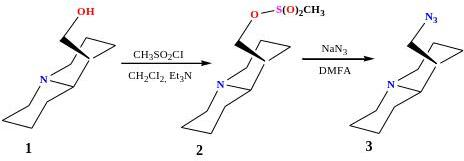
\includegraphics[width=0.8\textwidth]{assets/1011}
	\caption*{}
\end{figure}

Екінші сатыда лупинин азидінің \textbf{3} функционалды орынбасылған
ароматты ацетилендермен {[}фенилацетилен \textbf{4a},
4-этилфенилацетилен \textbf{4b}, 4-фторфенилацетилен \textbf{4c},
5-(этинил)этилантранилат \textbf{4d}, 3,4,5-триметоксифенилацетилен
\textbf{4e}, 4-бензилокси-3-метоксифенилацетилен \textbf{4f}{]} өзара
әрекеттесулері ДМФА ортасында мыс купоросы және натрийдің аскорбаты
қатысында 75°С температурада қыздыру арқылы жүзеге асырылды. Бұл реакция
Сu\textsuperscript{1} катализаторлық әсерімен 1,3-диполяры қосылу
механизмі бойынша жүреді:

\begin{figure}[H]
	\centering
	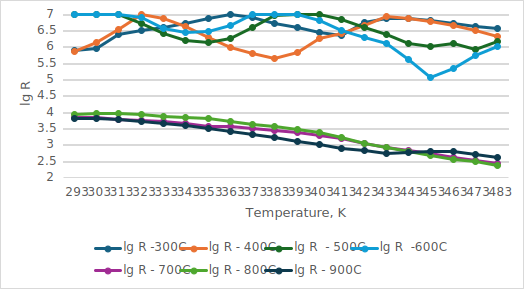
\includegraphics[width=0.8\textwidth]{assets/1012}
	\caption*{}
\end{figure}

\begin{figure}[H]
	\centering
	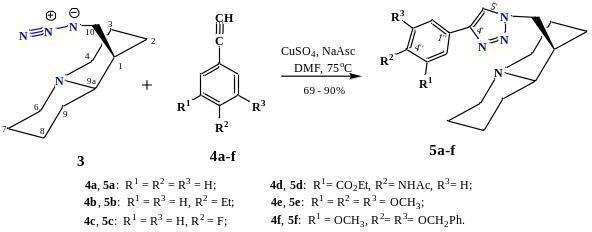
\includegraphics[width=0.8\textwidth]{assets/1013}
	\caption*{}
\end{figure}

Реакция жүру барысы ЖҚХ әдісімен бақыланды. Нәтижесінде бағаналы
хроматография әдісімен құрамында 1,2,3-үшазол циклінің С-4 жағдайындағы
арил-орынбасылған лупининнің үшазолды туындылары (\textbf{5а-f})
(шығымдары 69-90\%) таза түрде бөлініп алынды.

Синтезделген қосылыстардың құрамы мен құрылымы ИҚ-, ЯМР
\textsuperscript{1}Н- және \textsuperscript{13}С- спектроскопия және
масс-спектрометрия әдістерімен дәлелденілді. Лупинин азидінің \textbf{3}
құрылысында орынбасылған N\textsubscript{3-}тобының болуы ИҚ спектрінің
мәлімдемелерімен анықталды (2096 см\textsuperscript{-1} аймағында азид
тобының валенттік тербелістеріне сәйкес келетін қарқынды сіңіру жолағы
байқалды).

Синтезделген 1,2,3-үшазолды қосылыстардың ЯМР \textsuperscript{1}Н- және
\textsuperscript{13}C-спектрлерінде хинолизин қаңқасына тән және тиісті
орынбасылған фунционалды топтарға қатысты сигналдар жиынтығы кездеседі.
Күшті өріс аймағында (δ 1.17-1.70 м.ү.) интегралдық қарқындылығы 8Н
болатын кең мультиплеттік сигналдар орналасқан, олардың құрамына осьтік
және экваторлық бағыттағы лупинин қаңқасының протондары
(Н-2\emph{a},\emph{e},8\emph{a},\emph{e},9\emph{a},\emph{e},3\emph{a},7\emph{a})
кіреді. Мультиплет сигналы (δ 1.70-1.92 м.ү.) экваторлық бағытталған
H-3,7 протондарына қатысты. Әрі қарай 4,6 (δ 1.88-2.08 м.ү.) аксиальді
протондар, 9а (δ 2.05-2.18 м.ү) түйіндік протондар және С-1 (δ 2.18-2.30
м.ү) протондары резонанс тудырады. 4,6 Экваторлық бағыттағы протондар (δ
2.80-2.88 м.ү.) аймақтағы мультиплетпен ұсынылған. Н-10 метилен тобының
протондары δ 4.51-4.65 м.ү. аймағында екі дублет-дублет түрінде
резонанстық жағдайға әкеледі. \textbf{5a-f} Қосылыстардың ЯМР
\textsuperscript{1}H спектріндегі түзілген 1,2,3-үшазолдық циклдардың
протонына δ 7.37--7.71 м.ү. аймағында орналасқан синглетті сигнал жауап
береді. ЯМР \textsuperscript{13}C спектріндегі үшазол циклінің көміртегі
атомдары сәйкесінше 119.3--122.4 м.ү. (С-5) және 146.2--156.8 м.ү. (С-4)
дублет және синглет түрінде байқалады (спектрлер JMOD режимінде
жазылды). Бұл мәлімдемелер СuAС реакциялар нәтижесінде 1,4-орынбасылған
1\emph{H}-1,2,3-үшазолдардың түзілуін растайды {[}18,19{]}.

Барлық қосылыстардың масс-спектрлерінде әртүрлі қарқындылықтағы
молекулалық иондардың шыңдары кездеседі. Барлық синтезделген үшазолды
туындылардың \textbf{5а-f} спектрлерінде молекуланың хинолизидинді
қаңқасының С-10 атомы арқылы бөлінуіне сәйкес келетін
С\textsubscript{10}H\textsubscript{17}N (150-151 ш.б.) фрагментті
иондарының шыңдары сипатталған.

\textbf{Қорытынды.} Мақалада С-10 атомы бойынша лупинин алкалоидының
құрылымын түрлендірудің оңтайлы шарттары ұсынылды және жасалынды, оның
жоғары өнімділігі бар ықтимал биобелсенді 1,2,3-үшазол туындылары
синтезделді. Соңғы үшазол өнімдерін алу екі кезеңде жүзеге асырылды:
аралық лупинин азидінің синтезі және оның 1,3-екіполярлы
{[}3+2{]}-әртүрлі алкиндерге тұйықты қосылуы. Реакциялар ДМФА
еріткішінде мыс сульфаты және натрий аскорбатының қатысуымен жүргізілді.
Лупинин алкалоидының жаңа синтезделіп алынған 1,2,3-үшазолды фрагменті
бар туындылары биологиялық белсенді субстраттың қосымша
лиганд-рецепторлық өзара әрекеттесуін қамтамасыз ете алады және алынған
субстраттың биологиялық әсерінің селективтілігін өзгертеді. Синтезделген
жаңа қосылыстардың құрылыстары ЯМР \textsuperscript{1}H-,
\textsuperscript{13}С-спектроскопия және масс-спектрометрия әдістерімен
дәлелденілді.

\emph{\textbf{Қаржыландыру:} Жұмыс Қазақстан Республикасы Білім және
ғылым министрлігі Ғылым Комитетінің гранттық қаржыландыру жөніндегі
№АР23487712 жобасы шеңберінде орындалды}.

\textbf{Әдебиеттер}

1. Чудинов М.В., Константинова И.Д., Рыжова О.И., Есипов Р.С., Юркевич
А.М., Швец В.И., Мирошников А.И. Новый эффективный способ синтеза
5-замещенных производных 1,2,4-триазол-3-карбоксамида и рибавирина //
Химико-фармацевтический журнал, 2005. - № 4. - С. 43-46.

2. Клен Е.Е., Исхакова Г.Ф. Исследование реакций тиранов с
1,2,4-триазолами // Материалы республиканской конференции «Вопросы
теоретической и практической медицины». -- Уфа, 2000. - C. 51.

3. Pustolaikina I.A., Fazylov S.D., Nurmaganbetov Zh.S., Normatov S.Sh.,
Kim V.V. Computational study of lupinine and its derivatives for
dihydrofolat reductase inhibition // Program of the VII international
scientific-practical conference dedicated to the 50\textsuperscript{th}
anniversary of the Faculty of Chemistry and 100\textsuperscript{th}
anniversary of the First Dean professor R.G. Omarova. -Karaganda, 2023.
- P. 167.

4. Клен Е.E., Халюллин Ф.A., Спасов А.A., Макарова Н.Н., Багаутдинова
Л.Ф., Науменко Л.В. Синтез и геммореологические свойства новых
производств 1,2,4-триазола // Химико-фармацевтический журнал, 2008. - №
9. - С. 15-17.

5. Yengoyan A.P., Pivazyan V.A., Chazaryan E.A., Hakobyan R.S. Synthesis
of new thiazolo{[}3,2-b{]}{[}1,2,4{]}triazole derivatives and
preliminary evaluation of their biological activity // Journal of
General Chemistry,2019. -Vol.89(1) - P. 32-36. DOI
10.1134/S107036321901006

6. Popov S.A., Semenova M.D., Baev D.S., Frolova T.S., Shults E.E., Wang
Ch., Turkse M. Synthesis of cytotoxic urs-12-ene- and 28-nor-urs-12-ene-
type conjugates with amino- and mercapto-1,3,4-oxadiazoles and
mercapto-1,2,4-triazoles // Steroids,2020. - V.153:108524.

DOI 10.1016/j.steroids.2019.108524

7. Vagish C.B., Sudeep P., Jayadevappa H.P., Ajay Kumar K.
1,2,4-Triazoles: Synthetic and Medicinal Perspectives // International
Journal of Current Research, 2020. - Vol.12(8) - P. 12950-12960. DOI
10.24941/ijcr.39386.08.2020

8. Mobinikhaledi A., Foroughifar N., Khanpour M., Ebrahimi S. Synthesis
of Some Novel Schiff Bases Containing 1,2,4-Triazole Ring // Eur. J.
Chem., 2010. -Vol.1(1) - P. 33-36.

DOI 10.5155/eurjchem.1.1.33-36.5

9.Тилябаев З., Гафуров М.B., Далимов Д.Н., Абдувахабов А.A. Синтез
фосфорилированных продуктов алкалоидов, их структура, биологическая
активность и перспективы практического использования. - Ташкент: ФАН,
2017. - 185 c.

10. Ahmed B.A., Mohammed S.J. Improved Synthesis of
3-(α,α-Diphenyl-α-hydroxymethyl)-4-amino-1,2,4-triazoline-5-thione and
Facile Route to 3,6-Disubstituted
1,2,4-Triazolo{[}3,4-b{]}{[}1,3,4{]}-thiadiazoles // J. Raf. Sci., 2009.
-- Vol.20(4) - P. 11-16.

11. Feshin V.B., Feshin E.V. Ab initio Calculation of the Structure of
5-Chloro-1,2,4-triazole // Chem. Heter. Comp., 2001. -- Vol.37(1) - P.
95-99. DOI 10.1023/A:1017544902053

12. Абдувахабов А.A., Далимов Д.Н., Утениязов К.У., Асланов Х.A.
Лупинин. Нукус, 1993. - 198 c.

13.Sparatore A., Novelli F., Sparatore F. N-Homolupinanoyl and
N-(ω-lupinylthio)alkanoyl derivatives of some tricyclic systems as
ligands for muscarinic M1 and M2 receptor subtypes //
Farmaco,~2003.-Vol.58(9) - P. 669-676.
https://doi.org/10.1016/S0014-827X(03)00104-6

14.Salini M.J., Adams L.R. Growth performance, nutrient utilisation and
digestibility by Atlantic salmon (\emph{Salmo salar} L.) fed Tasmanian
grown white (\emph{Lupinus albus}) and narrow-leafed (\emph{Lupinus}
\emph{angustifolius}) lupins // Aquaculture, 2014.-Vol.426-427. - P.
296-303.

DOI 10.1016/j.aquaculture.2014.02.020

15.Tasso B., Catto M., Nicolotti O., Novelli F., Tonelli M., Giangreco
I., Pisani L., Sparatore A., Boido V., Carotti A., Sparatore F.
Quinolizidinyl derivatives of bi- and tricyclic systems as potent
inhibitors of acetyl- and butyrylcholinesterase with potential in
Alzheimer's disease // European Journal of Medicinal Chemistry. 2011.-
Vol.46(6)- P. 2170-2184.

https://doi.org/10.1016/j.ejmech.2011.02.071

16. Nurmaganbetov Zh.S., Fazylov S.D., Turdybekov K.M., Nurkenov O.A.,
Turdybekov D.M., Mukusheva G.K., Minayeva Ye.V., Khabdolda G. Synthesis
and Structure of 4-Substituted
(1S,9aR)-1-{[}(1,2,3-triazol-1-yl)methyl{]}octahydro-1H-quinolysines of
Lupinine // Bull. Univ. Karaganda Chem. 2022. -- Vol.106(2) - P. 12-22.
https://doi.org/10.31489/2022Ch2/2-22-5

17.Schepetkin I.A.~, Nurmaganbetov Zh.S., Fazylov S.D.~, Nurkenov O.A.,
Khlebnikov A.I.~, Seilkhanov T.M.~, Kishkentaeva A.S.~, Shults E.E.~,
Quinn M.T. Inhibition of Acetylcholinesterase by Novel Lupinine
Derivatives // Molecules\emph{,} 2023.-Vol.28(8) - P. 3357.

https://doi.org/10.3390/molecules28083357

18. Creary X., Anderson A., Brophy C., Crowell F., Funk Z. Method for
Assigning Structure of 1,2,3-Triazoles // J. Org. Chem., 2012. --
Vol.77(19) - P. 8756-8761. DOI 10.1021/jo301265t

19. Aday H.A. Synthesis and Characterization of the Triazole Derived
from Thiosemicarbazide, 4-Amino-5-phenyl-4H-1,2,4-triazole-3-thiol and
Their Copper(II) and Nickel(II) Complexes // Eng. \& Tech. J., 2013. --
Vol.31(2) - P. 216-221. DOI 10.30684/etj.31.2b.8

\begin{quote}
\textbf{References}
\end{quote}

1. Chudinov M.V., Konstantinova I.D., Ryzhova O.I., Esipov R.S.,
Jurkevich A.M., Shvec V.I., Miroshnikov A.I. Novyj jeffektivnyj sposob
sinteza 5-zameshhennyh proizvodnyh 1,2,4-triazol-3-karboksamida i
ribavirina // Himiko-farmacevticheskij zhurnal, 2005. - № 4. - S. 43-46.
{[}in Russian{]}

2. Klen E.E., Ishakova G.F. Issledovanie reakcij tiranov s
1,2,4-triazolami // Materialy respublikanskoj konferencii «Voprosy
teoreticheskoj i prakticheskoj mediciny». -- Ufa, 2000. - C. 51. {[}in
Russian{]}

3. Pustolaikina I.A., Fazylov S.D., Nurmaganbetov Zh.S., Normatov S.Sh.,
Kim V.V. Computational study of lupinine and its derivatives for
dihydrofolat reductase inhibition // Program of the VII international
scientific-practical conference dedicated to the 50\textsuperscript{th}
anniversary of the Faculty of Chemistry and 100\textsuperscript{th}
anniversary of the First Dean professor R.G. Omarova. -Karaganda, 2023.
- P. 167

4. Klen E.E., Haljullin F.A., Spasov A.A., Makarova N.N., Bagautdinova
L.F., Naumenko L.V. Sintez i gemmoreologicheskie svojstva novyh
proizvodstv 1,2,4-triazola // Himiko-farmacevticheskij zhurnal, 2008. -
№ 9. - S. 15-17.

5. Yengoyan A.P., Pivazyan V.A., Chazaryan E.A., Hakobyan R.S. Synthesis
of new thiazolo{[}3,2-b{]}{[}1,2,4{]}triazole derivatives and
preliminary evaluation of their biological activity // Journal of
General Chemistry,2019. -Vol.89(1) - P. 32-36. DOI
10.1134/S107036321901006

6. Popov S.A., Semenova M.D., Baev D.S., Frolova T.S., Shults E.E., Wang
Ch., Turkse M. Synthesis of cytotoxic urs-12-ene- and 28-nor-urs-12-ene-
type conjugates with amino- and mercapto-1,3,4-oxadiazoles and
mercapto-1,2,4-triazoles // Steroids,2020. - V.153:108524.

DOI 10.1016/j.steroids.2019.108524

7. Vagish C.B., Sudeep P., Jayadevappa H.P., Ajay Kumar K.
1,2,4-Triazoles: Synthetic and Medicinal Perspectives // International
Journal of Current Research, 2020. - Vol.12(8) - P. 12950-12960. DOI
10.24941/ijcr.39386.08.2020

8. Mobinikhaledi A., Foroughifar N., Khanpour M., Ebrahimi S. Synthesis
of Some Novel Schiff Bases Containing 1,2,4-Triazole Ring // Eur. J.
Chem., 2010. -Vol.1(1) - P. 33-36.

DOI 10.5155/eurjchem.1.1.33-36.5

9.Tiljabaev Z., Gafurov M.B., Dalimov D.N., Abduvahabov A.A. Sintez
fosforilirovannyh produktov alkaloidov, ih struktura, biologicheskaja
aktivnost\textquotesingle{} i perspektivy prakticheskogo
ispol\textquotesingle zovanija. - Tashkent: FAN, 2017. - 185 c.

10. Ahmed B.A., Mohammed S.J. Improved Synthesis of
3-(α,α-Diphenyl-α-hydroxymethyl)-4-amino-1,2,4-triazoline-5-thione and
Facile Route to 3,6-Disubstituted
1,2,4-Triazolo{[}3,4-b{]}{[}1,3,4{]}-thiadiazoles // J. Raf. Sci., 2009.
-- Vol.20(4) - P. 11-16.

11. Feshin V.B., Feshin E.V. Ab initio Calculation of the Structure of
5-Chloro-1,2,4-triazole // Chem. Heter. Comp., 2001. -- Vol.37(1) - P.
95-99. DOI 10.1023/A:1017544902053

12. Abduvahabov A.A., Dalimov D.N., Utenijazov K.U., Aslanov H.A.
Lupinin. Nukus, 1993. - 198 c.

14.Salini M.J., Adams L.R. Growth performance, nutrient utilisation and
digestibility by Atlantic salmon (\emph{Salmo salar} L.) fed Tasmanian
grown white (\emph{Lupinus albus}) and narrow-leafed (\emph{Lupinus}
\emph{angustifolius}) lupins // Aquaculture, 2014.-Vol.426-427. - P.
296-303.

DOI 10.1016/j.aquaculture.2014.02.020

15.Tasso B., Catto M., Nicolotti O., Novelli F., Tonelli M., Giangreco
I., Pisani L., Sparatore A., Boido V., Carotti A., Sparatore F.
Quinolizidinyl derivatives of bi- and tricyclic systems as potent
inhibitors of acetyl- and butyrylcholinesterase with potential in
Alzheimer's disease // European Journal of Medicinal Chemistry. 2011.-
Vol.46(6)- P. 2170-2184.

https://doi.org/10.1016/j.ejmech.2011.02.071

16. Nurmaganbetov Zh.S., Fazylov S.D., Turdybekov K.M., Nurkenov O.A.,
Turdybekov D.M., Mukusheva G.K., Minayeva Ye.V., Khabdolda G. Synthesis
and Structure of 4-Substituted
(1S,9aR)-1-{[}(1,2,3-triazol-1-yl)methyl{]}octahydro-1H-quinolysines of
Lupinine // Bull. Univ. Karaganda Chem. 2022. -- Vol.106(2) - P. 12-22.
https://doi.org/10.31489/2022Ch2/2-22-5

17.Schepetkin I.A.~, Nurmaganbetov Zh.S., Fazylov S.D.~, Nurkenov O.A.,
Khlebnikov A.I.~, Seilkhanov T.M.~, Kishkentaeva A.S.~, Shults E.E.~,
Quinn M.T. Inhibition of Acetylcholinesterase by Novel Lupinine
Derivatives // Molecules\emph{,} 2023.-Vol.28(8) - P. 3357.

https://doi.org/10.3390/molecules28083357

18. Creary X., Anderson A., Brophy C., Crowell F., Funk Z. Method for
Assigning Structure of 1,2,3-Triazoles // J. Org. Chem., 2012. --
Vol.77(19) - P. 8756-8761. DOI 10.1021/jo301265t

19. Aday H.A. Synthesis and Characterization of the Triazole Derived
from Thiosemicarbazide, 4-Amino-5-phenyl-4H-1,2,4-triazole-3-thiol and
Their Copper(II) and Nickel(II) Complexes // Eng. \& Tech. J., 2013. --
Vol.31(2) - P. 216-221. DOI 10.30684/etj.31.2b.8

\emph{\textbf{Авторлар туралы мәліметтер}}

Нұрмағанбетов Ж.С.- химия ғылымдарының кандидаты, қауымдастырылған
профессор, Қазақстан Республикасының органикалық синтез және көмір
химиясы институты, Қарағанды, е-mail: nzhangeldy@yandex.ru;

Нүркенов ОюАю- химия ғылымдарының докторы, профессор, Қазақстан
Республикасының органикалық синтез және көмір химиясы институты,
Қарағанды, е-mail: nurkenov\_oral@mail.ru;

Фазылов С.Д.- ҚР ҰҒА академиясының академигі, химия ғылымдарының
докторы, профессор, Қазақстан Республикасының органикалық синтез және
көмір химиясы институты, Қарағанды, е-mail: iosu8990@mail.ru;

Ибрайбекова А.М.-техника және технология магистрі, Қарағанды медицина
университеті, Қарағанды, е-mail: Ibraybekova@kgmu.kz;

Хабдолда Г. \textbf{-} химия ғылымдарының кандидаты, қауымдастырылған
профессор, Қарағанды медицина университеті, Қарағанды, е-mail:
Khabdoldag@mail.ru

Әшірбекова Б.- Медицина магистрі, Қарағанды медицина университеті,
Қарағанды, е-mail: ashirbekova@qmu.kz.

\emph{\textbf{Information about authors}}

Nurmaganbetov Zh.S.-Candidate of Chemical Sciences, Associate Professor
of the Institute of Organic Synthesis and Carbon Chemistry of the
Republic of Kazakhstan, Karaganda, е-mail: nzhangeldy@yandex.ru;

Nurkenov O.A.-Doctor of Chemical Sciences, Professor of the Institute of
Organic Synthesis and Coal Chemistry of the Republic of Kazakhstan,
Karaganda, е-mail: nurkenov\_oral@mail.ru;

Fazylov S.D.- аcademician NAS RK, Doctor of Chemical Sciences, Professor
of the Institute of Organic Synthesis and Carbon Chemistry of the
Republic of Kazakhstan, Karaganda, е-mail: iosu8990@mail.ru;

Ibraybekova A.M.- Master of Engineering and Technology of the Karaganda
Medical University, Karaganda, е-mail: Ibraybekova@kgmu.kz;

Khabdolda G. \textbf{-} Candidate of Chemical Sciences, Associate
Professor of the Karaganda Medical University, Karaganda, e-mail:
Khabdoldag@mail.ru;

Ashirbekova B. -- Master of Medicine of the Karaganda Medical
University, Karaganda, e-mail: ashirbekova@qmu.kz

МРНТИ 31.15.37

\textbf{Способ получения СУПЕРГИДРОФОБНОЙ ГЛИНЫ месторождения}

\textbf{«Таганское» для производства БУРОВЫХ РАСТВОРОВ}

\textbf{\textsuperscript{1,3} O.В. Рожкова, \textsuperscript{1,2}Д.M-K.
Ибраимов, \textsuperscript{3,4}В.И Рожков, \textsuperscript{1}М.Т.
Ермеков,}

\textbf{\textsuperscript{3}С.Ж.Кудайбергенова,
\textsuperscript{3}А.Б.Букеева, \textsuperscript{5}Ж.Т.Нуртай}

\textsuperscript{1} АО «Science and Technology Solutions», г. Алматы,
Казахстан,

\textsuperscript{2} НАО «Казахский национальный университет имени
Аль-Фараби»,

г. Алматы, Казахстан,

\textsuperscript{3} НАО \textsuperscript{«}Казахский~агротехнический
исследовательский университет им.~С.~Сейфуллина»,

г. Астана, Казахстан,

\textsuperscript{4} ТОО «Алтайский геолого-экологический институт», г.
Усть-Каменогорск, Казахстан,

\textsuperscript{5} АО «Казахский Университет технологии и бизнеса им
К.Кулажанова», г. Астана, Казахстан,

Корреспондент-автор: rozhkova.o@stsolutions.kz

В данной работе нами был изучен способ получения из бентонитовой глины
месторождения «Таганское» органофильной глины с краевым углом более
150°, обладающую высокой устойчивостью в органической среде, с целью
дальнейшего создания буровых растворов на ее основе, проявляющих
тиксотропные свойства в безводной среде.

В ходе проведения исследований нами был разработан новый способ
получения супергидрофобных глин из бентонитовой глины, а также изучено
их дальнейшее применение в производстве безводных буровых растворов для
нефтедобывабщей промышленности. В качестве супергидрофобизаторов нами
были использованы самые разнообразные катионные поверхностно-активные
вещества.

В присутствии тетракис(децил) бромид аммония (ТКБА) была получена
органофильная (супергидрофобная) глина с углом смачивания 170º. Было
определено распределение и устойчивость частиц органофильных глин в
дизельном топливе, полученным методом ТКБА. Доказано, что частицы
органофильной глины, полученные на основе ТКБА, образуют стабильную
суспензию в дизельном топливе и совершенно не смешиваются с водной
фазой.,

\textbf{Ключевые слова:} супергидрофобная глина, буровой раствор,
технология, поверхностно-активные вещества, месторождение «Таганское»,
бентонит.

\textbf{Бұрғылау ерітінділерін өндіру мақсатында "ТАҒАН" кен орнының
супергидрофобты сазын алу тәсілі}

\textbf{\textsuperscript{1,3} O.В. Рожкова, \textsuperscript{1,2}Д.M-K.
Ибраимова, \textsuperscript{3,4}В.И Рожков, \textsuperscript{1}М.Т.
Ермеков,}

\textbf{\textsuperscript{3}С.Ж.Кудайбергенова,
\textsuperscript{3}А.Б.Букеева, \textsuperscript{5}Ж.Т.Нұртай}

\textsuperscript{1} «Science and Technology Solutions», АҚ, Алматы,
Қазақстан,

\textsuperscript{2} КЕАҚ «Әл-Фараби атындағы Қазақ ұлттық университеті»,
Алматы, Қазақстан,

\textsuperscript{3} КЕАҚ «С.Сейфуллин атындағы Қазақ агротехникалық
зерттеу университеті", Астана қ., Қазақстан,

\textsuperscript{4} Алтай геологиялық-экологиялық институты" ЖШС,
Өскемен қ., Қазақстан,

\textsuperscript{5} «Қ.Құлажанов атындағы Қазақ технология және бизнес
университеті» АҚ, Астана, Қазақстан

e-mail: rozhkova.o@stsolutions.kz

Бұл жұмыстың мақсаты - "Таған" кенорнының бентонит сазынан органикалық
ортада жоғары тұрақтылыққа ие 150° - тан асатын органофильді саз алу
әдісін, сондай-ақ, одан сусыз ортада тиксотропты қасиет көрсететін
бұрғылау ерітінділерін жасау әдісін зерттеу.

Зерттеу барысында бентонит сазынан супергидрофобты саздарды алудың жаңа
әдісін әзірленді, сонымен қатар, олардың мұнай өндіру өнеркәсібі үшін
сусыз бұрғылау ерітінділерін өндіруде одан әрі қолданылуы зерттелді.
Супергидрофобизаторлар ретінде катионды беттік активті заттардың алуан
түрін қолданылған.

Тетракис (децил) аммоний бромиді қатысында жұғу бұрышы(ТКАБ) 170º
органофильді (супергидрофобты) саз алынды. ТКАБ негізінде алынған дизель
отынындағы органофильді саз бөлшектерінің таралуы мен тұрақтылығы
анықталды. ТКБА-дан алынған органофильді саз бөлшектері дизельде тұрақты
суспензия түзетіні және су фазасымен мүлдем араласпайтыны дәлелденді.

\textbf{Түйін сөздер:} супергидрофобты саз, бұрғылау сұйықтығы,
технология, беттік белсенді заттар, Таганское кен орны, бентонит.

\textbf{PRODUCING METHOD FOR SUPERHYDROPHOBIC CLAY TAGANSKOYE DEPOSIT
FOR THE DRILLING FLUIDS PRODUCTION}

\textbf{\textsuperscript{1,3}O.V Rozhkova,
\textsuperscript{1,2}D.M-K.Ibraimova, \textsuperscript{3,4} V.I.Rozhkov,
\textsuperscript{1} M.T.Yermekov,}

\textbf{\textsuperscript{3}S.J. Kudaibergenova,
\textsuperscript{3}A.B.Bukeeva, \textsuperscript{5}Zh.T.Nurtai}

\textsuperscript{1} SC "Science and Technology Solutions", Almaty,
Kazakhstan,

\textsuperscript{2} NC JSC "Al-Farabi Kazakh National University",

Almaty, Kazakhstan,

\textsuperscript{3} NAO "S. Seifullin Kazakh Agrotechnical Research
University", Astana, Kazakhstan,

\textsuperscript{4}Altai Geological and Ecological Institute LLP,
Ust-Kamenogorsk, Kazakhstan,

\textsuperscript{5} JSC ``Kazakh University of Technology and Business
named after K. Kulazhanov'', Astana, Kazakhstan,

e-mail: rozhkova.o@stsolutions.kz

In this work, we studied a method for producing organophilic clay with a
contact angle of more than 150° from bentonite clay from the Taganskoye
deposit, demonstrating high stability in an organic environment, with
the aim of further creating drilling fluids based on it, exhibiting
thixotropic properties in an anhydrous environment.

During the course of our research, A novel method for producing
superhydrophobic clays from bentonite have been developed and explored
their potential applications in the production of anhydrous drilling
fluids for the petroleum industry.

A variety of cationic surfactant compounds were used as superhydrophobic
agents.In the presence of tetrakis(decyl) ammonium bromide (TKAB),
organophilic (superhydrophobic) clay with a wetting angle of 170 degrees
was obtained. The distribution and stability of organophilic clay
particles obtained using TKAB in diesel fuel were determined. It was
proved that the particles of organophilic clay formed on the basis of
TKAB create a stable suspension in diesel fuel and do not mix with the
aqueous phase at all.

\textbf{Keywords:} superhydrophobic clay, drilling fluid, technology,
surfactants, Taganskoye deposit, bentonite.

\textbf{Введение.} В настоящее время, значительно возрос интерес к
бентонитовым глинам месторождения, которых встречаются на всех
континентах нашей планеты. Известно, что в природе бентониты различаются
не только по химико-минералогическому составу и физико-химическим
свойствам, но и внешним признакам. Так, интерес вызывают исследования
связанные с получением композитных глинистых материалов, в частности для
производства органомодифицированных глин (органоглин). В этой связи,
производители зачастую сталкиваются с проблемой поиска качественного
сырья для организации производства.

Ведущими мировыми производителями органоглин являются в основном
зарубежные компании, такие как Rockwood, Southern Clay Рroducts Inc.
(Cloisit, США), Sued Chemie AG (Nanofil, Германия). Для примера,
органоглина является основным наполнителем буровых растворов при бурении
нефтяных скважин, а Казахстан очень богат разнообразием глин пригодных
для их производства. Однако вследствие малоизученности этих глин, они в
настоящее время не востребованы. Несмотря на наличие достаточно обширной
информации о свойствах различных глин на территории Казахстана, имеется
лишь незначительное количество систематизированных научных работ по
возможному получению органоглин из отечественного сырья {[}1-8{]}.

В этой связи, перед нами возник интерес в проведении исследований
бентонитовой глины месторождения «Таганское» для получения органоглин
применительно к буровым растворам, поскольку они отличаются высоким
содержанием монтмориллонита, порядка 95\%. На месторождении «Таганское»
(Тарбагатайский район, Восточно-Казахстанская область, Республика
Казахстан) из-за особенностей генезиса выявлены 3 вида бентонитовой
глины: щелочной, щелочноземельный и фармацевтический, которые обладают
различными свойствами и содержанием монтмориллонита, что позволяет
использовать их в различных промышленных технологиях, в том числе и при
получении буровых растворов.

Бентонитовая глина 12-го горизонта месторождения «Таганское» на
сегодняшний день наиболее известна, так как по качественным
характеристикам она превосходит эталонный Вайомингский бентонит (США).
Ее адсорбционные свойства настолько хороши, что глина экспортируется во
Францию в качестве энтеросорбента.

Уникальность наших проводимых исследований состоит в том, что до
настоящего времени не применялись методы супергидрофобизации
монтмориллонита Таганского месторождения. Результаты ранее проведенных
нами исследований к настоящему времени приведены в статье {[}9{]} где в
качестве супергидрофобизатора использовался октадециламин и с краевым
углом смачивания 157° {[}9{]}.

Также, в некоторых работах {[}1-11{]} были проведены исследования по
получению органоглины из глин с использованием различных модификаторов,
при этом краевой угол смачивания в этих работах достигал 150°.

В данной работе, перед нами стояла задача - получить органоглину,
которая будет вводится в жидкость с очень низкой полярностью, и для
получения тиксотропных буровых растворов со стабильными свойствами
предлагается создать оптимальную органоглину. Для этого уникальная
бентонитовая глина месторождения «Таганское», из-за высокого содержания
монтмориллонита, имеет больше возможности для супергидрофобизации,
супрамолекулярной интеркаляции молекулами модификаторов.

Таким образом, целью данной работы является изучение способа получения
из монтмориллонита месторождения «Таганское» органофильной глины с
краевым углом более 150°, обладающую высокой устойчивостью в
органической среде, и предложить способ создания на его основе буровых
растворов, проявляющих тиксотропные свойства в безводной среде.

Новизна данной работы заключается в том, что нами впервые были получены
супергидрофобные органоглины на основе бентонита месторождения
«Таганское», краевой угол смачивания которых составил 170°, определена
пригодность полученной органоглины для приготовления бурового раствора и
предложены технологические схемы получения органоглины и создания
бурового раствора на их основе.

\textbf{Материалы и методы.} В данной работе использовался
Na-монтмориллонит, полученный из бентонитовых глин месторождения
«Таганское» (карьер 12). Основой является условная химическая формула
бентонита
(OH)\textsubscript{4}Si\textsubscript{8}Al\textsubscript{4}O\textsubscript{20}·n(межпакетная)H\textsubscript{2}O.
Таганский бентонит имеет светло-розовый цвет с темно-розовыми пятнами.
Вследствие того, что в большинстве случаев существуют разные его виды,
данный тип иногда называют Таганским фармацевтическим бентонитом.

Монтмориллониты как рядовой материал не проявляют выраженной
каталитической и адсорбционной активности, поэтому их необходимо
предварительно активировать или преобразовать. Для очистки глины от
примесей ее промывали методом декантации, а затем использовали метод
термокислотной активации. Монтмориллонит сначала высушивали при
температуре 90°C в течение 2 часов, глину смешивали в соотношении 1:3 с
15\% серной кислотой, затем непрерывно перемешивали при температуре 90°C
в течение 2 часов, нагревали в растворе кислоты на водяной бане. Через 2
часа бентонит отфильтровали, поместили на фарфоровую пластину и промыли
водным раствором аммиака, затем дистиллированной водой, пока значение pH
не достигло нейтрального значения. Затем фильтрат бентонита высушивали в
лабораторной сушилке при температуре 80°C в течение. Из него получают
высушенный активированный монтмориллонит, просеивают через сито и
помещают в стеклянную коническую колбу с пришлифованной пробкой.

\begin{figure}[H]
	\centering
	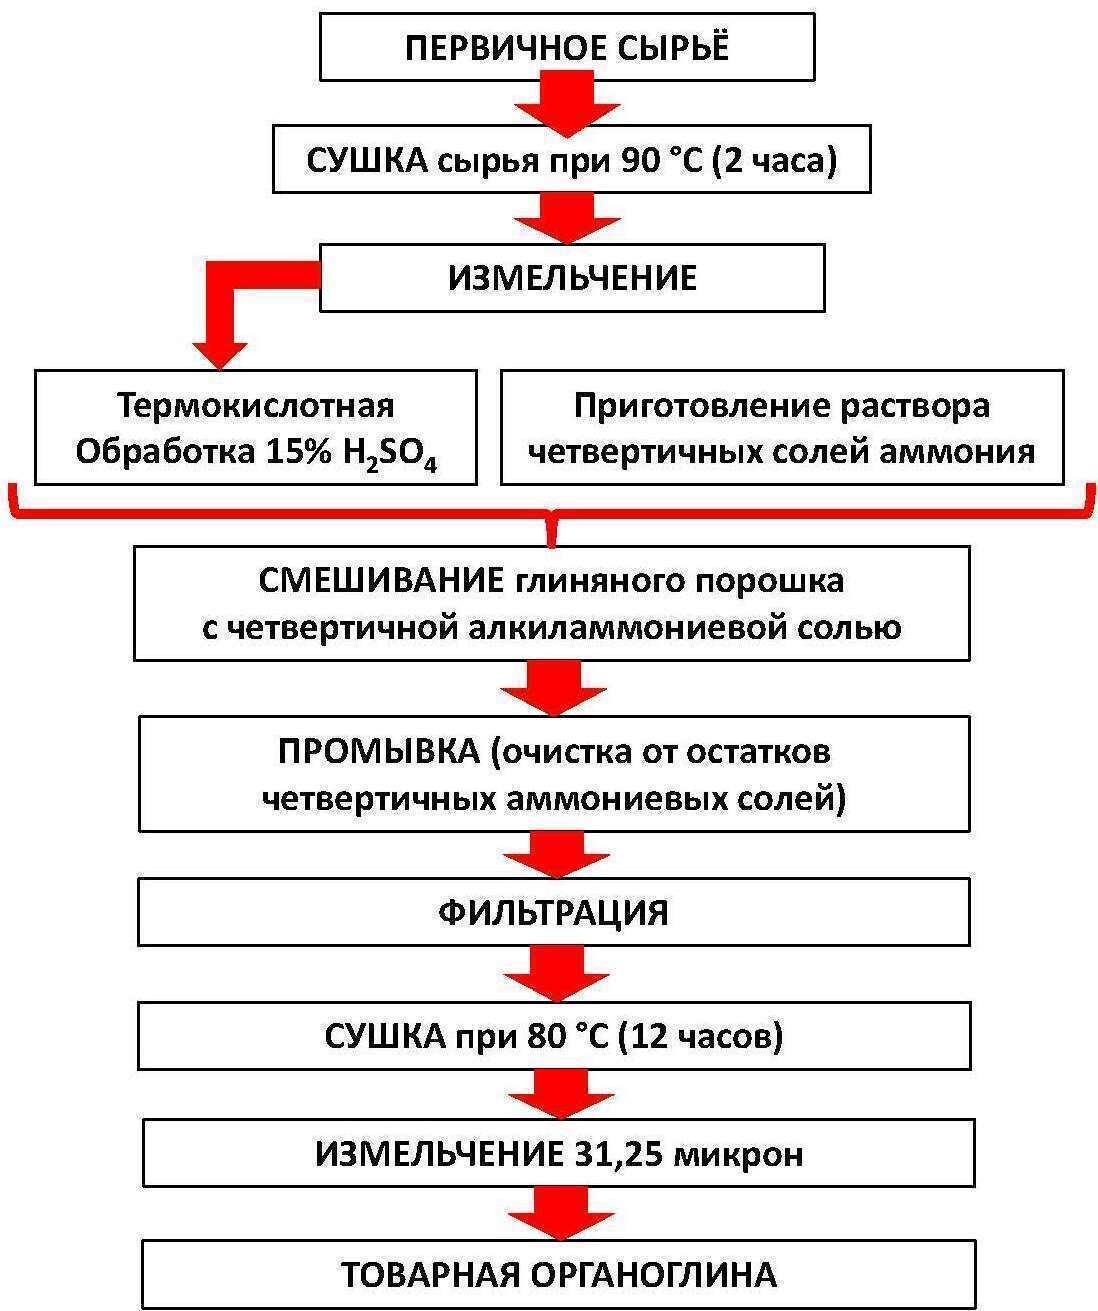
\includegraphics[width=0.8\textwidth]{assets/1014}
	\caption*{}
\end{figure}

\textbf{Рис. 1 -Технологическая схема производства органоглины}

Рентгенодифрактометрический (XRD) метод исследования был проведен на
автоматическом дифрактометре ДРОН 3.0 с
\emph{Cu}К\emph{\textsubscript{α}}-излучением и β-фильтром. Условия
съемки дифрактограмм: U=35кВ; I=20мА; θ-2θ захват; детектор 2 град/мин.
Рентгенофазовый анализ на полуколичественной основе проводился по
дифрактограммам образцов порошка методом равных суспензий и
искусственных смесей. Было определено количественное соотношение
кристаллических фаз. Интерпретация дифрактограмм проводилась с
использованием данных из картотеки Международного центра дифракционных
данных (icdd): PDF2 порошковая дифрактометрическая база данных
(порошковая дифрактометрия) и дифрактограммы чистых от примесей
минералов. Расчет содержания проводился для основных этапов.

В качестве гидрофобизаторов для обработки Na-монтмориллонита в работе
использовались несколько поверхностно-активных веществ (ПАВ) {[}12{]}:

\begin{enumerate}
\def\labelenumi{\arabic{enumi})}
\item
  Тетракис (децил)бромид аммония (ТКБА) -
  C\textsubscript{40}H\textsubscript{84}BrN
\item
  Дидецилдиметиламмоний бромид (ДЦДMAБ) -
  C\textsubscript{22}H\textsubscript{48}BrN
\item
  Триметилоктадециламмоний бромид (ТМOДАБ)
  C\textsubscript{21}H\textsubscript{46}BrN
\item
  Бромид цетилпиридиния (БЦП) C\textsubscript{21}H\textsubscript{38}BrN
\item
  Октадециламин (ОДА) C\textsubscript{18}H\textsubscript{39}N
\end{enumerate}

\begin{quote}
Реагенты, необходимые для создания буровых растворов:
\end{quote}

В качестве органомодифицированной глины (органоглины) использовалась
супергидрофобная глина, полученная путем модификации Таганского
Na-монтмориллонита ТКБА. Обычно органоглины применяются как
структурообразующий компонент, как регулятор реологических свойств
бурового раствора, также органоглина играет роль коркообразуемого
компонента, служащего для снижения водопоглощаемости ствола скважины.

\begin{quote}
1) Приготовление растворов гидрофобизаторов и обработка глины
проводилась по следующей методике:
\end{quote}

В процессе гидрофобизации готовили 100 мл растворов ПАВ в концентрации 1
М и 0,1 М. В приготовленные растворы помещали Na-монтмориллонитовую
глину в диапазоне 1-5 грамм и перемешивали в течение 5-6 часов в
подогреваемом лабораторном магнитной мешалке при температуре
70\textsuperscript{0} C. Порошок помещали в чашку Петри и сушили в
лабораторной сушилке до стабилизации веса, затем измельчали и просеивали
до размера 0,315 микрон. После этого определялась гидрофобность типов
органоглин.

2) Для характеристики морфологических особенностей глины использовался
метод просвечивающей электронной микроскопии {[}13{]}.

3) Гониометр ЛК-1 использовался для измерения контактного угла капли,
лежащей на поверхности порошка гидрофобной глины, по методике
стационарной лежащей неподвижной капли. Гониометр ЛК-1 создан на базе
горизонтального микроскопа и цифровой HD-видеокамеры и имеет возможности
для расчета угла контакта неподвижной капли с дисплеем {[}14{]}. Перед
определением контактных углов капель воды на поверхности гидрофобного
порошка органоглины, порошок продавливали через две стеклянные пластинки
и разглаживали.

4) Определение устойчивости супергидрофобных видов глины в средах
органических соединений. Дизельное топливо (дизтопливо) использовалось в
качестве жидкости с низкой диэлектрической проницаемостью для проверки
способности супергидрофобных глин диспергироваться в органических
средах. Приблизительная химическая формула дизтоплива: имеются
органические соединения из C\textsubscript{8}H\textsubscript{18} to
C\textsubscript{17}H\textsubscript{36}. Дизельное топливо представляет
собой сложную смесь парафиновых - предельных 10-40\% (общая формула
CnH2n+2), нафтеновых - полиметиленовых 20-60\% (общая формула CnH2n) и
ареновых - ароматических 14-30\% (общая формула CnH2n-6) углеводородов и
их производных средней молекулярной массы 110-230 г/моль, выкипающих в
пересчете на 170-380 ºC. Диэлектрическая постоянная дизтоплива
приблизительно ε=2,05 {[}15{]}.

5) Определение стабильности дисперсной среды путем осаждения в
органической среде проводилось с помощью фотоэлектрокалориметра.

6) Методы дифференциальной сканирующей калориметрии и термогравиметрии
(ДСК и ТГ) использовались для контроля влияния химических изменений в
составе органоглины под воздействием температуры, поскольку буровые
растворы могут подвергаться воздействию чрезвычайно высоких температур в
недрах земли. Эти методы проводились для изучения физико-химических и
химических процессов, происходящих в веществе при контролируемом
изменении температуры.

7) Реологические свойства буровых растворов и нефти на месторождении
Кумколь, взятых в качестве образцов, определялись простыми косвенными
методами. Например, были проведены такие измерения, как определение
плотности жидкости с помощью ареометра, определение pH раствора с
помощью pH-метра и определение вязкости с помощью реометра. Взаимосвязь
между скоростью сдвига и напряжением сдвига нефти на месторождении
Кумколь и буровых растворов на основе органоглины ТКБА определяли на
реометре MCR 702 MultiDrive (Anton Paar).

\textbf{Результаты и обсуждение.} Глинистые минералы содержат различные
типы алюмосиликатов, основные типы которых сменяют друг друга в
природных условиях в течение миллиардов лет {[}16-18{]}. Алюмосиликатный
скелет в глинах состоит в основном из чередующихся параллельных
двумерных слоев, образованных силикатными тетраэдрами и алюминиевыми
октаэдрами {[}19-21{]}. Расположение таких слоев, степень и характер
обмена в них определяют химические и физические свойства материалов,
включая адсорбционные свойства.

Природные алюмосиликаты можно разделить на две группы в зависимости от
их кристаллической решетки - кристаллические и аморфные {[}21-22{]}.
Аморфные алюмосиликаты характеризуются способностью набухать в процессе
ионного обмена, аналогично ионообменным смолам.

На всем месторождении «Таганское» выделяют 3 вида бентонитовой глины -
щелочную (розового цвета), щелочноземельную и фармацевтическую.
Благодаря особенностям генезиса месторождения «Таганское», различные
свойства монтмориллонитов и бентонитовых глин позволяют использовать их
в различных промышленных технологических линиях. Щелочные бентониты
используются для производства буровых растворов.

С целью определения полного химического состава глины был проведен
рентгенофлуоресцентный анализ (таблица 1).

\textbf{Таблица 1-Оксидный химический состав бентонитовой глины
месторождения «Таганское»}

\begin{longtable}[]{@{}
  >{\raggedright\arraybackslash}p{(\columnwidth - 16\tabcolsep) * \real{0.3509}}
  >{\raggedright\arraybackslash}p{(\columnwidth - 16\tabcolsep) * \real{0.0664}}
  >{\raggedright\arraybackslash}p{(\columnwidth - 16\tabcolsep) * \real{0.0713}}
  >{\raggedright\arraybackslash}p{(\columnwidth - 16\tabcolsep) * \real{0.0769}}
  >{\raggedright\arraybackslash}p{(\columnwidth - 16\tabcolsep) * \real{0.0762}}
  >{\raggedright\arraybackslash}p{(\columnwidth - 16\tabcolsep) * \real{0.0747}}
  >{\raggedright\arraybackslash}p{(\columnwidth - 16\tabcolsep) * \real{0.0734}}
  >{\raggedright\arraybackslash}p{(\columnwidth - 16\tabcolsep) * \real{0.0670}}
  >{\raggedright\arraybackslash}p{(\columnwidth - 16\tabcolsep) * \real{0.1433}}@{}}
\toprule\noalign{}
\begin{minipage}[b]{\linewidth}\raggedright
\textbf{Содержание}

\textbf{оксидов в минерале}
\end{minipage} & \begin{minipage}[b]{\linewidth}\raggedright
\textbf{СаO}
\end{minipage} & \begin{minipage}[b]{\linewidth}\raggedright
\textbf{MgO}
\end{minipage} & \begin{minipage}[b]{\linewidth}\raggedright
\textbf{Fe\textsubscript{2}O\textsubscript{3}}
\end{minipage} & \begin{minipage}[b]{\linewidth}\raggedright
\textbf{Al\textsubscript{2}O\textsubscript{3}}
\end{minipage} & \begin{minipage}[b]{\linewidth}\raggedright
\textbf{SiO\textsubscript{2}}
\end{minipage} & \begin{minipage}[b]{\linewidth}\raggedright
\textbf{Na\textsubscript{2}O}
\end{minipage} & \begin{minipage}[b]{\linewidth}\raggedright
\textbf{K\textsubscript{2}O}
\end{minipage} & \begin{minipage}[b]{\linewidth}\raggedright
\textbf{Остатки после сжигания}
\end{minipage} \\
\midrule\noalign{}
\endhead
\bottomrule\noalign{}
\endlastfoot
Количественное соотношение оксидов в сыром минерале монтмориллоните, \%
& 15 & 4 & 6 & 10 & 30 & 1,5 & 4 & 69,5 \\
Количественное соотношение оксидов в минерале Na-монтмориллонит, \% & 4
& 0,9 & 4 & 9,8 & 31 & 0,6 & 0,91 & 84,8 \\
\end{longtable}

Было обнаружено, что в составе бентонитовой глины наряду с элементами
Fe, Al, Si, Zn, Ti, Ca, Mn присутствует множество других элементов и
оксидов. При определении элементного состава, показано, что состав
монтмориллонита местрождения «Таганское» является кальциево-натриевым,
причиной чего является большое количество кальция.

При выполнении стадии декантационной промывки, термоактивации и
кислотной активации монтмориллонита месторождения «Таганское» удаляются
ионы кальция и магния. В результате чего увеличивается набухаемость,
ионообменная способность и межпакетное пространство глины.

С точки зрения природы монтмориллонита известно, что он
самодиспергируется в водной среде и распадается на отдельные пластинки
толщиной до 1 нм, диаметром 200-250 нм {[}23-24{]}.

\begin{figure}[H]
	\centering
	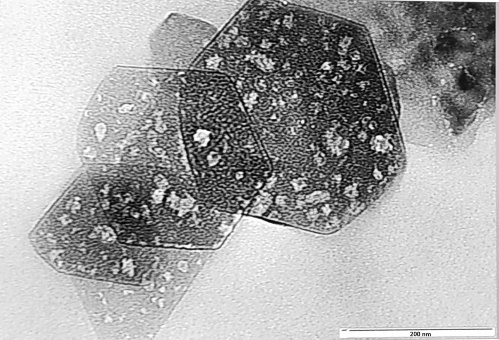
\includegraphics[width=0.8\textwidth]{assets/1015}
	\caption*{}
\end{figure}

\textbf{Рис. 2. - Результаты анализа методом просвечивающей электронной
микроскопии монтмориллонита месторождения «Таганское»}

С целью определения минерального состава бентонита месторождения
«Таганское»

и органоглины был проведен рентгенофазовый анализ. Полученные результаты
представлены в таблице 2.

\textbf{Таблица 2- Минеральный состав таганского бентонита}

\begin{longtable}[]{@{}
  >{\raggedright\arraybackslash}p{(\columnwidth - 4\tabcolsep) * \real{0.2170}}
  >{\raggedright\arraybackslash}p{(\columnwidth - 4\tabcolsep) * \real{0.5108}}
  >{\raggedright\arraybackslash}p{(\columnwidth - 4\tabcolsep) * \real{0.2722}}@{}}
\toprule\noalign{}
\begin{minipage}[b]{\linewidth}\raggedright
\textbf{Минерал}
\end{minipage} & \begin{minipage}[b]{\linewidth}\raggedright
\textbf{Формула}
\end{minipage} & \begin{minipage}[b]{\linewidth}\raggedright
\textbf{Количество, \%}
\end{minipage} \\
\midrule\noalign{}
\endhead
\bottomrule\noalign{}
\endlastfoot
Монтмориллонит & (Na,Н)\textsubscript{0.3}(Al,Mg,
Ca)\textsubscript{2}Si\textsubscript{4}O\textsubscript{10}(OH)\textsubscript{2}·xH\textsubscript{2}O
& 96,4 \\
Кварц & SiO\textsubscript{2} & 3,6 \\
\end{longtable}

\textbf{Таблица 3 - Минеральный состав органоглины, полученной с помощью
ТКБА}

\begin{longtable}[]{@{}
  >{\raggedright\arraybackslash}p{(\columnwidth - 4\tabcolsep) * \real{0.2170}}
  >{\raggedright\arraybackslash}p{(\columnwidth - 4\tabcolsep) * \real{0.5108}}
  >{\raggedright\arraybackslash}p{(\columnwidth - 4\tabcolsep) * \real{0.2722}}@{}}
\toprule\noalign{}
\begin{minipage}[b]{\linewidth}\raggedright
\textbf{Минерал}
\end{minipage} & \begin{minipage}[b]{\linewidth}\raggedright
\textbf{Формула}
\end{minipage} & \begin{minipage}[b]{\linewidth}\raggedright
\textbf{Количество, \%}
\end{minipage} \\
\midrule\noalign{}
\endhead
\bottomrule\noalign{}
\endlastfoot
Монтмориллонит & (Na,Н)\textsubscript{0.3}(Al,Mg,
Ca)\textsubscript{2}Si\textsubscript{4}O\textsubscript{10}(OH)\textsubscript{2}·xH\textsubscript{2}O
& 94-97 \\
Кварц & SiO\textsubscript{2} & 2-4 \\
Аморфная фаза & - & 1-2 \\
\end{longtable}

В результате определения минерального состава бентонита месторождения
«Таганское» и органоглины методом рентгеноструктурного анализа было
установлено, что в составе глины, наряду с минералом монтмориллонитом,
встречаются и другие минералы в виде кварца и аморфных фаз.

В настоящее время используется несколько методов гидрофобизации
монтмориллонита. Наиболее распространенные методы гидрофобизации
монтмориллонита включают в себя методы модификации поверхности, метод
интеркаляции модификаторов и метод биогидрофобизации {[}25{]}.

Каждый из этих методов имеет как свои преимущества, так и недостатки.
Выбор того или иного метода, напраямую зависит от цели проводимого
исследования, а также от предьявляемых требований к конечному продукту
{[}26{]}. Но более подходящим и выгодным для этого направления работ
является органомодификации - метод интеркаляции, потому как, есть
необходимость учитывать кристаллическую структуру монтмориллонита.

В структурных схемах некоторые ионы
\emph{Si\textsuperscript{4}}\textsuperscript{+} обмениваются на ионы
\emph{Al\textsuperscript{3+}}. В связи с перемещением мест
\emph{Al\textsuperscript{3+}} вместо
\emph{Si\textsuperscript{4}}\textsuperscript{+} в их кристалле создается
избыточный отрицательный заряд, который компенсируется катионами
щелочных и щелочноземельных металлов, которые не связаны с определенными
местами в решетке, подвижны и могут обмениваться на другие катионы
{[}23,27-35{]}. Соответственно, глинистые частицы могут иметь
некомпенсированный отрицательный заряд на поверхности, и также при
всплытии глинистых частиц взаимодействие между аминогруппами и
глинистыми частицами может осуществляться также за счет образования
водородных связей.

Механизм адсорбции катионных ПАВ на поверхности глинистых частиц
осуществляется за счет электростатического взаимодействия. Поскольку
используемый глинистый минерал является слоистым минералом, то метод
интеркаляции эффективен как метод гидрофобизации, и основной задачей
является выбор оптимального гидрофобизатора. Далее на поверхность
различных гидрофобизаторов и обработанного порошка монтмориллонита
наносили каплю воды и измеряли значения углов смачивания этих образцов с
помощью Гониометра ЛК-1. В таблице 4 приведены значения контактных
углов, полученные для каждой из органоглин.

\textbf{Таблица 4- Контактные углы капель воды, применяемых на
поверхности различных типов органомодифицированных глинопорошков}

% \begin{longtable}[]{@{}
%   >{\raggedright\arraybackslash}p{(\columnwidth - 8\tabcolsep) * \real{0.3900}}
%   >{\raggedright\arraybackslash}p{(\columnwidth - 8\tabcolsep) * \real{0.1166}}
%   >{\raggedright\arraybackslash}p{(\columnwidth - 8\tabcolsep) * \real{0.0874}}
%   >{\raggedright\arraybackslash}p{(\columnwidth - 8\tabcolsep) * \real{0.1894}}
%   >{\raggedright\arraybackslash}p{(\columnwidth - 8\tabcolsep) * \real{0.2167}}@{}}
% \toprule\noalign{}
% \multirow{2}{*}{\begin{minipage}[b]{\linewidth}\raggedright
% Пространственная
% 
% формула модификаторов
% \end{minipage}} &
% \multicolumn{2}{>{\raggedright\arraybackslash}p{(\columnwidth - 8\tabcolsep) * \real{0.2039} + 2\tabcolsep}}{%
% \begin{minipage}[b]{\linewidth}\raggedright
% Концентрации модификаторов и растворов монтмориллонита
% \end{minipage}} & \begin{minipage}[b]{\linewidth}\raggedright
% Контактный угол для монтмориллонита с органофильным покрытием
% \end{minipage} & \begin{minipage}[b]{\linewidth}\raggedright
% Изображения органоглины, в присутствии различных гидрофобизаторов
% \end{minipage} \\
% &
% \multicolumn{2}{>{\raggedright\arraybackslash}p{(\columnwidth - 8\tabcolsep) * \real{0.2039} + 2\tabcolsep}}{%
% \begin{minipage}[b]{\linewidth}\raggedright
% Монтмориллонит
% \end{minipage}} & \begin{minipage}[b]{\linewidth}\raggedright
% 31\textsuperscript{⁰}
% \end{minipage} & \begin{minipage}[b]{\linewidth}\raggedright
% \begin{figure}[H]
% 	\centering
% 	
\includegraphics[width=0.8\textwidth]{assets/1016}
% 	\caption*{}
% \end{figure}
% \end{minipage} \\
% \midrule\noalign{}
% \endhead
% \bottomrule\noalign{}
% \endlastfoot
% \multirow{2}{*}{\begin{figure}[H]
% 	\centering
% 	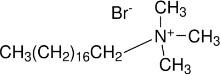
\includegraphics[width=0.8\textwidth]{assets/1017}
% 	\caption*{}
% \end{figure}}
% & \multirow{2}{*}{ТМOДАБ} & 0.1 М & 39\textsuperscript{⁰} & нет
% изображения \\
% & & 1 М & \textbf{9\textsuperscript{⁰}} &
% \begin{figure}[H]
% 	\centering
% 	
\includegraphics[width=0.8\textwidth]{assets/1018}
% 	\caption*{}
% \end{figure} \\
% \multirow{2}{*}{\begin{figure}[H]
% 	\centering
% 	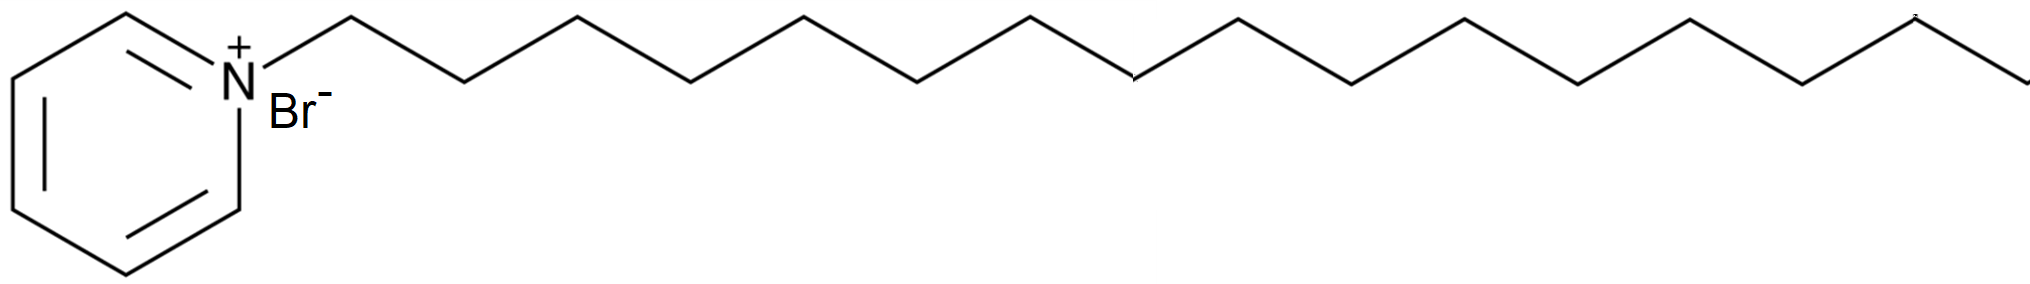
\includegraphics[width=0.8\textwidth]{assets/1019}
% 	\caption*{}
% \end{figure}} &
% \multirow{2}{*}{БЦП} & 0,1М & \textbf{139\textsuperscript{⁰}} &
% \begin{figure}[H]
% 	\centering
% 	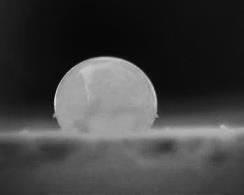
\includegraphics[width=0.8\textwidth]{assets/1020}
% 	\caption*{}
% \end{figure} \\
% & & 1 М & 128\textsuperscript{⁰} & нет изображения \\
% \multirow{2}{*}{\begin{figure}[H]
% 	\centering
% 	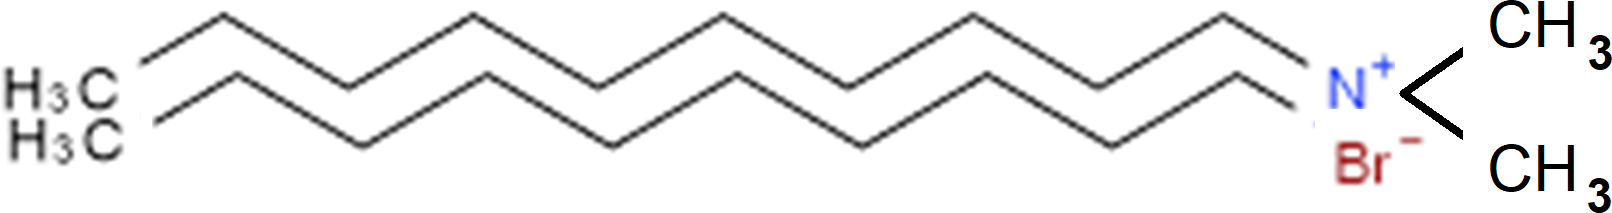
\includegraphics[width=0.8\textwidth]{assets/1021}
% 	\caption*{}
% \end{figure}} &
% \multirow{2}{*}{ДЦДMAБ} & 0,1М & 135\textsuperscript{⁰} & нет
% изображения \\
% & & 1 М & \textbf{161\textsuperscript{⁰}} &
% \begin{figure}[H]
% 	\centering
% 	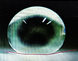
\includegraphics[width=0.8\textwidth]{assets/1022}
% 	\caption*{}
% \end{figure} \\
% \multirow{2}{*}{\begin{figure}[H]
% 	\centering
% 	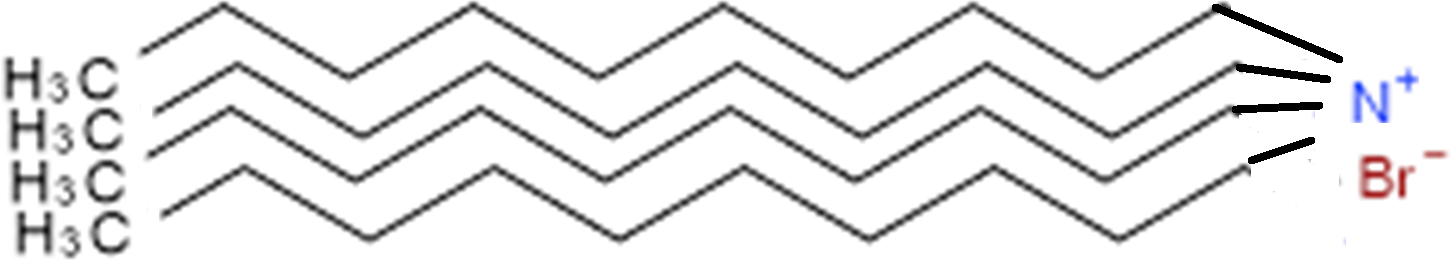
\includegraphics[width=0.8\textwidth]{assets/1023}
% 	\caption*{}
% \end{figure}} &
% \multirow{2}{*}{ТКБА} & 0,1М & 141\textsuperscript{⁰} & нет
% изображения \\
% & & 1 М & \textbf{170\textsuperscript{⁰}} &
% \begin{figure}[H]
% 	\centering
% 	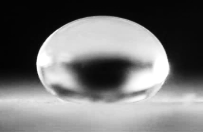
\includegraphics[width=0.8\textwidth]{assets/1024}
% 	\caption*{}
% \end{figure} \\
% \multirow{2}{*}{\begin{figure}[H]
% 	\centering
% 	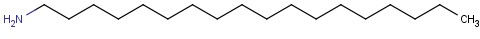
\includegraphics[width=0.8\textwidth]{assets/1025}
% 	\caption*{}
% \end{figure}}
% & \multirow{2}{*}{ОДА} & 0,1М & 131\textsuperscript{⁰} & нет
% изображения \\
% & & 1 М & \textbf{157\textsuperscript{⁰}} &
% \begin{figure}[H]
% 	\centering
% 	
\includegraphics[width=0.8\textwidth]{assets/1026}
% 	\caption*{}
% \end{figure}\textbf{9{]}} \\
% \end{longtable}

Среди органоглины, как указано в таблице 4, максимальный контактный угол
составил 170\textsuperscript{0} с ТКБА. Это можно объяснить структурой
молекулы ТКБА, т.е. молекула ТКБА имеет 4 длинные неполярные
углеводородные цепи, которые придают ей более гидрофобные свойства, чем
другим. Концевая сторона углеводорода ТКБА не имеет большого
пространства при плотной упаковке вместе, по сравнению с БЦП, молекула
БЦП имеет бензольное кольцо на концевой стороне, поэтому даже при самой
большой концентрации максимальное значение угла поглощения не превышало
128º.

Касательно остальных, то здесь наблюдается интересная ситуация (см.
табл. 4) при низкой концентрации гидрофобизатора (0.1 M), значения
контактных углов капель воды выше, чем при высоком значении концентрации
(1 M). В частности, в случае БЦП угол контакта уменьшился с 39º до 9º, в
случае ТМOДАБ - со 135º до 128º градусов. В других случаях, при
увеличении концентрации гидрофобизатора увеличивается и контактный угол
органоглины. Можно резюмировать, что данное снижение зависит от
особенностей этих молекул, то есть от положения и длины цепи, которую
молекула занимает на поверхности твердой частицы, что такое отклонение
произошло от слишком большой концентрации ПАВ. В результате молекула ПАВ
образует слой и происходит процесс обратной гидрофилизации поверхности
{[}36-42{]}, который показан на рис. 3:

\begin{figure}[H]
	\centering
	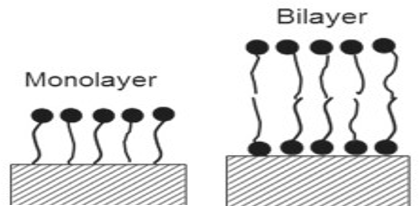
\includegraphics[width=0.8\textwidth]{assets/1027}
	\caption*{}
\end{figure}

\textbf{Рис. 3- Схематическое изображение самостоятельного
взаимодействия молекул ПАВ образуя двойной слой и обратную
гидрофилизации на поверхности частиц глин {[}30{]}}

\begin{figure}[H]
	\centering
	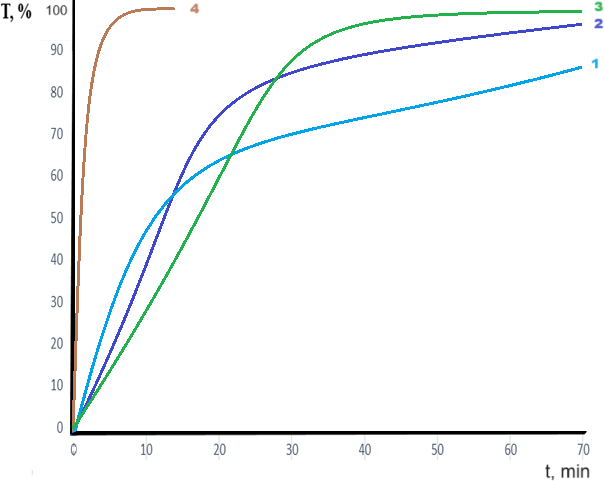
\includegraphics[width=0.8\textwidth]{assets/1028}
	\caption*{}
\end{figure}

\textbf{Рис. 4. - Кинетика седиментации частиц органоглины на основе
монтмориллонита в дизельном топливе, исследованная оптическим методом}

\textbf{1-ТКБА; 2-ДЦДMAБ; 3-БЦП; 4-TOДMAБ}

На рисунке 4 показано изменение оптически наблюдаемых значений
светопроводности суспензии органоглины, полученной с помощью различных
гидрофобизаторов, в дизтопливе в течение определенного времени.
Результаты показали, что органоглина, полученная в условиях присутствия
ТКБА, обладает наименьшим светопропусканием, а ее эквивалент составляет
82\%. В следующих исследованиях нами использовались органоглины с
наибольшим контактным углом. Было решено, что дальнейшие результаты
целесообразно продолжить с органоглиной, полученной только в присутствии
ТКБА, поскольку этот ПАВ оказался наиболее оптимальным
супергидрофобизатором.

На рисунке 5 показан результат спектрометрии на инфракрасном анализаторе
Фурье, который был получен для того, чтобы убедиться, что адсорбция ТКБА
была осуществлена на поверхности глины.

% \begin{longtable}[]{@{}
%   >{\raggedright\arraybackslash}p{(\columnwidth - 2\tabcolsep) * \real{0.5083}}
%   >{\raggedright\arraybackslash}p{(\columnwidth - 2\tabcolsep) * \real{0.4917}}@{}}
% \toprule\noalign{}
% \begin{minipage}[b]{\linewidth}\raggedright
% \end{minipage} & \begin{minipage}[b]{\linewidth}\raggedright
% \end{minipage} \\
% \midrule\noalign{}
% \endhead
% \bottomrule\noalign{}
% \endlastfoot
% \begin{figure}[H]
% 	\centering
% 	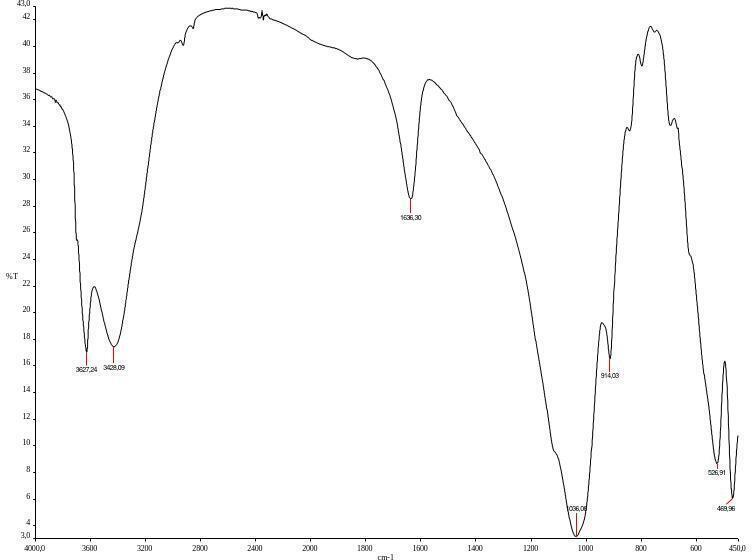
\includegraphics[width=0.8\textwidth]{assets/1029}
% 	\caption*{}
% \end{figure} &
% \begin{figure}[H]
% 	\centering
% 	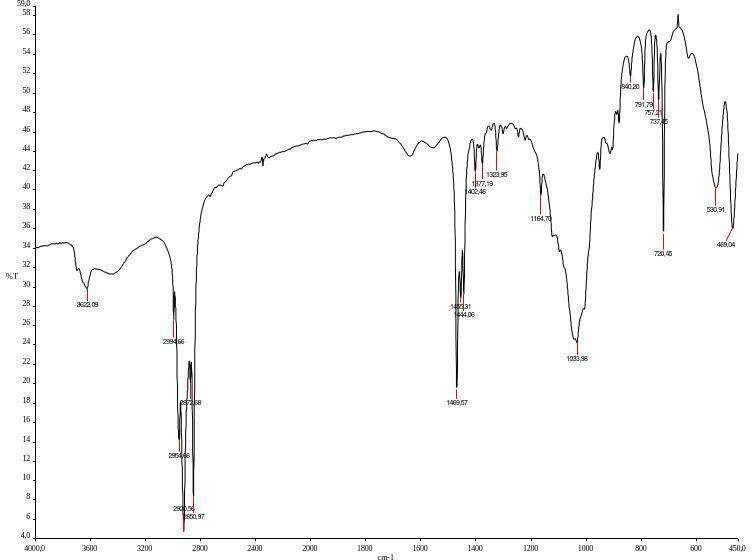
\includegraphics[width=0.8\textwidth]{assets/1030}
% 	\caption*{}
% \end{figure} \\
% \multicolumn{2}{@{}>{\raggedright\arraybackslash}p{(\columnwidth - 2\tabcolsep) * \real{1.0000} + 2\tabcolsep}@{}}{%
% а б
% 
% \textbf{Рис.5 - ИК-спектры (а) Na-монтмориллонита и (б)
% модифицированного}
% 
% \textbf{ТКБА органоглины}} \\
% \end{longtable}

Соответственно проведенные полосы и пики на инфракрасном анализаторе
Фурье указывают на интеркаляцию ПАВ в межслоевое пространство
монтмориллонита. В настоящее время ИК-спектроскопия является одним из
наиболее универсальных методов исследования твердого тела с помощью
компьютерных оптических методов, особенно тех, которые определяют
поверхностные группы атомов глинистого минерала и колебания элементов
его структуры, а также позволяют наблюдать изменения химических связей
при адсорбции реагентов. На рисунке 5 показаны колебания связей Si-O-Si,
наблюдаемые в широкой полосе, соответствующей 1036
см\textsuperscript{-1}. Пики по частоте 470.65 см\textsuperscript{-1} и
527 см\textsuperscript{-1} отражают колебания связи Me-O. Пики с
частотой 914 см-1 определяют колебания связей Si-О-Si. Пики в интервалах
3100-3500 см\textsuperscript{-1} (практически 3627
см\textsuperscript{-1}) молекул связаной воды в молекуле
монтмориллонита, а колебания пика при 1631 см\textsuperscript{-1}
показывают деформационные колебания, отражающие водородную связь.

В диапазоне частот 1444-1469 см\textsuperscript{-1} присутствуют пики,
которые указывают на связи C-H. Пики на 2850,97 см\textsuperscript{-1},
2954 см\textsuperscript{-1}\textsubscript{,} 2872,68
см\textsuperscript{-1}\textsubscript{,} 2994,66 см\textsuperscript{-1} и
2920,0 см\textsuperscript{-1} - показывают колебания
CH\textsubscript{2}-связей. Итак, мы убедились, что адсорбция ТКБА на
поверхности монтмориллонита происходит.

\begin{figure}[H]
	\centering
	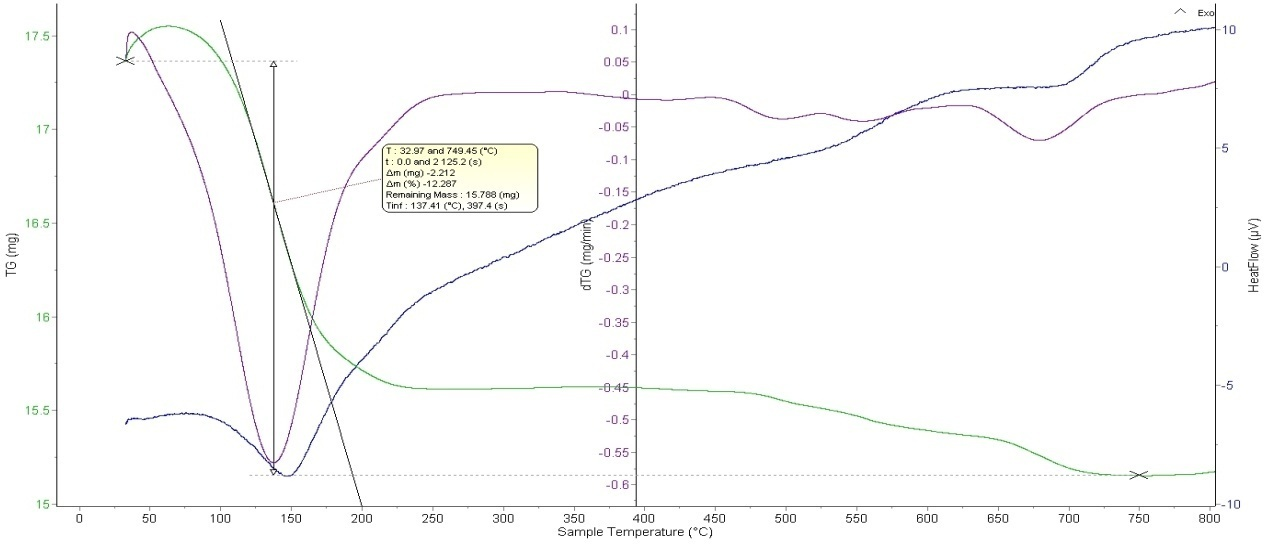
\includegraphics[width=0.8\textwidth]{assets/1031}
	\caption*{}
\end{figure}

\textbf{Рис. 6. - Результаты ДСК и ТГА анализа для Na - монтмориллонита}

Данный анализ показывает, что при увеличении температуры от 140 ⁰ Cдо
200 ⁰ C масса исследуемого объекта уменьшается. Это показывает, что
здесь происходят различные межфазные изменения (зеленая кривая). В ходе
процесса было замечено, что при повышении температуры масса уменьшается,
то есть видно, что состав начинает отделяться от содержащегося в нем
количества воды и переходить в кристаллическую форму {[}31{]}. Было
замечено, что изменение массы замедлилось на 15,788 мг. Как мы можем
видеть, температура плавления менялась (фиолетовая кривая).

\begin{figure}[H]
	\centering
	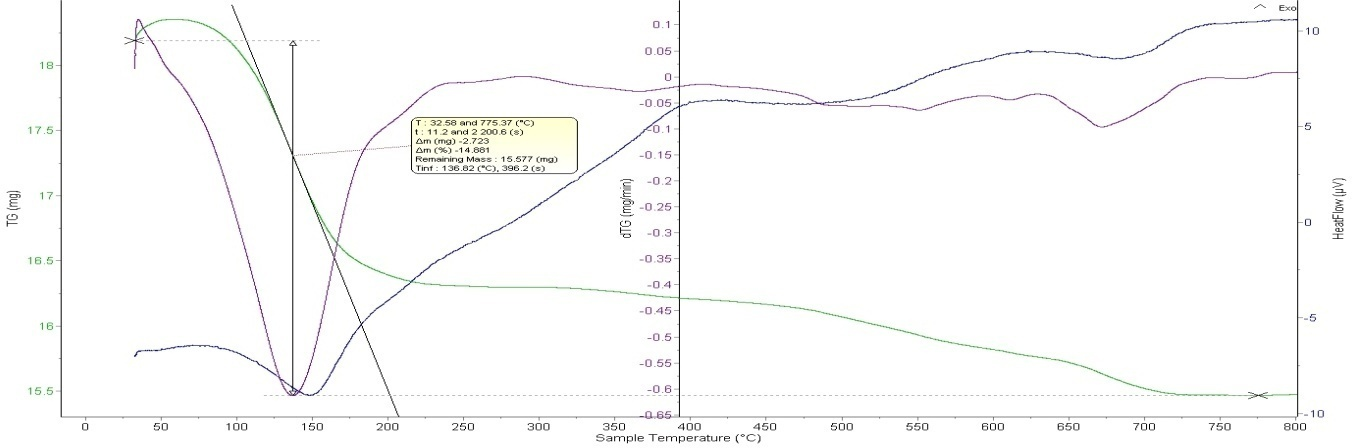
\includegraphics[width=0.8\textwidth]{assets/1032}
	\caption*{}
\end{figure}

\textbf{Рис. 7- Анализ ДСК и ТГА органоглины, полученной в условиях
наличия ТКБА}

Наблюдаются те же явления, но потеря массы органоглины, полученной ТКБА,
происходит активнее, то есть углеводородная цепь, входящая в состав
ТКБА, окисляется в присутствии кислорода, расщепляется и улетает в виде
газа СО\textsubscript{2}. В ходе эксперимента, было замечено, что
изменение массы органоглины, полученной ТКБА замедлилось до 15 577 мг.

\textbf{Выводы.}

\begin{enumerate}
\def\labelenumi{\arabic{enumi}.}
\item
  Из бентонита местрождения «Таганское» Восточно-Казахстанской области
  были разработаны четыре типа органоглин при различных концентрациях
  катионных ПАВ-- 1-ТКБА; 2-ДЦДMAБ; 3-ЦПБ; 4-TOДMAБ.
\item
  Было выполнено измерение контактного угла с помощью капли воды на
  поверхности полученных органофильных глинопорошков, при этом было
  обнаружено, что при высокой концентрации ТКБА контактный угол капли
  воды равен 170º, а в присутствии других концентраций ТКБА контактный
  угол был равен всего 140º.
\item
  Изучены устойчивости органофильных глин в органической среде
  оптическим методом и самой оптимальной оказалась супергидрофобная
  глина, полученная с помощью ТКБА, мутность которой была равна 82\%.
\item
  В ходе исследований была разработана технологическая схема получения
  органоглины, был установлен способ и определена методика получения
  модифицированной органоглины с ТКБА.
\end{enumerate}

\emph{\textbf{Финансирование.} Данное научное исследование проводилось в
рамках грантового финансирования проекта ИРН AP19674742 «Технология
получения нового органоминерального композиционного материала на основе
природного бентонита Восточного Казахстана». Источник финансирования -
Комитет науки Министерства науки и высшего образования Республики
Казахстан.}

Авторы выражают благодарность за выделенное грантовое финансирование.

\textbf{Литература}

1. Ianchis R., Donescu D., Cinteza L.O.~et al\emph{.}~Polymer-clay
nanocomposites obtained by solution polymerization of vinyl benzyl
triammonium chloride in the presence of advanced functionalized clay
//J. Chem Sc.~-2014. -Vol.126. - P.609--616.
https://doi.org/10.1007/s12039-014-0621-0

2. Hodhaifa D., Meghabar R., Benachour M.~et al\emph{.}~Polymer-Clay
Nanocomposites: Exfoliation and Intercalation of Organophilic
Montmorillonite Nanofillers in Styrene--Limonene Copolymer //~Polym.
Sci. Ser\emph{. -}2021.-Vol.~63.- P.568--575.
https://doi.org/10.1134/S0965545X21050023

3. Mehri S., Ahmadinejad N., Akbarzadeh A. Vinyl Modified Cloisite 30B
Clay as an Efficient Filler for the Synthesis of
Poly(styrene-\emph{co}-butyl acrylate)/Clay Nanocomposite by Emulsion
Polymerization //Polym. Sci. Ser.- 2019.-Vol.61.-P.493-502

https://doi.org/10.1134/S1560090419040043

4. Zare Y., Fasihi M., Rhee K. Y. Efficiency of stress transfer between
polymer matrix and nanoplatelets in clay/polymer nanocomposites
//~Applied Clay Science.~ -2017. -Vol.143.-P. 265-272
https://doi.org/10.1016/j.clay.2017.03.043

5. Guanzheng Zh., Zepeng Zh., Maguy J. Organoclays used as colloidal and
rheological additives in oil-based drilling fluids: An overview//
Applied Clay Science. -2019.-Vol.177.-P.63-81,
https://doi.org/10.1016/j.clay.2019.05.006

6. Rogers K., Takács E., Thompson M. Contact angle measurement of select
compatibilizers for polymer-silicate layer nanocomposites //Polimer
Testing.-2005.-Vol.24.- P.423-427. https://doi.org/10.1016/
j.polymertesting.2005.01.010

7. Pegoretti A., Dorigato A., Brugnara M., Penati, A. Contact angle
measurements as a tool to investigate the filler--matrix interactions in
polyurethane--clay nanocomposites from blocked prepolymer// European
Polymer Journal. -2008. -Vol. 44(6). - P.1662-1672.~

https://doi.org/10.1016/j.eurpolymj.2008.04.011

8. Elias E., Chandran C. S., Chandran N., Souza F. G., Thomas
S.~Segmental dynamics, morphology and thermomechanical properties of
electrospun poly(ε-caprolactone) nanofibers in the presence of an
interacting filler // RSC Advances.-2016. -Vol.6(26).-
P.21376--21386.~https://doi.org/10.1039/c5ra24251g

9. Musabekov K.B., Artykova D.M-K., Tazhibayeva S.M., Oryntaeva A.,
Sugurbekova G.K., Kulichikhin V. Surface modification of montmorillonite
clay with organic molecules // Rasayan J. Chem.-
2021.-Vol.14(1).-P.635-640. http://dx.doi.org/10.31788/RJC.2021.1416093

10. Hadj-Hamou A.S., Metref F., Yahiaoui F. Thermal stability and
decomposition kinetic studies of antimicrobial PCL/nanoclay packaging
films //~Polym. Bull.-
2017.-Vol.74.-P.3833--3853.~https://doi.org/10.1007/s00289-017-1929-y

11. Kurmangazhi G., Tazhibayeva S. M.,~ Musabekov K. B.,~ Levin I. S.,~
Kuzin M. S.,~ Ermakova L. E.,~~Yu V. K.~ Preparation of Dispersed
Magnetite--Bentonite Composites and Kazcaine Adsorption on Them
//~Colloid J.-~2021. -Vol.83.- P.343-351.

https://doi.org/10.1134/S1061933X21030091

12.
https://www.sigmaaldrich.com/KZ/en/products/chemistry-and-biochemicals/lab-chemicals-
Date of address:12.02.2024

13. https://www.facebook.com/kjickaznau/- Date of address:12.02.2024

14. https://www.openscience.ru/chem/index.php?page=wetting\&item=003-

Date of address:16.02.2024

15. https://fundamental-research.ru/ru/article/view?id=3212- Date of
address:16.02.2024

16. Cailun W., Myshkin V.E., Bespala E.V., Poberezhnikov А.D., Baraban
А.P., Shukshina D.D., Semenov D.А. Structure and properties of
montmorillonite containing Ca\textsuperscript{2+},
Sr\textsuperscript{2+}, and Ba\textsuperscript{2+}~cations
simultaneously // Journal of Molecular Liquids. -2023. -Vol. 382. -
121994.

https://doi.org/10.1016/j.molliq.2023.121994

17.Brigatti M. F., Galan E., Theng B. K. G. Chapter 2 Structures and
Mineralogy of Clay Minerals// Developments of Clay Science. -2006.
-Vol.1.- P.9 - 86.~

https://doi.org/10.1016/s1572-4352(05)01002-0

18. Peng J., Yi H., Song S., Zhan W., Zhao Y. Driving force for the
swelling of montmorillonite as affected by surface charge and
exchangeable cations: A molecular dynamic study// Results in Physics.
-2019. -Vol.12.- P.113-117.~https://doi.org/10.1016/j.rinp.2018.11.011

19. Ngouana BFW, Kalinichev AG. Structural arrangements of isomorphic
substitutions in smectites: Molecular simulation of the swelling
properties, interlayer structure, and dynamics of hydrated
Cs-montmorillonite revisited with new clay models //J. Phys. Chem. C.
-2014. -Vol.118. -P.12758-12773. https://doi.org/10.1021/jp500538z

20.Xian Z, Hao Y, Zhao Y, Song S. Quantitative determination of
isomorphous substitutions on clay mineral surfaces through AFM imaging:
a case of mica // Colloids and Surf. A Physicochem and Eng. Asp. -2017.
-Vol.533.- P.55-60. https://doi.org/10.1016/j.colsurfa.2017.08.024

21. Zhao Y, Yi H, Jia F, Li H, Peng C, Song S. A novel method for
determining the thickness of hydration shells on nanosheets: a case of
montmorillonite in water //Powder Technol. -2017. -Vol.306.- P.74 -79.
https://doi.org/10.1016/j.powtec.2016.10.045

22. Ferrage E, Lanson B, Sakharov BA, Drits VA. Investigation of
smectite hydration properties by modeling experimental X-ray diffraction
patterns: Part I: Montmorillonite hydration properties //Amertcan
Mineral. -2005. -Vol.90.- P.1358--1374.
https://doi.org/10.2138/am.2005.1776

23. Zhang L, Lu X, Liu X, Zhou J, Zhou H. Hydration and Mobility of
Interlayer Ions of (Na\textsubscript{x},
Ca\textsubscript{y})-Montmorillonite: A Molecular Dynamics Study // J.
Phys. Chem. C. -2014.-Vol.118. --P.29811-29821.
https://doi.org/10.1021/jp508427c

24. Salles F., Bildstein O., Douillard J.M., Jullien M., Van Damme H.
Determination of the Driving Force for the Hydration of the Swelling
Clays from Computation of the Hydration Energy of the Interlayer Cations
and the Clay Layer // J. Phys. Chem. C. -2007. -Vol.111.-
P.13170--13176. https://doi.org/10.1021/jp0719762.

25.Emmerich K, Koeniger F, Kaden H, Thissen P. Microscopic structure and
properties of discrete water layer in Na-exchanged montmorillonite // J.
Colloid Interface Sc. -2015.-Vol.448.- P.24--31.
https://doi.org/10.1016/j.jcis.2015.01.087

26. Edwin R., Eddy D., Iman S., Iman R. The organic modification of
pre-lithiated montmorillonite //Rassayan J.Chem.-2022. -Special Issue.-
P.167-171.

https://doi.org/. 10.31788/RJC.2022.1558226

27. Fomina М., Skorochod I. Microbial Interaction with Clay Minerals and
Its Environmental and Biotechnological Implication//~ Minerals. -2020.-
Vol.10(10).- P.861.

https://doi.org/10.3390/min10100861

28. Bibi I., Icenhower J., Niazi N.K., Naz T., Shahid M., Bashir S.
Chapter 21~-~Clay Minerals:~Structure, Chemistry, and Significance in
Contaminated Environments and Geological
CO\textsubscript{2}~Sequestration. //Environmetal Materials and Waste.-
2016. - P.543-567

https://doi.org/10.1016/B978-0-12-803837-6.00021-4

29. Roshin Р., Sreelekshmi R.V., Menon А.R. Cetyltrimethyl Ammonium
Bromide Modified Kaolin as a Reinforcing Filler for Natural Rubber //~J.
Polym. Environ. -2018.-Vol.~26.- P.39--47.
https://doi.org/10.1007/s10924-016-0915-z

30. Chuan~C.~,~Jingong~C.,~Huiming~L.,~Xuejun~W.,~Xiang~Z.,~Yongshi~W.
Occurrence of organic matter in argillaceous sediments and rocks and its
geological significance: A review//Chemical Geology. -2023. -Vol. 639.
-121737. https://doi.org/10.1016/j.chemgeo.2023.121737

31. Shi, L., Huang, J., Zeng, G.~et al.~ Roles of surfactants in
pressure-driven membrane separation processes: a review //Environ Sci
Pollut Res. -2019. -Vol.26.- P. 30731-30754.

https://doi.org/10.1007/s11356-019-06345-x

32.Zhiping~S.,~Pengxiang~L.,~Liyan~L. Interactions between CTAB and
montmorillonite by atomic force microscopy and molecular dynamics
simulation //Colloids and Surfaces A: Physicochemical and Engineering
Aspects. -2023. -Vol.657. Part B.-P.130656.

https://doi.org/10.1016/j.colsurfa.2022.130656

33. Ibraimova D. M-K., Rozhkova O.V., Musabekov K.B., Tazhibayeva S.M.,
Rozhkov V., Yermekov M.T. Development of Methods to Obtain Composite
Materials from Organoclays //Eurasian Journal of Chemistry. -2023.
-Vol.4(112). -- P.101-111. https://doi.org/10.31489/2959-0663/4-23-14

34.Musabekov K.B., Zhakyp B., Tazhibayeva S.M., Musabekov N., Ergaliyeva
A. A research of colloidal silver immobilization in bionanocomposites of
natural polymers and montmorillonite// Eastern-European J.of Enterprise
Technologies. -2020.

-Vol.6 (108).- P.93-101.
http://dx.doi.org/10.15587/1729-4061.2020.216995

35. Рожкова О.В., Муздыбаева Ш.А., Мусабеков К.Б., Ибраимова Д. М.,
Рожков В.И., Ермеков М.Т. Разработка методов получения носителей
лекарственных средств на основе органомодифицированных глин // Известия
Национальной академии наук Республики Казахстан. Серия химических наук.
-2023 -№ 3.- C.138-156.

https://doi.org/10.32014/2023.2518-1491.183

36.Musabekov K.B., Rozhkova O.V., Artykova (Ibraimova) D. M-K., Yermekov
M.T., Muzdybaeva Sh.A. Application of bentonite clay as a protective
barrier in the disposal of radioactive waste of nuclear industry of
kazakhstan // News of the national Academy of sciences og the republic
of Kazakhstan. Series Chemistry and Technology. -2023. -№ 1.- S.66-77.

https://doi.org/10.32014/2023.2518-1491.148

37. Askapova B., Musabekov K.B. Modification of bentonites inoculation
with iron compounds to afford magnetite clays //~Studia UBB CHEMIA.LXVII
-2022.-Vol.2.-P.131-141.~https://doi.org/10.24193/subbchem.2022.2.08

38. Tyussyupova B., Tazhibayeva S.M., Musabekov K., Mussatay Y.,
Kokanbaev A. Effect of Proteolytic Enzymes on The Biological
Degradability of Gelatin-Based Films // International J. of Engineering
Res. and Technology.~-2020.-Vol.13.-№11- P.3699--3704.

https://dx.doi.org/10.37624/IJERT/13.11.2020.3699-3704

39. Аtyaksheva~ А., Рожкова О.В., Sarsikeyev Y., Аtyaksheva~ А.,
Yermekov M.T., Smagulov А., Ryvkina N. Determination of rational
parameters for heat treatment of concrete mixture based on a hollow
aluminosilicate microsphere //Eastern-European J.of Enterprise
Technologies. -2022. -Vol.1. -№ 6(115).- P.64-72.
https://doi.org/10.15587/1729-4061.2022.251004

40. Ermekov M., Rozhkova O., Sandibekova S.G., Belenko E.V., Tolysbaev
T., Vetjugov A., Turbin O. A., Belenko E. V. Storage of the industrial
waste of the mining and smelting industry of Kazakhstan, landfills
arrangement,efficiency and operational features// News of the national
Academy of sciences og the republic of Kazakhstan. Series of geology and
technical sciences.- 2020. - № 6(444).- S.83-89.
https://doi.org/10.32014/2020.2518-170X.134.

41. Musabekov К., Zhakyp B., Tazhibayeva S., ~Musabekov N., Yergaliyeva
А. A research of colloidal silver immobilization in bionanocomposites of
natural polymers and montmorillonite // Eastern-European Journal of
Enterprise Technologies.- 2020.-Vol.6(6--108).- S.93--101.
https://doi.org/10.15587/1729-4061.2020.216995

42. Yerlan G.Ye., Tyussyupova B.B., Tazhibayeva S.M., Musabekov K.B.,
Balabushevich N.G., Kokanbayev A.K. Encapsulation of Insulin in
Biodegradable Polymers //Eurasian Chemico-Technological J. -2022.
-Vol.24.- P.351-361. https://doi.org/10.18321/ectj1479

\textbf{References}

1. Ianchis R., Donescu D., Cinteza L.O.~et al\emph{.}~Polymer-clay
nanocomposites obtained by solution polymerization of vinyl benzyl
triammonium chloride in the presence of advanced functionalized clay
//J. Chem Sc.~-2014. -Vol.126. - P.609--616.
https://doi.org/10.1007/s12039-014-0621-0

2. Hodhaifa D., Meghabar R., Benachour M.~et al\emph{.}~Polymer-Clay
Nanocomposites: Exfoliation and Intercalation of Organophilic
Montmorillonite Nanofillers in Styrene--Limonene Copolymer //~Polym.
Sci. Ser\emph{. -}2021.-Vol.~63.- P.568--575.
https://doi.org/10.1134/S0965545X21050023

3. Mehri S., Ahmadinejad N., Akbarzadeh A. Vinyl Modified Cloisite 30B
Clay as an Efficient Filler for the Synthesis of
Poly(styrene-\emph{co}-butyl acrylate)/Clay Nanocomposite by Emulsion
Polymerization //Polym. Sci. Ser.- 2019.-Vol.61.-P.493-502

https://doi.org/10.1134/S1560090419040043

4. Zare Y., Fasihi M., Rhee K. Y. Efficiency of stress transfer between
polymer matrix and nanoplatelets in clay/polymer nanocomposites
//~Applied Clay Science.~ -2017. -Vol.143.-P. 265-272
https://doi.org/10.1016/j.clay.2017.03.043

5. Guanzheng Zh., Zepeng Zh., Maguy J. Organoclays used as colloidal and
rheological additives in oil-based drilling fluids: An overview//
Applied Clay Science. -2019.-Vol.177.-P.63-81,
https://doi.org/10.1016/j.clay.2019.05.006

6. Rogers K., Takács E., Thompson M. Contact angle measurement of select
compatibilizers for polymer-silicate layer nanocomposites //Polimer
Testing.-2005.-Vol.24.- P.423-427. https://doi.org/10.1016/
j.polymertesting.2005.01.010

7. Pegoretti A., Dorigato A., Brugnara M., Penati, A. Contact angle
measurements as a tool to investigate the filler--matrix interactions in
polyurethane--clay nanocomposites from blocked prepolymer// European
Polymer Journal. -2008. -Vol. 44(6). - P.1662-1672.~

https://doi.org/10.1016/j.eurpolymj.2008.04.011

8. Elias E., Chandran C. S., Chandran N., Souza F. G., Thomas
S.~Segmental dynamics, morphology and thermomechanical properties of
electrospun poly(ε-caprolactone) nanofibers in the presence of an
interacting filler // RSC Advances.-2016. -Vol.6(26).-
P.21376--21386.~https://doi.org/10.1039/c5ra24251g

9. Musabekov K.B., Artykova D.M-K., Tazhibayeva S.M., Oryntaeva A.,
Sugurbekova G.K., Kulichikhin V. Surface modification of montmorillonite
clay with organic molecules // Rasayan J. Chem.-
2021.-Vol.14(1).-P.635-640. http://dx.doi.org/10.31788/RJC.2021.1416093

10. Hadj-Hamou A.S., Metref F., Yahiaoui F. Thermal stability and
decomposition kinetic studies of antimicrobial PCL/nanoclay packaging
films //~Polym. Bull.-
2017.-Vol.74.-P.3833--3853.~https://doi.org/10.1007/s00289-017-1929-y

11. Kurmangazhi G., Tazhibayeva S. M.,~ Musabekov K. B.,~ Levin I. S.,~
Kuzin M. S.,~ Ermakova L. E.,~~Yu V. K.~ Preparation of Dispersed
Magnetite--Bentonite Composites and Kazcaine Adsorption on Them
//~Colloid J.-~2021. -Vol.83.- P.343-351.

https://doi.org/10.1134/S1061933X21030091

12.
https://www.sigmaaldrich.com/KZ/en/products/chemistry-and-biochemicals/lab-chemicals-
Date of address:12.02.2024

13. https://www.facebook.com/kjickaznau/- Date of address:12.02.2024

14. https://www.openscience.ru/chem/index.php?page=wetting\&item=003-

Date of address:16.02.2024

15. https://fundamental-research.ru/ru/article/view?id=32127- Date of
address:16.02.2024

16. Cailun W., Myshkin V.E., Bespala E.V., Poberezhnikov А.D., Baraban
А.P., Shukshina D.D., Semenov D.А. Structure and properties of
montmorillonite containing Ca\textsuperscript{2+},
Sr\textsuperscript{2+}, and Ba\textsuperscript{2+}~cations
simultaneously // Journal of Molecular Liquids. -2023. -Vol. 382. -
121994.

https://doi.org/10.1016/j.molliq.2023.121994

17.Brigatti M. F., Galan E., Theng B. K. G. Chapter 2 Structures and
Mineralogy of Clay Minerals// Developments of Clay Science. -2006.
-Vol.1.- P.9 - 86.~

https://doi.org/10.1016/s1572-4352(05)01002-0

18. Peng J., Yi H., Song S., Zhan W., Zhao Y. Driving force for the
swelling of montmorillonite as affected by surface charge and
exchangeable cations: A molecular dynamic study// Results in Physics.
-2019. -Vol.12.- P.113-117.~https://doi.org/10.1016/j.rinp.2018.11.011

19. Ngouana BFW, Kalinichev AG. Structural arrangements of isomorphic
substitutions in smectites: Molecular simulation of the swelling
properties, interlayer structure, and dynamics of hydrated
Cs-montmorillonite revisited with new clay models //J. Phys. Chem. C.
-2014. -Vol.118. -P.12758-12773. https://doi.org/10.1021/jp500538z

20.Xian Z, Hao Y, Zhao Y, Song S. Quantitative determination of
isomorphous substitutions on clay mineral surfaces through AFM imaging:
a case of mica // Colloids and Surf. A Physicochem and Eng. Asp. -2017.
-Vol.533.- P.55-60. https://doi.org/10.1016/j.colsurfa.2017.08.024

21. Zhao Y, Yi H, Jia F, Li H, Peng C, Song S. A novel method for
determining the thickness of hydration shells on nanosheets: a case of
montmorillonite in water //Powder Technol. -2017. -Vol.306.- P.74 -79.
https://doi.org/10.1016/j.powtec.2016.10.045

22. Ferrage E, Lanson B, Sakharov BA, Drits VA. Investigation of
smectite hydration properties by modeling experimental X-ray diffraction
patterns: Part I: Montmorillonite hydration properties //Amertcan
Mineral. -2005. -Vol.90.- P.1358--1374.
https://doi.org/10.2138/am.2005.1776

23. Zhang L, Lu X, Liu X, Zhou J, Zhou H. Hydration and Mobility of
Interlayer Ions of (Na\textsubscript{x},
Ca\textsubscript{y})-Montmorillonite: A Molecular Dynamics Study // J.
Phys. Chem. C. -2014.-Vol.118. --P.29811-29821.
https://doi.org/10.1021/jp508427c

24. Salles F., Bildstein O., Douillard J.M., Jullien M., Van Damme H.
Determination of the Driving Force for the Hydration of the Swelling
Clays from Computation of the Hydration Energy of the Interlayer Cations
and the Clay Layer // J. Phys. Chem. C. -2007. -Vol.111.-
P.13170--13176. https://doi.org/10.1021/jp0719762.

25.Emmerich K, Koeniger F, Kaden H, Thissen P. Microscopic structure and
properties of discrete water layer in Na-exchanged montmorillonite // J.
Colloid Interface Sc. -2015.-Vol.448.- P.24--31.
https://doi.org/10.1016/j.jcis.2015.01.087

26. Edwin R., Eddy D., Iman S., Iman R. The organic modification of
pre-lithiated montmorillonite //Rassayan J.Chem.-2022. -Special Issue.-
P.167-171.

https://doi.org/. 10.31788/RJC.2022.1558226

27. Fomina М., Skorochod I. Microbial Interaction with Clay Minerals and
Its Environmental and Biotechnological Implication//~ Minerals. -2020.-
Vol.10(10).- P.861.

https://doi.org/10.3390/min10100861

28. Bibi I., Icenhower J., Niazi N.K., Naz T., Shahid M., Bashir S.
Chapter 21~-~Clay Minerals:~Structure, Chemistry, and Significance in
Contaminated Environments and Geological
CO\textsubscript{2}~Sequestration. //Environmetal Materials and Waste.-
2016. - P.543-567

https://doi.org/10.1016/B978-0-12-803837-6.00021-4

29. Roshin Р., Sreelekshmi R.V., Menon А.R. Cetyltrimethyl Ammonium
Bromide Modified Kaolin as a Reinforcing Filler for Natural Rubber //~J.
Polym. Environ. -2018.-Vol.~26.- P.39--47.
https://doi.org/10.1007/s10924-016-0915-z

30. Chuan~C.~,~Jingong~C.,~Huiming~L.,~Xuejun~W.,~Xiang~Z.,~Yongshi~W.
Occurrence of organic matter in argillaceous sediments and rocks and its
geological significance: A review//Chemical Geology. -2023. -Vol. 639.
-121737. https://doi.org/10.1016/j.chemgeo.2023.121737

31. Shi, L., Huang, J., Zeng, G.~et al.~ Roles of surfactants in
pressure-driven membrane separation processes: a review //Environ Sci
Pollut Res. -2019. -Vol.26.- P. 30731-30754.

https://doi.org/10.1007/s11356-019-06345-x

32.Zhiping~S.,~Pengxiang~L.,~Liyan~L. Interactions between CTAB and
montmorillonite by atomic force microscopy and molecular dynamics
simulation //Colloids and Surfaces A: Physicochemical and Engineering
Aspects. -2023. -Vol.657. Part B.-P.130656.

https://doi.org/10.1016/j.colsurfa.2022.130656

33. Ibraimova D. M-K., Rozhkova O.V., Musabekov K.B., Tazhibayeva S.M.,
Rozhkov V., Yermekov M.T. Development of Methods to Obtain Composite
Materials from Organoclays //Eurasian Journal of Chemistry. -2023.
-Vol.4(112). -- P.101-111. https://doi.org/10.31489/2959-0663/4-23-14

34.Musabekov K.B., Zhakyp B., Tazhibayeva S.M., Musabekov N., Ergaliyeva
A. A research of colloidal silver immobilization in bionanocomposites of
natural polymers and montmorillonite// Eastern-European J.of Enterprise
Technologies. -2020.

-Vol.6 (108).- P.93-101.
http://dx.doi.org/10.15587/1729-4061.2020.216995

35. Rozhkova O.V., Muzdybaeva Sh.A., Musabekov K.B., Ibraimova D. M.,
Rozhkov V.I., Ermekov M.T. Razrabotka metodov poluchenija nositelej
lekarstvennyh sredstv na osnove organomodificirovannyh glin // Izvestija
Nacional\textquotesingle noj akademii nauk Respubliki Kazahstan. Serija
himicheskih nauk. -2023 -№ 3.- S.138-156. {[}in Russian{]}

https://doi.org/10.32014/2023.2518-1491.183

36.Musabekov K.B., Rozhkova O.V., Artykova (Ibraimova) D. M-K., Yermekov
M.T., Muzdybaeva Sh.A. Application of bentonite clay as a protective
barrier in the disposal of radioactive waste of nuclear industry of
kazakhstan // News of the national Academy of sciences og the republic
of Kazakhstan. Series Chemistry and Technology. -2023. -№ 1.- S.66-77.

https://doi.org/10.32014/2023.2518-1491.148.

37. Askapova B., Musabekov K.B. Modification of bentonites inoculation
with iron compounds to afford magnetite clays //~Studia UBB CHEMIA.LXVII
-2022.-Vol.2.-P.131-141.~https://doi.org/10.24193/subbchem.2022.2.08

38. Tyussyupova B., Tazhibayeva S.M., Musabekov K., Mussatay Y.,
Kokanbaev A. Effect of Proteolytic Enzymes on The Biological
Degradability of Gelatin-Based Films // International J. of Engineering
Res. and Technology.~-2020.-Vol.13.-№11- P.3699--3704.

https://dx.doi.org/10.37624/IJERT/13.11.2020.3699-3704

39. Аtyaksheva~ А., Рожкова О.В., Sarsikeyev Y., Аtyaksheva~ А.,
Yermekov M.T., Smagulov А., Ryvkina N. Determination of rational
parameters for heat treatment of concrete mixture based on a hollow
aluminosilicate microsphere //Eastern-European J.of Enterprise
Technologies. -2022. -Vol.1. -№ 6(115).- P.64-72.
https://doi.org/10.15587/1729-4061.2022.251004

40. Ermekov M., Rozhkova O., Sandibekova S.G., Belenko E.V., Tolysbaev
T., Vetjugov A., Turbin O. A., Belenko E. V. Storage of the industrial
waste of the mining and smelting industry of Kazakhstan, landfills
arrangement,efficiency and operational features// News of the national
Academy of sciences og the republic of Kazakhstan. Series of geology and
technical sciences.- 2020. - № 6(444).- S.83-89.
https://doi.org/10.32014/2020.2518-170X.134

N E W S

OF THE ACADEMY OF SCIENCES

OF THE REPUBLIC OF KAZAKHSTAN

N E W S

OF THE NATIONAL ACADEMY OF SCIENCES OF THE REPUBLIC OF KAZAKHSTAN

SERIES OF GEOLOGY AND TECHNICAL SCIENCES

N E W S

OF THE NATIONAL ACADEMY OF SCIENCES OF THE REPUBLIC OF KAZAKHSTAN

SERIES OF GEOLOGY AND TECHNICAL SCIENCES

N E W S

OF THE NATIONAL ACADEMY OF SCIENCES OF THE REPUBLIC OF KAZAKHSTAN

SERIES OF GEOLOGY AND TECHNICAL SCIENCES

N E W S

OF THE NATIONAL ACADEMY OF SCIENCES OF THE REPUBLIC OF KAZAKHSTAN

SERIES OF GEOLOGY AND TECHNICAL SCIENCES

41. Musabekov К., Zhakyp B., Tazhibayeva S., ~Musabekov N., Yergaliyeva
А. A research of colloidal silver immobilization in bionanocomposites of
natural polymers and montmorillonite //

Eastern-European Journal of Enterprise
Technologies.-2020.-Vol.6(6--108).- S.93--101.
https://doi.org/10.15587/1729-4061.2020.216995

42. Yerlan G.Ye., Tyussyupova B.B., Tazhibayeva S.M., Musabekov K.B.,
Balabushevich N.G., Kokanbayev A.K. Encapsulation of Insulin in
Biodegradable Polymers //Eurasian Chemico-Technological J. -2022.
-Vol.24.- P.351-361. https://doi.org/10.18321/ectj1479

\emph{\textbf{Сведения об авторах}}

Рожкова О.В. - доктор химических наук, профессор, академик Национальной
академии естественных наук Республики Казахстан, НАО «Казахский
агротехнический исследовательский университет имени Сакена Сейфуллина»,
Астана, Казахстан, АО «Science and Technology Solutions», Алматы,
Казахстан, e-mail: rozhkova.o@stsolutions.kz;

Ибраимова Д.М-К. - кандидат химических наук, старший преподаватель НАО
«Казахский национальный университет имени аль-Фараби», Алматы,
Казахстан,e-mail: dana\_kereevna@kaznu.kz;

Рожков В.И. - кандидат технических наук, НАО «Казахский агротехнический
университет имени Сакена Сейфуллина», Астана, Казахстан, ТОО «Алтайский
геолого-экологический институт», Усть-Каменогорск, Казахстан, e-mail:
vitalrza1983@gmail.com;

Ермеков М.Т.- Директор Департамента проектов и управления активами АО
«Science and Technology olutions», Алматы, Казахстан, e-mail:
yermekov.m@stsolutions.kz;

Кудайбергенова С.Ж. - кандидат химических наук, НАО «Казахский
агротехнический университет имени Сакена Сейфуллина», Астана, Казахстан,
e-mail: ksg.75.75@mail.ru;

Букеева А.Б. - кандидат химических наук, НАО «Казахский агротехнический
- кандидат химических наук, НАО «Казахский агротехнический университет
имени Сакена Сейфуллина», Астана, Казахстан, e-mail: akbota712@mail.ru;

Нуртай Ж.Т. - PhD, ассоциированный профессор Казахский Университет
технологии и бизнеса им К.Кулажанова Астана, Казахстан, e-mail:
zhadira\_nurtai@mail.ru

\emph{\textbf{Information about the authors}}

Rozhkova O.V. - Doctor of Natural Sciences, Professor, Academician of
the National Academy of Sciences of the Republic of Kazakhstan, NJSC
"Kazakh Agrotechnical Research University named after Saken Seifullin",
Astana, Kazakhstan, JSC "Science and Technology Solutions", Almaty,
Kazakhstan, e-mail: rozhkova.o@stsolutions.kz;

Ibraimova D.M-K. - Candidate of Chemical Sciences, senior lecturer at
Al-Farabi Kazakh National University, Almaty, Kazakhstan, e-mail:
dana\_kereevna@kaznu.kz;

Rozhkov V.I. - Candidate of Technical Sciences, NJSC "Kazakh
Agrotechnical Research University named after Saken Seifullin", Astana,
Kazakhstan, LLP "Altai Geological-Ecological Institute",
Ust-Kamenogorsk, Kazakhstan, e-mail: vitalrza1983@gmail.com;

Ermekov M.T. - Director of the Project and Asset Management Department
of Science and Technology olutions JSC, Almaty, Kazakhstan, e-mail:
yermekov.m@stsolutions.kz;

Kudaibergenova S.Zh. - Candidate of Chemical Sciences, NJSC "Kazakh
Agrotechnical Research University named after Saken Seifullin", Astana,
Kazakhstan, e-mail: ksg.75.75@mail.ru;

Bukeeva A.B. - Candidate of Chemical Sciences, NJSC "Kazakh
Agrotechnical Research University named after Saken Seifullin", Астана,
Казахстан, e-mail: akbota712@mail.ru;

Nurtai Zh. T. - PhD, associate professor at the Kazakh University of
Technology and Business named after K. Kulazhanov Astana, Kazakhstan.
e-mail: zhadira\_nurtai@mail.ru

МРНТИ 61.53.15

\textbf{CОВМЕСТНЫЙ ПИРОЛИЗ НИЗКОСОРТНОГО ТОПЛИВА И ПРИРОДНОГО БИТУМА}

\textbf{\textsuperscript{1,2}Н.У.Нургалие, \textsuperscript{1}Ж.Б.,
Искакова, \textsuperscript{3}А.Колпек,
\textsuperscript{1}Е.К.Айбульдинов,}

\textbf{\textsuperscript{3}А.С.Сабитов, \textsuperscript{3}Э.Е.Копишев,
\textsuperscript{1,4}Р.М.Салихов, \textsuperscript{1,4}М.С.Петров,
\textsuperscript{1}Г.Ж Алжанова,}

\textbf{\textsuperscript{1,5}Г.Г.Абдиюсупов, \textsuperscript{1,6}М.Т.
Өмірзақ}

\textsuperscript{1}Научно-исследовательский институт Новых химических
технологий, Евразийский национальный университет им. Л.Н. Гумилева,
Астана, Казахстан,

\textsuperscript{2}Казахский университет технологии и бизнеса им. К.
Кулажанова, Астана, Казахстан,

\textsuperscript{3}Евразийский национальный университет им. Л.Н.
Гумилева, Астана, Казахстан,

\textsuperscript{4} ООО «ТТУ ЛТД», Санкт-Петербург,Россия,
\textsuperscript{5}CCS Services - Central Asia, Алматы, Казахстан,

\textsuperscript{6}Sauda Exports\&Import, Казахстан,

Корреспондент-автор: nurgaliev\_nao@mail.ru, zhanariskakova@mail.ru,
elaman\_@mail.ru

Углеводородные энергоре­сурсы являются основой экономики Казахстана,
среди которых особо выделяются нефть, уголь, газ. Казахстан входит в
топ-10 стран по доказанным запасам угля в размере 29,4 млрд тонн (около
2,4 \% мировых запасов), где 2/3 приходится на бурый уголь, 1/3 -- на
каменный уголь {[}1{]}. Особенно актуальным для угольной отрасли
Казахстана остается вопрос глубокой переработки низкосортного
углеводородного сырья (угольная мелочь, высокозольный уголь) и
«нетрадиционного углеводородного сырья» (высоковязкие нефти, природные
битумы, смолы и др.). В данной статье проведено исследование совместного
низкотемпературного пиролиза высокозольного угля месторождения «Борлы» с
природным битумом (при разных соотношениях угля и смолы угля с битумом)
на реторте Фишера. Основным продуктом пиролиза является полукокс, а
также в меньших концентрациях присутствует смола и горючий газ.
Приведены результаты элементного анализа и теплотворной способности
образцов исходного сырья и продуктов их пиролиза, а также результаты
анализа физико-химических показателей смолы, полученной из исследуемых
образцов.

\textbf{Ключевые слова:} пиролиз, уголь, природный битум, смола,
полукокс, горючий газ.

\textbf{ТӨМЕН СОРТТЫ ОТЫН МЕН ТАБИҒИ БИТУМНЫҢ БІРЛЕСКЕН ПИРОЛИЗІ}

\textbf{ТӨМЕН СОРТТЫ ОТЫН МЕН ТАБИҒИ БИТУМНЫҢ БІРЛЕСКЕН ПИРОЛИЗІ}

\textbf{\textsuperscript{1,2}Н.У.Нургалиев, \textsuperscript{1}Ж.Б
Искакова, \textsuperscript{3}А.Колпек., \textsuperscript{1}Айбульдинов,}

\textbf{\textsuperscript{3}А.С.Сабитов, \textsuperscript{3}Э.Е.Копишев,
\textsuperscript{1,4}Р.М.Салихов, \textsuperscript{1,4} М.С.Петров,
\textsuperscript{1}Г.Ж.Алжанова,}

\textbf{\textsuperscript{1,5} Г.Г.Абдиюсупов, \textsuperscript{1,6}
М.Т.Өмірзақ}

\textsuperscript{1}Жаңа химиялық технологиялар ғылыми-зерттеу институты,
Л.Н. Гумилев атындағы Еуразия ұлттық университеті, Астана, Қазақстан,

\textsuperscript{2}Қ.Құлажанов атындағы технология және бизнес
университеті, Астана, Қазақстан,

\textsuperscript{3}Л.Н. Гумилев атындағы Еуразия ұлттық университеті,
Астана, Қазақстан,

\textsuperscript{4} ООО «ТТУ ЛТД», Санкт-Петербург, Россия,
\textsuperscript{5}CCS Services -- Central Asia, Алматы, Қазақстан,

\textsuperscript{6}Sauda Exports\&Import, Алматы, Қазақстан,

e-mail:nurgaliev\_nao@mail.ru, zhanariskakova@mail.ru, elaman\_@mail.ru

Көмірсутек энергиясы ресурстар Қазақстан экономикасының негізі болып
табылады, олардың ішінде мұнай, көмір, газ ерекше ерекшеленеді.
Қазақстан 29,4 млрд тонна мөлшеріндегі көмірдің дәлелденген қорлары
бойынша (әлемдік қорлардың 2,4\%-ға жуығы) 10 елдің қатарына кіреді,
онда 2/3 - қоңыр көмірге, 1/3 - тас көмірге тиесілі {[}1{]}.
Қазақстанның көмiр саласы үшiн төменгi сортты көмiрсутегi шикiзатын
(көмiр ұсақ, жоғары күлдi көмiр), сондай-ақ «дәстүрлi емес көмiрсутегi
шикiзатын» (өте тұтқыр мұнай, табиғи битумдар, шайырлар және т.б.) терең
өңдеу мәселесi әсiресе өзектi болып қалуда. Бұл мақалада Фишер
ретортында «Борлы» кен орнының жоғары күлді көмірінің табиғи битуммен
(көмір мен көмір шайырының битуммен әртүрлі арақатынасы кезінде)
бірлескен төмен температуралы пиролизіне зерттеу жүргізілді. Пиролиздің
негізгі өнімі жартылай кокс болып табылады, сондай-ақ шайыр мен жанғыш
газ аз концентрацияларда бар. Бастапқы шикізат пен олардың пиролиз
өнімдері үлгілерінің элементтік талдау және жылу шығару қабілетінің
нәтижелері, сондай-ақ зерттелетін үлгілерден алынған шайырдың
физикалық-химиялық көрсеткіштерін талдау нәтижелері келтірілген.

\textbf{Түйін сөздер:} пиролиз, көмір, табиғи битум, шайыр, жартылай
кокс, жанғыш газ.

\textbf{COMBINED PYROLYSIS OF LOW-GRADE FUEL AND NATURAL BITUMEN}

\textbf{\textsuperscript{1,2} N.U.Nurgaliyev, Zh.B.Iskakova,
\textsuperscript{3}А.Kolpek, \textsuperscript{1}Ye.K.Aibuldinov,}

\textbf{\textsuperscript{3}A.S.Sabitov, \textsuperscript{3}E.Ye
Kopishev, \textsuperscript{1,4}R.M.Salikho, \textsuperscript{1,4} M.S.
Petrov, \textsuperscript{1}G.Zh.Alzhanova,}

\textbf{\textsuperscript{1,5} G.G.Abdiyussupov G., \textsuperscript{1,6}
М.Т. Omirzak}

\textsuperscript{1} Research Institute of New Chemical Technologies,
L.N. Gumilyov Eurasian National University, Astana,

Kazakhstan,

\textsuperscript{2} Kazakh University of Technology and Business named
after K. Kulazhanov, Astana, Kazakhstan,

\textsuperscript{3} L.N. Gumilyov Eurasian National University, Astana,
Kazakhstan,

\textsuperscript{4} TTU LTD, St. Petersburg, 192283, Russia,
\textsuperscript{5}CCS Services -- Central Asia, Almaty, Kazakhstan,

\textsuperscript{6}Sauda Exports\&Import, Almaty, Kazakhstan,

e-mail:nurgaliev\_nao@mail.ru, zhanariskakova@mail.ru, elaman\_@mail.ru

Hydrocarbon energy resources are the basis of the economy of Kazakhstan,
among which oil, coal, and gas stand out. Kazakhstan is among the top 10
countries in terms of proven coal reserves of 29.4 billion tons (about
2.4\% of world reserves), where 2/3 is brown coal, 1/3 is hard coal
{[}1{]}. The issue of deep processing of low-grade hydrocarbon raw
materials (fine coal, high-ash coal) and ``unconventional hydrocarbon
raw materials'' (high-viscosity oils, natural bitumens, resins, etc.)
remains especially relevant for the coal industry of Kazakhstan. This
article conducts a study of joint low-temperature pyrolysis of high-ash
coal from the Borly deposit with natural bitumen (at different ratios of
coal and coal tar with bitumen) on a Fischer retort. The main product of
pyrolysis is semi-coke, and tar and flammable gas are also present in
smaller concentrations. The results of elemental analysis and calorific
value of samples of the initial raw materials and their pyrolysis
products are presented, as well as the results of an analysis of the
physicochemical parameters of the resin obtained from the studied
samples.

\textbf{Keywords:} pyrolysis, coal, natural bitumen, resin, semi-coke,
flammable gas.

\textbf{Введение.} В настоящее время потребление нефтяных ресурсов,
невозобновляемых запасов ископаемого топлива постоянно растут {[}2{]}, в
то время как их запасы уменьшаются, что приводит к серьезным
экологическим проблемам {[}3{]}. Вместе с тем, темпы роста мировой
экономики привели к увеличению спроса на углеводородные энергоре­сурсы,
что повлияло на развитие альтернативных нефтяных источников энергии
{[}4{]}.

Будучи ценным углеводородным ископаемым, уголь остается мировым лидером
по использованию в топливно-энергетическом комплексе и применяется для
получения металлургического кокса, смолы, углеродных материалов,
гуминовых кислот, сырья для химической промышленности (бензол, толуол,
ксилол и др.) {[}5-7{]}. Для эффективного извлечения из угля
высокоценных жидких и газообразных топлив необходимо полное
использование структуры и реакционной способности угля {[}8,9{]}.~
Органическую структуру угля принято считать сложным полимером с высокой
степенью сшивки, включающим ароматические и алифатические компоненты
{[}10{]}, {[}11{]}. Имеются существенные различия в органическом
строении углей разной степени метаморфизма {[}12{]}, а также очевидные
различия в промышленном применении.~Тщательное знание структуры угля
различной степени метаморфизма необходимо для эффективного использования
угольных ресурсов.

Одним из перспективных видов углеводородного сырья для получения
различных полезных продуктов (горючий газ, смола и др.) является
«нетрадиционное углеводородное сырье»: высоковязкие нефти, природные
битумы и др. Это обусловлено тем, что на их долю приходится в настоящее
время практически весь прирост мировых разведанных запасов
углеводородов. Подтвержденные запасы «нетрадиционного углеводородного
сырья» составляют около тысячи млрд тонн. Порядка 30\% от общей массы
ежегодных поставок энергоносителей на мировой нефтяной рынок составляет
освоение нетрадиционного углеводородного сырья {[}13{]}. Тяжелые нефти и
природные битумы характеризуются высоким содержанием ароматиче­ских
углеводородов, смолисто-ас­фальтеновых веществ, высокой кон­центрацией
металлов и сернистых соединений, высокими значениями плотности и
вязкости, повышенной коксуемостью {[}14{]}.

В настоящее время среди существующих методов термопереработки угля
пиролиз является наиболее перспективным и исследуемым термическим
направлением переработки таких отходов, как низкосортные угли,
нефтешламы, битумы и др. {[}15{]}. Пиролиз представляет собой общую
стадию многих процессов, таких как сжигание, сжижение, карбонизация,
газификация, которые обычно работают в тесных системах в инертной,
восстановительной или окислительной атмосфере при различных давлениях и
времени пребывания {[}16,17{]}. Среди ценных продуктов (получаемых из
угля) смола является основным продуктом пиролиза и может использоваться
в качестве важного сырья для получения олефинов~{[}18,19{]},
ароматических соединений с добавленной стоимостью {[}20{]}, и материалов
на основе каменноугольной смолы {[}18{]}.~

В связи с вышесказанным, определенный интерес представляет исследование
совместной термопереработки угля и природного битума.

Целью данной работы является исследование процесса низкотемпературного
пиролиза смеси высокозольного угля (месторождение «Борлы») с природным
битумом (месторождение «Беке») с определением их физико-химических
свойств и продуктов пиролиза. Продуктами пиролиза в данной работе
являются смола, полукокс и горючий газ.

Получаемые продукты являются ценным сырьем. Например, из смолы выделяют
толуол, бензол, фенол, ксилолы, другие гомологи бензола, фенол, нафталин
и другие ароматические углеводороды, которые имеют широкий спектр
применений в различных отраслях промышленности. Горючий газ, как
известно, используют в качестве топлива для получения тепловой и
электрической энергии, а полукокс используют как энергетическое и
бытовое топливо, восстановитель для химической промышленности,
металлургии.

\textbf{Материалы и методы.} В качестве объектов исследования
использовали следующие образцы: I -- уголь месторождения «Борлы»; II --
битум; III -- смесь угля с битумом в соотношении 85/15; IV -- смесь угля
с битумом в соотношении 70/30; V -- смесь смолы (полученной от пиролиза
угля) с битумом в соотношении 20/80; VI -- смесь смолы (полученной от
пиролиза угля) с битумом в соотношении 50/50.

Для проведения анализа готовили аналитические пробы. Для оценки
химического состава исходного сырья и продуктов пиролиза приготовлены
пробы в количестве 10 грамм.

Для проведения процесса пиролиза в алюминиевой реторте Фишера
предварительно была отобрана аналитическая проба угля весом 0,6 кг и
подготовлена усредненная проба. Образцы высушивали на воздухе до
достижения приблизительного равновесия между влажностью пробы и
окружающей атмосферы. Пробы сырья были осторожно измельчены так, чтобы
не менее 90\% ее проходило через сито с отверстием размером 1 мм и не
более чем 50\% через сито 0,2 мм. Подготовленные пробы хранили в
герметически закупоренной емкости. Навеску пробы (50 г) нагревали в
реторте до 500 °С со скоростью нагрева 10 °С. Продукты разложения
направляли в приемник, охлаждаемый водой со льдом. Смола и вода
конденсировались.

Жидкие продукты, полученные в процессе пиролиза, подвергали дистилляции
с отбором фракций с температурами кипения до 200 °С, 200-360 °С и свыше
360°C.

Для определения влажности, зольности, серы, выходов продуктов
полукоксования, плотности, температур вспышки, элементного состава и
др., использовали методы в соответствии с ГОСТ 11014-2001, ГОСТ 11022-95
(ISO 1171-97), ГОСТ 1437-75, ГОСТ 3168-93, ГОСТ 3900-85, ГОСТ 4333-87,
ГОСТ 10538-87, ГОСТ 8606-93 (ISO 334-92), ASTM D 5291 (Standard Test
Methods for Instrumental Determination of Carbon, Hydrogen, and Nitrogen
in Petroleum Products and Lubricants).

Теплоту сгорания исходного сырья Q\textsubscript{н} (низшая) определяли
по формуле Д.И. Менделеева:

Q\textsubscript{н} = 81·\emph{С\textsuperscript{r}}+
246·\emph{H\textsuperscript{r}} ̶ 26·(\emph{O\textsuperscript{r}} ̶
\emph{S\textsuperscript{r}}) ̶
6·\emph{W\textsubscript{t}\textsuperscript{r}}

где \emph{С\textsuperscript{r}}- содержание в рабочей массе углерода, \%
масс; \emph{H\textsuperscript{r}}- содержание в рабочей массе водорода,
\% масс; \emph{O\textsuperscript{r}}- содержание в рабочей массе
кислорода, \% масс; \emph{S\textsuperscript{r}} - содержание в рабочей
массе летучей серы, \% масс;
\emph{W\textsubscript{t}\textsuperscript{r}}- влажность рабочей массы
топлива, \% масс.

\textbf{Результаты и их обсуждение.} Результаты элементного анализа
образцов приведены в таблицах 1, 2.

\textbf{Таблица 1 ̶ Результаты технического анализа исследуемых
образцов}

\begin{longtable}[]{@{}
  >{\raggedright\arraybackslash}p{(\columnwidth - 8\tabcolsep) * \real{0.0601}}
  >{\raggedright\arraybackslash}p{(\columnwidth - 8\tabcolsep) * \real{0.3512}}
  >{\raggedright\arraybackslash}p{(\columnwidth - 8\tabcolsep) * \real{0.1776}}
  >{\raggedright\arraybackslash}p{(\columnwidth - 8\tabcolsep) * \real{0.1908}}
  >{\raggedright\arraybackslash}p{(\columnwidth - 8\tabcolsep) * \real{0.2203}}@{}}
\toprule\noalign{}
\begin{minipage}[b]{\linewidth}\raggedright
№
\end{minipage} & \begin{minipage}[b]{\linewidth}\raggedright
Образец
\end{minipage} & \begin{minipage}[b]{\linewidth}\raggedright
Влага, W\textsubscript{t}\textsuperscript{r}, \%
\end{minipage} & \begin{minipage}[b]{\linewidth}\raggedright
Зольность, A\textsuperscript{r}, \%
\end{minipage} & \begin{minipage}[b]{\linewidth}\raggedright
Q\textsubscript{н}\textsuperscript{*}, кДж/кг (ккал/кг)
\end{minipage} \\
\midrule\noalign{}
\endhead
\bottomrule\noalign{}
\endlastfoot
I & уголь & 8,3 & 59,5 & 9630,5 (2300,2) \\
II & битум & 3,2 & 80,2 & 4732,8 (1130,4) \\
III & уголь / битум (85-15) & 7,0 & 64,5 & 8539,0 (2039,5) \\
IV & уголь/ битум (70-30) & 5,7 & 68,4 & 7946,5 (1898,0) \\
V & смола угля / битум (20/80) & 2,4 & 64,2 & 11423,7 (2728,5) \\
VI & смола угля / битум (50/50) & 1,9 & 42,6 & 19280,2 (4605,0) \\
\end{longtable}

\emph{* ̶ низшая теплота сгорания}

\textbf{Таблица 2 ̶ Элементный анализ исследуемых образцов (на
органическую часть)}

\begin{longtable}[]{@{}
  >{\raggedright\arraybackslash}p{(\columnwidth - 12\tabcolsep) * \real{0.0486}}
  >{\raggedright\arraybackslash}p{(\columnwidth - 12\tabcolsep) * \real{0.3193}}
  >{\raggedright\arraybackslash}p{(\columnwidth - 12\tabcolsep) * \real{0.1331}}
  >{\raggedright\arraybackslash}p{(\columnwidth - 12\tabcolsep) * \real{0.1183}}
  >{\raggedright\arraybackslash}p{(\columnwidth - 12\tabcolsep) * \real{0.1332}}
  >{\raggedright\arraybackslash}p{(\columnwidth - 12\tabcolsep) * \real{0.1182}}
  >{\raggedright\arraybackslash}p{(\columnwidth - 12\tabcolsep) * \real{0.1293}}@{}}
\toprule\noalign{}
\multirow{2}{*}{\begin{minipage}[b]{\linewidth}\raggedright
№
\end{minipage}} &
\multirow{2}{*}{\begin{minipage}[b]{\linewidth}\raggedright
Образец
\end{minipage}} & \multicolumn{5}{l@{}}{%
\begin{minipage}[b]{\linewidth}\raggedright
\end{minipage}} \\
& & \begin{minipage}[b]{\linewidth}\raggedright
C, \%
\end{minipage} & \begin{minipage}[b]{\linewidth}\raggedright
H, \%
\end{minipage} & \begin{minipage}[b]{\linewidth}\raggedright
N, \%
\end{minipage} & \begin{minipage}[b]{\linewidth}\raggedright
O, \%
\end{minipage} & \begin{minipage}[b]{\linewidth}\raggedright
S, \%
\end{minipage} \\
\midrule\noalign{}
\endhead
\bottomrule\noalign{}
\endlastfoot
I & уголь & 23,6 & 2,3 & 0,4 & 5,4 & 0,5 \\
II & битум & 11,0 & 1,4 & 0,1 & 3,7 & 0,4 \\
III & уголь / битум (85-15) & 20,7 & 2,1 & 0,4 & 4,8 & 0,5 \\
IV & уголь/ битум (70-30) & 19,0 & 2,0 & 0,3 & 4,2 & 0,4 \\
V & смола угля / битум (20/80) & 25,3 & 3,2 & 0,3 & 4,1 & 0,5 \\
VI & смола угля / битум (50/50) & 46,4 & 3,9 & 0,5 & 4,3 & 0,4 \\
\end{longtable}

Полученные данные показали (табл. 1), что исследуемые образцы обладают
высокими значениями зольности, особенно битум (80,2 \%). Борлинский
уголь является низкосортным углем, с высоким содержанием зольности (≈ 60
\%) и относительно низкой калорийностью. Резкое отличие по элементному
составу угля от битума в основном наблюдается по более высокому
содержанию углерода (23,6 \% и 11,0 \%), а также несущественному
превышению концентраций остальных элементов H, N, O у угля (табл. 2).
Это существенно отражается на их теплотворной способности (табл. 1),
т.к. Q\textsubscript{н} угля фактически в 2 раза превышает
Q\textsubscript{н} битума.

\textbf{Таблица 3 ̶ Состав минеральной части исследуемых образцов}

\begin{longtable}[]{@{}
  >{\raggedright\arraybackslash}p{(\columnwidth - 18\tabcolsep) * \real{0.0486}}
  >{\raggedright\arraybackslash}p{(\columnwidth - 18\tabcolsep) * \real{0.2351}}
  >{\raggedright\arraybackslash}p{(\columnwidth - 18\tabcolsep) * \real{0.1058}}
  >{\raggedright\arraybackslash}p{(\columnwidth - 18\tabcolsep) * \real{0.1055}}
  >{\raggedright\arraybackslash}p{(\columnwidth - 18\tabcolsep) * \real{0.1002}}
  >{\raggedright\arraybackslash}p{(\columnwidth - 18\tabcolsep) * \real{0.0710}}
  >{\raggedright\arraybackslash}p{(\columnwidth - 18\tabcolsep) * \real{0.0784}}
  >{\raggedright\arraybackslash}p{(\columnwidth - 18\tabcolsep) * \real{0.0904}}
  >{\raggedright\arraybackslash}p{(\columnwidth - 18\tabcolsep) * \real{0.0912}}
  >{\raggedright\arraybackslash}p{(\columnwidth - 18\tabcolsep) * \real{0.0738}}@{}}
\toprule\noalign{}
\begin{minipage}[b]{\linewidth}\raggedright
№
\end{minipage} & \begin{minipage}[b]{\linewidth}\raggedright
Образец
\end{minipage} & \begin{minipage}[b]{\linewidth}\raggedright
SiO\textsubscript{2}
\end{minipage} & \begin{minipage}[b]{\linewidth}\raggedright
Al\textsubscript{2}O\textsubscript{3}
\end{minipage} & \begin{minipage}[b]{\linewidth}\raggedright
Fe\textsubscript{2}O\textsubscript{3}
\end{minipage} & \begin{minipage}[b]{\linewidth}\raggedright
CaO
\end{minipage} & \begin{minipage}[b]{\linewidth}\raggedright
MgO
\end{minipage} & \begin{minipage}[b]{\linewidth}\raggedright
S\textsubscript{общ}
\end{minipage} & \begin{minipage}[b]{\linewidth}\raggedright
K\textsubscript{2}O
\end{minipage} & \begin{minipage}[b]{\linewidth}\raggedright
TiO\textsubscript{2}
\end{minipage} \\
\midrule\noalign{}
\endhead
\bottomrule\noalign{}
\endlastfoot
I & уголь & 54,2 & 35,2 & 2,4 & 1,2 & 0,7 & 0,9 & 1,0 & 1,3 \\
II & битум & 72,5 & 8,7 & 5,9 & 4,3 & 1,4 & 1,2 & 2,0 & 2,7 \\
III & уголь / битум (85-15) & 59,5 & 10,8 & 7,2 & 4,6 & 2,9 & 2,6 & 1,4
& 2,6 \\
IV & уголь / битум (70-30) & 55,9 & 10,8 & 6,3 & 4,8 & 3,3 & 2,5 & 2,0 &
3,2 \\
\end{longtable}

Из таблицы 3 видно, что основную минеральную часть образцов составляют
SiO\textsubscript{2} и Al\textsubscript{2}O\textsubscript{3}. Значения
показателей минеральной части Борлинского угля в целом сопоставимы с
аналогичными данными, полученными в работах {[}21-23{]}, в которых
содержание SiO\textsubscript{2} и Al\textsubscript{2}O\textsubscript{3}
составляют соответственно 50,75-62,10 \% и 34,50-39,50 \%. Среди
основных элементов минеральной части исследуемых образцов
(SiO\textsubscript{2}, Al\textsubscript{2}O\textsubscript{3},
Fe\textsubscript{2}O\textsubscript{3}, CaO, MgO) наибольшая концентрация
SiO\textsubscript{2} наблюдается у битума (72,5 \%). Вместе с тем, уголь
обладает относительно высоким содержанием
Al\textsubscript{2}O\textsubscript{3} (35,2 \%)\textsubscript{.}

Полученные результаты низкотемпературного пиролиза исследуемых образцов
показали (табл. 4), что основными продуктами пиролиза являются полукокс,
смола и горючий газ. Причем в наибольшем количестве извлекается
полукокс, содержание которого в угле (80,8 \%) и битуме (83,2)
составляет более 80 \%. Уменьшение содержания угля на 15 \% и
аналогичное одновременное увеличение доли битума в образце IV (по
сравнению с образцом III) мало приводит к изменению содержания продуктов
пиролиза. Но повышение содержания смолы угля на 30 \% с таким же
одновременным снижением битума в образце VI (по сравнению с образцом V)
приводит к существенному повышению содержания смолы (с 23,6 до 44,5 \%)
и существенному снижению полукокса (с 69,7 до 47,4 \%), за счет высокого
содержания полукокса в битуме.

Таким образом, добавление смолы угля в битум приводит к существенному
уменьшению содержания полукокса. А для получения наибольшего количества
такого ценного продукта как смола (44,5 \%) необходимо, чтобы
соотношение: смола угля / битум составляло 50/50. Вместе с тем,
изменение соотношений в смесях (уголь с битумом, смола угля с битумом)
мало влияет на содержание газообразных продуктов.

\textbf{Таблица 4 ̶ Выход продуктов пиролиза исследуемых образцов}

\begin{longtable}[]{@{}
  >{\raggedright\arraybackslash}p{(\columnwidth - 8\tabcolsep) * \real{0.0676}}
  >{\raggedright\arraybackslash}p{(\columnwidth - 8\tabcolsep) * \real{0.4370}}
  >{\raggedright\arraybackslash}p{(\columnwidth - 8\tabcolsep) * \real{0.1602}}
  >{\raggedright\arraybackslash}p{(\columnwidth - 8\tabcolsep) * \real{0.1802}}
  >{\raggedright\arraybackslash}p{(\columnwidth - 8\tabcolsep) * \real{0.1550}}@{}}
\toprule\noalign{}
\begin{minipage}[b]{\linewidth}\raggedright
№
\end{minipage} & \begin{minipage}[b]{\linewidth}\raggedright
Образец
\end{minipage} & \begin{minipage}[b]{\linewidth}\raggedright
Смола, \%
\end{minipage} & \begin{minipage}[b]{\linewidth}\raggedright
Полукокс, \%
\end{minipage} & \begin{minipage}[b]{\linewidth}\raggedright
Газ и потери, \%
\end{minipage} \\
\midrule\noalign{}
\endhead
\bottomrule\noalign{}
\endlastfoot
I & уголь & 9,8 & 80,8 & 7,9 \\
II & битум & 8,8 & 83,2 & 6,2 \\
III & уголь / битум (85-15) & 10,7 & 80,0 & 7,8 \\
IV & уголь/ битум (70-30) & 9,8 & 81,1 & 7,4 \\
V & смола угля / битум (20/80) & 23,6 & 69,7 & 5,2 \\
VI & смола угля / битум (50/50) & 44,5 & 47,4 & 7,0 \\
\end{longtable}

\textbf{Таблица 5 ̶ Элементный анализ полученной смолы из исследуемых
образцов}

\begin{longtable}[]{@{}
  >{\raggedright\arraybackslash}p{(\columnwidth - 14\tabcolsep) * \real{0.0464}}
  >{\raggedright\arraybackslash}p{(\columnwidth - 14\tabcolsep) * \real{0.2642}}
  >{\raggedright\arraybackslash}p{(\columnwidth - 14\tabcolsep) * \real{0.0768}}
  >{\raggedright\arraybackslash}p{(\columnwidth - 14\tabcolsep) * \real{0.0768}}
  >{\raggedright\arraybackslash}p{(\columnwidth - 14\tabcolsep) * \real{0.0918}}
  >{\raggedright\arraybackslash}p{(\columnwidth - 14\tabcolsep) * \real{0.0920}}
  >{\raggedright\arraybackslash}p{(\columnwidth - 14\tabcolsep) * \real{0.0918}}
  >{\raggedright\arraybackslash}p{(\columnwidth - 14\tabcolsep) * \real{0.2602}}@{}}
\toprule\noalign{}
\multirow{2}{*}{\begin{minipage}[b]{\linewidth}\raggedright
№
\end{minipage}} &
\multirow{2}{*}{\begin{minipage}[b]{\linewidth}\raggedright
Образец
\end{minipage}} & \multicolumn{6}{l@{}}{%
\begin{minipage}[b]{\linewidth}\raggedright
Смола
\end{minipage}} \\
& & \begin{minipage}[b]{\linewidth}\raggedright
C, \%
\end{minipage} & \begin{minipage}[b]{\linewidth}\raggedright
H, \%
\end{minipage} & \begin{minipage}[b]{\linewidth}\raggedright
N, \%
\end{minipage} & \begin{minipage}[b]{\linewidth}\raggedright
O, \%
\end{minipage} & \begin{minipage}[b]{\linewidth}\raggedright
S, \%
\end{minipage} & \begin{minipage}[b]{\linewidth}\raggedright
Q\textsubscript{н}, кДж/кг (ккал/кг)
\end{minipage} \\
\midrule\noalign{}
\endhead
\bottomrule\noalign{}
\endlastfoot
I & уголь & 84,6 & 10,5 & 0,9 & 3,2 & 0,8 & 39243,7 (9373,2) \\
II & битум & 85,4 & 12,4 & 0,1 & 1,4 & 0,7 & 41657,0 (9949,6) \\
III & уголь / битум (85-15) & 84,7 & 10,9 & 0,6 & 3,0 & 0,8 & 39711,4
(9484,9) \\
IV & уголь/ битум (70-30) & 85,2 & 11,3 & 0,5 & 2,1 & 0,9 & 40401,8
(9649,8) \\
V & смола угля / битум (20/80) & 85,0 & 11,9 & 0,2 & 1,7 & 1,2 & 41028,1
(9799,4) \\
VI & смола угля / битум (50/50) & 86,1 & 11,2 & 0,3 & 1,6 & 0,8 &
40647,5 (9708,5) \\
\end{longtable}

Элементный анализ смолы и газа, полученных из исследуемых образцов
(таблицы 5, 6) показал, что изменение соотношений уголь/битум и смола
угля/битум в исследуемых образцах незначительно влияет на сам элементный
состав смолы и газа. Однако элементный анализ полукокса в исследуемых
образцах (таблица 7) показал, что изменение соотношения -- смола
угля/битум (с 20/80 на 50/50) в образцах V и VI, приводит к
существенному повышению доли углерода, что приводит почти к двойному
повышению калорийности полученного полукокса (с 487,8 ккал/кг до 954,5
ккал/кг).

\textbf{Таблица 6 ̶ Элементный анализ полученного газа из исследуемых
образцов}

\begin{longtable}[]{@{}
  >{\raggedright\arraybackslash}p{(\columnwidth - 14\tabcolsep) * \real{0.0557}}
  >{\raggedright\arraybackslash}p{(\columnwidth - 14\tabcolsep) * \real{0.3008}}
  >{\raggedright\arraybackslash}p{(\columnwidth - 14\tabcolsep) * \real{0.0916}}
  >{\raggedright\arraybackslash}p{(\columnwidth - 14\tabcolsep) * \real{0.0768}}
  >{\raggedright\arraybackslash}p{(\columnwidth - 14\tabcolsep) * \real{0.0768}}
  >{\raggedright\arraybackslash}p{(\columnwidth - 14\tabcolsep) * \real{0.0768}}
  >{\raggedright\arraybackslash}p{(\columnwidth - 14\tabcolsep) * \real{0.0742}}
  >{\raggedright\arraybackslash}p{(\columnwidth - 14\tabcolsep) * \real{0.2472}}@{}}
\toprule\noalign{}
\multirow{2}{*}{\begin{minipage}[b]{\linewidth}\raggedright
№
\end{minipage}} &
\multirow{2}{*}{\begin{minipage}[b]{\linewidth}\raggedright
Образец
\end{minipage}} & \multicolumn{6}{l@{}}{%
\begin{minipage}[b]{\linewidth}\raggedright
Газ и потери
\end{minipage}} \\
& & \begin{minipage}[b]{\linewidth}\raggedright
C, \%
\end{minipage} & \begin{minipage}[b]{\linewidth}\raggedright
H, \%
\end{minipage} & \begin{minipage}[b]{\linewidth}\raggedright
N, \%
\end{minipage} & \begin{minipage}[b]{\linewidth}\raggedright
O, \%
\end{minipage} & \begin{minipage}[b]{\linewidth}\raggedright
S, \%
\end{minipage} & \begin{minipage}[b]{\linewidth}\raggedright
Q\textsubscript{н}, кДж/кг (ккал/кг)
\end{minipage} \\
\midrule\noalign{}
\endhead
\bottomrule\noalign{}
\endlastfoot
I & уголь & 39,1 & 2,7 & 1,1 & 55,7 & 1,3 & 10119,1 (2416,9) \\
II & битум & 28,1 & 0,4 & 0,1 & 70,8 & 0,6 & 2299,8 (549,3) \\
III & уголь / битум (85-15) & 35,4 & 1,9 & 1,0 & 60,6 & 1,1 & 7485,2
(1787,8) \\
IV & уголь/ битум (70-30) & 34,8 & 1,8 & 1,2 & 61,2 & 1,0 & 7102,5
(1696,4) \\
V & смола угля / битум (20/80) & 40,0 & 2,2 & 0,8 & 55,9 & 1,1 & 9865,8
(2356,4) \\
VI & смола угля / битум (50/50) & 41,0 & 2,7 & 1,8 & 53,7 & 0,8 &
10926,7 (2609,8) \\
\end{longtable}

\textbf{Таблица 7 ̶ Элементный анализ полученного полукокса из
исследуемых образцов}

\begin{longtable}[]{@{}
  >{\raggedright\arraybackslash}p{(\columnwidth - 14\tabcolsep) * \real{0.0466}}
  >{\raggedright\arraybackslash}p{(\columnwidth - 14\tabcolsep) * \real{0.3096}}
  >{\raggedright\arraybackslash}p{(\columnwidth - 14\tabcolsep) * \real{0.0922}}
  >{\raggedright\arraybackslash}p{(\columnwidth - 14\tabcolsep) * \real{0.0766}}
  >{\raggedright\arraybackslash}p{(\columnwidth - 14\tabcolsep) * \real{0.0768}}
  >{\raggedright\arraybackslash}p{(\columnwidth - 14\tabcolsep) * \real{0.0768}}
  >{\raggedright\arraybackslash}p{(\columnwidth - 14\tabcolsep) * \real{0.0768}}
  >{\raggedright\arraybackslash}p{(\columnwidth - 14\tabcolsep) * \real{0.2444}}@{}}
\toprule\noalign{}
\multirow{2}{*}{\begin{minipage}[b]{\linewidth}\raggedright
№
\end{minipage}} &
\multirow{2}{*}{\begin{minipage}[b]{\linewidth}\raggedright
Образец
\end{minipage}} & \multicolumn{6}{l@{}}{%
\begin{minipage}[b]{\linewidth}\raggedright
Полукокс
\end{minipage}} \\
& & \begin{minipage}[b]{\linewidth}\raggedright
C, \%
\end{minipage} & \begin{minipage}[b]{\linewidth}\raggedright
H, \%
\end{minipage} & \begin{minipage}[b]{\linewidth}\raggedright
N, \%
\end{minipage} & \begin{minipage}[b]{\linewidth}\raggedright
O, \%
\end{minipage} & \begin{minipage}[b]{\linewidth}\raggedright
S, \%
\end{minipage} & \begin{minipage}[b]{\linewidth}\raggedright
Q\textsubscript{н}, кДж/кг (ккал/кг)
\end{minipage} \\
\midrule\noalign{}
\endhead
\bottomrule\noalign{}
\endlastfoot
I & уголь & 15,4 & 1,1 & 0,4 & 14,6 & 0,7 & 4089,7 (976,8) \\
II & битум & 2,1 & 0,1 & 0,1 & 1,0 & 0,3 & 739,0 (176,5) \\
III & уголь / битум (85-15) & 12,3 & 0,9 & 0,3 & 15,1 & 0,5 & 3508,9
(838,1) \\
IV & уголь/ битум (70-30) & 10,9 & 0,7 & 0,2 & 12,8 & 0,4 & 3176,5
(758,7) \\
V & смола угля / битум (20/80) & 5,4 & 0,3 & 0,3 & 1,3 & 0,4 & 2042,3
(487,8) \\
VI & смола угля / битум (50/50) & 10,7 & 0,6 & 0,2 & 2,8 & 0,5 & 3996,3
(954,5) \\
\end{longtable}

\textbf{Таблица 8 ̶ Физико-химические показатели смолы из исследуемых
образцов}

\begin{longtable}[]{@{}
  >{\raggedright\arraybackslash}p{(\columnwidth - 12\tabcolsep) * \real{0.0620}}
  >{\raggedright\arraybackslash}p{(\columnwidth - 12\tabcolsep) * \real{0.2936}}
  >{\raggedright\arraybackslash}p{(\columnwidth - 12\tabcolsep) * \real{0.1082}}
  >{\raggedright\arraybackslash}p{(\columnwidth - 12\tabcolsep) * \real{0.1082}}
  >{\raggedright\arraybackslash}p{(\columnwidth - 12\tabcolsep) * \real{0.1234}}
  >{\raggedright\arraybackslash}p{(\columnwidth - 12\tabcolsep) * \real{0.1236}}
  >{\raggedright\arraybackslash}p{(\columnwidth - 12\tabcolsep) * \real{0.1810}}@{}}
\toprule\noalign{}
\multicolumn{2}{@{}l}{%
\begin{minipage}[b]{\linewidth}\raggedright
Образец
\end{minipage}} & \begin{minipage}[b]{\linewidth}\raggedright
BOB-200°C, \%
\end{minipage} & \begin{minipage}[b]{\linewidth}\raggedright
200°C-360°C, \%
\end{minipage} & \begin{minipage}[b]{\linewidth}\raggedright
\textgreater360°C, \%
\end{minipage} & \begin{minipage}[b]{\linewidth}\raggedright
ρ, кг/м3
\end{minipage} & \begin{minipage}[b]{\linewidth}\raggedright
температура вспышки, °С
\end{minipage} \\
\midrule\noalign{}
\endhead
\bottomrule\noalign{}
\endlastfoot
I & уголь & 4,6 & 26,7 & 68,7 & 896 & 308 \\
II & битум & 1,2 & 18,6 & 80,2 & 1039 & 345 \\
III & уголь / битум (85-15) & 3,2 & 24,6 & 72,2 & 901 & 317 \\
IV & уголь/ битум (70-30) & 2,3 & 23,1 & 74,6 & 909 & 321 \\
V & смола угля / битум (20/80) & 3,5 & 20,4 & 76,1 & 1020 & 337 \\
VI & смола угля / битум (50/50) & 9,8 & 29,7 & 60,5 & 910 & 297 \\
\end{longtable}

Анализ физико-химических показателей получаемой смолы (из исследуемых
образцов) показал, что по сравнению с битумом, уголь характеризуется
более высокой концентрацией фракций с температурой кипения до 360 °С
(легкая, фенольная, нафталиновая и поглотительная фракция и антраценовая
фракция первая), и меньшей концентрацией фракций, кипящих свыше 360 °С
(антраценовая фракция вторая). У смолы из всех исследуемых образцов в
преобладающем количестве присутствует высококипящая (\textgreater360°C)
антраценовая фракция вторая (80,2 \%). Концентрация последней фракции
существенно уменьшается (с 76,1 до 60,5 \%) при изменении соотношения -
смола угля/битум (с 20/80 на 50/50) в образцах V и VI, что по-видимому
связано с меньшим содержанием данной фракции у смолы угля по сравнению с
таковой у битума. Однако при этом наблюдается заметное повышение доли
фракций с температурой кипения до 360 °С (до 200°C ̶ с 3,5 \% до 9,8 \%;
200°C-360°C ̶ от 20,4 \% до 29,7 \%). Вместе с тем, добавление битума до
30 \% у образца IV (по сравнению с образцом III) особо не влияет на
выход углеводородных фракций.

\textbf{Выводы.} Результаты пиролиза смеси угля с битумом показали, что
варьированием их массовых соотношений можно получать в наибольшем
количестве те или иные продукты. Например, при наибольшем содержании
смолы угля (при соотношении: смола угля/битум равно 50/50) получается
максимальное количество смолистых продуктов (44,5 \%). Таким образом,
практическое значение полученных результатов состоит в том, что данное
исследование показало возможность вовлечения природного битума (обычно
применяемого в строительной индустрии и др.) в совместную термическую
переработку с низкосортным углем для получения таких продуктов с высокой
добавленной стоимостью, как смола, полукокс, горючий газ, что является
одной из актуальной проблем в энергетической отрасли -- расширению
сырьевой углеводородной базы.

\emph{\textbf{Финансирование.} Настоящая работа выполнена при финансовой
поддержке Комитета науки Министерства науки и высшего образования
Республики Казахстан (№ BR21882171 «ЦУР 9.4: Развитие «зеленой»
экономики Казахстана путем переработки минерального сырья и отходов
методом пиролиза»).}

Авторы выражают благодарность за выделенное грантовое финансирование.

\textbf{Литература}

1. Институт экономических исследований Казахстана. Текущее состояние
угольной отрасли в Казахстане {[}Электронный ресурс{]}. URL:
https://economy.kz/ru/Mnenija/id=133 - Дата обращения: 19.05.2023

2.Lincoln SF. Fossil fuels in the 21st century // AMBIO A Journal of the
Human Environment, 2005.- Vol.34(8).- P.621-627. DOI
10.1639/0044-7447(2005)034{[}0621:FFITSC{]}2.0.CO;2

3.Lee XJ, Ong HC, Gan YY, Chen W-H, Mahlia TMI. State of art review on
conventional and advanced pyrolysis of macroalgae and microalgae for
biochar, bio-oil and biosyngasproduction. //Energy Conversion
Management, 2020.-Vol.210(1):112707.

DOI 10.1016/j.enconman.2020.112707

4.Guangyan Liu, Pengliang Sun, YaxiongJi, Yuanhao Wang, Hai Wang,
Xinning You\textbf{.} Текущее состояние и энергетический анализ
процессов пиролиза горючих сланцев в мире (обзор) // Нефтехимия,
2021.-Т. 61.- № 2. -С. 138-156.

5.Михайлова Е.С., Исмагилов 3.Р., Шикина Н.В. Исследование
физико-химических свойств катализаторов в реакции озонолиза
каменноугольного сырого бензола// Химия уст. разв., 2016.-Т.24.(3) - С.
369-377. DOI:~10.15372/KhUR20160312

6.Кузнецов П.Н., Маракушина Е.Н., Бурюкин Ф.А., Исмагилов 3.Р.

Получение альтернативных пеков из углей//Химия уст.разв.-2016.-Т.24(3)-
С.325-333.\\
DOI:~10.15372/KhUR20160307

7.Жеребцов С.И., Малышенко Н.В., Смотрина О.В., Брюховецкая Л.В.,
Исмагилов 3.Р. Сорбция катионов меди нативными и модифицированными
гуминовыми кислотами

//Химия уст. разв., 2016.-Т. 24(3)- С. 399-403.
DOI:~10.15372/KhUR20160316

8.C.~Ma,~Y.~Zhao,~T.~Lang,~C.~Zou,~J.~Zhao,~Z.~Miao. Pyrolysis
characteristics of low-rank coal in a low-nitrogen pyrolysis atmosphere
and properties of the prepared chars// Energy, Elsevier, 2023.-Vol.~277:
127524. DOI 10.1016/j.energy.2023.127524

9.P.R.~Solomon,~M.A.~Serio,~E.M.~Suuberg. Coal pyrolysis: experiments,
kinetic rates and mechanisms.// Progress in Energy and Combustion
Science\textbf{,} 1992.-Vol.18(2).- P.133-220

https://doi.org/10.1016/0360-1285(92)90021-R

10.M.J.~Fabianska\emph{~}et al\emph{.} Biomarkers, aromatic hydrocarbons
and polar compounds in the neogene lignites and gangue sediments of the
Konin and Turoszow Brown coal basins (Poland)// International Journal of
Coal Geology, 2013.- Vol.107.- P.24 - 44.
https://doi.org/10.1016/j.coal.2012.11.008

11.M.X.~Liu\emph{~}et al. The radical and bond cleavage behaviors of 14
coals during pyrolysis with 9,10-dihydrophenanthrene //Fuel, 2016.-
Vol.182.- P.480-486. DOI 10.1016/j.fuel.2016.06.006

12.M.~Baysal\emph{~}et al. Structure of some western Anatolia coals
investigated by FTIR, Raman,~\textsuperscript{13}C solid state NMR
spectroscopy and X-ray diffraction// International Journal of Coal
Geology\textbf{,}

2016.-Vol.163.- P.166-176\textbf{.}
https://doi.org/10.1016/j.coal.2016.07.009

13.Калыбай А.А., Нәдіров Н.К., Бодыков Д.У., Абжали А.К. Высоковязкие
нефти, природные битумы, нефтяные остатки и переработка их
вакуумно-волновой гидроконверсией // Нефть и газ, 2019.-№2 (110). - С.
100-119.

14.Полетаева О.Ю., А.Ю. Леонтьев А.Ю. Тяжелые, сверхвязкие,
битуминозные, металлоносные нефти и нефтеносные песчаники //
НефтеГазоХимия, 2019.- №1.- С. 19-24. DOI:
10.24411/2310-8266-2019-10103.

15.Шантарин В.Д. Безальтернативный метод утилизации углеродосодержащих
отходов. Научное обо­зрение. Технические науки, 2016.- № 2.- С. 71-74.

16.Исламов С.Р., Степанов С.Г. Глубокая переработка угля: введение в
проблему выбора технологии // Уголь, 2007. - № 10 (978). - С. 53--58.

17.Пиролиз каменного угля: понятие и продукты {[}Электронный ресурс{]}.
URL:
https://ztbo.ru/o-tbo/stati/piroliz/piroliz-kamennogo-uglya-ponyatie-i-produkti-Дата
обращения: 02.10.2018.

18.Y.~Liu,~Q.~Yao,~M.~Sun,~X.~Ma. Catalytic fast pyrolysis of coal tar
asphaltene over zeolite catalysts to produce high-grade coal tar: an
analytical Py-GC/MS study// Journal of Analytical and Applied Pyrolysis,
2021-Vol.156:105127. DOI 10.1016/j.jaap.2021.105127

19.Y.~Che,~K.~Shi,~Z.~Cui,~H.~Liu,~Q.~Wang,~W.~Zhu,~\emph{et al.}
Conversion of low temperature coal tar into high value-added chemicals
based on the coupling process of fast pyrolysis and catalytic cracking
//Energy, Elsevier, 2023- Vol. 264(C):126169. DOI:
10.1016/j.energy.2022.126169

20.Z.-H.~Ma,~X.-Y.~Wei,~G.-H.~Liu,~F.-J.~Liu,~Z.-M.~Zong. Value-added
utilization of high-temperature coal tar: a review //Fuel, Elsevier
2021- Vol.~292:119954.

https://doi.org/10.1016/j.fuel.2020.119954

21.Мухамбетгалиев Е.К., Есенжулов А.Б., Рощин В.Е. Получение
комплексного сплава из высококремнистой марганцевой руды и высокозольных
углей Казахстана // Известия высших учебных заведений. Черная
металлургия, 2018.-Том 61.-№ 9.- С. 695-701.

22.Орлов А.С. Исследование и разработка технологии выплавки сплава
алюминий-хром-кремний с использованием в качестве восстановителя
Борлинских высокозольных углей: дисс. \ldots{} PhD: 6D070900 -
Караганда, 2020. -105 с.

23.Махамбетов Е.Н. Разработка технологии выплавки комплексных
кальцийсодержащих ферросплавов из отвальных металлургических шлаков и
высокозольных углей: дисс. \ldots{} PhD: 6D070900 -Караганда, 2021.-125
с.

\textbf{References}

1.Economic Reserch Institute (Institut jekonomicheskih issledovanij
Kazahstana). Tekushhee sostojanie ugol\textquotesingle noj otrasli v
Kazahstane {[}Jelektronnyj resurs{]}. URL:
https://economy.kz/ru/Mnenija/id133 - Data obrashhenija: 19.05.2023

2.Lincoln SF. Fossil fuels in the 21st century // AMBIO A Journal of the
Human Environment, 2005.- Vol.34(8).- P.621-627. DOI
10.1639/0044-7447(2005)034{[}0621:FFITSC{]}2.0.CO;2

3.Lee XJ, Ong HC, Gan YY, Chen W-H, Mahlia TMI. State of art review on
conventional and advanced pyrolysis of macroalgae and microalgae for
biochar, bio-oil and biosyngasproduction. //Energy Conversion
Management,2020.-Vol.210(1):112707.

DOI 10.1016/j.enconman.2020.112707

4.Guangyan Liu, Pengliang Sun, YaxiongJi, Yuanhao Wang, Hai Wang,
Xinning You\textbf{.} Tekushhee sostojanie i jenergeticheskij analiz
processov piroliza gorjuchih slancev v mire (obzor) // Neftehimija,
2021.-T. 61.- № 2. -S. 138-156.{[}in Russian{]}

5.Mihajlova E.S., Ismagilov 3.R., Shikina N.V. Issledovanie
fiziko-himicheskih svojstv katalizatorov v reakcii ozonoliza
kamennougol\textquotesingle nogo syrogo benzola// Himija ust. razv.-
2016.-T.24(3) - S. 369-377. DOI: 10.15372/KhUR20160312. {[}in Russian{]}

6.Kuznecov P.N., Marakushina E.N., Burjukin F.A., Ismagilov 3.R.
Poluchenie al\textquotesingle ternativnyh pekov iz uglej// Himija ust.
razv.- 2016. -T. 24(3)- S.325-333. DOI: 10.15372/KhUR20160307. {[}in
Russian{]}

7.Zherebcov S.I., Malyshenko N.V., Smotrina O.V., Brjuhoveckaja L.V.,
Ismagilov 3.R. Sorbcija kationov medi nativnymi i modificirovannymi
guminovymi kislotami//Himija ust. razv.- 2016.-

T. 24(3)- S. 399-403. DOI: 10.15372/KhUR20160316. {[}in Russian{]}

8.C.~Ma,~Y.~Zhao,~T.~Lang,~C.~Zou,~J.~Zhao,~Z.~Miao. Pyrolysis
characteristics of low-rank coal in a low-nitrogen pyrolysis atmosphere
and properties of the prepared chars// Energy, Elsevier, 2023.-Vol.~277:
127524. DOI 10.1016/j.energy.2023.127524

9.P.R.~Solomon,~M.A.~Serio,~E.M.~Suuberg. Coal pyrolysis: experiments,
kinetic rates and mechanisms.// Progress in Energy and Combustion
Science\textbf{,} 1992.-Vol.18(2).- P.133-220

https://doi.org/10.1016/0360-1285(92)90021-R

10.M.J.~Fabianska\emph{~}et al\emph{.} Biomarkers, aromatic hydrocarbons
and polar compounds in the neogene lignites and gangue sediments of the
Konin and Turoszow Brown coal basins (Poland)// International Journal of
Coal Geology, 2013.- Vol.107.- P.24 - 44.
https://doi.org/10.1016/j.coal.2012.11.008

11.M.X.~Liu\emph{~}et al. The radical and bond cleavage behaviors of 14
coals during pyrolysis with 9,10-dihydrophenanthrene //Fuel, 2016.-
Vol.182.- P.480-486. DOI 10.1016/j.fuel.2016.06.006

12.M.~Baysal\emph{~}et al. Structure of some western Anatolia coals
investigated by FTIR, Raman,~\textsuperscript{13}C solid state NMR
spectroscopy and X-ray diffraction// International Journal of Coal
Geology\textbf{,}

2016.-Vol.163.- P.166-176\textbf{.}
https://doi.org/10.1016/j.coal.2016.07.009

13.Kalybaj A.A., Nәdіrov N.K., Bodykov D.U., Abzhali A.K. Vysokovjazkie
nefti, prirodnye bitumy, neftjanye ostatki i pererabotka ih
vakuumno-volnovoj gidrokonversiej // Neft\textquotesingle{} i gaz,
2019.-№2 (110). - S. 100-119. {[}in Russian{]}

14.Poletaeva O.Ju., A.Ju. Leont\textquotesingle ev A.Ju. Tjazhelye,
sverhvjazkie, bituminoznye, metallonosnye nefti i neftenosnye peschaniki
// NefteGazoHimija, 2019.- №1.- S. 19-24. DOI:
10.24411/2310-8266-2019-10103. {[}in Russian{]}

15.Shantarin V.D. Bezal\textquotesingle ternativnyj metod utilizacii
uglerodosoderzhashhih othodov. Nauchnoe obo¬zrenie. Tehnicheskie nauki,
2016.- № 2.- S. 71-74. {[}in Russian{]}

16.Islamov S.R., Stepanov S.G. Glubokaja pererabotka uglja: vvedenie v
problemu vybora tehnologii // Ugol\textquotesingle, 2007. - № 10 (978).
- S. 53-58. {[}in Russian{]}

17. 17.Piroliz kamennogo uglja: ponjatie i produkty {[}Jelektronnyj
resurs{]}. URL:
https://ztbo.ru/o-tbo/stati/piroliz/piroliz-kamennogo-uglya-ponyatie-i-produkti-Data
obrashhenija: 02.10.2018 -{[}in Russian{]}

18.Y.~Liu,~Q.~Yao,~M.~Sun,~X.~Ma. Catalytic fast pyrolysis of coal tar
asphaltene over zeolite catalysts to produce high-grade coal tar: an
analytical Py-GC/MS study// Journal of Analytical and Applied Pyrolysis,
2021-Vol.156:105127. DOI 10.1016/j.jaap.2021.105127

19.Y.~Che,~K.~Shi,~Z.~Cui,~H.~Liu,~Q.~Wang,~W.~Zhu,~\emph{et al.}
Conversion of low temperature coal tar into high value-added chemicals
based on the coupling process of fast pyrolysis and catalytic cracking
//Energy, Elsevier, 2023- Vol. 264(C):126169. DOI:
10.1016/j.energy.2022.126169

20.Z.-H.~Ma,~X.-Y.~Wei,~G.-H.~Liu,~F.-J.~Liu,~Z.-M.~Zong. Value-added
utilization of high-temperature coal tar: a review //Fuel, Elsevier
2021- Vol.~292:119954.

https://doi.org/10.1016/j.fuel.2020.119954

21.Muhambetgaliev E.K., Esenzhulov A.B., Roshhin V.E. Poluchenie
kompleksnogo splava iz vysokokremnistoj margancevoj rudy i
vysokozol\textquotesingle nyh uglej Kazahstana // Izvestija vysshih
uchebnyh zavedenij. Chernaja metallurgija, 2018.-Tom 61.-№ 9.- S.
695-701. {[}in Russian{]}

22.Orlov A.S. Issledovanie i razrabotka tehnologii vyplavki splava
aljuminij-hrom-kremnij s ispol\textquotesingle zovaniem v kachestve
vosstanovitelja Borlinskih vysokozol\textquotesingle nyh uglej: diss.
\ldots{} PhD: 6D070900 - Karaganda, 2020. -105 s. {[}in Russian{]}

23.Mahambetov E.N. Razrabotka tehnologii vyplavki kompleksnyh
kal\textquotesingle cijsoderzhashhih ferrosplavov iz
otval\textquotesingle nyh metallurgicheskih shlakov i
vysokozol\textquotesingle nyh uglej: diss. \ldots{} PhD: 6D070900
-Karaganda, 2021.-125 s. {[}in Russian{]}

\emph{\textbf{Сведения об авторах}}

Нургалиев Н.У.- кандидат химических наук, ассоциированный профессор,
Казахский университет технологии и бизнеса имени К. Кулажанова,
Астана,Казахстан, e-mail: nurgaliev\_nao@mail.ru;

Искакова Ж.Б. - кандидат химических наук, ассоциированный профессор
Научно-исследовательский институт Новых химических технологий,
Евразийский национальный университет им. Л.Н. Гумилева, Астана,
Казахстан, e-mail: zhanariskakova@mail.ru;

Колпек А. - кандидат химических наук, ассоциированный профессор,
Евразийский национальный университет им. Л.Н. Гумилева,
Астана,Казахстан, e-mail: aynagulk@mail.ru;

Айбульдинов Е.К.-доктор PhD, Научно-исследовательский институт Новых
химических технологий, Евразийский национальный университет им. Л.Н.
Гумилева,Астана, Казахстан, e-mail: elaman\_@mail.ru;

Сабитов А.С.- докторант, Евразийский национальный университет им. Л.Н.
Гумилева, Астана,Казахстан, e-mail: sawy552@gmail.com;

Копишев Э.Е.- кандидат химических наук, Евразийский национальный
университет им. Л.Н. Гумилева, Астана, Казахстан, e-mail:
eldar\_kopishev@mail.ru;

Салихов Р.М.-главный инженер, ООО «ТТУ ЛТД», Российская Федерация, г.
Санкт-Петербург, e-mail: info.galotar@gmail.com;

Петров М.С.- главный инженер, ООО «ТТУ ЛТД», Российская Федерация, г.
Санкт-Петербург, e-mail: info.galotar@gmail.com;

Алжанова Г.Ж. - докторант, Научно-исследовательский институт Новых
химических технологий, Евразийский национальный университет им. Л.Н.
Гумилева, Астана, Казахстан, e-mail: galiya.alzhanova@gmail.com;

Абдиюсупов Г.Г.-менеджер, ТОО «CCS Services -- Central Asia»,
Астана,Казахстан, e-mail: gaziz\_86@inbox.ru;

Өмірзақ М.Т.-доктор PhD, ТОО «Sauda Exports\&Import»,Астана, Казахстан,
e-mail: madi.omirzak@gmail.com

\emph{\textbf{Information about the authors}}

Nurgaliyev N.U.- Candidate of Chemical Science, Associate Professor
Kazakh University of Technology and Business, Kazakhstan, Astana,
e-mail: nurgaliev\_nao@mail.ru;

Iskakova Zh.B.-Candidate of Chemistry Sciences, Associate Professor,
Research Institute of New Chemical Technologies, L.N. Gumilyov Eurasian
National University, Kazakhstan, Astana, e-mail: zhanariskakova@mail.ru;

Kolpek A.-Candidate of Chemistry Sciences, Associate Professor, L.N.
Gumilyov Eurasian National University, Kazakhstan, Astana, e-mail:
aynagulk@mail.ru;

Aybuldinov E.K.-PhD, Research Institute of New Chemical Technologies,
L.N. Gumilyov Eurasian National University, Kazakhstan, Astana, e-mail:
elaman\_@mail.ru;

Sabitov A.S.- Doctoral Student, L.N. Gumilyov Eurasian National
University,Kazakhstan, Astana, e-mail: sawy552@gmail.com;

Kopishev E.Ye - .Candidate of Chemistry Sciences, L.N. Gumilyov Eurasian
National University, Astana, Kazakhstan, e-mail:
eldar\_kopishev@mail.ru;

Salikhov R.V.-Chief Engineer, LLC "TTU LTD", Russian Federation, St.
Petersburg, e-mail: info.galotar@gmail.com;

Petrov M.S.-Chief Engineer, LLC "TTU LTD", Russian Federation, St.
Petersburg, e-mail: info.galotar@gmail.com;

Alzhanova G. Zh. - Doctoral Student, Research Institute of New Chemical
Technologies, L.N. Gumilyov Eurasian National University, Kazakhstan,
Astana,

e-mail: galiya.alzhanova@gmail.com;

Abdiyussupov G.G.- Manager, CCS Services -- Central Asia LLP,
Kazakhstan, Astana, e-mail: gaziz\_86@inbox.ru;

Ómirzak M.T.-PhD, Sauda Exports\&Import LLP, Kazakhstan, Astana, e-mail:
madi.omirzak@gmail.com

МРНТИ 31.17.15

\textbf{КОНЦЕНТРИРОВАНИЕ И ИССЛЕДОВАНИЕ ПРОДУКТОВ УГЛИСТЫХ СЛАНЦЕВ
МЕСТОРОЖДЕНИЯ БАЛА-САУСКАНДЫК}

\textbf{\textsuperscript{1,2}С.В. Нечипуренко, \textsuperscript{2}Р.К.
Канаев, \textsuperscript{1,2}С.А.Ефремов, \textsuperscript{3}А.А.
Кузнецов, \textsuperscript{1,2}Г.А.Мун,}

\textsuperscript{1}РОО «Национальная Инженерная Академия Республики
Казахстан», Алматы, Казахстан,

\textsuperscript{2}НАО «Казахский национальный университет имени
аль-Фараби», Алматы, Казахстан,

\textsuperscript{3}ТОО «Фирма Балауса», Алматы, Казахстан

Корреспондент-автор: nechipurenkos@mail.ru

Рассмотрены особенности флотирующей способности по углероду
углерод-минерального материала. В качестве объекта исследований
выступают отходы переработки полиметаллического рудника Бала-Саускандык,
предметом исследований является углистый кек, отход после автоклавного
выщелачивания ванадиевой руды. Изучен химический анализ кека, в основу
состава которого входит углерод, диоксид кремния, соединения щелочных и
щелочноземельных металлов, а также соединения железа и алюминия.
Представленные в статье исследования показали, что для работы по
флотационному обогащению углерод-минерального материала, учитывая его
исходный рН-3, адсорбционные и электрокинетические характеристики, в
качестве реагентов флотации рекомендуется использовать реагенты с
преобладанием в основном терпеновых спиртов. Для возможности раскрытия
углерод-минерального материала для флотационного обогащения и
дальнейшего внедрения в производственный процесс проведены исследования
и расчеты определения рабочего индекса измельчаемости по методике Бонда
в шаровой мельнице с производительностью 2,72 кг/час и удельным расходом
энергии 2,62 кВт•ч/т. Исходя из результатов фракционного анализа
измельченного кека определена средняя плотность пульпы р=2,8÷3,3 или в
соотношении Т:Ж = 300÷350 г/л. В качестве реагентов для пенной флотации
опробованы синтетические ацетат 3-амилтетрагидропиран-4-ол и ксантогенат
1-метил-3-карбэтокси-1,2,5,6-тетрагидропиридин-4-ол и коммерческий
реагент-собиратель Flotol B. В качестве вспенивателя керосин
осветленный. Установлено, что оптимальным является совместное
использование керосина и «Flotol B», при этом в процессе обогащения в
одну стадию без дополнительной перечистки содержание углерода в
концентрате увеличилось до 40,0 ± 2 \%.

Получены углеродные концентраты, стабильные по химическому составу.
Учитывая гибкую схему ведения процесса обогащения возможно варьировать
содержание углерода и минеральной составляющей в концентратах, что
является важным экономическим и технологическим фактором при расчете
химико-технологических процессов. Полученные углеродные концентраты
могут быть использованы в технологических процессах производства
сорбентов, композиционных материалов и эластомеров, в качестве
альтернативных товарных материалов на основе аморфного углерода.

\textbf{Ключевые слова:} месторождение Бала-Саускандык, отходы,
физико-химические исследования, углистый кек, флотация, флотореагент,
углерод, концентрат.

\textbf{CONCENTRATION AND RESEARCH OF PRODUCTS OF CARBONACEOUS SHALES OF
THE BALA-SAUSKANDYK DEPOSIT}

~

\textbf{\textsuperscript{1,2} S.V.Nechipurenko, \textsuperscript{2}R.K.
Kanaev, \textsuperscript{1,2}S.A.Yefremov,
\textsuperscript{3}A.A.Kuznetsov, \textsuperscript{1,2}G.A. Mun}

\textsuperscript{1}RPA «National Academy of Engineering of the Republic
of Kazakhstan», Almaty, Kazakhstan,

\textsuperscript{2}NJSC «al-Farabi Kazakh National University», Almaty,
Kazakhstan,

\textsuperscript{3}LLP «The Balausa company», Almaty, Kazakhstan,

e-mail:~nechipurenkos@mail.ru

~

The features of the carbon flotation capacity of a carbon-mineral
material are considered. The object of research is waste from the
processing of the polymetallic mine Bala-Sauskandyk, the subject of
research is carbonaceous cake, waste after autoclave leaching of
vanadium ore. The chemical analysis of the cake, which is based on
carbon, silicon dioxide, compounds of alkaline and alkaline earth
metals, as well as compounds of iron and aluminum, has been studied. The
research presented in the article showed that for flotation enrichment
of carbon-mineral material, taking into account its initial pH 3,
adsorption and electrokinetic characteristics, it is recommended to use
reagents with a predominance of mainly terpene alcohols as flotation
reagents. To enable the disclosure of carbon-mineral material for
flotation enrichment and further introduction into the production
process, studies and calculations were carried out to determine the
working index of shreddability using the Bond method in a ball mill with
a capacity of 2.72 kg/hour and a specific energy consumption of 2.62
kWh/t. Based on the results of fractional analysis of the crushed cake,
the average pulp density p =2.8÷3.3 or in the ratio S:L = 300÷350 g/l
was determined. Synthetic 3-amyltetrahydropyran-4-ol acetate and
1-methyl-3-carbethoxy-1,2,5,6-tetrahydropyridine-4-ol xanthogenate and
commercial collector reagent Flotol B were tested as reagents for foam
flotation. Clarified kerosene is used as a foamer. It was found that the
optimal use is the combined use of kerosene and Flotol B, while in the
process of enrichment in one stage without additional purification, the
carbon content in the concentrate increased to 40.0 ± 2\%.

Carbon concentrates stable in chemical composition were obtained. Given
the flexible scheme of the enrichment process, it is possible to vary
the content of carbon and mineral components in concentrates, which is
an important economic and technological factor in the calculation of
chemical and technological processes. The resulting carbon concentrates
can be used in technological processes for the production of sorbents,
composite materials and elastomers, as alternative commercial materials
based on amorphous carbon.

\textbf{Keywords:} Bala-Sauskandyk deposit, waste, physico-chemical
studies, carbon cake, flotation, flotation reagents, carbon,
concentrate.

\textbf{БАЛА-САУСКАНДЫҚ КЕН ОРНЫНЫҢ КӨМІРТЕКТІ ТАҚТАТАС ӨНІМДЕРІН
ШОҒЫРЛАНДЫРУ ЖӘНЕ ЗЕРТТЕУ}

~

\textbf{\textsuperscript{1,2}С.В. Нечипуренко, \textsuperscript{2}Р.К.
Канаев, \textsuperscript{1,2}С.А.Ефремов,
\textsuperscript{3}А.А.Кузнецов, \textsuperscript{1,2}Г.А.Мун}

\textsuperscript{1}«Қазақстан Республикасының Ұлттық Инженерлік
Академиясы» РҚБ, Алматы, Қазақстан,

\textsuperscript{2}«әл-Фараби атындағы Қазақ ұлттық университеті» КЕАҚ,
Алматы, Қазақстан,

\textsuperscript{3}«Фирма Балауса» ЖШС, Алматы, Қазақстан,

e-mail:~nechipurenkos@mail.ru

~

Көміртек-минералды материалдың көміртегі бойынша флотация қабілетінің
ерекшеліктері қарастырылды. Зерттеу нысаны ретінде Бала-Саускандық
полиметалл кенішінің қайта өңдеу қалдықтары, зерттеу пәні көміртекті
кек, ванадий кенін автоклавты шаймалаудан кейінгі қалдықтар болып
табылады. Кектің химиялық талдауы зерттелді, оның құрамына көміртегі,
кремний диоксиді, сілтілік және жер сілтілік металдардың қосылыстары,
сондай-ақ темір мен алюминий қосылыстары кіреді. Мақалада келтірілген
зерттеулер көміртегі-минералды материалды флотациялық байыту бойынша
жұмыс істеу үшін оның бастапқы pН 3, адсорбциялық және
электрокинетикалық сипаттамаларын ескере отырып, флотация реагенттері
ретінде негізінен терпен спирттері басым реагенттерді қолдану
ұсынылатынын көрсетті. Флотациялық байыту және өндірістік процеске одан
әрі енгізу үшін көміртек-минералды материалды ашу мүмкіндігі үшін
өнімділігі 2,72 кг/сағ және энергияның меншікті шығыны 2,62 кВт•сағ/т
шар диірменінде Бонд әдістемесі бойынша ұсақталудың жұмыс индексін
анықтау бойынша зерттеулер мен есептеулер жүргізілді. Ұсақталған кекті
фракциялық талдау нәтижелеріне сүйене отырып, пульпаның орташа тығыздығы
анықталды р=2,8÷3,3 немесе Қ:С қатынасында = 300÷350 г/л. Көбік
флотациясы үшін реагенттер ретінде синтетикалық ацетат
3-амилтетрагидропиран-4-ол және ксантогенат
1-метил-3-карбэтокси-1,2,5,6-тетрагидропиридин-4-ол және Flotol B
коммерциялық реагент-жинаушы сыналды. Көбіктендіргіш ретінде
жеңілдетілген керосин қолданылды. Керосин мен "Flotol B" бірге қоладану
оңтайлы екендігі анықталды, бұл ретте байыту процесінде концентраттағы
көміртегі мөлшері қосымша тазартусыз бір сатыда 40,0 ± 2 \% дейін өсті.

Химиялық құрамы бойынша тұрақты көміртекті концентраттар алынды. Байыту
процесін жүргізудің икемді сызбанұсқасын ескере отырып, химиялық және
технологиялық процестерді есептеу кезінде маңызды экономикалық және
технологиялық фактор болып табылатын концентраттардағы көміртегі мен
минералды компоненттердің құрамын өзгертуге болады. Алынған көміртегі
концентраттарын сорбенттерді, композициялық материалдарды және
эластомерлерді өндірудің технологиялық процестерінде, аморфты көміртегі
негізіндегі балама тауарлық материалдар ретінде пайдалануға болады.

\textbf{Түйінді сөздер:} Бала-Саускандық кен орны, қалдықтар,
физика-химиялық зерттеулер, көміртекті кек, флотация, флотореагенттер,
көміртек, концентрат.

\textbf{Введение.} Актуальной задачей современных производств является
комплексное использование природных ресурсов и создание безотходных
технологий. В этой связи в последнее десятилетия существенное изменение
претерпело отношение к отходам. С точки зрения рационального
природопользования промышленные отходы являются вторичными материальными
ресурсами. Широко известно большое значение углеродных материалов (сажи,
активированного угля и др.) для различных отраслей промышленности.
Учитывая сложный минералогический и химический составы
углеродсодержащего сырья, залегающего в рудном теле и в отвалах
промышленных предприятий, разработка безотходной технологии переработки,
получение новых многофункциональных материалов, становится актуальной
проблемой, имеющей как научное, так и практическое значение {[}1,2{]}.

В статье представлены материалы по обогащению углистого кека, отхода
после автоклавного выщелачивания ванадиевой руды месторождения
Бала-Саускандык. Изучены физико-химические характеристики углистого кека
и продуктов обогащения.

\textbf{Материалы и методы.} В качестве источника для получения ряда
углеродсодержащих материалов многоцелевого использования, могут служить
углистые сланцы («кеки») -- отходы переработки полиметаллического
рудника Бала-Саускандык. Месторождение Бала-Саускандык разрабатываемое
компанией Ferro-Alloy Resources Group, представляет собой крупное
ванадиевое месторождение, расположенное в Кызылординской области в Южном
Казахстане {[}3{]}.

Предметом исследований явились углистые «кеки», отходы после
автоклавного выщелачивания ванадиевой руды.

Основной технологический процесс производства предприятия представляет
собой низкотемпературный натрирующий обжиг с последующим выщелачиванием,
сорбцией, десорбцией и осаждением солей ванадия и молибдена. Основа
материала составляет глинозем, и углеродная составляющая остается в
твердой фазе -- «кек». Данный кек после фильтрации отправляется как
низкосортный материал на строительные нужды или направляется в отвалы
{[}4{]}.

Проведенный химический анализ кека показывает неоднородность его
состава. Анализ проводили рентгеноспектральным методом в ТОО ЦЛ
«ГеоАналитика», категория точности анализа -- III, по СТ РК 1354-2005
инструкция НСАМ №313-РС. Определение содержания общего углерода
проводили при температуре 850-900 ℃ в муфельной печи в воздушной
атмосфере, в таблице 1 отмечено как п.п.п. -- потери после прокаливания.
Выбор данного метода определения углерода обусловлен тем, что исходная
ванадиевая руда подвергается агрессивному воздействию и, следовательно,
в углистом кеке после обогащения отсутствует органический углерод.

Результаты исследований говорят о том, что данный кек -- это сложная
система, в состав которой входят уг­лерод, диоксид кремния, соединения
щелочных и щелочноземельных ме­тал­лов, а также соединения железа,
алюминия, таблица 1. Для всех исследований в работе углистый кек был
предварительно просушен при температуре 105±2℃ для стабилизации по
влажности до показания не более 1,0 \%.

Таблица 1 - Химический состав «кека» и продуктов обогащения

\begin{longtable}[]{@{}
  >{\raggedright\arraybackslash}p{(\columnwidth - 16\tabcolsep) * \real{0.1819}}
  >{\raggedright\arraybackslash}p{(\columnwidth - 16\tabcolsep) * \real{0.1062}}
  >{\raggedright\arraybackslash}p{(\columnwidth - 16\tabcolsep) * \real{0.1061}}
  >{\raggedright\arraybackslash}p{(\columnwidth - 16\tabcolsep) * \real{0.0909}}
  >{\raggedright\arraybackslash}p{(\columnwidth - 16\tabcolsep) * \real{0.0910}}
  >{\raggedright\arraybackslash}p{(\columnwidth - 16\tabcolsep) * \real{0.0909}}
  >{\raggedright\arraybackslash}p{(\columnwidth - 16\tabcolsep) * \real{0.0859}}
  >{\raggedright\arraybackslash}p{(\columnwidth - 16\tabcolsep) * \real{0.0900}}
  >{\raggedright\arraybackslash}p{(\columnwidth - 16\tabcolsep) * \real{0.1571}}@{}}
\toprule\noalign{}
\multirow{2}{*}{\begin{minipage}[b]{\linewidth}\raggedright
№ пробы
\end{minipage}} & \multicolumn{8}{l@{}}{%
\begin{minipage}[b]{\linewidth}\raggedright
Содержание, \%~
\end{minipage}} \\
& \begin{minipage}[b]{\linewidth}\raggedright
Fe\textsubscript{2}O\textsubscript{3}
\end{minipage} & \begin{minipage}[b]{\linewidth}\raggedright
Al\textsubscript{2}O\textsubscript{3}
\end{minipage} & \begin{minipage}[b]{\linewidth}\raggedright
SiO\textsubscript{2}
\end{minipage} & \begin{minipage}[b]{\linewidth}\raggedright
TiO\textsubscript{2}
\end{minipage} & \begin{minipage}[b]{\linewidth}\raggedright
MnO
\end{minipage} & \begin{minipage}[b]{\linewidth}\raggedright
V\textsubscript{2}O\textsubscript{5}
\end{minipage} & \begin{minipage}[b]{\linewidth}\raggedright
п.п.п.
\end{minipage} & \begin{minipage}[b]{\linewidth}\raggedright
Сумма
\end{minipage} \\
\midrule\noalign{}
\endhead
\bottomrule\noalign{}
\endlastfoot
Пр № 1 исх & 9,20 & 2,62 & 75,12 & 0,44 & \textless0,10 & 0,53 & 14,19 &
100,00 \\
Пр № 1 конц. & 2,45 & 7,74 & 48,18 & 0,37 & \textless0,10 & 0,44 & 39,53
& 100,00 \\
Пр № 1 хвост & 10,73 & 2,00 & 82,80 & 0,17 & \textless0,10 & 0,42 & 7,43
& 100,00 \\
\end{longtable}

Проведены исследования на понимание каким образом флотореагенты и
электролиты (активатор или депрессор) адсорбируются на поверхности
углерод-минерального материала в зависимости от рН среды. В качестве
наиболее информативного примера, было рассмотрено, как закрепляется
бутиловый ксантогенат (БКс) на поверхности углерод-минерального
материала и флотационного концентрата. Проведены исследования факторов,
влияющих на адсорбцию ионов ПАВ на границе раздела фаз, с учетом
взаимодействия в области двойного электрического слоя.

Проведены работы по определению рабочего индекса измельчаемости
углерод-минерального кека по методике Бонда. Исследования проводились на
представительной пробе углерод-минерального кека, класс крупности минус
2,5 мм в шаровой мельнице типа МЛ-40 объемом 9,0 дм\textsuperscript{3},
общий вес шаровой загрузки составлял 9,46 кг, диаметры шаров от 16 до 40
мм. Разделение измельченного продукта проводилось на сите с ячейками
0,074 × 0,074 мм. Далее готовый продукт сушился, взвешивался и по
разности с первоначальной навеской определялся выход остатка на сите
+0,074мм. После этого к нему добавлялась исходный материал по массе до
принятой навески и вода по заданному для данного опыта отношению Т : Ж.
Приготовленное таким способом питание мельницы вводилось в последующий
цикл измельчения. Продолжительность измельчения измерялась количеством
оборотов вращения барабана мельницы. Частота вращения барабана 73
мин\textsuperscript{-1}. Испытание в замкнутом цикле считается
установившимся, если обеспечивается выход готового продукта по массе
близкий к тому, который необходим для 250-270\% циркулирующей нагрузки.

Проведен фракционный и ситовой анализ. К фракционному анализу относится
метод разделения отдельных групп минеральных ча­стиц, отличающихся по
плотности. Фракцион­ный состав продуктов отсадки дает наиболее
объективную и полную информацию о точности разделения исходного
мате­риала по плотности. Проведение фракционного анализа проводили в
соответствии с {[}5{]}. Для расслоения исследуемого материала размером
зерен менее 0,63 мм применяли органические жидкости плотностью от 1300
до 2600 кг/м\textsuperscript{3}, раствор хлористого цинка плотностью от
1100 до 2000 кг/м\textsuperscript{3} и органические жидкости плотностью
от 2000 до 2600 кг/м\textsuperscript{3}.

Проведено флотационное обогащение углистого кека по углероду. Как
известно, основными свойствами флотационной пульпы, влияющими на процесс
флотации, являются ее плотность, температура и концентрация водородных
ионов. Плотность пульпы измеряется отношением массы твердого к массе
воды Т:Ж или р = Ж:Т; содержанием твердого в 1 л пульпы (г/л) или
содержанием твердого в процентах. С увеличением плотности пульпы
повышается производительность флотационной установки, снижаются расходы
реагентов на единицу объема пульпы, электроэнергии и воды. Однако при
чрезмерном увеличении плотности пульпы понижается аэрация и ухудшается
флотация крупных частиц вследствие их отрыва от пузырьков воздуха при
столкновении с соседними частицами. При этом происходит интенсивная
флотация тонких частиц породы, загрязняющих концентрат. Потери
углеродной части с отходами увеличиваются. Процесс флотационного
обогащения проводился на лабораторной флотационной машине ФМУ-М2, объем
камеры 3,0 дм/м\textsuperscript{3} {[}6-8{]}.

\textbf{Результаты и обсуждения.} \emph{1. Определение флотирующей
способности и адсорбционные свойства углистого кека.} Необходимым
требованием, предъявляемым к сырьевым материалам, используемым в
технологическом переделе, является постоянство химического и
гранулометрического составов. Учитывая, что химический состав кека
непостоянен, нами были проведены работы по стабилизации его состава
{[}9{]} методом флотационного обогащения.

Наиболее важными показателями флотирующей способности являются ---
смачиваемость поверхности твердой фазы и адсорбционные свойства
материала при взаимодействии с флотационными реагентами.

На первом этапе было важно понять каким образом флотореагенты и
электролиты (активатор или депрессор) адсорбируются на поверхности
углистого кека в зависимости от рН среды. В качестве наиболее
информативного примера, было рассмотрено, как закрепляется бутиловый
ксантогенат (БКс) на поверхности кглистого кека и флотационного
концентрата. Адсорбцию БКс на границе раздела вода-воздух проводили
путем измерения поверхностного натяжения их растворов методом отрыва
пластинки Вильгельми {[}10{]}. Данные этих определений приведены на
рисунке 1. Из которых видно, что с увеличением рН среды адсорбция БКс
снижается, что может быть связано с гидрофилизацией поверхности
углистого кека гидроксил-ионами.

\begin{figure}[H]
	\centering
	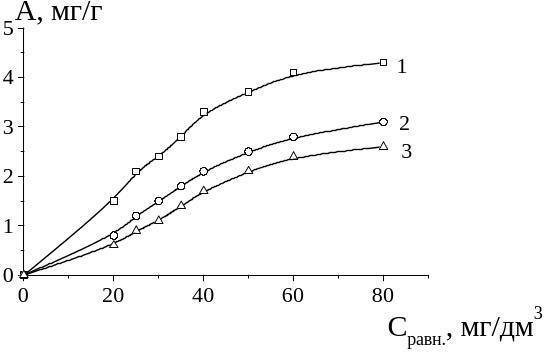
\includegraphics[width=0.8\textwidth]{assets/1033}
	\caption*{}
\end{figure}\begin{figure}[H]
	\centering
	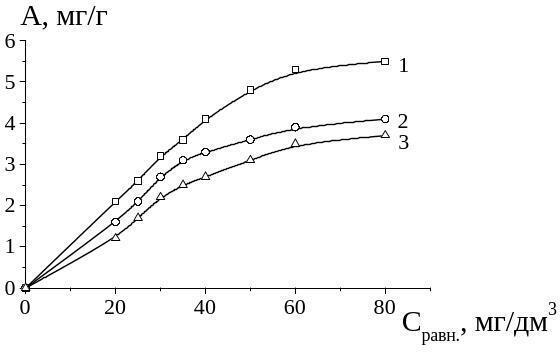
\includegraphics[width=0.8\textwidth]{assets/1034}
	\caption*{}
\end{figure}

А)1 -- рН = 3; 2 -- рН =6; 3 -- рН = 8 Б) 1 -- рН = 3; 2 -- рН =6; 3 --
рН = 8

\textbf{Рис. 1- Зависимость адсорбции БКс на поверхности углистого кека
А и флотационного}

\textbf{концентрата Б, при разных рН среды}

В пользу такого предположения свидетельствуют электрокинетические
данные, которые представлены на рисунке 2. Измерение
электрокинетического потенциала частиц флотируемого материала проводили
в несколько видоизмененном приборе Рабиновича и Фодиман по методу
подвижной границы раздела вода-суспензия {[}11{]}. Показано, что с
увеличением рН среды отрицательный заряд углистого кека увеличивается за
счет преимущественной адсорбции гидроксил-ионов. При увеличении
концентрации БКс отрицательный заряд поверхности также увеличивается. за
счет гидрофобных взаимодействий между углеводородными радикалами БКс и
алифатическими метиленовыми группами циклических нафтеновых фаз
углеродного материала. В результате этого полярные группы БКс будут
обращены в водную фазу, что придает материалу отрицательный
дополнительный заряд. Следует отметить, что из-за большей доступности
гидрофобных участков на поверхности обогащенного углистого кека для
молекул БКс создаются благоприятные условия для сорбции его молекул.

Хорошо известно, что одним из основных факторов, влияющих на адсорбцию
ионов ПАВ на границе раздела фаз, являются взаимодействия в области
двойного электрического слоя. Образование поверхностного заряда при
контакте твердой фазы с водным раствором характерно почти для всех
систем. Только в определенных условиях, существующих в растворе, общий
поверхностный заряд равен нулю, что соответствует точке нулевого заряда
(ТНЗ). Чтобы система в целом оставалась электронейтральной, в растворе
должно находиться одинаковое число ионов с противоположными по знаку
зарядами, эта совокупность электрических зарядов противоположных знаков,
распределенных вдоль границы, раздела двух фаз, образует двойной
электрический слой {[}12,13{]}.

\begin{figure}[H]
	\centering
	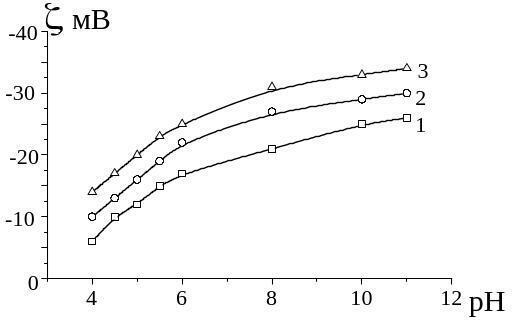
\includegraphics[width=0.8\textwidth]{assets/1035}
	\caption*{}
\end{figure}

\textbf{Рис. 2- Зависимость электрокинетического потенциала частиц
углистого кека (углерод -19,5 \% масс.) (1); флотационного концентрата
(углерод -39,5 \% масс.) (2) и концентрата, после дополнительного
химического обогащения (углерод - 73,2 \%) (3) от рН среды}

Таким образом, проведенные исследования показали, что для работы по
флотационному обогащению углистого кека, учитывая его исходный рН-3, а
так же адсорбционные и электрокинетические характеристики в качестве
реагентов флотации использовались реагенты с преобладанием в основном
терпеновых спиртов.

\emph{2. Определение рабочего индекса измельчаемости углистого кека по
методике Бонда.}

Результаты испытаний по определению индекса измельчаемости углистого
кека приведены в таблице 2.

\textbf{Таблица 2 -- Результаты испытаний по определению индекса
измельчаемости углистого кека}

\begin{longtable}[]{@{}
  >{\raggedright\arraybackslash}p{(\columnwidth - 8\tabcolsep) * \real{0.1924}}
  >{\raggedright\arraybackslash}p{(\columnwidth - 8\tabcolsep) * \real{0.1588}}
  >{\raggedright\arraybackslash}p{(\columnwidth - 8\tabcolsep) * \real{0.2462}}
  >{\raggedright\arraybackslash}p{(\columnwidth - 8\tabcolsep) * \real{0.1623}}
  >{\raggedright\arraybackslash}p{(\columnwidth - 8\tabcolsep) * \real{0.2402}}@{}}
\toprule\noalign{}
\begin{minipage}[b]{\linewidth}\raggedright
Циклы измельчения
\end{minipage} & \begin{minipage}[b]{\linewidth}\raggedright
Число оборотов мельницы за 1 цикл
\end{minipage} & \begin{minipage}[b]{\linewidth}\raggedright
Кол-во материала

-0,074мм, образовавшегося за циклы, г
\end{minipage} & \begin{minipage}[b]{\linewidth}\raggedright
Остаток материала на сите +0,074мм, г
\end{minipage} & \begin{minipage}[b]{\linewidth}\raggedright
Циркуляционная нагрузка,

\%
\end{minipage} \\
\midrule\noalign{}
\endhead
\bottomrule\noalign{}
\endlastfoot
1 & 145 & 230,0 & 770,0 & 335 \\
2 & 325 & 205,0 & 795,0 & 388 \\
3 & 425 & 260,0 & 740,0 & 285 \\
4 & 438 & 275,0 & 725,0 & 264 \\
\end{longtable}

После стабилизации показателей измельчения определялась
гранулометрическая характеристика готового продукта (таблица 3)
{[}14,15{]} методом ситового анализа.

\textbf{Таблица 3 -- Гранулометрическая характеристика исходного и
измельченного кека}

\begin{longtable}[]{@{}
  >{\raggedright\arraybackslash}p{(\columnwidth - 12\tabcolsep) * \real{0.1424}}
  >{\raggedright\arraybackslash}p{(\columnwidth - 12\tabcolsep) * \real{0.1206}}
  >{\raggedright\arraybackslash}p{(\columnwidth - 12\tabcolsep) * \real{0.1524}}
  >{\raggedright\arraybackslash}p{(\columnwidth - 12\tabcolsep) * \real{0.1561}}
  >{\raggedright\arraybackslash}p{(\columnwidth - 12\tabcolsep) * \real{0.1206}}
  >{\raggedright\arraybackslash}p{(\columnwidth - 12\tabcolsep) * \real{0.1525}}
  >{\raggedright\arraybackslash}p{(\columnwidth - 12\tabcolsep) * \real{0.1554}}@{}}
\toprule\noalign{}
\multicolumn{4}{@{}l}{%
\begin{minipage}[b]{\linewidth}\raggedright
Исходный кек
\end{minipage}} & \multicolumn{3}{l@{}}{%
\begin{minipage}[b]{\linewidth}\raggedright
Измельченный кек
\end{minipage}} \\
\midrule\noalign{}
\endhead
\bottomrule\noalign{}
\endlastfoot
\multirow{2}{*}{Размер сита, мм} & \multicolumn{2}{l} & \multirow{2}{*}{суммарный выход
классов, прошедших через сито, \%} & \multicolumn{2}{l} & \multirow{2}{*}{суммарный выход
классов, прошедших через сито, \%} \\
& частный & суммарный & & частный & суммарный \\
-2,5+1,0 & 62,0 & 62,0 & 100 & 10,02 & 10,02 & 100,00 \\
-1,0+0,5 & 13,0 & 75,0 & 38,0 & 5,11 & 15,13 & 89,98 \\
-0,5+0,2 & 11,6 & 86,6 & 25,0 & 25,05 & 40,18 & 84,87 \\
-0,2+0,1 & 7,4 & 94,0 & 13,4 & 10,74 & 50,92 & 59,82 \\
-0,1+0,074 & 4,0 & 98,0 & 6,0 & 21,47 & 72,39 & 49,08 \\
0,074+0,044 & 1,8 & 99,8 & 2,0 & 14,83 & 87,22 & 27,61 \\
Итого: & 100,0 & & & 100,0 & & \\
\end{longtable}

Расход энергии, потребляемой при измельчении, определялся с помощью
трехфазного счетчика. Полезная энергия, затрачиваемая на измельчение,
определялась по разности показаний счетчика при работе мельницы под
нагрузкой и без нее при вращении пустого барабана по формуле:

\begin{figure}[H]
	\centering
	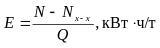
\includegraphics[width=0.8\textwidth]{assets/1036}
	\caption*{}
\end{figure}\textbf{,}

где Е -- удельный расход энергии, затраченной только на измельчение,
кВтч/т;

N -- мощность, потребляемая при измельчении, кВт;

N\textsubscript{х-х} -- мощность холостого хода мельницы без
измельчающей среды, кВт;

Q -- производительность мельницы по исходному питанию, т/ч.

Производительность шаровой мельницы Q рассчитывалась по времени
измельчения t (сек) и навеске кека Р (кг):

\begin{figure}[H]
	\centering
	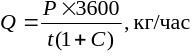
\includegraphics[width=0.8\textwidth]{assets/1037}
	\caption*{}
\end{figure}

где С -- циркулирующая нагрузка, доли единицы, в нашем случае равны
2,68.

\begin{figure}[H]
	\centering
	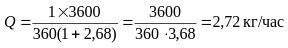
\includegraphics[width=0.8\textwidth]{assets/1038}
	\caption*{}
\end{figure}

Удельный расход энергии равен:

\begin{figure}[H]
	\centering
	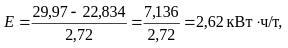
\includegraphics[width=0.8\textwidth]{assets/1039}
	\caption*{}
\end{figure}

Индекс чистой работы измельчения в шаровой мельнице по Бонду определялся
по формуле:

\begin{figure}[H]
	\centering
	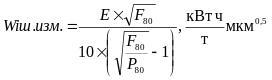
\includegraphics[width=0.8\textwidth]{assets/1040}
	\caption*{}
\end{figure}

F\textsubscript{80} и Р\textsubscript{80} -- размеры отверстий сит,
через которые соответственно проходит 80\% исходного питания и готового
продукта измельчения, мкм.

Параметры F\textsubscript{80} и Р\textsubscript{80} для исследуемого
кека определялся по кривым, представленным на рисунке 3.

\begin{figure}[H]
	\centering
	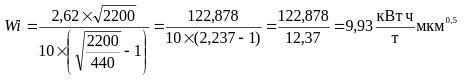
\includegraphics[width=0.8\textwidth]{assets/1041}
	\caption*{}
\end{figure}

\begin{figure}[H]
	\centering
	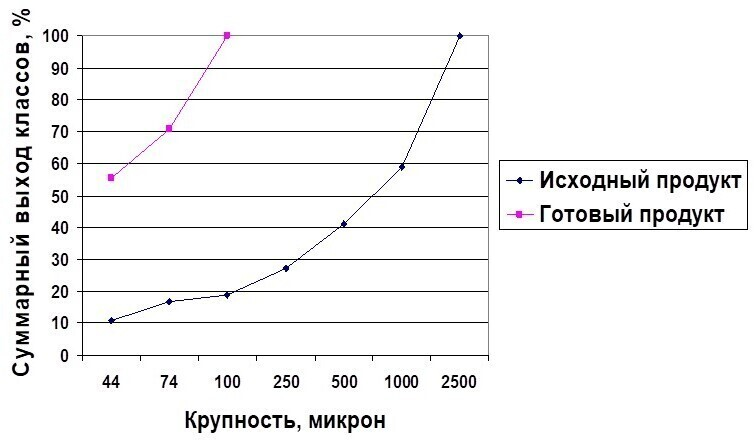
\includegraphics[width=0.8\textwidth]{assets/1042}
	\caption*{}
\end{figure}

\textbf{Рис.3- Гранулометрическая характеристика исходного и конечного
продуктов измельчения}

Анализ полученных расчетных данных и зависимостей позволил сделать вывод
о равномерном распределении работы измельчения без необходимости
проводить многостадийное измельчение для проведения дальнейшего
флотационного обогащения.

Испытание в замкнутом цикле считается установившимся, т.к.
обеспечивается выход готового продукта по массе для 250-270\%
циркулирующей нагрузки.

\emph{3. Обогащение углистого кека пенной флотацией.}

Одним из важных параметров обогащаемого материала является фракционный
состав. Фракционный анализ кека размером зерен менее 0,63 мм проводили
методом центрифугирования. Для исследований использовались растворы
хлористого цинка плотностью от 1300 кг/м\textsuperscript{3} до 1800
кг/м\textsuperscript{3} . Результаты фракционного и ситового анализа
представлены в таблице 4 и 5.

\textbf{Таблица 4 - Фракционный анализ углистого кека}

\begin{longtable}[]{@{}
  >{\raggedright\arraybackslash}p{(\columnwidth - 6\tabcolsep) * \real{0.2729}}
  >{\raggedright\arraybackslash}p{(\columnwidth - 6\tabcolsep) * \real{0.1513}}
  >{\raggedright\arraybackslash}p{(\columnwidth - 6\tabcolsep) * \real{0.2731}}
  >{\raggedright\arraybackslash}p{(\columnwidth - 6\tabcolsep) * \real{0.3027}}@{}}
\toprule\noalign{}
\endhead
\bottomrule\noalign{}
\endlastfoot
\multirow{2}{*}{Плотность фракций, кг/м\textsuperscript{3}} &
\multirow{2}{*}{Выход фракций,

\%} &
\multicolumn{2}{>{\raggedright\arraybackslash}p{(\columnwidth - 6\tabcolsep) * \real{0.5758} + 2\tabcolsep}@{}} \\
& & всплывшие фракции & невсплывшие фракции \\
\textless{} 1300

1300-1400

1400-1500

1500-1800

\textgreater{} 1800 & 60,5

22,6

4,9

3,1

8,9 & 60,5

83,1

88,0

91,1

100 & 100

39,5

16,9

12,0

8,9 \\
\end{longtable}

Параллельно с фракционным анализом был проведен ситовый анализ
используемого кека для флотации. Класс крупности рабочей фракции
составил − 0,63 мм.

\textbf{Таблица 5 - Ситовой состав исходной пробы углистого кека}

\begin{longtable}[]{@{}
  >{\raggedright\arraybackslash}p{(\columnwidth - 8\tabcolsep) * \real{0.2899}}
  >{\raggedright\arraybackslash}p{(\columnwidth - 8\tabcolsep) * \real{0.1629}}
  >{\raggedright\arraybackslash}p{(\columnwidth - 8\tabcolsep) * \real{0.1776}}
  >{\raggedright\arraybackslash}p{(\columnwidth - 8\tabcolsep) * \real{0.1925}}
  >{\raggedright\arraybackslash}p{(\columnwidth - 8\tabcolsep) * \real{0.1771}}@{}}
\toprule\noalign{}
\endhead
\bottomrule\noalign{}
\endlastfoot
Фракция, мм & -0,63+0,20 & -0,20+0,074 & -0,074+0,044 & -0,044+0,00 \\
Содержание, \% масс. & 11,3 & 23,7 & 46,1 & 18,9 \\
\end{longtable}

При флотационном обогащении углистого кека средняя плотность пульпы
принималась как р=2,8÷3,3 или Т:Ж = 300÷350 г/л. Такое соотношение Т:Ж
было определено как оптимальное. Учитывая адсорбционные и
электрокинетические характеристики исследуемого материала, описанных
выше, в качестве реагентов для пенной флотации были опробованы
синтетические ацетат 3-амилтетрагидропиран-4-ол и ксантогенат
1-метил-3-карбэтокси-1,2,5,6-тетрагидропиридин-4-ол, синтезированные в
НАО «КазНУ им. аль-Фараби», а также коммерческий реагент-собиратель
Flotol B. В качестве собирателя керосин осветленный. Дозирование
флотационных реагентов велось дробно, через дозаторы. Режимные параметры
ведения процесса флотации экспериментально определенные, как
оптимальные, представлены в таблице 6.

\textbf{Таблица 6 -- Режимные параметры технологического процесса
флотации, пересчитанные на 1 тонну углистого кека на флотацию}

\begin{longtable}[]{@{}
  >{\raggedright\arraybackslash}p{(\columnwidth - 4\tabcolsep) * \real{0.6434}}
  >{\raggedright\arraybackslash}p{(\columnwidth - 4\tabcolsep) * \real{0.1753}}
  >{\raggedright\arraybackslash}p{(\columnwidth - 4\tabcolsep) * \real{0.1814}}@{}}
\toprule\noalign{}
\endhead
\bottomrule\noalign{}
\endlastfoot
Наименование параметра & Ед. изм. & Значение \\
Расход вспенивателя на 1 тонну руды & г & 320 \\
Расход собирателя на 1 тонну руды & г & 280 \\
Содержание класса -0,074 мм в питании флотации & \% & 65 \\
Плотность питания основной флотации & \% тв & 30 \\
\end{longtable}

Основной характеристикой качества флотореагентов является устойчивость
пены. Результаты проведенных нами исследований этого показателя для
применяемых флотореагентов представлены в таблице 7 {[}16,17{]}.

Таблица 7 -- Время устойчивости пены при различных флотореагентах

\begin{longtable}[]{@{}
  >{\raggedright\arraybackslash}p{(\columnwidth - 6\tabcolsep) * \real{0.3442}}
  >{\raggedright\arraybackslash}p{(\columnwidth - 6\tabcolsep) * \real{0.2303}}
  >{\raggedright\arraybackslash}p{(\columnwidth - 6\tabcolsep) * \real{0.2103}}
  >{\raggedright\arraybackslash}p{(\columnwidth - 6\tabcolsep) * \real{0.2151}}@{}}
\toprule\noalign{}
\multirow{2}{*}{\begin{minipage}[b]{\linewidth}\raggedright
Тип флотореагента
\end{minipage}} & \multicolumn{3}{l@{}}{%
\begin{minipage}[b]{\linewidth}\raggedright
Время устойчивости, мин.
\end{minipage}} \\
& \begin{minipage}[b]{\linewidth}\raggedright
начальный сбор
\end{minipage} & \begin{minipage}[b]{\linewidth}\raggedright
средний сбор
\end{minipage} & \begin{minipage}[b]{\linewidth}\raggedright
конечный сбор
\end{minipage} \\
\midrule\noalign{}
\endhead
\bottomrule\noalign{}
\endlastfoot
Flotol B & \textgreater60 & 10-15 & \textless1 \\
Ацетат 3-амилтетра-гидропиран-4-ола & 5-10 & \textless1 & \textless1 \\
1-метил-3-карбэтокси-1,2,5,6-тетра-гидропиридин-4-ола & 10-15 & 1-2 &
\textless1 \\
\end{longtable}

По проведенным исследованиям, наиболее эффективным пенообразователем
зарекомендовал Flotol В. Он и был определен, как наиболее перспективный.
Дальнейшие работы по флотации углистого кека, в качестве вспенивается
проводили с этим реагентом. Flotol В состоит в основном из терпеновых
спиртов, в которых терпинеол является основным компонентом.
Характеристики процесса флотации исследуемых флотореагентов показаны в
таблицах 8-9.

\textbf{Таблица 8 \emph{-} Показатели обогащения углистого кека, \%}

\begin{longtable}[]{@{}
  >{\raggedright\arraybackslash}p{(\columnwidth - 6\tabcolsep) * \real{0.4939}}
  >{\raggedright\arraybackslash}p{(\columnwidth - 6\tabcolsep) * \real{0.1687}}
  >{\raggedright\arraybackslash}p{(\columnwidth - 6\tabcolsep) * \real{0.1381}}
  >{\raggedright\arraybackslash}p{(\columnwidth - 6\tabcolsep) * \real{0.1994}}@{}}
\toprule\noalign{}
\multirow{2}{*}{\begin{minipage}[b]{\linewidth}\raggedright
Показатель
\end{minipage}} & \multicolumn{3}{l@{}}{%
\begin{minipage}[b]{\linewidth}\raggedright
Флотореагент
\end{minipage}} \\
& \begin{minipage}[b]{\linewidth}\raggedright
Flotol B
\end{minipage} & \begin{minipage}[b]{\linewidth}\raggedright
Ацетат
\end{minipage} & \begin{minipage}[b]{\linewidth}\raggedright
Ксантогенат
\end{minipage} \\
\midrule\noalign{}
\endhead
\bottomrule\noalign{}
\endlastfoot
Содержание углерода в кеке & 19,5 & 19,5 & 19,5 \\
Выход концентрата & 35 & 22 & 31 \\
Содержание углерода в концентрате & 39,5 & 35,2 & 29,4 \\
Содержание углерода в хвостах & 8,1 & 12,5 & 15,5 \\
Извлечение углерода в концентрат & 73,4 & 40,5 & 47,5 \\
\end{longtable}

Из результатов таблицы 8 видно, что оптимальным соотношением
флотационных реагентов, является совместное использование, в качестве
собирателя -- керосина и пенообразователя -- реагент «Flotol B», при
этом в процессе флотационного обогащения, в одну стадию без
дополнительной перечистки, содержание углерода в концентрате увеличилось
до 40,0 ± 2 \%.

\textbf{Таблица 9 \emph{--} Результаты флотационного обогащения
углистого кека}

\begin{longtable}[]{@{}
  >{\raggedright\arraybackslash}p{(\columnwidth - 16\tabcolsep) * \real{0.0443}}
  >{\raggedright\arraybackslash}p{(\columnwidth - 16\tabcolsep) * \real{0.1045}}
  >{\raggedright\arraybackslash}p{(\columnwidth - 16\tabcolsep) * \real{0.0895}}
  >{\raggedright\arraybackslash}p{(\columnwidth - 16\tabcolsep) * \real{0.1195}}
  >{\raggedright\arraybackslash}p{(\columnwidth - 16\tabcolsep) * \real{0.1046}}
  >{\raggedright\arraybackslash}p{(\columnwidth - 16\tabcolsep) * \real{0.1493}}
  >{\raggedright\arraybackslash}p{(\columnwidth - 16\tabcolsep) * \real{0.1045}}
  >{\raggedright\arraybackslash}p{(\columnwidth - 16\tabcolsep) * \real{0.1344}}
  >{\raggedright\arraybackslash}p{(\columnwidth - 16\tabcolsep) * \real{0.1494}}@{}}
\toprule\noalign{}
\endhead
\bottomrule\noalign{}
\endlastfoot
\multirow{3}{*}{№

п/п} &
\multicolumn{4}{>{\raggedright\arraybackslash}p{(\columnwidth - 16\tabcolsep) * \real{0.4181} + 6\tabcolsep}} &
\multirow{3}{*}{Сод-е

углерода,

\% мас.} & \multirow{3}{*}{Извлечение

углерода,

\%} \\
& Собира-тель &
\multicolumn{3}{>{\raggedright\arraybackslash}p{(\columnwidth - 16\tabcolsep) * \real{0.3136} + 4\tabcolsep}}{%
пенообразователь} \\
& керосин & Flotol B & Ксанто-генат & Ацетат \\
\multirow{2}{*}{1} & \multirow{2}{*}{2,0} & \multirow{2}{*}{1,8} &
\multirow{2}{*}{-} & \multirow{2}{*}{-} & концентрат & 35,2 & 39,5 &
73,4 \\
& & & & & хвосты & 64,8 & 8,1 & - \\
\multirow{2}{*}{3} & \multirow{2}{*}{2,0} & \multirow{2}{*}{-} &
\multirow{2}{*}{-} & \multirow{2}{*}{5} & концентрат & 22,0 & 35,2 &
40,5 \\
& & & & & хвосты & 78,0 & 12,5 & - \\
\multirow{2}{*}{4} & \multirow{2}{*}{2,0} & \multirow{2}{*}{1,8} &
\multirow{2}{*}{5} & \multirow{2}{*}{-} & концентрат & 36,2 & 32,2 &
61,3 \\
& & & & & хвосты & 63,8 & 9,6 & - \\
\end{longtable}

Таким образом, изучен процесс флотационного извлечения углерода из
некондиционного углистого кека после обогащения ванадиевой руды.
Получены углеродные концентраты, стабильные по химическому составу.
Химический состав исходного кека и продуктов обогащения представлены в
таблице 1. Учитывая гибкую схему ведения процесса обогащения возможно
варьировать содержание углерода и минеральной составляющей в
концентратах, что является важным экономическим и технологическим
фактором при расчете химико-технологических процессов. Полученные
углеродные концентраты могут быть использованы в технологических
процессах производства сорбентов, композиционных материалов и
эластомеров, в качестве альтернативных товарных материалов на основе
аморфного углерода.

\textbf{Выводы.} Изучен химический анализ углистого кека (отход после
автоклавного выщелачивания ванадиевой руды), в основу состава которого
входит углерод, диоксид кремния, соединения щелочных и щелочноземельных
металлов, а также соединения железа и алюминия. Для возможности
раскрытия углистого кека для флотационного обогащения и дальнейшего
внедрения в производственный процесс проведены исследования и расчеты
определения рабочего индекса измельчаемости по методике Бонда в шаровой
мельнице. Анализ полученных расчетных данных и зависимостей позволил
сделать вывод о равномерном распределении работы измельчения без
необходимости проводить многостадийное измельчение для проведения
дальнейшего флотационного обогащения. Испытание в замкнутом цикле
считается установившимся, т.к. обеспечивается выход готового продукта по
массе для 250-270\% циркулирующей нагрузки. Определена средняя плотность
пульпы р=2,8÷3,3. В качестве реагентов для пенной флотации опробованы
синтетические ацетат 3-амилтетрагидропиран-4-ол и ксантогенат
1-метил-3-карбэтокси-1,2,5,6-тетрагидропиридин-4-ол и коммерческий
реагент-собиратель Flotol B. В качестве вспенивателя керосин
осветленный. В процессе обогащения в одну стадию без дополнительной
перечистки содержание углерода в концентрате увеличилось до 40,0 ± 2 \%.
Полученные углеродные концентраты стабильны по химическому составу и
могут быть использованы в технологических процессах производств в
качестве альтернативных товарных материалов на основе аморфного
углерода.

\emph{\textbf{Финансирование.}} Работа выполнена в рамках исследования,
профинансированного Комитетом науки Министерства науки и высшего
образования Республики Казахстан (Грант № BR21882289).

\textbf{Литература}

1.Ахременко Н.П. Мониторинг обращения с вторичными материальными
ресурсами на территории региона, на примере Ленинградской области.
Выпускная квалификационная работа, уровень образования: Магистратура,
направление 05.04.06 «Экология и природопользование». -
Санкт-Петербургский государственный университет. - Санкт-Петербург,
2019. - 80 с.

2.ГОСТ Р 54098-2010. Ресурсосбережение. Вторичные материальные ресурсы.
Термины и определения. -- М.: Стандартинформ, 2011. - 19 с.

3. Материал из Википедии --- свободной энциклопедии
\textbf{«}Каратауский ванадиевый бассейн».
https://ru.wikipedia.org/wiki/\%D0\%9A\%D0\%B0\%D1\%80\%D0\%B0\%D1\%82\%D0\%B0\%D1\%83\%D1\%81\%D0\%BA\%D0\%B8\%D0\%B9\_\%D0\%B2\%D0\%B0\%D0\%BD\%D0\%B0\%D0\%B4\%D0\%B8\%D0\%B5\%D0\%B2\%D1\%8B\%D0\%B9\_\%D0\%B1\%D0\%B0\%D1\%81\%D1\%81\%D0\%B5\%D0\%B9\%D0\%BD

4. Вохидов Б.Р., Мамараимов Г.Ф., Хасанов А.С. Разработка технологии
получения пятиокиси ванадия из минерального и техногенного сырья //
Universum: технические науки: электрон. научн. журн., 2020.- № 3 (72).
https://7universum.com/ru/tech/archive/item/9085

5. ГОСТ 4790---93. ТОПЛИВО ТВЕРДОЕ. Определение и представление
показателей фракционного анализа. Общие требования к аппаратуре и
методике. -- ИПК Издательство стандартов, 2002. - 19 с.

6. Фридман С.Э., Щербаков O.K., Еремин Н.Я. Основы обогащения руд и
углей и окускование концентратов. - М.: Недра. 1991.- 270 с.

7. Бедрань, Н.Г. Флотационные машины для обогащения угля. -- М.: Недра,
1968. - 127 с.

8. Богданов О. С., Максимов И. И., Поднек А. К., Янис Н. А. Теория и
технология флотации руд. - М.: Недра, 1990. - 363 с.

9. Ефремов С.А. Технология производства углерод-минеральных материалов
на основе шунгитовых пород: дис. \ldots{} д.х.н. -- Алматы, 2010. -- 307
с.

10. Е.Р. Сабырбаев, К.Б. Мусабеков, Н.К. Тусупбаев. Поверхностные и
флотационные свойства модифицирующей добавки бутилтриэтилентетрамина //
Вестник КазНУ. Серия химическая, 2014.- №1 (73).- С. 40-48.

11. Духин С.С. Электропроводность и электрокинетические свойства
дисперсных систем. -- Киев: Наукова думка, 1975.-- 246 с.

12. R. Sato Elektron diffraction investigation of xanthates on cooper
activated spalerite cleavage face // Journal Mining Institute
Japan,1971.- Vol.70. - Р. 28-33.

13. Нечипуренко С.В., Калугин С.Н., Ефремов С.А., Асылханов Ж.С.,
Балтабаев А., Кушекова А.К. Исследование флотирующей способности
производных тетрагидропирана и пиперидина в процессах обогащения
шунгитовых пород// Хим. журн. Казахстана. - 2006. - № 4(13). - С.
221-224.

14. Л.С. Читалов, В.В. Львов. Сравнительная оценка методов определения
рабочего индекса шарового измельчения бонда // ГИАБ. Горный
информационно-аналитический бюллетень. -2021.- N.1.- С.130-145. DOI:
10.25018/0236-1493-2021-1-0-130-145

15. Читалов Л.С. Разработка комплексного метода оценки эффективности
процессов измельчения сульфидных медно-никелевых руд: дис. \ldots{}
к.т.н. - Санкт-Петербург, 2021. -- 118 с.

16. Обогащение угля. Справочник / под. Ред. Благова И.С., Коткина А.М.,
Зарубина Л.С., 2-е изд. - М.: Недра, 1984. - 614 с.

17. Хан Г.А., Габриелова Л.И., Власова Н.С. Флотационные реагенты и их
применение. - М.: Недра, 1986. - 270 с.

\textbf{References}

1.Ahremenko N.P. Monitoring obrashhenija s vtorichnymi
material\textquotesingle nymi resursami na territorii regiona, na
primere Leningradskoj oblasti. Vypusknaja kvalifikacionnaja rabota,
uroven\textquotesingle{} obrazovanija: Magistratura, napravlenie
05.04.06 «Jekologija i prirodopol\textquotesingle zovanie». -
Sankt-Peterburgskij gosudarstvennyj universitet. - Sankt-Peterburg,
2019. - 80 s.{[}Russian{]}

2.GOST R 54098-2010. Resursosberezhenie. Vtorichnye
material\textquotesingle nye resursy. Terminy i opredelenija. -- M.:
Standartinform, 2011. - 19 s. .{[}Russian{]}

3. Material iz Vikipedii --- svobodnoj jenciklopedii «Karatauskij
vanadievyj.{[}Russian{]}

https://ru.wikipedia.org/wiki/\%D0\%9A\%D0\%B0\%D1\%80\%D0\%B0\%D1\%82\%D0\%B0\%D1\%83\%D1\%81\%D0\%BA\%D0\%B8\%D0\%B9\_\%D0\%B2\%D0\%B0\%D0\%BD\%D0\%B0\%D0\%B4\%D0\%B8\%D0\%B5\%D0\%B2\%D1\%8B\%D0\%B9\_\%D0\%B1\%D0\%B0\%D1\%81\%D1\%81\%D0\%B5\%D0\%B9\%D0\%BD

4. Vohidov B.R., Mamaraimov G.F., Hasanov A.S. Razrabotka tehnologii
poluchenija pjatiokisi vanadija iz mineral\textquotesingle nogo i
tehnogennogo syr\textquotesingle ja // Universum: tehnicheskie nauki:
jelektron. nauchn. zhurn., 2020.- № 3 (72).
https://7universum.com/ru/tech/archive/item/9085.{[}Russian{]}

5. GOST 4790---93. TOPLIVO TVERDOE. Opredelenie i predstavlenie
pokazatelej frakcionnogo analiza. Obshhie trebovanija k apparature i
metodike. -- IPK Izdatel\textquotesingle stvo standartov, 2002. - 19 s.
.{[}Russian{]}

6. Fridman S.Je., Shherbakov O.K., Eremin N.Ja. Osnovy obogashhenija rud
i uglej i okuskovanie koncentratov. - M.: Nedra. 1991.- 270 s.
.{[}Russian{]}

7. Bedran\textquotesingle, N.G. Flotacionnye mashiny dlja obogashhenija
uglja. -- M.: Nedra, 1968. - 127 s. .{[}Russian{]}

8. Bogdanov O. S., Maksimov I. I., Podnek A. K., Janis N. A. Teorija i
tehnologija flotacii rud. - M.: Nedra, 1990. - 363 s. .{[}Russian{]}

9. Efremov S.A. Tehnologija proizvodstva
uglerod-mineral\textquotesingle nyh materialov na osnove shungitovyh
porod: dis. \ldots{} d.h.n.-Almaty, 2010.-307 s.{[}Russian{]}

10. E.R. Sabyrbaev, K.B. Musabekov, N.K. Tusupbaev. Poverhnostnye i
flotacionnye svojstva modificirujushhej dobavki butiltrijetilentetramina
// Vestnik KazNU. Serija himicheskaja, 2014.- №1 (73).- S. 40-48.
{[}Russian{]}

11. Duhin S.S. Jelektroprovodnost\textquotesingle{} i
jelektrokineticheskie svojstva dispersnyh sistem. -- Kiev: Naukova
dumka, 1975. 246 s. {[}Russian{]}

12. R. Sato Elektron diffraction investigation of xanthates on cooper
activated spalerite cleavage face // Journal Mining Institute
Japan,1971.- Vol.70. - R. 28-33. {[}Russian{]}

13. Nechipurenko S.V., Kalugin S.N., Efremov S.A., Asylhanov Zh.S.,
Baltabaev A., Kushekova A.K. Issledovanie flotirujushhej sposobnosti
proizvodnyh tetragidropirana i piperidina v processah obogashhenija
shungitovyh porod// Him. zhurn. Kazahstana. - 2006. - № 4(13). - S.
221-224. {[}Russian{]}

14. L.S. Chitalov, V.V. L\textquotesingle vov.
Sravnitel\textquotesingle naja ocenka metodov opredelenija rabochego
indeksa sharovogo izmel\textquotesingle chenija bonda // GIAB. Gornyj
informacionno-analiticheskij bjulleten\textquotesingle. -2021.- N.1.-
S.130-145. DOI: 10.25018/0236-1493-2021-1-0-130-145.{[}Russian{]}

15. Chitalov L.S. Razrabotka kompleksnogo metoda ocenki jeffektivnosti
processov izmel\textquotesingle chenija sul\textquotesingle fidnyh
medno-nikelevyh rud: dis. \ldots{} k.t.n. - Sankt-Peterburg, 2021.-118
s. .{[}Russian{]}

16. Obogashhenie uglja. Spravochnik / pod. Red. Blagova I.S., Kotkina
A.M., Zarubina L.S., 2-e izd. - M.: Nedra, 1984. - 614 s. {[}Russian{]}

17. Han G.A., Gabrielova L.I., Vlasova N.S. Flotacionnye reagenty i ih
primenenie. - M.: Nedra, 1986. - 270 s. {[}Russian{]}

\emph{\textbf{Сведения об авторах}}

НечипуренкоС.В.- к.т.н., доцент, Казахский Национальный университет
имени аль-Фараби», Алматы, Казахстан, e-mail: nechipurenkos@mail.ru;

Канаев Р.К.- магистрант Казахский национальный университет имени
аль-Фараби», Алматы, Казахстан, e-mail: ramazankanaev@gmail.com;

Ефремов С.А. - д.х.н., профессор, Казахский национальный университет
имени аль-Фараби», Алматы, Казахстан, e-mail: nechipurenkos@mail.ru;

Кузнецов А.А.- коммерческий директор ТОО «Фирма Балауса», Алматы,
Казахстан, e-mail:~akuz@ferro-alloy.com;

Мун Г.А. -д.х.н., профессор,природных соединений и полимеров, Казахский
национальный университет имени аль-Фараби», Алматы, Казахстан, e-mail:
mungrig@yandex.ru

\emph{\textbf{Information about authors}}

Nechipurenko~S.V. - c.t.sc, Associate Professor al-Farabi Kazakh
National University, Almaty, Kazakhstan, e-mail:~nechipurenkos@mail.ru;

Kanaev~R.K.-Master student, al-Farabi Kazakh National University,
Almaty, Kazakhstan,~e-mail:~ramazankanaev@gmail.com;

Yefremov S.A.-~Doctor of Chemical Sciences, Professor,al-Farabi Kazakh
National University, Almaty, Kazakhstan, e-mail:~nechipurenkos@mail.ru;

KuznetsovA.A.-Commercial Director of Balausa Firm LLP, Almaty,
Kazakhstan, e-mail:~akuz@ferro-alloy.com;

Mun~G.A.-Doctor of Chemical Sciences, Professor, al-Farabi Kazakh
National University, Almaty, Kazakhstan, e-mail:~mungrig@yandex.ru

ҒТАМР 31.15.37

\textbf{БЕНТОНИТ САЗЫН ТАУ-КЕН ӨНДІРІСІНІҢ ШАХТА СУЛАРЫН ТАЗАРТУДАҒЫ
ҚОЛДАНУ ТИІМДІЛІГІ}

\textbf{\textsuperscript{1,3} О.В. Рожкова,\textsuperscript{2} Ш.А.
Мұздыбаева, \textsuperscript{3}А.Б. Бөкеева, \textsuperscript{3}С.Ж.
Құдайбергенова,}

\textbf{\textsuperscript{3,4} В.И. Рожков, \textsuperscript{1}М.Т.
Ермеков, \textsuperscript{5} Ж.Т.Нұртай}

\textsuperscript{1} «Science and Technology Solutions» АҚ, Алматы,
Қазақстан,

\textsuperscript{2}Халықаралық инженерлік-технологиялық университеті,
Алматы, Қазақстан,

\textsuperscript{3} КЕАҚ «С.Сейфуллин атындағы Қазақ агротехникалық
зерттеу университеті»,

Астана, Қазақстан,

\textsuperscript{4}«Алтай геологиялық-экологиялық институты» ЖШС,
Өскемен, Қазақстан,

\textsuperscript{5} «Қ.Құлажанов атындағы Қазақ технология және бизнес
университеті» АҚ, Астана, Қазақстан,

Корреспондент-автор: rozhkova.o@stsolutions.kz

Металлургиялық кәсіпорындардың ағынды суларын тазарту мақсатында
Шығыс-Қазақстан облысы Таған кен орнының бентониті зерттелген. Табиғи
сорбенттің және оның белсендірілген түрлерінің физика-химиялық
сипаттамаларын зерттеу үшін заманауи зерттеу әдістері қолданылған:
атомды-абсорбциялық спектрометрия, индуктивті байланысқан плазмамен
масс-спектрометрия, полярография және рентгенфлуоресцентті
спектрометрия, энергодисперсиондық талдау қосымшасымен электрондық
микроскопия. Бентониттің термиялық және термоқышқылдық белсендендірілуі
қарастырылған. Белсендендірілген формалардың құрылымы электрондық
микроскоп көмегімен анықталған. Табиғи және белсендендірілген түрлерінің
микроқұрылымдарын электрондық микроскоппен салыстыру кезінде құрылымының
ең көп өзгеруі термоқышқылдық белсендендіру кезінде жүргізілетінін
көрсетеді. Бентониттің кеуектілігі артып, беткі қабаты көбірек босайды.

Полиметалдық кен орнының ағынды суларын тазатру үшін бентониттің табиғи
және белсендендірілген түрлері қолданылған. Осы кезде
Cu\textsuperscript{2+}, Pb\textsuperscript{2+}, Cd\textsuperscript{2+},
Zn\textsuperscript{2+} иондарының ең көп сіңірілуі (94-99,6\%) шекті
рұқсат етілген концентрацияларға дейін термоқышқылды белсендендірілген
бентонитті қолданғанда іске асатыны байқалған. Бұл зерттеу Таған кен
орнының термоқышқылды белсендіріліген бентонитін металлургиялық
кәсіпорындардың ағынды суларын ауыр металдардан тазартуда қолдануда
тиімді екенін көрсетеді.

\textbf{Түйін сөздер:} бентонит сазы, ағынды сулар, қышқылдық
белсендіру, термоқышқылдық белсендіру.

\textbf{ЭФФЕКТИВНОСТЬ ИСПОЛЬЗОВАНИЯ БЕНТОНИТОВОЙ ГЛИНЫ В ОЧИСТКЕ ШАХТНОЙ
ВОДЫ ГОРНО-РУДНОЙ ПРОМЫШЛЕННОСТИ}

\textbf{\textsuperscript{1,3}О.В.Рожкова,
\textsuperscript{2}Ш.А.Муздыбаева, \textsuperscript{3}А.Б.Букеева,}

\textbf{\textsuperscript{3}С.Ж. Кудайбергенова,
\textsuperscript{3,4}В.И.Рожков, \textsuperscript{1}М.Т.
Ермеков\textsubscript{,} \textsuperscript{5} Ж.Т.Нуртай}

\textsuperscript{1} АО «Science and Technology Solutions», Алматы,
Казахстан,

\textsuperscript{2}Международный инженерно-технологический университет,
Алматы, Казахстан

\textsuperscript{3}НАО \textsuperscript{«}Казахский~агротехнический
исследовательский университет им.~С.~Сейфуллина»,

Астана, Казахстан,

\textsuperscript{4}ТОО «Алтайский геолого-экологический институт»,
Усть-Каменогорск, Казахстан,

\textsuperscript{5}АО «Казахский Университет технологии и бизнеса им
К.Кулажанова», Астана, Казахстан,

e-mail: rozhkova.o@stsolutions.kz

Изучен бентонит Таганского месторождения Восточно-Казахстанской области
с целью применения для очистки сточных вод металлургических предприятий.
Для изучения физико-химических характеристик сорбентов активированных
частиц были привлечены современные методы исследования:
атомно-абсорбционная спектрометрия, масс-спектрометрия с
индуктивно-связанной плазмой, полярография и рентгенофлуо-ресцентная
спектроскопия, электронная микроскопия.

Рассмотрена термическая и термокислотная активация бентонита. Структуру
активированных форм определяли с помощью электронного микроскопа. При
сравнении микроструктур природного и активированного типов с помощью
электронного микроскопа показано, что максимальное изменение структуры
происходит при термокислотной активации. Пористость бентонита
увеличивается, поверхностный слой становится более рыхлым. Природные и
активированные формы бентонита использовались для очистки сточных вод от
полиметаллических отложений. В это время было замечено, что максимальное
поглощение ионов Cu\textsuperscript{2+}, Pb\textsuperscript{2+},
Cd\textsuperscript{2+}, Zn\textsuperscript{2+} (94-99,6\%) реализуется
при использовании термокислотно-активированного бентонита до предельно
допустимых концентраций. Проведенное исследование показывает, что
термокислотно-активированный бентонит Таганского месторождения
эффективен при очистке сточных вод от тяжелых металлов на
металлургических предприятиях.

\textbf{Ключевые слова:} бентонитовая глина, сточные воды, кислотная
активация, термокислотная активация.

\textbf{EFFECTIVENESS OF USING BENTONITE CLAY IN THE PURIFICATION OF
MINE WATER IN THE MINING INDUSTRY}

\textbf{\textsuperscript{1,3}O.V. Rozhkova,
\textsuperscript{2}Ш.А.Муздыбаева, \textsuperscript{3}A.B.Bukeeva,
\textsuperscript{3}S.Zh.Kudaibergenova,}

\textbf{\textsuperscript{3,4}V.I. Rozhkov, \textsuperscript{1}M.T.,
Yermekov,\textsuperscript{5}Zh.T.Nurtai}

\textsuperscript{1} SC «Science and Technology Solutions», Almaty,
Kazakhstan,

\textsuperscript{2} NC JSC «Al-Farabi Kazakh National University»,

Almaty, Kazakhstan,

\textsuperscript{3} NAO «S. Seifullin Kazakh Agrotechnical Research
University», Astana, Kazakhstan,

\textsuperscript{4}Altai Geological and Ecological Institute LLP,
Ust-Kamenogorsk, Kazakhstan,

\textsuperscript{5} JSC «Kazakh University of Technology and Business
named after K. Kulazhanov», Astana, Kazakhstan,

e-mail: rozhkova.o@stsolutions.kz

Bentonite from the Taganskoe deposit in the East Kazakhstan region has
been studied for the purpose of using it for wastewater treatment of
metallurgical enterprises. To study the physicochemical characteristics
of activated particle sorbents, modern research methods were used:
atomic absorption spectrometry, inductively coupled plasma mass
spectrometry, polarography and X-ray fluorescence spectroscopy, electron
microscopy.

Thermal and thermoacid activation of bentonite is considered. The
structure of the activated forms was determined using an electron
microscope. When comparing microstructures of natural and activated
types using an electron microscope, it was shown that the maximum change
in structure occurs during thermal acid activation. Natural and
activated forms of bentonite have been used to purify wastewater from
polymetallic deposits. At this time, it was noticed that the maximum
absorption of Cu\textsuperscript{2+}, Pb\textsuperscript{2+},
Cd\textsuperscript{2+}, Zn\textsuperscript{2+} ions (94-99.6\%) is
realized when using thermal acid-activated bentonite up to the maximum
permissible concentrations. The study shows that thermal acid-activated
bentonite from the Taganskoye deposit is effective in treating
wastewater from heavy metals at metallurgical enterprises.

\textbf{Keywords:} bentonite clay, wastewater, acid activation, thermal
acid activation.

\textbf{Кіріспе.} Металлургиялық кәсіпорындар қоршаған ортаны ірі
ластаушылардың бірі болып табылады, соның ішінде ағынды сулармен.
Құрамында жүзгіндер, кен бөлшектері, ауыр металдардың катиондары болатын
металлургиялық кәсіпорындардың ағынды суларын бірнеше сатыда тазартады.
Өнеркәсіптік ағынды суларды тазартуда ең озық әдістердің бірі сорбциялық
әдістер болып табылады. Бұлардың артықшылығы тиімділігімен төменгі
бағасында. Соның ішінде бентониттер, цеолиттер сияқты табиғи сорбенттер
қызығушылық тудырады.

Қазақстанда бентонит сазы өндіріліп, қайта өңделетін ірі Таған кен орны
бар (Ақжар ауылы, Шығыс-Қазақстан облысы). Мамандардың пайымдауынша бұл
кеннің қоры шамамен 9 млн. тоннадан көп. Таған кен орнының қорлары батыс
қапталда (32\% салыстырмалы) және шығыс қапталда сілтілі жер сорттары
(60\%) берілген. Таған бентониттерінің жоғары технологиялық өнімділігі
монтмориллониттің кристалдық құрылымының ерекшеліктеріне, материал
құрамына, дисперстілігіне байланысты және сорбенттер өндірісіне
қойылатын шикізатқа қойылатын талаптарға сәйкес {[}1{]}.

Бентониттер қатпарлы саз типті силикаттар класына жатады. Олар жақсы
адсорбциялық қасиет көрсететін арзан материалдарға жатады. Саздың
меншікті бетінің ауданын ұлғайту үшін қышқылдық, термиялық, тұздық және
басқа белсендірулерді жүргізуге болады.

Бентониттің сорбциялық, ионалмасу қасиеттері ағынды суларды мұнай
өнімдерінен, органикалық заттардың эмульсияларымен дисперсияларынан,
ауыр металдардан тазартуда қолданылады {[}2{]}. Бірақ бентонит сазы,
суды қоспалардан тазарта отырып, оның лайлығын арттырады. Бұл мәселені
бентониттің түрлі полимерлермен композицияларын қолдана отырып шешуге
болады.

Бентонит құрылымының түрлі функционалдық топтармен, физикалық әсерлермен
(ультрадыбыс, температура) модификациялануын зерттеу оның адсорбциялық
қабілетін арттыруға болатынын көрсетеді. Табиғи сорбенттер мен олардың
белсендірілген түрлерін ағынды суларды тазарту үшін пайдалану бойынша
зерттеулер, сандық көрсеткіштерге көбірек көңіл бөле отырып, айтарлықтай
қарқынды жүргізілуде. Сонымен бірге активтену кезінде сорбент
құрылымының өзгеруі, ерітіндідегі және дисперстік фаза бетіндегі
макроиондардың параметрлері арасындағы байланыс, полиэлектролиттердің
және олардың комплекстерінің адсорбциялық қабаттарының құрылымы,
процестің кинетикасы, металл иондарының гидродисперсия бөлшектерінің
флокуляциясы аз емес сияқты.

Өнеркәсіптік ағынды сулар химиялық құрамы мен қоспалардың табиғаты
бойынша әртүрлі болғандықтан, барлық ағынды суларға сорбенттің тұрақты
нақты дозасын ұсыну мүмкін емес. Сондықтан жұмыс істеп тұрған
кәсіпорындар үшін тазалау жағдайларын орнату үшін зерттеу жүргізу қажет,
өйткені нақты ағынды суларда қолданылатын материалды тікелей сынау
берілген адсорбент үлгісін пайдаланудың ұтымдылығы туралы нақты шешім
береді.

Зерттеу барысында бентонитті термиялық және термоқышқылды белсендендіру
кезіндегі байқалатын микроқұрылымының өзгеруін, сонымен бірге
белсендендірілген бентониттің ағынды шахта суларын мыс, мырыш, никель
иондары сияқты ауыр металдардан тазартуға қолдану мүмкіндігін қарастыру
мақсаты қойылды.

\textbf{Материалдар мен әдістер.} Зерттеу объектісі ретінде
Шығыс-Қазақстан облысындағы (ШҚО) Белоус полиметалл кен орынының ағынды
сулары алынды.

Табиғи сорбент ретінде ШҚО Таған кен орының 14 горизонтының бентонит
сазы қолданылды.

Физика-химиялық зерттеулерді жүргізу үшін жұмыста атомды-абсорбциялық
спектрометрия, индуктивті байланысқан плазмалы масс-спектрометрия,
полярография, рентгенфлуоресцентті спектрометрия, энергодисперсиондық
талдау қосымшасымен электрондық микроскопия әдістері қолданылған.

Бентонит сазын термиялық белсендендіру әдістемесі. Фарфор ыдысына
массасы 2 г бентонит сазын салып, оны кептіргіш шкафында 4 сағат бойы
200 \textsuperscript{0}С температурада кептірген. Кептірілген сазды
ұсақтап, елек (кеуек мөлшері 0,1 мм) арқылы өткізіп, бюксқа салған.

Бентонит сазын термоқышқылдық әдіспен белсендендіру әдістемесі. Түбі
дөңгелек көлемі 500 см\textsuperscript{3} колбаға алдын ала термиялық
белсендендірілген 20 г бентонит сазын салған. 80 см\textsuperscript{3}
20\%-тік күкірт қышқылын қосып, су моншасында екі немесе алты сағат бойы
араластыра отырып қыздырған. Белсендендіру процесі аяқталғаннан кейін
колбаны 20\textsuperscript{0}С дейін салқындатып, 6,5-7,0 рН мәніне
дейін аммиак ерітіндісімен жеткізген. Алынған тұнбаны аммоний тұздарынан
декантация арқылы шайынды суларда болмағанға дейін жуған. Тұнбаны
вакуумдық насос көмегімен Бунзен колбасын қолдана отырып Бюхнер
воронкасымен сүзіп алған.

Тұнбаны фильтрмен бірге фарфор ыдысына салып кептіргіш шкафында 4 сағат
бойы 120\textsuperscript{0}С температурада кептірген. Кептірілген
белсендендірілген бентонитті ұсақтап, елек арқылы өткізіп бюксқа салған.

Ағынды суды белсендірілген бентонитпен тазарту әдістемесі. Колбаға 8-8,5
рН мәніне жеткізілген ағынды судың 50 см\textsuperscript{3} құйылып,
оған 0,3 г (6г/дм\textsuperscript{3}) белсендірілген бентонит
енгізілген. Араластырылғаннан кейін ерітіндіні 15-20 минутқа қалдырған.
Одан кейін ерітіндіні көк ленталы фильтр арқылы сүзіп алған.

\textbf{Нәтижелер мен талқылау.} Таған кен орынының бентонит сазының
сапалық және сандық сипаттамалары -- элементтік талдау, фазалық талдау
нәтижелері 1-2-кестелерде келтірілген.

\begin{longtable}[]{@{}
  >{\raggedright\arraybackslash}p{(\columnwidth - 16\tabcolsep) * \real{0.1212}}
  >{\raggedright\arraybackslash}p{(\columnwidth - 16\tabcolsep) * \real{0.1212}}
  >{\raggedright\arraybackslash}p{(\columnwidth - 16\tabcolsep) * \real{0.1060}}
  >{\raggedright\arraybackslash}p{(\columnwidth - 16\tabcolsep) * \real{0.1212}}
  >{\raggedright\arraybackslash}p{(\columnwidth - 16\tabcolsep) * \real{0.1061}}
  >{\raggedright\arraybackslash}p{(\columnwidth - 16\tabcolsep) * \real{0.1060}}
  >{\raggedright\arraybackslash}p{(\columnwidth - 16\tabcolsep) * \real{0.1060}}
  >{\raggedright\arraybackslash}p{(\columnwidth - 16\tabcolsep) * \real{0.1060}}
  >{\raggedright\arraybackslash}p{(\columnwidth - 16\tabcolsep) * \real{0.1061}}@{}}
\toprule\noalign{}
\multicolumn{9}{@{}l@{}}{%
\begin{minipage}[b]{\linewidth}\raggedright
Элементтер және олардың мөлшері, \emph{мкг/г}
\end{minipage}} \\
\midrule\noalign{}
\endhead
\bottomrule\noalign{}
\endlastfoot
\emph{Li} & \emph{Be} & \emph{B} & \emph{Na} & \emph{Mg} & \emph{Al} &
\emph{P} & \emph{K} & \emph{Ca} \\
21,2 & 1,6 & 54,4 & 10126 & 25110 & 70030 & 216,1 & 1063 & 8107 \\
\emph{Sc} & \emph{Ti} & \emph{V} & \emph{Cr} & \emph{Mn} & \emph{Fe} &
\emph{Co} & \emph{Ni} & \emph{Cu} \\
10,37 & 2997 & 58,67 & 45,89 & 404,7 & 35400 & 11,19 & 14,45 & 34,4 \\
\emph{Zn} & \emph{Ge} & \emph{Rb} & \emph{Sr} & \emph{Y} & \emph{Zr} &
\emph{Nb} & \emph{Mo} & \emph{Ru} \\
41,9 & 1,02 & 2,65 & 117,0 & 9,42 & 69,39 & 1,61 & 3,76 & 0,01 \\
\emph{Rh} & \emph{Pd} & \emph{Ag} & \emph{Cd} & \emph{In} & \emph{Sn} &
\emph{Sb} & \emph{Cs} & \emph{Ba} \\
0,02 & 0,31 & 0,63 & 0,161 & 0,10 & 6,65 & 1,16 & 0,86 & 245,1 \\
\end{longtable}

\textbf{1-кесте - ШҚО Таған кен орыны бентонитінің сапалық және сандық
құрамы}

\textbf{2-кесте - Бентонит сазының фазалық құрамы}

\begin{longtable}[]{@{}
  >{\raggedright\arraybackslash}p{(\columnwidth - 18\tabcolsep) * \real{0.1061}}
  >{\raggedright\arraybackslash}p{(\columnwidth - 18\tabcolsep) * \real{0.1053}}
  >{\raggedright\arraybackslash}p{(\columnwidth - 18\tabcolsep) * \real{0.1062}}
  >{\raggedright\arraybackslash}p{(\columnwidth - 18\tabcolsep) * \real{0.1065}}
  >{\raggedright\arraybackslash}p{(\columnwidth - 18\tabcolsep) * \real{0.1052}}
  >{\raggedright\arraybackslash}p{(\columnwidth - 18\tabcolsep) * \real{0.1058}}
  >{\raggedright\arraybackslash}p{(\columnwidth - 18\tabcolsep) * \real{0.0919}}
  >{\raggedright\arraybackslash}p{(\columnwidth - 18\tabcolsep) * \real{0.0909}}
  >{\raggedright\arraybackslash}p{(\columnwidth - 18\tabcolsep) * \real{0.0909}}
  >{\raggedright\arraybackslash}p{(\columnwidth - 18\tabcolsep) * \real{0.0910}}@{}}
\toprule\noalign{}
\multicolumn{10}{@{}l@{}}{%
\begin{minipage}[b]{\linewidth}\raggedright
Сілтілік бентониттің фазалық құрамы, \%
\end{minipage}} \\
\midrule\noalign{}
\endhead
\bottomrule\noalign{}
\endlastfoot
\emph{SiO\textsubscript{2}} & \emph{TiO\textsubscript{2}} &
\emph{Al\textsubscript{2}O\textsubscript{3}} &
\emph{Fe\textsubscript{2}O\textsubscript{3}} & \emph{СаO} & \emph{MgO} &
\emph{Na\textsubscript{2}O} & \emph{K\textsubscript{2}O} &
\emph{SO\textsubscript{3}} & \emph{H\textsubscript{2}O} \\
55,48 & 0,3 & 19,38 & 4,4 & 1,98 & 2,18 & 0,14 & 0,51 & 0,18 & 8,49 \\
\end{longtable}

Бентониттің негізгі минералы оның сорбциялық қабілетін негіздейтін
монтмориллонит болып табылады.

Монтмориллонитті минералдардың құрылымы оны каолинитпен галаузиттен
ерекшелендіретін алюмооттекті октаэдр қабатымен бөлінген екі
кремнийотекті тетраэдрлер қабатынан тұрады. Тетраэдрдің бір шыңдарында
«гидроаргиллит» қабатына кіретін оттек атомдары орналасқан, басқа сыртқа
бағытталған шыңдарында гидроксил топтары орналасқан. Сонымен, әр қабатты
пакет екі жағынан су молекулаларын ұстай алатын гидроксил топтарымен
жиектелген. Қабаттардың арасында қабатаралық су және ол жерде алмасуға
қабілетті катиондар (\emph{Na\textsuperscript{+},
Ca\textsuperscript{2+}, Mg\textsuperscript{2+}},
\emph{К\textsuperscript{+}}) орналасқан. Осы катиондардың химиялық
табиғаты, концентрациясы бентониттің адсорбциялық қасиетімен оның
катионды алмасу сыйымдылығын негіздейді {[}3{]}.

Қабаттарда орташа изоморфты орын алмасу жүруі мүмкін. Бұл орынбасулардың
әсерінен қабаттар электр бейтарап емес (теріс зарядты). Теріс заряд
қабатаралық катиондармен (Li\textsuperscript{+}, Са\textsuperscript{2+},
К\textsuperscript{+}, Mg\textsuperscript{2+}) және су молекулаларымен
бейтарапталады. Бентониттердегі сорбциялық үрдістер қабаттардың арасында
орналасқан иондардың және минералдардың беткі жағында орналасқан
бөлшектердің катиондық алмасу типі бойынша; сыртқы гидроксил топтары
арқылы сутектік байланыстар көмегімен; валенттік «үзілген» байланыстар
арқылы монтмориллонит кристалының шеті, бұрыштарында жүруі мүмкін.

Электрондық микроскопия бентониттің микросуреттері арқылы кеуек құрылымы
туралы сапалы ақпарат береді, дегенмен кейбір сандық ақпаратты да алуға
болады.

INCA Energy микроталдау жүйесі бар электрондық растрлы микроскоп
көмегімен Таған кен орнының14 көкжиегінің табиғи түрінің микроқұрылымы
зерттелген (1-сур.)

\begin{figure}[H]
	\centering
	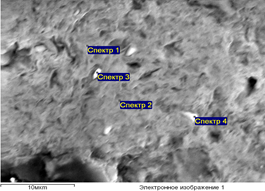
\includegraphics[width=0.8\textwidth]{assets/1043}
	\caption*{}
\end{figure}

а ә

\begin{longtable}[]{@{}
  >{\raggedright\arraybackslash}p{(\columnwidth - 18\tabcolsep) * \real{0.1365}}
  >{\raggedright\arraybackslash}p{(\columnwidth - 18\tabcolsep) * \real{0.1130}}
  >{\raggedright\arraybackslash}p{(\columnwidth - 18\tabcolsep) * \real{0.0926}}
  >{\raggedright\arraybackslash}p{(\columnwidth - 18\tabcolsep) * \real{0.0828}}
  >{\raggedright\arraybackslash}p{(\columnwidth - 18\tabcolsep) * \real{0.0819}}
  >{\raggedright\arraybackslash}p{(\columnwidth - 18\tabcolsep) * \real{0.0952}}
  >{\raggedright\arraybackslash}p{(\columnwidth - 18\tabcolsep) * \real{0.0819}}
  >{\raggedright\arraybackslash}p{(\columnwidth - 18\tabcolsep) * \real{0.0952}}
  >{\raggedright\arraybackslash}p{(\columnwidth - 18\tabcolsep) * \real{0.0680}}
  >{\raggedright\arraybackslash}p{(\columnwidth - 18\tabcolsep) * \real{0.1529}}@{}}
\toprule\noalign{}
\endhead
\bottomrule\noalign{}
\endlastfoot
Спектр & Стат. & O & Mg & Al & Si & Ca & Ti & Fe & Қорытынды \\
1-спектр & Иә & 60.89 & 0.74 & 3.54 & 12.15 & 0.45 & 20.72 & 1.51 &
100.00 \\
2-спектр & Иә & 63.25 & 0.71 & 3.42 & 30.12 & 0.38 & 0.28 & 1.84 &
100.00 \\
3-спектр & Иә & 62,41 & 0.59 & 2,68 & 32.84 & 0.41 & & 1.07 & 100.00 \\
4-спектр & Иә & 62.68 & 0.44 & 2.,38 & 33.65 & & & 0.85 & 100.00 \\
5-спектр & Иә & 56.65 & 1.95 & 9.28 & 26.86 & 0.92 & 0.45 & 3.89 &
100.00 \\
Макс. & & 63.25 & 1.95 & 9.28 & 32.84 & 0.92 & 20.72 & 3.89 & \\
Мин. & & 56.65 & 0.44 & 2.,38 & 12.15 & 0.41 & 0.28 & 0.85 & \\
\end{longtable}

б

\textbf{1-сурет - Бентониттің табиғи түрінің микроқұрылымы (а),
энергодисперсиондық спектрі (ә), элементтік талдауы (б)}

Бентониттердің сорбциялық белсенділігі оларды модификациялау кезінде
жақсарады\emph{.}

\emph{Бентонитті термиялық белсендендіру.} Монтмориллонитті қыздырған
кезде оның суды жоғалтатыны белгілі, бірақ әртүрлі температурада бұл
процесс басқаша жүреді. Әртүрлі кен орындарындағы бентониттердің
сусыздануы олардың түзілу ерекшеліктерімен анықталатын минералогиялық
сипаттамаларына айтарлықтай байланысты {[}4{]}.

Бентониттегі су әртүрлі формада болады: құрылымдық су, адсорбцияланған
су және капиллярлық немесе бос су {[}5{]}. Құрылымдық су немесе
гидроксил түрінде минералдардың құрылымының бөлігі болып табылады және
қатты фазаны 350°C-тан төмен температурада бөлінбейді. Адсорбцияланған
су ішкі және сыртқы беттерде адсорбцияланатын суға сәйкес келеді, яғни
олар агрегаттардың араларындағы кеуектерде (микрокеуектерде) сақталады.
Капиллярлық немесе бос су макрокеуектерде сақталады (2-сур.).

\begin{figure}[H]
	\centering
	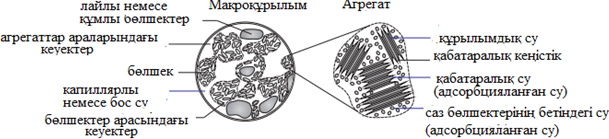
\includegraphics[width=0.8\textwidth]{assets/1044}
	\caption*{}
\end{figure}

\textbf{2-сурет - Бентонит құрылымының концептуалды бейнесі және әртүрлі
суды} \textbf{сақтау механизмдері}

Бентонитті термиялық белсендендіру 200 \textsuperscript{0}С
температурада жүргізілді.

Термиялық жолмен белсендірілген бентонит сазының электрондық
микроскоппен алынған құырылымдық талдауының нәтижелері 3-суретте
келтірілген.

\begin{figure}[H]
	\centering
	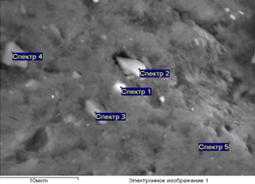
\includegraphics[width=0.8\textwidth]{assets/1045}
	\caption*{}
\end{figure}

\begin{longtable}[]{@{}
  >{\raggedright\arraybackslash}p{(\columnwidth - 18\tabcolsep) * \real{0.1232}}
  >{\raggedright\arraybackslash}p{(\columnwidth - 18\tabcolsep) * \real{0.0841}}
  >{\raggedright\arraybackslash}p{(\columnwidth - 18\tabcolsep) * \real{0.0946}}
  >{\raggedright\arraybackslash}p{(\columnwidth - 18\tabcolsep) * \real{0.0930}}
  >{\raggedright\arraybackslash}p{(\columnwidth - 18\tabcolsep) * \real{0.0930}}
  >{\raggedright\arraybackslash}p{(\columnwidth - 18\tabcolsep) * \real{0.0946}}
  >{\raggedright\arraybackslash}p{(\columnwidth - 18\tabcolsep) * \real{0.0930}}
  >{\raggedright\arraybackslash}p{(\columnwidth - 18\tabcolsep) * \real{0.0930}}
  >{\raggedright\arraybackslash}p{(\columnwidth - 18\tabcolsep) * \real{0.0930}}
  >{\raggedright\arraybackslash}p{(\columnwidth - 18\tabcolsep) * \real{0.1387}}@{}}
\toprule\noalign{}
\begin{minipage}[b]{\linewidth}\raggedright
Спектр
\end{minipage} & \begin{minipage}[b]{\linewidth}\raggedright
Стат.
\end{minipage} & \begin{minipage}[b]{\linewidth}\raggedright
O
\end{minipage} & \begin{minipage}[b]{\linewidth}\raggedright
Mg
\end{minipage} & \begin{minipage}[b]{\linewidth}\raggedright
Al
\end{minipage} & \begin{minipage}[b]{\linewidth}\raggedright
Si
\end{minipage} & \begin{minipage}[b]{\linewidth}\raggedright
Ca
\end{minipage} & \begin{minipage}[b]{\linewidth}\raggedright
Ti
\end{minipage} & \begin{minipage}[b]{\linewidth}\raggedright
Fe
\end{minipage} & \begin{minipage}[b]{\linewidth}\raggedright
Қорытынды
\end{minipage} \\
\midrule\noalign{}
\endhead
\bottomrule\noalign{}
\endlastfoot
1-спектр & Иә & 56.96 & 2.78 & 9.85 & 26.87 & 0.69 & & 2.85 & 100.00 \\
2-спектр & Иә & 57.81 & 2.05 & 9.63 & 25.86 & 0.87 & & 3.78 & 100.00 \\
3-спектр & Иә & 60.05 & 1.88 & 6.97 & 18.79 & 0.65 & 9.65 & 2.01 &
100.00 \\
4-спектр & Иә & 63.23 & 1.73 & 4.36 & 28.01 & 0.80 & & 1,87 & 100.00 \\
Макс. & & 63.23 & 2.78 & 9.85 & 28.01 & 0.87 & 9.65 & 3.78 & \\
Мин. & & 56.96 & 1.73 & 4.36 & 18.86 & 0.65 & 9.65 & 1,87 & \\
\end{longtable}

б

\textbf{3-сурет - Термиялық жолмен белсендірілген бентониттің
микроқұрылымы (а), энергодисперсиондық спектрі (ә) және элементтік
талдау (б) нәтижелері}

Термобелсендендірілген бентониттің микроқұрылымы өзгергені көрініп тұр.
Өңделген бентониттің беткі жағы бұдырлы бетке өзгеріп, кеуектілігі
артқан (3-сурет).

Сазды белсендіру температурасы оның адсорбциялық қасиеттеріне әсер
ететіні көрсетілген {[}6{]}.

Сазды 200\textsuperscript{0}С дейін температурада өңдегенде
коллиодтардың бетінен әлсіз байланысқан су бөлініп, саздың бетіндегі
энергетикалық орталықтар босайды да, саздың адсорбциялық қасиеттері
жақсарады. Саздың құрылымы бұл кезде өзгермейді.

Одан жоғары температурада (t\textgreater400°С) өңдеу саздың құрылымын
өзгертіп, коллоидтың энергетикалық белсенділігін төмендетеді. Сондықтан
саздардың адсорбциялық белсенділігі бірнеше есе төмендейді.

Нәтижесінде қабаттардың арасындағы су бөлініп, бентонит бөлшектері мен
кварц түйірлері арасында қашықтық азаяды, электростатикалық тартылыс
күштері артып, бентонит бөлшектерінің бағытталуын жақсартады.

Термиялық өңдеу бентониттің ортасынан бос және құрылымдық суды жойып,
қыздырудың бастапқы кезінде кеуектерді түзеді. Бірақ одан ары қарай
температураны арттыру және уақытын көбейту бентониттің құрылымының
жойылуына және оның беткі ауданын азайтуға әкелуі мүмкін.

Термиялық белсендендіру кезінде кварцтың мөлшері артатыны анықталған
{[}7{]}. Ол бентонит құрамынан қоспалардың және судың бөлінуінен
байқалуы тиіс. Бұл қыздыру кезінде саздан кварцты жоюға болмайтынын
көрсетеді.

Үлгілерді белсендендірудің алдында қатты қыздыру құрылымдық
параметрлерінің біршама өзгеруіне әкеледі. Бұл дегидратация, бентониттің
дисперстлігі, меншікті бетінің өсуімен байланысты. Мүмкін, сазда
температураның және ылғалдың әсерінен саздағы «бітелген кеуектердің» бір
бөлігі ашылып, жеке бөлімдері бұзылып, бір-бірімен жанасатын кеуектердің
жалпы жүйесіне ендіріледі.

Химиялық өңдеу құрылымының өзгеруіне, алмасатын катиондардың құрамы
өзгеруіне және жаңа белсенді орталықтардың пайда болуына байланысты
ионалмасу қасиеттерінің артуына әкеледі. Бентонитті белсендендіру
әдісінің бірі ол жоғары температурадағы қышқылдық белсендендіру болып
табылады.

Термоқышқылдық белсендендіруді өткен бентониттің құрылымдық талдау
нәтижелері 4-суретте көрсетілген.

\begin{figure}[H]
	\centering
	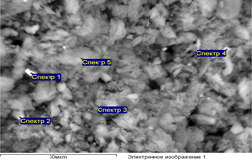
\includegraphics[width=0.8\textwidth]{assets/1046}
	\caption*{}
\end{figure}

\begin{longtable}[]{@{}
  >{\raggedright\arraybackslash}p{(\columnwidth - 26\tabcolsep) * \real{0.1168}}
  >{\raggedright\arraybackslash}p{(\columnwidth - 26\tabcolsep) * \real{0.0703}}
  >{\raggedright\arraybackslash}p{(\columnwidth - 26\tabcolsep) * \real{0.0706}}
  >{\raggedright\arraybackslash}p{(\columnwidth - 26\tabcolsep) * \real{0.0597}}
  >{\raggedright\arraybackslash}p{(\columnwidth - 26\tabcolsep) * \real{0.0597}}
  >{\raggedright\arraybackslash}p{(\columnwidth - 26\tabcolsep) * \real{0.0597}}
  >{\raggedright\arraybackslash}p{(\columnwidth - 26\tabcolsep) * \real{0.0706}}
  >{\raggedright\arraybackslash}p{(\columnwidth - 26\tabcolsep) * \real{0.0597}}
  >{\raggedright\arraybackslash}p{(\columnwidth - 26\tabcolsep) * \real{0.0597}}
  >{\raggedright\arraybackslash}p{(\columnwidth - 26\tabcolsep) * \real{0.0597}}
  >{\raggedright\arraybackslash}p{(\columnwidth - 26\tabcolsep) * \real{0.0597}}
  >{\raggedright\arraybackslash}p{(\columnwidth - 26\tabcolsep) * \real{0.0597}}
  >{\raggedright\arraybackslash}p{(\columnwidth - 26\tabcolsep) * \real{0.0597}}
  >{\raggedright\arraybackslash}p{(\columnwidth - 26\tabcolsep) * \real{0.1343}}@{}}
\toprule\noalign{}
\begin{minipage}[b]{\linewidth}\raggedright
Спектр
\end{minipage} & \begin{minipage}[b]{\linewidth}\raggedright
Стат.
\end{minipage} & \begin{minipage}[b]{\linewidth}\raggedright
O
\end{minipage} & \begin{minipage}[b]{\linewidth}\raggedright
Na
\end{minipage} & \begin{minipage}[b]{\linewidth}\raggedright
Mg
\end{minipage} & \begin{minipage}[b]{\linewidth}\raggedright
Al
\end{minipage} & \begin{minipage}[b]{\linewidth}\raggedright
Si
\end{minipage} & \begin{minipage}[b]{\linewidth}\raggedright
S
\end{minipage} & \begin{minipage}[b]{\linewidth}\raggedright
Cl
\end{minipage} & \begin{minipage}[b]{\linewidth}\raggedright
Ca
\end{minipage} & \begin{minipage}[b]{\linewidth}\raggedright
Ti
\end{minipage} & \begin{minipage}[b]{\linewidth}\raggedright
Fe
\end{minipage} & \begin{minipage}[b]{\linewidth}\raggedright
Ba
\end{minipage} & \begin{minipage}[b]{\linewidth}\raggedright
Қорытынды
\end{minipage} \\
\midrule\noalign{}
\endhead
\bottomrule\noalign{}
\endlastfoot
1-спектр & Иә & 50.42 & & 0.84 & 8,97 & 17.37 & 4.56 & & & & 2.44 & 15.4
& 100.00 \\
1-спектр & Иә & 62.09 & & 1.10 & 6.05 & 11.52 & & & 0.19 & 14.0 & 5.05 &
& 100.00 \\
1-спектр & Иә & 61.22 & 0.31 & 1.15 & 9.09 & 23.47 & & 0.15 & 0.21 &
0.35 & 4.05 & & 100.00 \\
1-спектр & Иә & 63.77 & 0.67 & 0.74 & 7.26 & 24.71 & & & 0.15 & 0.25 &
2.45 & & 100.00 \\
1-спектр & Иә & 64.41 & 0.57 & 0.84 & 6.56 & 25.09 & & 0.16 & 0.29 & &
2.08 & & 100.00 \\
Макс. & & 64.41 & 0.67 & 1.15 & 9.09 & 25.09 & 4.56 & 0.16 & 0.22 & 14.0
& 5.05 & 15.4 & \\
Мин. & & 50.42 & 0.31 & 0.74 & 6.56 & 11.50 & 4.56 & 0.15 & 0.15 & 0.25
& 2.08 & 15.4 & \\
\end{longtable}

б

\textbf{4-сурет - Термоқышқылдық жолмен белсендендірілген бентониттің
микроқұрылымы (а), энергодисперсиондық спектрі (ә), элементтік талдау
(б) нәтижелері}

Термоқышқылдық әдіспен белсендірілген түрінде бентониттің
микроқұрылымының елеулі өзгергені, беті бос, кеуекті және қабыршақты
болатыны көрінеді.

Бентонитті қышқылдық белсендіру үлгідегі магний, темір, сілтілі және
сілтілікжер металдардың оксидтері мөлшерінің азаюуына әкеледі, себебі
бұл процесс кезінде металдардың оксидтері шайылады.

Бентониттерді қышқылдық белсендіру кезінде \emph{Na\textsuperscript{+},
K\textsuperscript{+}, Ca\textsuperscript{2+}, Mg\textsuperscript{2+}}
иондарын сутек иондарына алмастырудан басқа монтмориллониттің кристалдық
құрылымы бұзылады. Алмасуға қабілетті \emph{Н\textsuperscript{+}} және
\emph{Al\textsuperscript{3+ }}катиондары түзіледі және алмасатын
алюминий катиондары сутек катиондарынан көбірек болады.

Термоқышқылды белсендіру кезінде сілтілікжер металдардың иондарын
ығыстыратын ион - сутек катионы H\textsuperscript{+} болады. Сулы ортада
ең аз мөлшеріне байланысты ең үлкен қозғалғыштығы бар ион алмасу
процесінде протон кальций мен магний иондарының қосымша мөлшерін
жылжымалы түрге айналдыра отырып, материалдың ион алмасу қабілетін
барынша арттыруы тиіс {[}8{]}.

Бентонит саздарын қышқылдық активтендіру кезінде тек октаэдрлік
(орталық) қабаты ғана емес, монтмориллонит торының тетраэдрлік қабаттары
да бұзылады. Бұл тетраэдрлік

және октаэдрлік қабаттардағы изоморфты алмастырулар санының азаюымен
дәлелденеді.

Монтмориллонит құрылымынан алынған алюминий иондарының қалған бөлігі
магний мен темір иондарын алмасу орындарынан ығыстырып, оның теріс
зарядтарының орнын толтыру үшін тормен байланысады және
Н\textsuperscript{+} иондарымен бірге алмасатын қышқылдығын
(H\textsuperscript{+}+Al\textsuperscript{3+}) негіздейді.

\emph{Бентонитті қолдана отырып ағынды суларды тазарту.}

Зерттеуге алынған Шығыс-Қазақстан облысындағы Белоус полиметалл кен
орынының шахта суларының сипаттамасы төменде 3-кестеде келтірілген.

\textbf{3-кесте - Шығыс-Қазақстан облысындағы Белоус полиметалл кен
орынының шахта суларының сипаттамасы (рН 7,1÷7,6)}

% \begin{longtable}[]{@{}
%   >{\raggedright\arraybackslash}p{(\columnwidth - 4\tabcolsep) * \real{0.2827}}
%   >{\raggedright\arraybackslash}p{(\columnwidth - 4\tabcolsep) * \real{0.3838}}
%   >{\raggedright\arraybackslash}p{(\columnwidth - 4\tabcolsep) * \real{0.3334}}@{}}
% \toprule\noalign{}
% \endhead
% \bottomrule\noalign{}
% \endlastfoot
% \multirow{2}{*}{Компоненттер} & \multicolumn{2}{l@{}}{%
% Компоненттің мөлшері, мг/дм\textsuperscript{3}} \\
% & тұнбада & фильтратта \\
% Cu\textsuperscript{2+} & 8,20\begin{figure}[H]
% 	\centering
% 	
\includegraphics[width=0.8\textwidth]{assets/1047}
% 	\caption*{}
% \end{figure}0,20 &
% 0,21\begin{figure}[H]
% 	\centering
% 	
\includegraphics[width=0.8\textwidth]{assets/1047}
% 	\caption*{}
% \end{figure}0,04 \\
% Pb\textsuperscript{2+} & 4,80\begin{figure}[H]
% 	\centering
% 	
\includegraphics[width=0.8\textwidth]{assets/1047}
% 	\caption*{}
% \end{figure}0,16 &
% 0,11\begin{figure}[H]
% 	\centering
% 	
\includegraphics[width=0.8\textwidth]{assets/1047}
% 	\caption*{}
% \end{figure}0,03 \\
% Cd\textsuperscript{2+} & 0,25\begin{figure}[H]
% 	\centering
% 	
\includegraphics[width=0.8\textwidth]{assets/1047}
% 	\caption*{}
% \end{figure}0,02 &
% 0,17\begin{figure}[H]
% 	\centering
% 	
\includegraphics[width=0.8\textwidth]{assets/1047}
% 	\caption*{}
% \end{figure}0,02 \\
% Zn\textsuperscript{2+} & 67,10\begin{figure}[H]
% 	\centering
% 	
\includegraphics[width=0.8\textwidth]{assets/1047}
% 	\caption*{}
% \end{figure}0,63 &
% 12,3\begin{figure}[H]
% 	\centering
% 	\includegraphics[width=0.8\textwidth]{assets/1047}
% 	\caption*{}
% \end{figure}0,39 \\
% Жүзгін заттар & 260,00 & 50,00 \\
% \end{longtable}

Ауыр металдардың сазбен сорбциялануы негізінен екі механизм арқылы
жүреді: ион алмасу (монтмориллониттің қабат аралық кеңістіктерінде
орналасқан катиондардың алмасуы) және минералдың беткі гидроксил
топтарымен хелаттық кешендердің түзілуі. Табиғи минералдың құрамына
байланысты сорбция процесінің механизмі әртүрлі болуы мүмкін {[}9-11{]}.

Ион алмасумен қатар бентонит саздарында физикалық және молекулалық
сорбция жүруі мүмкін. Физикалық сорбция иондануға қабілетті қышқылдық
және негіздік сипаттағы кристалдық беттер мен беттік гидроксид
топтарында артық теріс зарядтың болуына байланысты.

Молекулалық сорбция кезінде қабаттар арасында сорбцияланған заттар
орналасады, қабаттардың құрылымын өзгертпейді. Осылайша, мұндай белсенді
орталықтар - алмасатын катиондары, гидроксил топтары, бентонит
саздарының активтенуі осы сорбенттердің практикалық қолданысын
арттырады.

\begin{figure}[H]
	\centering
	\includegraphics[width=0.8\textwidth]{assets/1048}
	\caption*{}
\end{figure}

а ә

\begin{longtable}[]{@{}
  >{\raggedright\arraybackslash}p{(\columnwidth - 26\tabcolsep) * \real{0.1130}}
  >{\raggedright\arraybackslash}p{(\columnwidth - 26\tabcolsep) * \real{0.0436}}
  >{\raggedright\arraybackslash}p{(\columnwidth - 26\tabcolsep) * \real{0.0527}}
  >{\raggedright\arraybackslash}p{(\columnwidth - 26\tabcolsep) * \real{0.0644}}
  >{\raggedright\arraybackslash}p{(\columnwidth - 26\tabcolsep) * \real{0.0653}}
  >{\raggedright\arraybackslash}p{(\columnwidth - 26\tabcolsep) * \real{0.0654}}
  >{\raggedright\arraybackslash}p{(\columnwidth - 26\tabcolsep) * \real{0.0645}}
  >{\raggedright\arraybackslash}p{(\columnwidth - 26\tabcolsep) * \real{0.0645}}
  >{\raggedright\arraybackslash}p{(\columnwidth - 26\tabcolsep) * \real{0.0654}}
  >{\raggedright\arraybackslash}p{(\columnwidth - 26\tabcolsep) * \real{0.0668}}
  >{\raggedright\arraybackslash}p{(\columnwidth - 26\tabcolsep) * \real{0.0727}}
  >{\raggedright\arraybackslash}p{(\columnwidth - 26\tabcolsep) * \real{0.0549}}
  >{\raggedright\arraybackslash}p{(\columnwidth - 26\tabcolsep) * \real{0.0654}}
  >{\raggedright\arraybackslash}p{(\columnwidth - 26\tabcolsep) * \real{0.1415}}@{}}
\toprule\noalign{}
\begin{minipage}[b]{\linewidth}\raggedright
Спектр
\end{minipage} & \begin{minipage}[b]{\linewidth}\raggedright
Стат.
\end{minipage} & \begin{minipage}[b]{\linewidth}\raggedright
О
\end{minipage} & \begin{minipage}[b]{\linewidth}\raggedright
Mg
\end{minipage} & \begin{minipage}[b]{\linewidth}\raggedright
Al
\end{minipage} & \begin{minipage}[b]{\linewidth}\raggedright
Si
\end{minipage} & \begin{minipage}[b]{\linewidth}\raggedright
S
\end{minipage} & \begin{minipage}[b]{\linewidth}\raggedright
Ca
\end{minipage} & \begin{minipage}[b]{\linewidth}\raggedright
Ti
\end{minipage} & \begin{minipage}[b]{\linewidth}\raggedright
Fe
\end{minipage} & \begin{minipage}[b]{\linewidth}\raggedright
Zn
\end{minipage} & \begin{minipage}[b]{\linewidth}\raggedright
Co
\end{minipage} & \begin{minipage}[b]{\linewidth}\raggedright
Ba
\end{minipage} & \begin{minipage}[b]{\linewidth}\raggedright
Қорытынды
\end{minipage} \\
\midrule\noalign{}
\endhead
\bottomrule\noalign{}
\endlastfoot
1-спектр & Иә & 42.03 & & 5.35 & 10.57 & 5.42 & 0.38 & & 2.06 & 11.02 &
0.0 & 23.14 & 100.00 \\
2-спектр & Иә & 56.97 & 0.76 & 5.54 & 10.99 & & 0.66 & 21.77 & 3.31 & &
& & 100.00 \\
3-спектр & Иә & 43.56 & 0.88 & 3.82 & 16.00 & & 0.56 & & 35.18 & & & &
100.00 \\
4-спектр & Иә & 54.86 & 1.85 & 10.96 & 25.76 & & 0.87 & 0.72 & 4.98 & &
& & 100.00 \\
5-спектр & Иә & 55.65 & 1.49 & 10.49 & 26.88 & & 0.80 & & 4.69 & & & &
100.00 \\
Макс. & & 56.97 & 1.85 & 10.96 & 26.88 & 5.42 & 0.87 & 21.77 & 35.18 &
11.02 & 0.0 & 23.14 & \\
Мин. & & 42.06 & 0.76 & 3.82 & 10.57 & 5.42 & 0.38 & 0.72 & 2.06 & 11.02
& 0.0 & 23.14 & \\
\end{longtable}

\emph{Барлық нәтижелер массалық \%}

\textbf{5-сурет - Термоқышқылдық жолмен белсендірілген бентонит сазының
микроқұрылымы (а), энергодисперсиондық спектрі (ә), элементтік талдау
нәтижелері (в)}

\textbf{ағынды сумен әрекеттескеннен кейін}

Термоқышқылдық жолмен белсендірілген бентонит сазының ағынды сумен
жанасқаннан кейін құрамында сілтілі және сілтілі жер металдарының
катиондары ғана емес, сонымен қатар, құрамындағы қоспалар да бар, майда
кристалды құрылымы бар тығыз материал түзіледі (5-сурет). Көрсетілген
нәтиже мырыш элементінің бар екендігін көрсетеді. Бұл термоқышқылды
жолмен белсендірілген түрдегі бентониттің ағынды сумен байланысқаннан
кейін мырыш иондарының сорбцияланғанын дәлелдейді.

Ағынды суларды ауыр металдар иондарынан (\emph{Cu\textsuperscript{2+},
Pb\textsuperscript{2+}, Cd\textsuperscript{2+}, Zn\textsuperscript{2+}})
бентониттің түрлі формаларымен тазарту нәтижелерін салыстыру төмендегі
4-кестеде келтірілген.

\textbf{4-кесте - Табиғи және термиялық қышқылмен белсендірілген
бентонитті пайдалана отырып, шахта суынан ауыр металл иондарын алу}

\begin{longtable}[]{@{}
  >{\raggedright\arraybackslash}p{(\columnwidth - 8\tabcolsep) * \real{0.1616}}
  >{\raggedright\arraybackslash}p{(\columnwidth - 8\tabcolsep) * \real{0.1394}}
  >{\raggedright\arraybackslash}p{(\columnwidth - 8\tabcolsep) * \real{0.2271}}
  >{\raggedright\arraybackslash}p{(\columnwidth - 8\tabcolsep) * \real{0.2272}}
  >{\raggedright\arraybackslash}p{(\columnwidth - 8\tabcolsep) * \real{0.2447}}@{}}
\toprule\noalign{}
\multirow{3}{*}{\begin{minipage}[b]{\linewidth}\raggedright
Металдардың иондары
\end{minipage}} &
\multicolumn{4}{>{\raggedright\arraybackslash}p{(\columnwidth - 8\tabcolsep) * \real{0.8384} + 6\tabcolsep}@{}}{%
\begin{minipage}[b]{\linewidth}\raggedright
Бентонит
\end{minipage}} \\
&
\multicolumn{4}{>{\raggedright\arraybackslash}p{(\columnwidth - 8\tabcolsep) * \real{0.8384} + 6\tabcolsep}@{}}{%
\begin{minipage}[b]{\linewidth}\raggedright
Иондырдың сіңірілуі, \%
\end{minipage}} \\
& \begin{minipage}[b]{\linewidth}\raggedright
\begin{quote}
табиғи
\end{quote}
\end{minipage} & \begin{minipage}[b]{\linewidth}\raggedright
қышқылмен белсендірілген
\end{minipage} & \begin{minipage}[b]{\linewidth}\raggedright
термиялық жолмен белсендірілген
\end{minipage} & \begin{minipage}[b]{\linewidth}\raggedright
термоқышқылды жолмен белсендірілген
\end{minipage} \\
\midrule\noalign{}
\endhead
\bottomrule\noalign{}
\endlastfoot
Cu \textsuperscript{2+} & 15,1 & 16,2 & 25,7 & 96,4 \\
Pb\textsuperscript{2+} & 78,7 & 91,4 & 83,5 & 98,2 \\
Cd\textsuperscript{2+} & 26,2 & 48,7 & 39,5 & 94,1 \\
Zn\textsuperscript{2+} & 96,3 & 34,8 & 97,2 & 98,6 \\
\end{longtable}

Алынған нәтижелерден көрініп тұрғандай, қышқылдық активтенуден өткен
бентонит сазын алдын ала термиялық өңдеусіз қолданғанда, ауыр металдар
иондарының экстракциялану дәрежесі термиялық активтендірілген немесе
термоқышқылды белсендірілген формаларды пайдаланғанға қарағанда төмен
(4-кесте). Мұның себептері пайдаланылған үлгінің ісінуіне байланысты
болуы, сонымен қатар, зерттелетін катиондар ғана емес, басқа да полярлы
органикалық және бейорганикалық қосылыстардың молекулалары ауыр металдар
иондарымен бәсекелесіп, аралық кеңістікке еніп кетуі мүмкіндігіне
байланысты.

Шахта суын тазартуда термиялық және қышқылмен белсендірілген бентонитті
(200 \textsuperscript{0}С температурада -4 сағат, содан кейін 4 сағат
бойы 10\% H\textsubscript{2}SO\textsubscript{4} өңдеу) пайдалану ауыр
металдары иондарының толықтай дерлік экстракциялануын қамтамасыз етеді
Cu\textsuperscript{2+}, Pb\textsuperscript{2+}, Cd\textsuperscript{2+},
Zn\textsuperscript{2+} (сәйкес 96,4 ; 98,2; 94,1; 98,6\%).

\textbf{5-кесте - Түрлі бентонит формаларымен тазартылған ағынды судағы
ауыр металдар иондарының концентрациясы}

\begin{longtable}[]{@{}
  >{\raggedright\arraybackslash}p{(\columnwidth - 10\tabcolsep) * \real{0.1682}}
  >{\raggedright\arraybackslash}p{(\columnwidth - 10\tabcolsep) * \real{0.1826}}
  >{\raggedright\arraybackslash}p{(\columnwidth - 10\tabcolsep) * \real{0.1226}}
  >{\raggedright\arraybackslash}p{(\columnwidth - 10\tabcolsep) * \real{0.1600}}
  >{\raggedright\arraybackslash}p{(\columnwidth - 10\tabcolsep) * \real{0.1721}}
  >{\raggedright\arraybackslash}p{(\columnwidth - 10\tabcolsep) * \real{0.1945}}@{}}
\toprule\noalign{}
\multirow{3}{*}{\begin{minipage}[b]{\linewidth}\raggedright
Металдардың иондары
\end{minipage}} &
\multicolumn{5}{>{\raggedright\arraybackslash}p{(\columnwidth - 10\tabcolsep) * \real{0.8318} + 8\tabcolsep}@{}}{%
\begin{minipage}[b]{\linewidth}\raggedright
Ауыр металдар иондарының концентрациясы, \emph{мг/дм\textsuperscript{3}}
\end{minipage}} \\
& \multirow{2}{*}{\begin{minipage}[b]{\linewidth}\raggedright
Тазартылмаған суда, С
\end{minipage}} &
\multirow{2}{*}{\begin{minipage}[b]{\linewidth}\raggedright
ШРК\textsubscript{б-ш.}
\end{minipage}} &
\multicolumn{3}{>{\raggedright\arraybackslash}p{(\columnwidth - 10\tabcolsep) * \real{0.5266} + 4\tabcolsep}@{}}{%
\begin{minipage}[b]{\linewidth}\raggedright
Тазартылған шахта суында
\end{minipage}} \\
& & & \begin{minipage}[b]{\linewidth}\raggedright
табиғи

бентонитпен, С\textsubscript{б}
\end{minipage} & \begin{minipage}[b]{\linewidth}\raggedright
термиялық

белсендірілген бентонитпен, С\textsubscript{т}
\end{minipage} & \begin{minipage}[b]{\linewidth}\raggedright
термоқышқылды

белсендірілген бентонитпен, С\textsubscript{тқ}
\end{minipage} \\
\midrule\noalign{}
\endhead
\bottomrule\noalign{}
\endlastfoot
Cu\textsuperscript{2+} & 0,21 & 0,001 & 0,1 & 0,07 & 0,001 \\
Pb\textsuperscript{2+} & 0,11 & 0,10 & 0,09 & 0,03 & 0,010 \\
Cd\textsuperscript{2+} & 0,17 & 0,005 & 0,14 & 0,09 & 0,006 \\
Zn\textsuperscript{2+} & 12,3 & 0,01 & 8,70 & 4,03 & 0,010 \\
\end{longtable}

6-кестеде әртүрлі формадағы бентонит сазымен ағынды сулардан ауыр
металдар иондарын сорбциялау нәтижелері: табиғи, термикалық
белсендірілген, термиялық қышқылмен белсендірілген, сондай-ақ олардың
бастапқы, тазартылған ағынды сулардың концентрациясының қатынасы ретінде
салыстырмалы деректері келтірілген.

\textbf{6-кесте - Шаруашылық қызмет үшін судағы осы иондардың шекті
рұқсат етілген концентрацияларымен (ШРК) салыстырғанда ауыр металл
иондарын}

\textbf{бентонит сазымен сіңіру}

\begin{longtable}[]{@{}
  >{\raggedright\arraybackslash}p{(\columnwidth - 12\tabcolsep) * \real{0.1595}}
  >{\raggedright\arraybackslash}p{(\columnwidth - 12\tabcolsep) * \real{0.1159}}
  >{\raggedright\arraybackslash}p{(\columnwidth - 12\tabcolsep) * \real{0.1159}}
  >{\raggedright\arraybackslash}p{(\columnwidth - 12\tabcolsep) * \real{0.1594}}
  >{\raggedright\arraybackslash}p{(\columnwidth - 12\tabcolsep) * \real{0.1450}}
  >{\raggedright\arraybackslash}p{(\columnwidth - 12\tabcolsep) * \real{0.1594}}
  >{\raggedright\arraybackslash}p{(\columnwidth - 12\tabcolsep) * \real{0.1449}}@{}}
\toprule\noalign{}
\multirow{3}{*}{\begin{minipage}[b]{\linewidth}\raggedright
Ауыр металл иондарының концентрациясы
\end{minipage}} & \multicolumn{6}{l@{}}{%
\begin{minipage}[b]{\linewidth}\raggedright
Ауыр металл иондарының концентрациясы, мг/дм\textsuperscript{3}
\end{minipage}} \\
& \multirow{2}{*}{\begin{minipage}[b]{\linewidth}\raggedright
тазартылмаған суда, С\textsubscript{0}
\end{minipage}} &
\multirow{2}{*}{\begin{minipage}[b]{\linewidth}\raggedright
ШРК\textsubscript{б-ш.}
\end{minipage}} &
\multirow{2}{*}{\begin{minipage}[b]{\linewidth}\raggedright
С\textsubscript{0}/ШРК\textsubscript{б-ш.}
\end{minipage}} & \multicolumn{3}{l@{}}{%
\begin{minipage}[b]{\linewidth}\raggedright
Ауыр металдар иондарының концентрациясының тазартылғаннан кейін
ШРК\textsubscript{б-ш.} қатынасы
\end{minipage}} \\
& & & & \begin{minipage}[b]{\linewidth}\raggedright
С\textsubscript{и}/ШРК\textsubscript{б-ш.}
\end{minipage} & \begin{minipage}[b]{\linewidth}\raggedright
С\textsubscript{т} /ШРК\textsubscript{б.-ш.}
\end{minipage} & \begin{minipage}[b]{\linewidth}\raggedright
С\textsubscript{тк}/ ШРК\textsubscript{б-ш.}
\end{minipage} \\
\midrule\noalign{}
\endhead
\bottomrule\noalign{}
\endlastfoot
Cu \textsuperscript{2+} & 0,21 & 0,001 & 210 & 140 & 70 & 1,0 \\
Pb\textsuperscript{2+} & 0,11 & 0,10 & 1,1 & 0,9 & 0,3 & 0,1 \\
Cd\textsuperscript{2+} & 0,17 & 0,005 & 34 & 38,0 & 4,5 & 1,2 \\
Zn\textsuperscript{2+} & 12,3 & 0,01 & 1230 & 870 & 40,3 & 1,0 \\
\end{longtable}

Берілген арақатынастарды С\textsubscript{б}/ШРК\textsubscript{б.-ш.,}
С\textsubscript{т}/ШРК\textsubscript{б.-ш.,}
С\textsubscript{тк}/ШРК\textsubscript{б.-ш.,} ауыр металдарды саздың әр
түрлі формалары: табиғи, термиялық және термоқышқылдық жолмен
белсендірілген бентонитті қолданғанда, зерттелетін иондарға қатысты ең
жақсы сорбент термоқышқылды белсендірілген бентонит екенін көрсетеді.

7-кестеде зерттеу нәтижелерінің метрологиялық сипаттамалары берілген.

\textbf{7-кесте - Зерттеу нәтижелерін метрологиялық бағалау}

\textbf{(конвергенция, қайталану және дәлдіктің стандартты ауытқуы)}

\begin{longtable}[]{@{}
  >{\raggedright\arraybackslash}p{(\columnwidth - 6\tabcolsep) * \real{0.2959}}
  >{\raggedright\arraybackslash}p{(\columnwidth - 6\tabcolsep) * \real{0.2440}}
  >{\raggedright\arraybackslash}p{(\columnwidth - 6\tabcolsep) * \real{0.2258}}
  >{\raggedright\arraybackslash}p{(\columnwidth - 6\tabcolsep) * \real{0.2343}}@{}}
\toprule\noalign{}
\endhead
\bottomrule\noalign{}
\endlastfoot
Ауыр металдардың иондары & S\textsubscript{сх.} ·10\textsuperscript{4} &
S\textsubscript{қайт.} ·10\textsuperscript{4} & S\textsubscript{дұр.}
·10\textsuperscript{4} \\
Cu\textsuperscript{2+} & 1,81 & 2,95 & 1,25 \\
Cd\textsuperscript{2+} & 1,92 & 2,89 & 2,52 \\
Pb\textsuperscript{2+} & 2,69 & 5,35 & 1,83 \\
Zn\textsuperscript{2+} & 15,9 & 25,3 & 23,5 \\
\end{longtable}

Алынған зерттеу нәтижелері бойынша есептелген метрологиялық сипаттамалар
(қайталанудың стандартты ауытқуларының мәні, нәтижелердің
дұрыстығын/дәлдігін бақылау) (7 кесте) зерттелетін барлық металл иондары
(Cu\textsuperscript{2+}, Cd\textsuperscript{2+}, Pb\textsuperscript{2+},
Zn\textsuperscript{2+}) үшін жүйелі қателер бойынша статистикалық
маңызды емес.

\textbf{Қорытынды.} Эксперименттік зерттеулер нәтижесі бойынша:

- Шығыс Қазақстан облысындағы Белоусов полиметалл кен орнының шахта
суларынан ауыр металл иондарының Шығыс Қазақстан облысы Таған кен
орнының 14 горизонтындағы үш түрлі модификацияда: табиғи, қышқылды
активтендірілген және термоқышқылды белсендірілген бентонит сазымен
адсорбциясы туралы мәліметтер алынды;

- бастапқы ағынды сулардың концентрациясының тазартылған ағынды суларға
қатынасы шекті рұқсат етілген концентрация мәндерімен салыстыра
зерттелді;

- зерттелетін иондарға қатысты ең тиімді сорбент бентонит сазының
термоқышқылды белсендірілген түрі болатыны анықталды;

- бірқатар тәжірибелер негізінде оңтайлы жағдайларда термоқышқылды
жолмен белсендірілген бентонит сазы ағынды сулардан
Cu\textsuperscript{2+}, Pb\textsuperscript{2+}, Cd\textsuperscript{2+},
Zn\textsuperscript{2+} иондарын тиісінше 99,6, 94,7, 98,9 және 99,5\%-ға
жоюға, мүмкіндік беретіні анықталды. Бұл балық шаруашылығы үшін арналған
суларға шектеулі рұқсат етілген концентрациялары мәндеріне сәйкес
келеді.

\emph{\textbf{Қаржыландыру}.} Бұл ғылыми зерттеу IRN AP19674742 «Шығыс
Қазақстанның табиғи бентониті негізінде жаңа органикалық минералды
композициялық материалды алу технологиясы» жобасын гранттық қаржыландыру
шеңберінде жүзеге асырылды. Қаржыландыру көзі -- Қазақстан Республикасы
Ғылым және жоғары білім министрлігінің Ғылым комитеті.

\textbf{Әдебиеттер}

1.Сапаргалиев Е.М. Влияние вещественного состава сырья на
технологические свойства бентонитов Таганского месторождения //Вестник
РУДН. Серия инженерные исследования. - 2007. -№2. -C. 77-81

2. Shamkhanov M.Ch. Adsorbenty na osnove prirodnogo bentonita //Vestnik
magistratury. -2021. -№ 5 (116). -S. 34-37

3. Dieudonne A.C. Microstructure of bentonites: characterisation and
evolution under mechanical and environmental loads //EURAD School for
Radioactive Waste Management. Belgium. -2020, -P. 1-21.

4. Горюшкин В.В. Технологические свойства бентонитов палеоцена
воронежской антеклизы и возможности их изменения // Вестник воронежского
университета. Геология. -2005. -№ 1. -C. 166-177

5.Jacinto A. C., Villar, Ledesma M. V. Influence of water density on the
water-retention curve of expansive clays// Geotechnique. -2012. -№
8(62). -P. 657-667.

6.Анюхина А.В., Середин В.В., Андрианов А.В., Хлуденева Т.Ю. Влияние
термической обработки глин на их адсорбцию по красителю метиленовый
голубой // Недропользование. -2021. -Т. 21. -№ 2. -С.52-57. DOI
10.15593/2712-8008/2021.2.1

7.Amari A., Chlendi M., Gannouni A., Bellagi A. Optimised activation of
bentonite for toluene adsorption // Applied Clay Science. -2010. -№47.
--P:447-461

8.Burakov A.E., Galunin EV, Burakova IV, Kucherova AE, Agarwal S,
Tkachev A.G., Gupta V.K. Adsorption of heavy metals on conventional and
nanostructured materials for wastewater treatment purposes: A review//
Ecotoxicology and Environmental Safety. -2018.-№148, -P.702--712. DOI
10.1016/j.ecoenv.2017.11.034.

9.Кошелев А. В., Веденеева Н. В., Заматырина В. А., Тихомирова Е. И.,
Скиданов Е. В. Разработка технологии получения сорбентов на основе
бентонитовых глин для систем очистки воды // Вода и экология: проблемы и
решения. -2018. -№ 2 (74), - C. 32-39 DOI
10.23968/2305--3488.2018.20.2.32--39

10. Bourliva A., Michailidis K, Sikalidis C, Filippidis A, Betsiou M.
Adsorption of Cd(II), Cu(II), Ni(II) and Pb(II) on to natural bentonite:
study in mono- and multi- metal systems // Environ Earth Sci. - 2015.
--Vol. 73. --P. 5435--5444. DOI 10.1007/s12665-014-3798-0 11.Черкасов
А.С., Сомин В.А., Комарова Л.Ф., Куртукова Л.В. Изучение сорбционных
свойств бентонита милосского месторождения и материала на его основе //
Ползуновский вестник. - 2014. - №3. с. 254-256

\textbf{References}

1. Sapargaliev E.M. Vliyanie veshchestvennogo sostava
syr\textquotesingle ya na tekhnologicheskie svoistva bentonitov
Taganskogo mestorozhdeniya //Vestnik RUDN. Seriya inzhenernye
issledovaniya. - 2007. -№2. -S. 77-81 {[}in Russian{]}

2. Shamkhanov M.Ch. Adsorbenty na osnove prirodnogo bentonita //Vestnik
magistratury.//-2021. -№ 5 (116). -S. 34-37. {[}in Russian{]}

3. Dieudonne A.C. Microstructure of bentonites: characterisation and
evolution under mechanical and environmental loads //EURAD School for
Radioactive Waste Management. Belgium. -2020, -P. 1-21

4. Goryushkin V.V. Tekhnologicheskie svoistva bentonitov paleotsena
voronezhskoi anteklizy i vozmozhnosti ikh izmeneniya // Vestnik
voronezhskogo universiteta. Geologiya. -2005. -№ 1. -S. 166-177. {[}in
Russian{]}

5. Jacinto A. C., Villar, Ledesma M. V. Influence of water density on
the water-retention curve of expansive clays// Geotechnique. -2012. -№
8(62). -P. 657-667.

6. Anyukhina A.V., Seredin V.V., Andrianov A.V., Khludeneva T.Yu.
Vliyanie termicheskoi obrabotki glin na ikh adsorbtsiyu po krasitelyu
metilenovyi goluboi // Nedropol\textquotesingle zovanie. -2021. -T. 21.
-№ 2, -S.52-57. DOI 10.15593/2712-8008/2021.2.1 {[}in Russian{]}

7. Amari A., Chlendi M., Gannouni A., Bellagi A. Optimised activation of
bentonite for toluene adsorption // Applied Clay Science. -2010. -№47.
--P:447-461

8. Burakov A.E., Galunin EV, Burakova IV, Kucherova AE, Agarwal S,
Tkachev A.G., Gupta V.K. Adsorption of heavy metals on conventional and
nanostructured materials for wastewater treatment purposes: A review//
Ecotoxicology and Environmental Safety. -2018. -№148. -P.702--712. DOI
10.1016/j.ecoenv.2017.11.034.

9. Koshelev A. V., Vedeneeva N. V., Zamatyrina V. A., Tikhomirova E. I.,
Skidanov E. V. Razrabotka tekhnologii polucheniya sorbentov na osnove
bentonitovykh glin dlya sistem ochistki vody // Voda i ehkologiya:
problemy i resheniya. -2018. -№ 2 (74), - S.32-39 DOI
10.23968/2305--3488.2018.20.2.32--39 {[}in Russian{]}

10. Bourliva A., Michailidis K, Sikalidis C, Filippidis A, Betsiou M.
Adsorption of Cd(II), Cu(II), Ni(II) and Pb(II) on to natural bentonite:
study in mono- and multi- metal systems // Environ Earth Sci. - 2015.
--Vol. 73. --P. 5435--5444. DOI 10.1007/s12665-014-3798-0

11. Cherkasov A.S., Somin V.A., Komarova L.F., Kurtukova L.V. Izuchenie
sorbtsionnykh svoistv bentonita milosskogo mestorozhdeniya i materiala
na ego osnove // Polzunovskii vestnik. -2014. - №3. - S. 254-256. {[}in
Russian{]}

\emph{\textbf{Авторлар туралы мәліметтер}}

Рожкова О.В. - химия ғылымдарының докторы, профессор, Қазақстан
Республикасы Ұлттық жаратылыстану ғылымдары академиясының академигі,
«Сәкен Сейфуллин атындағы Қазақ агротехникалық зерттеу университеті»
КЕАҚ, Астана, Қазақстан, «Science and Technology Solutions» АҚ, Алматы,
Қазақстан, e-mail: rozhkova.o@ stsolutions.kz;

Мұздыбаева Ш.А. - химия ғылымдарының кандидаты, Халықаралық
инженерлік-технологиялық университетінің доценті, Алматы қ., Қазақстан,
e-mail: sharbanu1958@mail.ru;

Бөкеева А.Б. - химия ғылымдарының кандидаты, «Қазақ агротехникасы --
химия ғылымдарының кандидаты» КЕАҚ, «Сәкен Сейфуллин атындағы Қазақ
агротехникалық университеті» КЕАҚ, Астана, Қазақстан, e-mail:
akbota712@mail.ru;

Құдайбергенова С.Ж. - химия ғылымдарының кандидаты, «Сәкен Сейфуллин
атындағы Қазақ агротехникалық университеті» КЕАҚ, Астана, Қазақстан,
e-mail: ksg.75.75@mail.ru;

Рожков В.И. - техника ғылымдарының кандидаты, «Сәкен Сейфуллин атындағы
Қазақ агротехникалық университеті» КЕАҚ, Астана, Қазақстан, «Алтай
геологиялық-экологиялық институты» ЖШС, Өскемен, Қазақстан, e-mail:
vitalrza1983@gmail.com;

Ермеков М.Т. - «Ғылым және технологияларды дамыту» АҚ Жоба және
активтерді басқару департаментінің директоры, Алматы, Қазақстан, e-mail:
yermekov.m@stsolutions.kz;

Нұртай Ж.Т. - PhD, Қ.Құлажанов атындағы Қазақ технология және бизнес
университетінің доценті, Астана, Қазақстан, e-mail:
zhadira\_nurtai@mail.ru

\emph{\textbf{Information about the authors}}

Rozhkova O.V. - Doctor of chemical sciences, professor, academician of
the National Academy of Natural Sciences of the Republic of Kazakhstan,
NAO ``Kazakh Agrotechnical Research University named after Saken
Seyfullin'', Astana, Kazakhstan, JSC ``Science and Technology
Solutions'', Almaty, Kazakhstan, e-mail: rozhkova.o@stsolutions.kz;

Muzdybaeva Sh.A. - Candidate of Chemical Sciences, Associate Professor,
``International Engineering and Technological University'', Almaty,
Kazakhstan, e-mail: sharbanu1958@mail.ru;

Bukeeva A.B. - Candidate of Chemical Sciences, NAO ``Kazakh
Agrotechnical - Candidate of Chemical Sciences, NAO `Kazakh
Agrotechnical University named after Saken Seyfullin', Astana,
Kazakhstan, e-mail: akbota712@mail.ru;

Kudaibergenova S.Zh. - Candidate of Chemical Sciences, NAO ``Kazakh
Agrotechnical University named after Saken Seifullin'', Astana,
Kazakhstan, e-mail: ksg.75.75@mail.ru;

Rozhkov V.I. - Candidate of Technical Sciences, NAO ``Kazakh
Agrotechnical University named after Saken Seifullin'', Astana,
Kazakhstan, LLP ``Altai Geological and Ecological Institute'',
Ust-Kamenogorsk, Kazakhstan, e-mail: vitalrza1983@gmail.com;

Ermekov M.T. - Director of Projects and Asset Management Department,
``Science and Technology olutions'' JSC, Almaty, Kazakhstan, e-mail:
yermekov.m@stsolutions.kz;

Nurtay J.T. - PhD, Associate Professor, ``Kazakh University of
Technology and Business named after K.Kulazhanov'', Astana, Kazakhstan,
e-mail: zhadira\_nurtai@mail.ru.

МРНТИ 61.53.91

\textbf{RESEARCH ON COALS AND ASH RESIDUES FOR THE PRESENCE OF RARE
EARTH METALS}

\textbf{Zh.T. Dauletzhanova,} \textbf{Zh.T.Nurtaı}

Kazakh University of Technology and Business named after K. Kulazhanov,
Astana, Kazakhstan,

e-mail:Kaliyeva\_zhanna @mail.ru

Corresponding author: Kaliyeva\_zhanna @mail.ru

This article explores the significance of coal mining and processing
within the framework of the development strategy of the fuel and energy
industry and the transition to a "Green Economy" in the Republic of
Kazakhstan. It emphasizes the underutilized potential of rare metals
present in coal and its by-products and discusses the importance of
developing environmentally friendly technologies for their extraction.
The article highlights the issue of ash slag waste from local thermal
power plants and proposes ways for its rational utilization, including
the extraction of rare metals. The Shubarkol coal deposit in Central
Kazakhstan is considered a significant source of rare metals available
for extraction during coal combustion. The article also underscores the
need for further research and development in this area to maximize the
environmental and economic benefits of using coal resources.

\textbf{Keywords:} rare metals, coal deposits, ash residues, element
extraction, extraction of valuable metals.

\textbf{ИССЛЕДОВАНИЯ УГЛЕЙ И ЗОЛООТХОДОВ НА НАЛИЧИЕ РЕДКОЗЕМЕЛЬНЫХ
МЕТАЛЛОВ}

\textbf{Ж.Т., Даулетжанова, Ж.Т.Нуртай}

Казахский Университет Технологии и Бизнеса имени К. Кулажанова, Астана,
Казахстан,

e-mail: Kaliyeva\_zhanna @mail.ru

Данная статья рассматривает значимость добычи и переработки угля в
контексте стратегии развития топливно-энергетической отрасли и перехода
к "Зеленой экономике" в Республике Казахстан. Она подчеркивает
неиспользованный потенциал редких металлов, содержащихся в угле и его
отходах, и обсуждает важность разработки экологически чистых технологий
для их извлечения. В статье выделяется проблема золошлаковых отходов от
местных тепловых электростанций и предлагаются пути их рационального
использования, включая извлечение редких металлов. Шубаркольское
угольное месторождение в Центральном Казахстане рассматривается как
значительный источник редких металлов, доступных для извлечения в
процессе сжигания угля. Статья также подчеркивает необходимость
дальнейших исследований и разработок в этой области для максимизации
экологических и экономических выгод от использования угольных ресурсов.

\textbf{Ключевые слова:} редкие металлы, угольные месторождения,
золоотходы, экстракция элементов, извлечение ценных металлов.

\textbf{ҚЫЗЫҒУШЫ ҚҰРЫЛТАЙЛАР МЕН ҚЫЗЫҒУШЫ АСТАРҒА АРНАЛҒАН ҚАЗЫНАЛАРДЫҢ
ТАЛДАУЫ ЖӘНЕ ТҰТАСТАРДЫҢ РЕДКІ МЕТАЛДАРЫНЫҢ БАРЛЫҚТЫҚТАРЫН ТЕКСЕРУ}

\textbf{Ж.Т. Даулетжанова, Ж.Т.Нұртай}

К. Құлажанов атындағы Қазақ Технология және Бизнес Университеті, Астана,
Қазақстан,

e-mail:Kaliyeva\_zhanna @mail.ru

Бұл мақалада Қазақстан Республикасының топтық-энергиялық саладағы даму
стратегиясы және "Жасыл экономика"ға көшу концепциясы контекстінде көмір
екімі мен өңдеу маңыздылығы тексеріледі. Бұл мақала көмір мен оның жалға
материалдарындағы талаптары қолданылмаған қызметті мөлшерлердің бойынша
көмір мен оның толқындарындағы күндізгі металлдардың көрсеткіштілігін
негіздеуге қарсы ерекше технологияларды дамыту маңыздылығын айқындайды.
Мақала орта маңызды термалды энергиялық станциялардың местік қызметінен
шығатын мал бұзылу мүлдеміні талқау және бұның рақсетті пайдалануларын
көру үрдісіне ықпал етеді, оның ішінде редкі металдарды шығаруларын
қоспаған. Ортағасы Қазақстандағы Шубарқол көмір местінен мәні шамамен
көмірдің жауқындысы кезінде шығаруға болатын қызметті металлдардың
маңызды құрылымы ретінде сипатталады. Мақала көмір ресурстарын
қолдануның экологиялық және экономикалық маңыздылығын көмек көрсету үшін
осы жағдайда кейбір басқармаларда үздіктіктер мен зерттеулерді өткізу
керектігін түсіндіреді.

\textbf{Tүйін сөздер:} сирек металдар, көмір кен орындары, күл
қалдықтары, элементтерді шығару, бағалы металдарды алу.

\textbf{Introduction.} In accordance with the Development Concept of the
Fuel and Energy Industry of the Republic of Kazakhstan for the period up
to 2030 and the implementation of the Concept for Transition to a "Green
Economy," the expansion of coal usage should serve as an incentive for
conducting research and development of new, environmentally friendly
technologies for its extraction, combustion, and processing {[}1{]}.

Currently, coal mining and comprehensive processing are gaining
increasing importance due to the potential utilization of previously
non-commercial deposits. The search and development of rare earth
metals, as well as the utilization of waste from black and non-ferrous
metallurgy production, play a significant role in the rational use of
natural resources. One of the goals of this study is to address this
issue. One possible approach to its solution is the utilization of waste
as a source of rare earth metals {[}2,3{]}.

Currently, the rare-metal potential of coals is practically untapped.
From coals and their wastes on an industrial scale, only germanium (Ge)
and gold (Au) are extracted. Technologies for extracting gallium (Ga),
scandium (Sc), rare earth metals, and some other metals have also been
developed.

From the perspective of rational land use, coals and their combustion
products represent raw materials extracted from the
earth\textquotesingle s depths, which are transported to other
territories and inadequately utilized to satisfy many industrial needs
{[}4{]}.

Ash dumps formed at local thermal power plants pose a serious
environmental threat to the region and can have a negative impact on the
environment and human health. Due to wind erosion, ash particles can
enter the atmosphere and spread over long distances, leading to air
pollution. Settled dust, accompanied by chemically active toxic
substances, can contaminate soil. Moreover, under the influence of acid
rain, toxic substances from ash dumps are mobilized, which can lead to
soil, groundwater, and surface water pollution.

In light of the above, it becomes evident that ash dumps cause
significant environmental, economic, and social damage to the region.
The problem of ash slag material utilization requires immediate solution
{[}5{]}.

Currently, in global practice, coal deposits are increasingly being
considered not only as a source of fuel and energy raw materials but
also as a potential source of a range of rare elements and noble metals
(including the USA, China, Russia, and other countries). Partial studies
of the composition of rare metals in coal organic materials have been
conducted in developed economies (USA, Europe, Australia, China),
reflected in numerous scientific publications. These studies indicate
that coal industry wastes may contain high concentrations of rare
elements, which in some cases may be industrially significant.

However, existing methods for extracting rare metals currently have low
efficiency, not exceeding 30\%. This limits the attractiveness of
investments in the development of domestic processing industries
{[}6{]}.

The current global annual volume of gold slag waste (GSW) extraction is
approximately 750 million tons, and an increase in this volume is
expected in the near future.

\textbf{Materials and methods.} Methods of detecting rare earth metals:
Mass spectrometry (MS); atomic emission spectrometry (AES); X-ray
fluorescence analysis (XRF); laser diffraction method.

Mass spectrometry (MS) is based on the ionization of the sample
substance in a magnetic field. The ions are subjected to the Lorentz
force, the magnitude of which depends on the mass and charge of the ion.
The difference in the trajectories of different ions allows for the
determination of the atomic content of substances in the sample. To
perform measurements, the sample of the investigated solid substance
needs to be decomposed to eliminate factors that distort the analysis
data and converted into a solution, which is labor-intensive and
time-consuming {[}7{]}.

The sensitivity of this method significantly depends on the ionization
method and the detectors used. According to {[}8,9{]}, when using an
inductively coupled plasma mass spectrometer (ICP-MS) to determine the
concentration of rare earth elements (REEs) in solution, the sensitivity
is about 10-12 mg/L. The accuracy of the method depends on the
concentration of the determined element (C) in the sample; polyatomic
interferences and matrix effects also introduce errors {[}10{]}.
Interfering impurities include ions with the same mass-to-charge ratio
as the determined atom, as well as certain isotopes; for example, for
La, these are LaO+, LaOH+, and 155Gd+ {[}7{]}. According to
Panteeva\textquotesingle s data {[}11{]}, as the value of C decreases
from 1000 g/t to 0.01 g/t, the measurement error increases from 8\% to
32\%. The reproducibility of the method is considered good {[}7{]}, but
it may also decrease as the value of C decreases. Therefore, the
considered method is expedient to use for determining relatively high
(tens and hundreds of g/t) concentrations of elements in ash and with
relatively small fluctuations over time in the elemental composition of
the analyzed ash.

\begin{figure}[H]
	\centering
	\includegraphics[width=0.8\textwidth]{assets/1049}
	\caption*{}
\end{figure}

\textbf{Figure 1 - Operation of Mass Spectrometer: Principle and
Schematic Diagram of the Spectrometer}

Atomic emission spectrometry (AES) is a method based on the emission of
electromagnetic radiation by excited atoms or ions. To achieve this, the
sample substance is subjected to high temperatures, resulting in the
dissociation of compounds into atoms and an increase in the number of
collisions leading to the ionization of atoms. Atoms and ions, being in
an excited state, are capable of returning to their ground energy state
by transferring thermal or radiative energy and emitting electromagnetic
radiation. This allows for the determination of the quantity of atoms,
and consequently, the concentrations of elements. The emission spectrum
of an element contains more lines than its corresponding absorption
spectrum.

For measurements, similar to the MS method, the sample of the solid
substance is converted into a solution and heated to evaporate the
solvent and excite the atoms of the investigated substance {[}12{]}. The
emitted radiation from the atoms is decomposed into a spectrum and
recorded. For qualitative analysis, spectral lines are identified, and
for quantitative analysis of elements, the intensity of the lines is
measured. The concentration of elements is determined using
pre-established calibration graphs. The error is caused by the overlap
of spectral lines of different elements, as well as the matrix effect.
According to data, the relative standard deviation (RSD) during the
analysis of geological materials ranges from 5\% (Y, Eu) to 10\% (Pr).
Interfering elements include: Na, K, Ca, Fe. It is also noted that light
REEs, such as La, Nd, Ce, Pr, Sm, interfere with the determination of
heavy REEs, such as Ho, Er, Tm, Yb, Lu, so separate determination of
these groups of REEs is recommended. Zybinski et al. showed that for La,
Ce, Eu, Y, Gd, the systematic error of determination does not exceed
5\%; for Lu, Yb, Ho, Sc - no more than 15\%; for Dy, Er, Tm, Nd - no
more than 25\%; for Pr, Sm, Tb - tens and hundreds of percent. The
reproducibility and repeatability of AES with an element content above
100 g/t is no more than 5\%, less than 100 g/t - no more than 10\%
{[}13{]}. The detection limits of some REEs, in g/t: Y - 2; Zr - 4; La -
2000; Ce - 4000; Pr - 30; Nd - 20; Eu - 1; Dy - 5; Er - 8. From the
presented data, it can be seen that the accuracy and sensitivity of this
method for different REEs vary significantly. Therefore, the application
of AES is advisable for the determination of elements in ash such as Y,
Zr, Dy, Er. At the same time, for a complete analysis of REE content, it
is preferable to combine MS and AES methods.

\begin{figure}[H]
	\centering
	\includegraphics[width=0.8\textwidth]{assets/1050}
	\caption*{}
\end{figure}

\textbf{Figure 2 - X-ray Fluorescence Analysis (XRF)}

X-ray Fluorescence Analysis (XRF) is based on the analysis of the
spectrum generated by using X-ray radiation {[}7{]}.

When interacting with high-energy photons, atoms of the substance
transition to an excited state, resulting in electron transitions from
lower orbitals to higher energy levels up to ionization of the atom. In
the excited state, the atom remains for a very short time, about one
microsecond, after which it returns to its ground state. During this
process, electrons from outer shells fill the vacant positions, and the
excess energy is either emitted as a photon or transferred to another
electron from the outer shells. Each atom emits a quantum with energy of
a strictly defined value. The substance structure is judged by the
energy and quantity of quanta emitted.

There are several variations of this method:

Wavelength dispersion is used to determine the concentrations of
impurity elements; characterized by relatively high sensitivity;

Energy-dispersive method is less sensitive but more suitable for express
analysis {[}10{]}.

The sensitivity of the method in determining the concentration of REEs
in solid materials is at the level of the Clarke content of the element.
The method error depends on the nature of the element and its
concentration. Thus, according to {[}14{]}, when determining Y, La, Ce,
Pr, and Nd, it ranged from 18 to 28\%. Reproducibility is about a few
percent. According to {[}7{]}, the accuracy and reproducibility of the
results increase due to pressing the investigated powder material and
melting with lithium tetraborate.

Compared to the methods described above, XRF is characterized by less
complexity because the material does not need to be decomposed and
converted into a solution. The time required for the analysis is
relatively short, amounting to several minutes. Disadvantages include
relatively low accuracy and the inability to determine the concentration
of elements with an atomic mass of less than 40 a.m.u. This method is
acceptable for the express assessment of REE content in ash. Other
methods of determining the REE content are also mentioned in the
literature. In particular, neutron activation analysis, which, according
to {[}7{]}, was effective for determining La, Ce, Nd, Sm, Eu, Tb, Yb, Lu
in the 1960s - 1980s but was then replaced by the more accurate and
versatile MS method. The radiometric method, due to its low complexity
and speed, has found wide application for the analysis of the elemental
composition of ores, but the low sensitivity (about several hundred g/t)
makes it impossible to apply this method for most REEs.

\begin{figure}[H]
	\centering
	\includegraphics[width=0.8\textwidth]{assets/1051}
	\caption*{}
\end{figure}

\textbf{Figure 3 - X-ray Fluorescence Spectrometer}

Laser Diffraction Method. Unlike the previous method, it involves the
use of laser instead of visible light {[}12{]}. This allows measurements
of particle diameters in the range from 10 nm to 3500 μm, corresponding
to the particle size of ash. The accuracy of the method, according to
{[}15{]}, ranges from 1 to 4\%. Advantages include a wide range of
measurements, high measurement accuracy, speed, simplicity, the
possibility of measurements in a flow-through mode, and good
reproducibility. Disadvantages include difficulty in detecting particles
at low concentrations and the need to disperse particles in a liquid
{[}7{]}.

\textbf{Results and discussion}. The Shubarkol deposit in Central
Kazakhstan has reserves of more than 1 billion tons. These are
significant sources of rare earths that can be extracted during coal
combustion at thermal power plants (TPPs). Coal deposits contain 64 g/t
of scandium, 384 g/t of dysprosium, and 335 g/t of gadolinium (see
Figure 4). Thus, these are large reserves of rare earths available for
extraction during the coal combustion process at TPPs.

\textbf{Figure 4 - Rare Earth Element Content in Shubarkol Coal Deposit}

The advantages of using waste as resources have both environmental and
economic aspects:

It is one of the most rational ways to address environmental issues as
it helps reduce anthropogenic pressure on the natural environment.

Waste processing contributes to increasing the economic efficiency of
thermal power plants.

As a result of secondary waste processing, companies can reduce expenses
on slag and ash storage, and also utilize them as a source of rare and
rare earth metals, leading to additional economic benefits.

Surface waste does not require additional extraction expenses, which is
a positive factor for geological enterprises. This also contributes to
increasing extraction volumes with maximum useful component extraction
and reducing the areas alienated for deposit development. In this
context, coal ash generated during combustion can be considered as
potential ore from which rare earth metals can be extracted in the
future. The concentration of these metals in ash can serve as an
important indicator for industrial deposit assessment {[}16{]}.

\textbf{Table 1 - Rare Earth Content in Coals from Various Geological
and Industrial Districts of the Kuzbass Region}

\begin{longtable}[]{@{}
  >{\raggedright\arraybackslash}p{(\columnwidth - 18\tabcolsep) * \real{0.2217}}
  >{\raggedright\arraybackslash}p{(\columnwidth - 18\tabcolsep) * \real{0.0861}}
  >{\raggedright\arraybackslash}p{(\columnwidth - 18\tabcolsep) * \real{0.0861}}
  >{\raggedright\arraybackslash}p{(\columnwidth - 18\tabcolsep) * \real{0.0862}}
  >{\raggedright\arraybackslash}p{(\columnwidth - 18\tabcolsep) * \real{0.0861}}
  >{\raggedright\arraybackslash}p{(\columnwidth - 18\tabcolsep) * \real{0.0861}}
  >{\raggedright\arraybackslash}p{(\columnwidth - 18\tabcolsep) * \real{0.0861}}
  >{\raggedright\arraybackslash}p{(\columnwidth - 18\tabcolsep) * \real{0.0861}}
  >{\raggedright\arraybackslash}p{(\columnwidth - 18\tabcolsep) * \real{0.0861}}
  >{\raggedright\arraybackslash}p{(\columnwidth - 18\tabcolsep) * \real{0.0896}}@{}}
\toprule\noalign{}
\endhead
\bottomrule\noalign{}
\endlastfoot
\multirow{2}{*}{Geological-industrial

area} & N &
\multicolumn{2}{>{\raggedright\arraybackslash}p{(\columnwidth - 18\tabcolsep) * \real{0.1723} + 2\tabcolsep}}{%
Элемент} & & & & & & La \\
& & La & Ce & Sm & Eu & Tb & Yb & Lu & Yb \\
Angers & 2 & 1,8 & 3,9 & 0,7 & 0,1 & 0,2 & 0,35 & 0,15 & 5,1 \\
Aralichevsky & 122 & 17,6 & 29,8 & 3,05 & 1,31 & 0,58 & 1,78 & 0,38 &
9,9 \\
Baydaevsky & 10 & 18,3 & 28,2 & 2,9 & 1,03 & 0,53 & 2,1 & 0,41 & 8,7 \\
Bachatsky & 5 & 24,5 & 12,7 & 3,42 & 1,18 & 0,15 & 1,68 & 0,25 & 14,6 \\
Bunguro-

Chumyshsky & 9 & 13,9 & 25,6 & 2,37 & 0,65 & 0,37 & 0,89 & 0,39 &
15,6 \\
Kemerovo & 116 & 9,9 & 23,9 & 2,33 & 0,60 & 0,56 & 1,06 & 0,27 & 9,3 \\
Kondomsky & 9 & 16,8 & 26,2 & 3,23 & 0,93 & 0,99 & 2,19 & 0,63 & 7,7 \\
Leninist & 18 & 7,9 & 17,7 & 1,33 & 0,33 & 0,2 & 1,13 & 0,33 & 7,0 \\
Mrassky & 73 & 24,7 & 37,9 & 2,94 & 0,78 & 0,58 & 3,02 & 2,09 & 8,2 \\
Osinnikovsky & 56 & 8,0 & 15,8 & 2,05 & 0,42 & 1,02 & 0,8 & 0,33 &
10,0 \\
Prokopyevsky & 140 & 8,4 & 14,3 & 1,41 & 0,31 & 0,19 & 1,57 & 0,26 &
5,3 \\
Tom-Usinsky & 169 & 12,2 & 22,6 & 2,5 & 0,41 & 0,75 & 1,37 & 0,28 &
8,9 \\
Uskatsky & 15 & 12,6 & 38,8 & 5,1 & 0,87 & - & 1,1 & - & 11,5 \\
\end{longtable}

Characterization of Fly Ash from Ekibastuz Coal as Raw Material for Deep
Processing includes an analysis of the composition obtained from the
electrostatic precipitators of Omsk TPP-4. The main components comprise
silicon, aluminum, and iron oxides, reaching up to 95\%. Additionally,
the fly ash contains oxides of alkali and alkaline-earth metals, with a
total content of 2.3\%. Moreover, the presence of 15 trace elements,
each exceeding 10-4\%, has been identified.

\textbf{Table 2 - Chemical Composition of Fly Ash from the Ekibastuz
Coal Basin}

\begin{longtable}[]{@{}
  >{\raggedright\arraybackslash}p{(\columnwidth - 20\tabcolsep) * \real{0.0752}}
  >{\raggedright\arraybackslash}p{(\columnwidth - 20\tabcolsep) * \real{0.0818}}
  >{\raggedright\arraybackslash}p{(\columnwidth - 20\tabcolsep) * \real{0.0824}}
  >{\raggedright\arraybackslash}p{(\columnwidth - 20\tabcolsep) * \real{0.0911}}
  >{\raggedright\arraybackslash}p{(\columnwidth - 20\tabcolsep) * \real{0.0911}}
  >{\raggedright\arraybackslash}p{(\columnwidth - 20\tabcolsep) * \real{0.0918}}
  >{\raggedright\arraybackslash}p{(\columnwidth - 20\tabcolsep) * \real{0.0905}}
  >{\raggedright\arraybackslash}p{(\columnwidth - 20\tabcolsep) * \real{0.0911}}
  >{\raggedright\arraybackslash}p{(\columnwidth - 20\tabcolsep) * \real{0.0911}}
  >{\raggedright\arraybackslash}p{(\columnwidth - 20\tabcolsep) * \real{0.1000}}
  >{\raggedright\arraybackslash}p{(\columnwidth - 20\tabcolsep) * \real{0.1141}}@{}}
\toprule\noalign{}
\endhead
\bottomrule\noalign{}
\endlastfoot
SiO\textsubscript{2} & AI\textsubscript{2}O\textsubscript{3} &
Fe\textsubscript{2}O\textsubscript{3} & CaO & MgO & TiO\textsubscript{2}
& K\textsubscript{2}O & Na\textsubscript{2}O &
P\textsubscript{2}O\textsubscript{5} & MnO\textsubscript{2} &
SO\textsubscript{3} \\
61,5 & 27,4 & 5,65 & 1,17 & 0,49 & 1,49 & 0,42 & 0,32 & 0,52 & 0,17 &
0,57 \\
\end{longtable}

\begin{figure}[H]
	\centering
	\includegraphics[width=0.8\textwidth]{assets/1052}
	\caption*{}
\end{figure}

\textbf{Figure 5 - Results of neutron activation analysis of fly ash}

Rare metals present the greatest potential as they do not form their own
deposits. Among the rare metals contained in this fly ash, the following
groups are distinguished: dispersed - Ga; refractory - Ti, Zr, V; rare
earth - Y, Yb, Tb, La, Ce, Dy, Sm; radioactive - U, Th.

The phase composition of the ash also plays an important role in the
efficiency of element extraction. X-ray phase analysis, conducted on the
Drone-3 setup using the Kα line and p-filter, revealed the presence of
an amorphous phase in the ash, as well as alpha-quartz and
aluminosilicates of the sillimanite type
Al\textsubscript{2}O\textsubscript{3}xSiO\textsubscript{2} or mullite
3Al\textsubscript{2}O\textsubscript{3}x2SiO\textsubscript{2}. The
fundamental principles of silicon and aluminum extraction during
hydroprocessing were studied, allowing for the complete separation of
the amorphous phase {[}17-18{]}.

During the oxidation of coal seams and coal combustion, a significant
portion of rare earth metals transitions into the composition of
combustion gas products or settles in the gas cleaning system. At the
same time, the concentration of these metals in ash slag waste exceeds
their content in the original coal materials. For example, the gold
content in ash slag waste after coal combustion may exceed the gold
content in the coal deposits themselves. Similar changes are observed
for other rare earth metals, such as platinum.

Research was conducted on the characteristics of ash slag waste
generated during the combustion of the Shubarkol coal deposit. The
obtained results are presented in the corresponding table.

\textbf{Table 3 - Elements of ash slag waste from the Shubarkol coal
deposit classified as rare are debated}

\begin{longtable}[]{@{}
  >{\raggedright\arraybackslash}p{(\columnwidth - 22\tabcolsep) * \real{0.0321}}
  >{\raggedright\arraybackslash}p{(\columnwidth - 22\tabcolsep) * \real{0.0964}}
  >{\raggedright\arraybackslash}p{(\columnwidth - 22\tabcolsep) * \real{0.0445}}
  >{\raggedright\arraybackslash}p{(\columnwidth - 22\tabcolsep) * \real{0.0917}}
  >{\raggedright\arraybackslash}p{(\columnwidth - 22\tabcolsep) * \real{0.0917}}
  >{\raggedright\arraybackslash}p{(\columnwidth - 22\tabcolsep) * \real{0.0826}}
  >{\raggedright\arraybackslash}p{(\columnwidth - 22\tabcolsep) * \real{0.0917}}
  >{\raggedright\arraybackslash}p{(\columnwidth - 22\tabcolsep) * \real{0.0917}}
  >{\raggedright\arraybackslash}p{(\columnwidth - 22\tabcolsep) * \real{0.0917}}
  >{\raggedright\arraybackslash}p{(\columnwidth - 22\tabcolsep) * \real{0.0826}}
  >{\raggedright\arraybackslash}p{(\columnwidth - 22\tabcolsep) * \real{0.0917}}
  >{\raggedright\arraybackslash}p{(\columnwidth - 22\tabcolsep) * \real{0.1115}}@{}}
\toprule\noalign{}
\multicolumn{3}{@{}l}{%
\begin{minipage}[b]{\linewidth}\raggedright
\textbf{Sample №}
\end{minipage}} & \begin{minipage}[b]{\linewidth}\raggedright
\textbf{№1}
\end{minipage} & \begin{minipage}[b]{\linewidth}\raggedright
\textbf{№2}
\end{minipage} & \begin{minipage}[b]{\linewidth}\raggedright
\textbf{№3}
\end{minipage} & \begin{minipage}[b]{\linewidth}\raggedright
\textbf{№4}
\end{minipage} & \begin{minipage}[b]{\linewidth}\raggedright
\textbf{№5}
\end{minipage} & \begin{minipage}[b]{\linewidth}\raggedright
\textbf{Ср}
\end{minipage} & \begin{minipage}[b]{\linewidth}\raggedright
\textbf{Min}
\end{minipage} & \begin{minipage}[b]{\linewidth}\raggedright
\textbf{Max}
\end{minipage} & \begin{minipage}[b]{\linewidth}\raggedright
\textbf{Price}
\end{minipage} \\
\midrule\noalign{}
\endhead
\bottomrule\noalign{}
\endlastfoot
\multicolumn{3}{@{}l}{%
\textbf{Element}} & \multicolumn{5}{l}{%
\textbf{Content, g/ton}} & \textbf{~} & \textbf{~} & \textbf{~} &
\textbf{million tenge/gram} \\
1 & Boron & B & 100,00 & 200,00 & 160,00 & 140,00 & 100,00 & 140,00 &
100,00 & 200,00 & 315,00 \\
2 & Strontium & Sr & 400,00 & 280,00 & 220,00 & 172,00 & 490,00 & 312,40
& 172,00 & 490,00 & 7,92 \\
3 & Selenium & Se & 0,60 & 0,60 & 0,60 & 0,60 & 0,60 & 0,60 & 0,60 &
0,60 & 6,44 \\
4 & Tellurium & Te & 0,06 & 0,06 & 0,06 & 0,06 & 0,06 & 0,06 & 0,06 &
0,06 & 3,47 \\
5 & Bismuth & Bi & 60,00 & 60,00 & 60,00 & 60,00 & 60,00 & 60,00 & 60,00
& 60,00 & 2,25 \\
6 & Cadmium & Cd & 18800,00 & 19200,00 & 9900,00 & 20600,00 & 10000,00 &
15700,00 & 9900,00 & 20600,00 & 1,39 \\
\end{longtable}

\textbf{Table 4 - Rare Earth Elements Present in the Shubarkol Coal
Deposit}

\begin{longtable}[]{@{}
  >{\raggedright\arraybackslash}p{(\columnwidth - 22\tabcolsep) * \real{0.0442}}
  >{\raggedright\arraybackslash}p{(\columnwidth - 22\tabcolsep) * \real{0.1325}}
  >{\raggedright\arraybackslash}p{(\columnwidth - 22\tabcolsep) * \real{0.0589}}
  >{\raggedright\arraybackslash}p{(\columnwidth - 22\tabcolsep) * \real{0.0884}}
  >{\raggedright\arraybackslash}p{(\columnwidth - 22\tabcolsep) * \real{0.0893}}
  >{\raggedright\arraybackslash}p{(\columnwidth - 22\tabcolsep) * \real{0.0815}}
  >{\raggedright\arraybackslash}p{(\columnwidth - 22\tabcolsep) * \real{0.0724}}
  >{\raggedright\arraybackslash}p{(\columnwidth - 22\tabcolsep) * \real{0.0815}}
  >{\raggedright\arraybackslash}p{(\columnwidth - 22\tabcolsep) * \real{0.1016}}
  >{\raggedright\arraybackslash}p{(\columnwidth - 22\tabcolsep) * \real{0.0884}}
  >{\raggedright\arraybackslash}p{(\columnwidth - 22\tabcolsep) * \real{0.0735}}
  >{\raggedright\arraybackslash}p{(\columnwidth - 22\tabcolsep) * \real{0.0878}}@{}}
\toprule\noalign{}
\begin{minipage}[b]{\linewidth}\raggedright
\textbf{№}
\end{minipage} & \multicolumn{2}{l}{%
\begin{minipage}[b]{\linewidth}\raggedright
\textbf{Element}
\end{minipage}} & \multicolumn{5}{l}{%
\begin{minipage}[b]{\linewidth}\raggedright
\textbf{Content, g/ton}
\end{minipage}} & \begin{minipage}[b]{\linewidth}\raggedright
\textbf{Average}
\end{minipage} & \begin{minipage}[b]{\linewidth}\raggedright
\textbf{Min}
\end{minipage} & \begin{minipage}[b]{\linewidth}\raggedright
\textbf{Max}
\end{minipage} & \begin{minipage}[b]{\linewidth}\raggedright
\textbf{Price}
\end{minipage} \\
\midrule\noalign{}
\endhead
\bottomrule\noalign{}
\endlastfoot
\multicolumn{3}{@{}l}{%
\textbf{Sample №}} & \textbf{№1} & \textbf{№2} & \textbf{№3} &
\textbf{№4} & \textbf{№5} & \textbf{~} & \textbf{~} & \textbf{~} &
\textbf{million tenge/gram} \\
1 & Scandium & Sc & 20,00 & 20,00 & 20,00 & 20,00 & 20,00 & 20,00 &
20,00 & 20,00 & 292,50 \\
2 & Yttrium & Y & 6,00 & 13,00 & 7,00 & 33,00 & 11,00 & 14,00 & 6,00 &
33,00 & 198,00 \\
3 & Germanium & Ge & 7,00 & 7,00 & 7,00 & 7,00 & 7,00 & 7,00 & 7,00 &
7,00 & 134,55 \\
4 & Lanthanum & La & 34,00 & 93,00 & 52,00 & 140,00 & 48,00 & 73,40 &
34,00 & 140,00 & 99,00 \\
5 & Beryllium & Be & 4,00 & 4,00 & 7,00 & 17,00 & 10,00 & 8,40 & 4,00 &
17,00 & 46,58 \\
6 & Niobium & Nb & 10,00 & 10,00 & 10,00 & 10,00 & 10,00 & 10,00 & 10,00
& 10,00 & 35,69 \\
7 & Vanadium & V & 57,00 & 79,00 & 110,00 & 270,00 & 88,00 & 120,80 &
57,00 & 270,00 & 34,65 \\
8 & Indium & In & 0,09 & 0,09 & 0,09 & 0,09 & 0,09 & 0,09 & 0,09 & 0,09
& 18,09 \\
9 & Zirconium & Zr & 30,00 & 50,00 & 30,00 & 70,00 & 30,00 & 42,00 &
30,00 & 70,00 & 10,89 \\
10 & Lithium & Li & 45,00 & 45,00 & 45,00 & 45,00 & 45,00 & 45,00 &
45,00 & 45,00 & 9,90 \\
11 & Molybdenum & Mo & 3,00 & 4,00 & 4,00 & 11,00 & 3,00 & 5,00 & 3,00 &
11,00 & 7,92 \\
12 & Titanium & Ti & 1200,00 & 3300,00 & 2100,00 & 780,00 & 2700,00 &
2016,00 & 780,00 & 3300,00 & 7,57 \\
13 & Thallium & Tl & 0,20 & 0,30 & 0,10 & 0,30 & 0,10 & 0,20 & 0,10 &
0,30 & 7,43 \\
14 & Tellurium & Te & 0,06 & 0,06 & 0,06 & 0,06 & 0,06 & 0,06 & 0,06 &
0,06 & 3,47 \\
15 & Tungsten & W & 5,00 & 5,00 & 6,00 & 5,00 & 5,00 & 5,20 & 5,00 &
6,00 & 3,47 \\
\end{longtable}

Figure 6 - Rare Earth Metal Content in Coal Ash Slag Waste from the
Shubarkol Deposit

The investigation of this fly ash has focused on identifying the content
of rare earth metals such as lanthanum, scandium, and yttrium. The
obtained results confirm that the extraction of rare metals from
secondary sources, including waste processing, represents a promising
approach. This helps to reduce the risk of increasing waste volumes and
creates a basis for the development of an independent raw material base.

The coal reserves of the Karaganda Coal Basin have not been adequately
studied for the content of rare earth metals, and their resources can
only be partially assessed. However, in the case of the Shubarkol
deposit in Central Kazakhstan, where reserves exceed 1 billion tons,
significant amounts of rare earth metals have been found during coal
combustion at thermal power plants. The content of yttrium is up to 100
g/t, scandium - 64 g/t, dysprosium - 384 g/t, and gadolinium - 335 g/t.
These data indicate a significant potential for the extraction of rare
earth metals from coal ash slag at thermal power plants.

Сonclusions. The article discusses the significance of coal mining and
comprehensive processing in the context of Kazakhstan\textquotesingle s
Development Concept of the Fuel and Energy Industry and the transition
to a "Green Economy." It emphasizes the importance of researching and
developing environmentally friendly technologies for coal extraction,
combustion, and processing.

Rare Metal Potential: The study emphasizes the largely untapped
potential of rare metals in coal and its by-products. While germanium
and gold are currently extracted on an industrial scale, technologies
for extracting gallium, scandium, rare earth metals, and other metals
have been developed.

Environmental Concerns: The article underscores the environmental
threats posed by ash dumps from local thermal power plants. These dumps
can lead to air and soil pollution, posing risks to human health and
ecosystems.

Economic and Environmental Benefits of Waste Utilization: Utilizing
waste from coal combustion not only addresses environmental concerns but
also offers economic benefits. Secondary waste processing can reduce
expenses on storage and lead to the extraction of rare and rare earth
metals, contributing to economic efficiency.

Rare Earth Metals in Coal Deposits: The Shubarkol deposit in Central
Kazakhstan is highlighted for its significant reserves of rare earths,
including scandium, dysprosium, and gadolinium. These metals can be
extracted during coal combustion at thermal power plants.

Research and Development: The article stresses the importance of further
research and development in the extraction of rare metals from coal and
its by-products. It suggests that existing extraction methods have low
efficiency, limiting investment attractiveness.

Overall, the study underscores the potential of coal deposits not only
as sources of fuel but also as valuable reservoirs of rare elements. It
advocates for the development of technologies to extract these elements
efficiently, thereby mitigating environmental impacts and maximizing
economic benefits.

\textbf{References}

1.Ob utverzhdenii Kontseptsii razvitiya toplivno-energeticheskogo
kompleksa Respubliki Kazakhstan na 2023 -- 2029 gody. postanovleniya
Pravitel\textquotesingle stva RK ot 28.03.2023 № 260. {[}in Russ.{]}

2.Khoroshavin, L. B. Osnovnye tekhnologii pererabotki promyshlennykh i
tverdykh kommunal\textquotesingle nykh otkhodov : {[}ucheb. posobie{]} /
L. B. Khoroshavin, V. A. Belyakov, E. A. Svalov ; {[}nauch. red. A. S.
Noskov{]} ; M-vo obrazovaniya i nauki Ros. Federatsii, Ural. feder.
un-t. -- Ekaterinburg : Izd-vo Ural. un-ta, 2016. -- 220 s. ISBN
978-5-7996-1747-9. {[}in Russ.{]}

3.Kryukov V.A., Yatsenko V.A., Kryukov Ya.V.
Redkozemel\textquotesingle naya promyshlennost\textquotesingle{} -
realizovat\textquotesingle{} imeyushchiesya vozmozhnosti//Gornaya
promyshlennost\textquotesingle. 2020.- № 5.-S.68-84. {[}in Russ.{]}

DOI:~http://dx.doi.org/10.30686/1609-9192-2020-5-68-84

4.Arbuzov S.I., Chekryzhov I.Yu., Tarasenko I.A.
Redkometall\textquotesingle nyi potentsial uglei Sibiri i
Dal\textquotesingle nego Vostoka Rossii i perspektivy ego osvoeniya//
Vestnik DVO RAN.- 2023.- No 5. S.31-51. {[}in Russ.{]} DOI:
10.37102/0869-7698\_2023\_231\_05\_3

5.Adeeva L. N., Borbat V. F. Zola TETs perspektivnoe
syr\textquotesingle e dlya promyshlennosti// Vestnik Omskogo
universiteta.- 2009.- № 2.- S. 141-151{[}in Russ.{]}

6.Mausymbaeva A.D. Izuchenie osobennostei veshchestvennogo sostava i
napravleniya kompleksnogo ispol\textquotesingle zovaniya uglei
mestorozhdeniya Shubarkol\textquotesingle{}
(Tsentral\textquotesingle nyi Kazakhstan). dissertaciya na soiskanie
stepeni doktora filosofii. Karaganda. 2020. 152 s.
https://www.geokniga.org/bookfiles/geokniga-izuchenie-osobennostey-veshchestvennogo-sostava.pdf

7. Maslov М., Komarova S., Kunilova I., Gol\textquotesingle berg G.
Obzor metodov kontrolya soderzhaniya redkozemel\textquotesingle nykh
elementov i granulometricheskogo sostava zoly szhiganiya uglei.// /
Rol\textquotesingle{} tehnicheskogo regulirovanija i standartizacii v
jepohu cifrovoj jekonomiki : sbornik statej uchastnikov IV
Mezhdunarodnoj nauchno-prakticheskoj konferencii molodyh
uchenyh.-Ekaterinburg.-2022.- S.214-224.{[}in Russ.{]}

8. Bazarova E. A. Opredelenie redkikh i redkozemel\textquotesingle nykh
elementov v baddeleitovom kontsentrate metodom mass-spektrometrii s
induktivno svyazannoi plazmoi / E.A. Bazarova, A.I. Novikov, S.V.
Drogobuzhskaya // Trudy KNTs RAN. Khimiya i materialovedenie. Vyp. 1. --
2017, № 5 (8). -- S.27-34. {[}in Russ.{]}

9.Nikolaeva I. V. Opredelenie osnovnykh i primesnykh elementov v
silikatnykh porodakh metodom mass-spektrometrii s induktivno-svyazannoi
plazmoi posle splavleniya s LiBO2 / I.V. Nikolaeva, S.V. Palesskii, O.S.
Chirko, S.M. Chernonozhkin // Analitika i kontrol\textquotesingle. --
2012. -- T. 16, № 2. -- S. 134-142. {[}in Russ.{]}

10.Zhernokleeva K. V. Analiz redkozemel\textquotesingle nykh metallov i
ikh oksidov atomno-emissionnym i mass-spektral\textquotesingle nym
metodami s induktivno-svyazannoi plazmoi: Avtoref. Dis\ldots kandidata
tekhnicheskikh nauk / K.V. Zhernokleeva. -- M.- 2011.-34 s. {[}in
Russ.{]}

11.Panteeva S. V. Osobennosti opredeleniya soderzhanii ryada elementov v
gornykh porodakh razlichnogo sostava metodami mass-spektrometrii s
induktivno svyazannoi plazmoi i rentgenofluorestsentnogo analiza / S.V.
Panteeva // Analitika i kontrol\textquotesingle{} -- 2009. -- T. 13, №
4. -- S. 184-192. {[}in Russ.{]}

12.GOST R 54237-2010. Toplivo tverdoe mineral\textquotesingle noe.
Opredelenie khimicheskogo sostava zoly metodom atomno-emissionnoi
spektrometrii s induktivno svyazannoi plazmoi. Data vvedeniya:
2010-12-23. -- M.: Standartinform, 2012. -- 16 s. {[}in Russ.{]}

13. GOST R 57923-2017 (ISO 24235:2007). Kompozity keramicheskie.
Opredelenie granulometricheskogo sostava keramicheskih poroshkov metodom
lazernoj difrakcii: data vvedeniya 2017-11-08. -- Izd
oficial\textquotesingle noe. -- M.: Standartinform, 2017. -- 11 s.

14.Silachev I. Yu. Kompleksirovanie instrumental\textquotesingle nogo
neitronno-aktivatsionnogo i rentgenofluorestsentnogo analiza dlya
opredeleniya soderzhaniya redkozemel\textquotesingle nykh elementov v
geologicheskikh obraztsakh / I.Yu. Silachev // Zhurnal analiticheskoi
khimii.-2020.- T. 75, № 7. -- S. 616-628. DOI:
10.31857/S0044450220070142

15.Miller, R.J. Schaetzl. Precision of Soil Particle Size Analysis using
Laser Diffractometry / B.A // Soil Science Society of America Journal. -
2012.-V. 76 (5).- P. 1719-1727. DOI:10.2136/sssaj2011.0303 {[}in Eng.{]}

16.Ermagambet B.T., Nurgaliev N.U., Kasenova Zh.M., Urlibai R.K., Bolat
O.S., Semenova Ya.A. Tekhnologiya pererabotki zoloshlakovykh otkhodov
Kazakhstana// 2020 S. 82-86

URI:~http://nur.nu.edu.kz/handle/123456789/4942.{[}in Russ.{]}

17.Zalelova A. M., Ibraev M. K. Podbor podkhodyashchikh dlin voln dlya
opredeleniya massovoi doli redkozemel\textquotesingle nykh elementov v
probakh uglei i produktakh ikh pererabotki polukolichestvennym
spektral\textquotesingle nym atomnoemissionnym metodom// Electronic
journal, S.1-14 http://elib.kstu.kz/
http://elib.kstu.kz/fulltext/temat/PODBOR\%20PODHODYASHCHIH\%20DLIN\%20VOLN.pdf

18 Ibraev M.K., Dauletzhanova ZH.T., Zalelova A.M., Rahimzhanova Z.A.
Issledovanie uglei na nalichie redkozemel\textquotesingle nykh
metallov// Colloquium-journal. - 2017. - № 11-2. - S. 18-21;
https://colloquium-journal.org/wp-content/uploads/2017/11/Colloquium-journal-2017-11-2.pdf

\emph{\textbf{Information about the authors}}

Dauletzhanova Zh. T. - PhD, associate Professor of the Chemistry,
Chemical Technology and ecology department, Kazakh University of
Technology and Business named after K. Kulazhanov, Astana, Kazakhstan,
kaliyeva\_zhanna@mail.ru;

Nurtay Zh. T.- PhD, Head of the Department of Chemistry and Chemical
Technology and ecology department, Kazakh University of Technology and
Business named after K. Kulazhanov, Astana, Kazakhstan,
zhadira\_nurtai@mail.ru

\emph{\textbf{Сведения об авторах}}

Даулетжанова Ж. Т. -- PhD, асоциированный профессор кафедры Химии,
химической технологии и экологии Казахского университета технологии и
бизнеса им. К. Кулажанова, Астана, Казахстан, kaliyeva\_zhanna@mail.ru;

Нуртай Ж. Т.- PhD, заведующий кафедрой Химии, химической технологии и
экологии Казахского университета технологий и бизнеса им. К. Кулажанова,
к.э.н., Астана, Казахстан, zhadira\_nurtai@mail.ru

МРНТИ 61.51.17

\textbf{OPTIMIZATION OF THE OPERATION OF AN ISOMERIZATION INSTALLATION
FOR LIGHT PETROL FRACTIONS}

\textbf{\textsuperscript{1}D.Zh.} \textbf{Amankeldin,
\textsuperscript{1}N.U. Nurgaliyev , \textsuperscript{1}E.B. Zhunussova
, \textsuperscript{1}Kh.B.Omarov,\\
\textsuperscript{1}A.K. Zhumabekova ,
\textsuperscript{1}Sh.Zh.Ussenkulova , \textsuperscript{2} O.R.
Orynbassar}

\textsuperscript{1}Kazakh University of Technology and Business named
after K. Kulazhanov,

Astana, Kazakhstan,

\textsuperscript{2}K. Zhubanov Aktobe Regional State University, Aktobe,
Kazakhstan,

Corresponding author: nurgaliev\_nao@mail.ru

The interest in this process lies in the fact that it has great value
since low-octane components are used as raw materials - the n fraction.
temperature -- 62 °С and catalytic reforming raffinates. This raw
material contains mainly pentane and hexane fractions. This raw
material, as well as fractions С\textsubscript{5} and С\textsubscript{6}
obtained from a gas fractionation unit (GFU), and a central gas
fractionation unit (CGFU), are isomerized in a hydrogen environment in
the presence of a catalyst. Hydrocarbons with a relatively high octane
number are obtained. When isomerizing the pentane fraction, a product
with a higher octane number is obtained. Isomerization of n-pentane is
of interest not only for the oil refining industry, but also for the
petrochemical industry, since isopentane can be converted by
dehydrogenation into isoprene, a raw material for rubber. The article
conducted a study on the selection of the optimal catalyst for the light
gasoline fraction isomerization unit located at the Atyrau Oil Refinery.
The catalytic activity of the catalyst samples was assessed in a
laboratory flow-type installation. Determination of the mass fraction of
С\textsubscript{2}-С\textsubscript{5} hydrocarbons in С\textsubscript{5}
hydrocarbon fractions (in raw materials and catalyst) was carried out by
a method based on the separation of mixture components by gas-liquid
chromatography. The components leaving the chromatographic column were
detected using a thermal conductivity detector. The calculation of the
mass fractions of components was carried out using the normalization
method, taking into account correction factors. The minimum
concentration of C\textsubscript{2}-С\textsubscript{5} hydrocarbons,
determined by the method used, is 0.01-0.05\% wt.

\textbf{Key words:} isomerization process, catalyst, fraction,
isomerate, chromatographic study, motor gasoline, isomerization unit.

\textbf{ОПТИМИЗАЦИЯ РАБОТЫ УСТАНОВКИ ИЗОМЕРИЗАЦИИ ЛЁГКИХ БЕНЗИНОВЫХ
ФРАКЦИЙ}

\textbf{\textsuperscript{1}Д.Ж. Аманкельдин.,
\textsuperscript{1}Н.У.Нургалиев, \textsuperscript{1}Э.Б. Жунусова,
\textsuperscript{1}Х.Б. Омаров,\\
\textsuperscript{1}А.К. Жумабекова, \textsuperscript{1}Ш.Ж. Усенкулова,
\textsuperscript{2}Р.О. Орынбасар\textsuperscript{2}}

\textsuperscript{1}Казахский университет технологии и бизнеса
им.К.Кулажанова,

г. Астана, Казахстан,

\textsuperscript{2}Актюбинский региональный университет имени К.
Жубанова, Актобе, Казахстан,

e-mail: nurgaliev\_nao@mail.ru

Интерес к данному процессу заключается в том, что он имеет большую
ценность так, как в качестве сырья используются низкооктановые
компоненты -- фракция н. к. -- 62 ° С и рафинаты каталитического
риформинга. В этом сырье содержится в основном пентановая и гексановая
фракции. Это сырье, а также фракции С\textsubscript{5} и
С\textsubscript{6}, получаемые с газофракционирующей установки (ГФУ), и
центральная газофракционирующая установка (ЦГФУ), изомеризуются в среде
водорода в присутствии катализатора. Получают углеводороды со
сравнительно высоким октановым числом изостроения. При изомеризации
пентановой фракции получают продукт с более высоким октановым числом.
Изомеризация н-пентана представляет интерес не только для
нефтеперерабатывающей, но и для нефтехимической промышленности, так как
изопентан дегидрированием можно превратить в изопрен -- сырье для
каучука. В статье проведено исследование по подбору оптимального
катализатора для установки изомеризации легких бензиновых фракции,
расположенной на Атырауском НПЗ. Оценку каталитической активности
образцов катализатора проводили на лабораторной установке проточного
типа. Определение массовой доли С\textsubscript{2}-С\textsubscript{5}
-углеводородов в С\textsubscript{5}--фракциях углеводородов (в сырье и
катализате) проводили методом, основанном на разделении компонентов
смеси методом газо­жидкостной хроматографии. Фиксирование компонентов,
выходящих из хроматографической колонки, производили с помощью детектора
по теплопроводности. Расчет массовых долей компонентов производили
методом нормирова­ния с учётом поправочных коэффициентов. Минимальная
концентрация углеводородов C\textsubscript{2}-С\textsubscript{5},
определяемая по используемой методике, составляет 0,01-0,05 \% масс.

\textbf{Ключевые слова:} процесс изомеризации, катализатор, фракция,
изомерат, хроматографическое исследование, автомобильный бензин,
установка изомеризации.

\textbf{ЖЕҢІЛ БЕНЗИН ФРАКЦИЯЛАРЫН ИЗОМЕРЛЕУ ҚОНДЫРҒЫСЫНЫҢ ЖҰМЫСЫН
ОҢТАЙЛАНДЫРУ}

\textbf{\textsuperscript{1}Д.Ж. Аманкельдин,
\textsuperscript{1}Н.У.Нургалиев, \textsuperscript{1}Э.Б. Жунусова,
\textsuperscript{1}Х.Б. Омаров,\\
\textsuperscript{1}А.К. Жумабекова, \textsuperscript{1}Ш.Ж. Усенкулова,
\textsuperscript{2}Р.О. Орынбасар}

\textsuperscript{1}Қ.Құлажанов атындағы Қазақ технология және бизнес
университеті,

Астана, Қазақстан,

\textsuperscript{2}Қ.Жұбанов атындағы Ақтөбе өңірлік университеті,
Ақтөбе қаласы, Қазақстан,

e-mail: nurgaliev\_nao@mail.ru

Бұл процеске деген қызығушылық оның құндылығы жоғары, өйткені шикізат
ретінде төмен октанды компоненттер қолданылады-н. к. фракциясы -- 62 °С
және каталитикалық риформинг тазартқыштары. Бұл шикізатта негізінен
пентан және гексан фракциялары бар. Бұл шикізат, сондай-ақ ГФҚ және
ОГФҚ-ден алынған C\textsubscript{5} және C\textsubscript{6} фракциялары
катализатордың қатысуымен сутегі ортасында изомерленеді. Көмір сутектер
изостроенияның салыстырмалы түрде жоғары октан санымен алынады. Пентан
фракциясы изомерленген кезде октан саны жоғары өнім алынады. Н-пентанның
изомерленуі тек мұнай өңдеу үшін ғана емес, сонымен қатар мұнай-химия
өнеркәсібі үшін де қызығушылық тудырады, өйткені сусыздандыру арқылы
изопентанды резеңке үшін изопрен шикізатына айналдыруға болады. Мақалада
Атырау МӨЗ-де орналасқан жеңіл бензин фракцияларының изомерленуін орнату
үшін оңтайлы катализаторды таңдау бойынша зерттеу жүргізілді.
Катализатор үлгілерінің каталитикалық белсенділігін бағалау ағынды
типтегі зертханалық қондырғыда жүргізілді. Көмірсутектердің
С\textsubscript{5} фракцияларындағы (шикізат пен катализатта)
С\textsubscript{2}-С\textsubscript{5}--көмірсутектердің массалық үлесін
анықтау газ--сұйық хроматография әдісімен қоспаның компоненттерін бөлуге
негізделген әдіспен жүргізілді. Хроматографиялық бағаннан шығатын
компоненттерді бекіту жылу өткізгіштік детекторының көмегімен жүзеге
асырылды. Компоненттердің массалық үлестерін есептеу түзету
коэффициенттерін ескере отырып, нормалау әдісімен жүргізілді.
Қолданылатын әдіс бойынша анықталған
C\textsubscript{2}--C\textsubscript{5} көмірсутектерінің ең аз
концентрациясы массалардың 0,01-0,05\% құрайды.

\textbf{Түйін сөздер:} изомерлеу процесі, катализатор, фракция,
изомерат, хромато-графикалық зерттеу, автомобиль бензині, изомерлеу
қондырғысы.

\textbf{Introduction.} Large hydrocarbon deposits are located in the
territory of the Caspian Sea, which are characterized by special
geostrategic, geographical, military and political features. In addition
to oil and gas resources, the location between the main markets in the
West and East is of great strategic importance {[}1{]}. The ways of
realization of Kazakhstan oil today depend on complex processing of
productions, where oil is a raw material for the final product. This is
due to the fact that the capacities and technological equipment of the
relevant refineries are not oriented to extract the full range of
products contained in the feedstock {[}2{]}.

Crude oil is a complex raw material from which a wide range of petroleum
products can be obtained. According to the technological schemes of
production, processing into fuel, oil and mixed directions prevails
{[}3{]}. The introduction of the process of isomerization of
straight-run gasoline fractions into the practice of oil refineries
determines the relevance of studying this process, as well as the need
for scientific research in the field of development of technology of
isomerization processes and selection of catalysts that provide optimal
conditions for isomerization reactions {[}4{]}.

The catalysts used in various isomerization technologies have a common
kinetic pattern: at high temperatures, the yield of isoalkanes is
limited by thermodynamic equilibrium, and at low temperatures, the
reaction rate decreases. The selection of a catalyst that provides a
minimum yield of aromatic compounds and olefins is important {[}5{]}.

The purpose of isomerization processes in oil refining is to improve the
anti-knock properties of aviation and motor gasoline. In the oil
refining industry, they began to be used to produce isobutane from
\emph{n}-butane. Isobutane was further alkylated with butylenes to give
2,2,4-trimethylpentane (isooctane).

The great value of the isomerization process lies in the fact that
low-octane components are used as raw materials - the n fraction.
temperature -- 62 °С and catalytic reforming raffinates. This raw
material contains mainly pentane and hexane fractions. This raw
material, as well as fractions С\textsubscript{5} and С\textsubscript{6}
obtained with HFCs and CHFCs, are isomerized in a hydrogen environment
in the presence of a catalyst. Hydrocarbons with a relatively high
octane number are obtained. When isomerizing the pentane fraction, a
product with a higher octane number is obtained. Isomerization of
n-pentane is of interest not only for the oil refining industry, but
also for the petrochemical industry, since isopentane can be converted
by dehydrogenation into isoprene, a raw material for rubber. Thus,
isomerization can serve both for the production of high-octane gasoline
and for the production of valuable synthetic rubbers {[}6,7{]}.

The isomerization of paraffin hydrocarbons on a solid catalyst proceeds
in two directions: hydrogenation-dehydrogenation and isomerization
itself. When a hydrocarbon molecule reaches the catalyst, one of the
hydrogen atoms of that molecule is adsorbed on the metal site, and the
associated carbon atom is adsorbed on the acid site. The adsorbed
molecule isomerizes and leaves the catalytic surface under the action of
molecular hydrogen {[}8-10{]}.

Catalysts can be divided into five main groups: Friedel-Crafts
catalysts, tungsten sulfide, bifunctional catalysts, synthetic noble
metal zeolites (including rare earth metal additives) and complex
catalysts (combining bifunctional and zeolite catalysts with
Friedel-Crafts catalysts).

Friedel-Crafts catalysts in most cases contain anhydrous aluminum
chloride (sometimes with antimony trichloride) in the form of a complex
with hydrocarbons activated by hydrogen chloride. Isomerization using
Friedel-Crafts catalysts can be carried out at 20 \emph{atm} and 40-120
°C and even at 24-50°C (catalysts based on bromine chloride).

Tungsten sulfide from sulfide catalysts turned out to be most active and
selective at moderate reaction temperatures (about 400 °C). The degree
of isomerization of c-hexane on it reached 60\% with insignificant
hydrocarbon splitting. To ensure stable operation of the catalyst in the
system, it is necessary to maintain a pressure of at least 40 atm.

It is important to note that the presence of naphthenic hydrocarbons (up
to 20-25\%), sulfur compounds and moisture in the raw material does not
deteriorate the process performance. The use of hydrogen, despite the
fact that it inhibits the isomerization reaction on tungsten sulfide, is
necessary because it prevents coking of the catalyst {[}11{]}.

Bifunctional catalysts are a type of reforming catalyst - platinum or
palladium on alumina. However, sometimes aluminosilicate or a mixture of
aluminum and boron oxide is used as a carrier. These catalysts have
sufficient selectivity for the isomerization of
С\textsubscript{5}-С\textsubscript{6} paraffinic hydrocarbons, which
distinguishes them from Friedel-Crafts catalysts, but their activity is
very low, so the temperature has to be increased

Increasing the acidity of a bifunctional catalyst is also achieved by
treating it with chlorine-containing organic compounds, and maintaining
acidity by introducing HC1 into the system {[}12{]}.

Synthetic zeolites with noble metals - platinum or palladium, as well as
with additives of rare earth metals are based on the use of crystalline
aluminosilicates - zeolites. These catalysts are very active in the
isomerization of n-peitane and n-hexane. Platinum or palladium deposited
on Y-type zeolite allows the isomerization process to be carried out at
315-343 °C, i.e. approximately 150°C lower than when using alumina as a
carrier. Experiments on catalysts with different platinum contents
showed that even a minimal concentration of platinum ensures high
efficiency of isomerization of paraffinic hydrocarbons. Typically the
platinum or palladium content ranges from 0.3 to 0.6\% {[}13{]}.

Complex catalysts combine the advantages of bifunctional and zeolite
catalysts (often called hydroisomerization catalysts) with the
advantages of Friedel-Crafts catalysts, which allow the process to be
carried out at lower temperatures. Complex catalysts can be used at
90-200 °C. With their help, almost equilibrium yields of isopentanes and
isohexanes are achieved. Their selectivity is high: only a small amount
of C\textsubscript{1}-С\textsubscript{4} paraffins is formed as a
by-product. However, it should be borne in mind that aluminum chloride,
which is usually included in complex catalysts, is hygroscopic; sooner
or later it hydrolyzes, and the resulting aluminum hydroxide is
deposited inside the pores of the catalyst, reducing their volume and
complicating regeneration. In this regard, complex catalysts have not
found application in isomerization processes carried out at oil
refineries {[}14-16{]}.

Recently, platinum treated with chlorine-containing organic compounds
has been used as a catalyst. The activity of the catalyst is maintained
by additional input of HC1, as well as by a gradual increase in
temperature to 160 °C.

For the first time, this work proposes replacing the proprietary UOP
1-8+/UOP I-82 catalyst (USA) with a less expensive SI-2 catalyst
{[}17{]}. This catalyst allows the isomerization process to be carried
out at the inlet of reactors with a high degree of isomerization of both
pentanes and hexanes. It consists of platinum evenly distributed over
the surface of sulfated zirconium oxide modified with aluminum. It has
high activity in the isomerization reactions of low-boiling hydrocarbons
under thermodynamically favorable conditions, not inferior in efficiency
to chlorinated catalysts {[}17{]}. At the same time, its resistance to
catalytic poisons is higher, and it also tolerates their short-term
breakthroughs without reducing activity {[}18{]}. In addition,
additional advantages of such catalysts are their long service life (up
to 10 years) and the possibility of regeneration.

\textbf{Materials and methods.} The catalytic activity of the SI-2
catalyst samples was assessed in a laboratory flow-type installation
(Figure 1).

The normal pentane fraction from the raw material tank is drained by
gravity into a dosing pump, from where it is dosed into the evaporator.
The recycle fraction of normal pentane is similarly fed through a
parallel feed dosing line. Gas streams of fresh (concentrated) and
recycle fractions are mixed with each other and with hydrogen and sent
to the reactor. The catalyst is loaded into the reactor in a stationary
bed. The reactor is placed in a laboratory furnace, which heats the
reaction stream to the reaction temperature.

\begin{figure}[H]
	\centering
	\includegraphics[width=0.8\textwidth]{assets/1053}
	\caption*{}
\end{figure} \textbf{Figure 1 -- Diagram of a
laboratory setup for testing a catalyst in the process of isomerization
of\\
n-pentane to isopentane:}

\emph{1 -- containers for raw materials; 2 -- dosing pumps; 3 -- gas
flow meters; 4 -- raw material evaporators; 5 -- temperature meter; 6 --
laboratory single-zone furnace; 7 -- laboratory reactor;\\
8 -- separator; 9 -- catalytic condenser; 10 - catlysate separator; 11
-- drum type gas meter}

In the catalyst layer, pentane of normal structure is isomerized into
pentane of iso-structure. The reaction products are sent to a separator,
in which the mixture of C\textsubscript{5} hydrocarbons is condensed.
The gas part of the flow, consisting mainly of hydrogen and partly of
cracking products, is taken into account in a drum gas meter.

The catalyst is loaded into a pre-prepared reactor. A catalyst with a
volume of 10 ml is loaded into an isothermal reactor, and palladium is
reduced in a hydrogen flow of 375 h\textsuperscript{-1} at a temperature
of 145 °C and a pressure of 1 atm for 1 hour.

Determination of the mass fraction of
C\textsubscript{2}--C\textsubscript{5} hydrocarbons in C5 hydrocarbon
fractions (in raw materials and catalyst) was carried out by a method
based on the separation of mixture components by gas-liquid
chromatography. The components leaving the chromatographic column were
detected using a thermal conductivity detector.

The calculation of the mass fractions of components was carried out
using the normalization method, taking into account correction factors.
The minimum concentration of C\textsubscript{2}--C\textsubscript{5}
hydrocarbons, determined by the method used, is 0.01-0.05 \% wt.

The preparation of the stationary phase and filling of the
chromatographic column was carried out as follows. Diatomite brick was
ground in a mortar, sifted on sieves with opening sizes of 0.16 and 0.25
mm, selecting a fraction of 0.16-0.25 mm, it was poured with
concentrated nitric acid in an evaporation (porcelain) cup and kept
under the acid for 3 hours. After that, the diatomite brick was washed
from the acid with distilled water until a neutral reaction (the last
portion of water should not cause a change in the color of methyl
orange).

The washed diatomite was dried at a temperature of 100-120 °C for 1 hour
and calcined at a temperature of 900 °C for 3 hours. Cooling was carried
out in a desiccator, after which it was again sieved through sieves with
opening sizes of 0.16 and 0.25 mm.

The prepared diatomite brick (chamotte) was impregnated with a
stationary phase - triethylene glycol dibutyrate in an amount of 15-20\%
by weight of diatomite. A sample of 15--20 g of triethylene glycol
dibutyrate was measured into a beaker with a capacity of 250
cm\textsuperscript{3} on a laboratory scale, dissolved in 200
cm\textsuperscript{3} of ethyl ether and transferred quantitatively into
a round-bottomed flask with a capacity of 500 cm\textsuperscript{3}. 100
g of prepared diatomite (chamotte) was poured into the solution. The
mixture was mixed well and kept for 20--30 minutes. The flask was sealed
with a stopper with two siphons for purging, and the contents were
shaken for an additional 5--6 minutes. Ethyl ether was distilled off in
a water bath at a temperature of 35--40 °C with simultaneous purging
with nitrogen until the smell of ethyl ether disappeared.

Before filling the chromatographic column with the finished sorbent, the
column was washed successively with ethyl alcohol, acetone and then
purged with air pressure for 20 minutes. A clean and dry column was
filled with the prepared stationary phase using a funnel and a water jet
(oil) pump. One of the ends of the column was previously covered with a
glass wool swab and connected to the pump. The nozzle was compacted with
a vibrator. The column was also tapped with a wooden stick to compact
it. The other end of the column was also covered with a glass wool swab.

Chromatographic analysis was carried out under the following conditions:

Column temperature, °C 20--40

Chromatograph operating mode isothermal

Carrier gas speed, cm\textsuperscript{3}/min 25--30

Chart tape speed, mm/hour 240--720

Объём вводимой жидкой пробы, mkl 2--3

Volume of injected vapor-gas mixture, cm\textsuperscript{3} 1--2

The identification of components С\textsubscript{2}-С\textsubscript{5}
in the hydrocarbon mixture using the chromatogram was carried out taking
into account the relative retention volumes given in\\
Table 1.

\textbf{Table 1 -- Relative retention volumes of raw material components
on a 15\% dibutyrate triethylene}

\textbf{glycol column on diatomite brick and sensitivity correction
factors for the thermal}

\textbf{conductivity detector}

\begin{longtable}[]{@{}
  >{\raggedright\arraybackslash}p{(\columnwidth - 4\tabcolsep) * \real{0.3760}}
  >{\raggedright\arraybackslash}p{(\columnwidth - 4\tabcolsep) * \real{0.3299}}
  >{\raggedright\arraybackslash}p{(\columnwidth - 4\tabcolsep) * \real{0.2942}}@{}}
\toprule\noalign{}
\endhead
\bottomrule\noalign{}
\endlastfoot
Component name & V\textsubscript{rel.} & K \\
Ethane + ethylene & 0,01 & 0,80 \\
Carbon dioxide & 0,02 & 1,36 \\
Propane & 0,04 & 0,92 \\
Propylene & 0,06 & 0,92 \\
Isobutane & 0,09 & 1,02 \\
n-Butane & 0,13 & 1,00 \\
Butene-1 + isobutylene & 0,18 & 1,01 \\
Butene-2 -- trans & 0,23 & 0,99 \\
Butene-2-cis & 0,27 & 1,01 \\
Isopentane & 0,29 & 1,07 \\
Butadiene & 0,32 & 1,02 \\
3-methylbutene-1 & 0,33 & 1,11 \\
n-Pentane & 10,38 & 1,05 \\
\end{longtable}

The peak area of all components was calculated as the product of the
peak height and its width, measured at half the height (half-width). The
resulting value of the area of each peak was multiplied by the
sensitivity scale of the device. The location of the peaks on the
chromatographic diagram is shown in Figure 2.

\begin{figure}[H]
	\centering
	\includegraphics[width=0.8\textwidth]{assets/1054}
	\caption*{}
\end{figure}

\textbf{Figure 2 -- Location of the chromatographic response of each
component on the diagram}

The volume fraction of each component in the contact gas (X) in percent
was calculated using the formula:

\begin{figure}[H]
	\centering
	\includegraphics[width=0.8\textwidth]{assets/1055}
	\caption*{}
\end{figure}\textsuperscript{,}

где K is the molar correction factor of the component (Table 1);
S\textsubscript{i} - component peak area,\\
cm\textsuperscript{2}, ∑S\textsubscript{i} - sum of the areas of all
components multiplied by correction factors, cm\textsuperscript{2}, ∑Х -
the sum of the volume fractions of the components of permanent gases,
determined by the method of analysis of Н\textsubscript{2},
О\textsubscript{2}, N\textsubscript{2}, CH\textsubscript{4} CO in the
composition of the contact gas.

The result of the analysis is taken as the result of one determination.

From the data of gas chromatographic analysis, the conversion of
n-pentane and the selectivity of isopentane formation are calculated.

\textbf{Results and discussion.} Table 2 presents the results of
isomerization of the pentane-hexane fraction with an estimate of the
yield of isopentane.

\textbf{Table 2 -- Effect of temperature on the yield of isomerization
products on the SI-2 catalyst}

\textbf{(space velocity of the raw material in liquid 1.5 h-1)}

\begin{longtable}[]{@{}
  >{\raggedright\arraybackslash}p{(\columnwidth - 6\tabcolsep) * \real{0.2720}}
  >{\raggedright\arraybackslash}p{(\columnwidth - 6\tabcolsep) * \real{0.2056}}
  >{\raggedright\arraybackslash}p{(\columnwidth - 6\tabcolsep) * \real{0.2232}}
  >{\raggedright\arraybackslash}p{(\columnwidth - 6\tabcolsep) * \real{0.2993}}@{}}
\toprule\noalign{}
\begin{minipage}[b]{\linewidth}\raggedright
Test temperature, \textsuperscript{о} С
\end{minipage} & \begin{minipage}[b]{\linewidth}\raggedright
Isopentane yield, \%
\end{minipage} & \begin{minipage}[b]{\linewidth}\raggedright
Selectivity, \%
\end{minipage} & \begin{minipage}[b]{\linewidth}\raggedright
Equilibrium concentration of isopentane, \%
\end{minipage} \\
\midrule\noalign{}
\endhead
\bottomrule\noalign{}
\endlastfoot
110 & 27,4 & 99,1 & 42 \\
120 & 30,8 & 99,0 & 39 \\
130 & 33,5 & 99,0 & 37 \\
140 & 35,9 & 89,7 & 35 \\
150 & 33,1 & 89,7 & 34 \\
170 & 30,2 & 89,1 & 31 \\
\end{longtable}

As can be seen from Table 2, the highest yield of isopentane with a
selectivity of 89.7 \% is observed at a temperature of 140
\textsuperscript{о}C.

Table 3 shows the effect of space velocity on the yield of isopentane.
As can be seen from the table, the most effective space velocity is 1.0
h-1, at which an increase in isopentane yield to 36.4 \% and selectivity
to 89.8 \% is achieved.

\textbf{Table 3 -- Effect of space velocity on the yield of
isomerization products on the SI-2 catalyst (process temperature 140
\textsuperscript{о}С)}

\begin{longtable}[]{@{}
  >{\raggedright\arraybackslash}p{(\columnwidth - 4\tabcolsep) * \real{0.3717}}
  >{\raggedright\arraybackslash}p{(\columnwidth - 4\tabcolsep) * \real{0.2810}}
  >{\raggedright\arraybackslash}p{(\columnwidth - 4\tabcolsep) * \real{0.3472}}@{}}
\toprule\noalign{}
\begin{minipage}[b]{\linewidth}\raggedright
Volumetric velocity of raw materials (liquid), hour\textsuperscript{-1}
\end{minipage} & \begin{minipage}[b]{\linewidth}\raggedright
Isopentane yield, \%
\end{minipage} & \begin{minipage}[b]{\linewidth}\raggedright
Selectivity, \%
\end{minipage} \\
\midrule\noalign{}
\endhead
\bottomrule\noalign{}
\endlastfoot
1.0 & 36.4 & 89.8 \\
1.5 & 35.9 & 89.7 \\
2.0 & 30.1 & 89.0 \\
\end{longtable}

In addition to pentane isomerization, it is necessary to evaluate the
yields of isohexane. Figure 3 shows the results of a study of the
dependence of the isomerate yield on temperature (for comparison,
production data for the operating catalyst I-82 are presented).

\begin{figure}[H]
	\centering
	\includegraphics[width=0.8\textwidth]{assets/1056}
	\caption*{}
\end{figure}

\textbf{Figure 3 - Ratio of isomerate yield to temperature}

As can be seen from the graph of the dependence of isomerizate yield on
temperature, the highest isomerizate yield is observed on the SI-2
catalyst (62 \%) at a temperature of 156 \textsuperscript{о}C, at which
the isomerizate yield on the I-82 catalyst was 61 \%.

Figure 4 shows octane number data at various temperatures (for
comparison, production data for the current I-82 catalyst is presented).

\begin{figure}[H]
	\centering
	\includegraphics[width=0.8\textwidth]{assets/1057}
	\caption*{}
\end{figure}

\textbf{Figure 4 - Ratio of octane number to temperature}

As can be seen from Figures 3 and 4, catalysts SI-2 and I-82 at the same
temperature ranges show almost identical performance.

\textbf{Conclusions.} Thus, the catalytic activity of the SI-2 catalyst
was evaluated at the light gasoline fractions isomerization unit. A
feature of this catalyst is its high isomerizing activity, which is
practically not inferior to chlorinated aluminum oxide catalysts with
significant resistance to the effects of catalytic poisons {[}18{]}. As
a result of the study of the process of isomerization of light gasoline
fractions on the SI-2 catalyst, it was revealed that the catalytic
performance of the proposed SI-2 catalyst and the I-82 catalyst used in
production have almost the same performance. It is necessary to take
into account that the cheaper SI-2 catalyst has many of the above
effective properties.

\textbf{References}

1. Umirova G.K., Suleimenov A.O. The use of special high-tech
geophysical equipment (hitech) in the analysis of mechanical
characteristics, anisotropy and fracturing of rocks on the example of
the southern part of the Zhanazhol field // Bull. Satbayev Univ.,
2021.-Vol. 5.- P. 24-38. DOI~https://doi.org/10.51301/vest.su.2021.i5.04

2. Satayeva, S.S., Jubanaliyeva, A.M. Purification of hydrocarbon raw
materials of oil field Zhanazhol from methyl-and ethylmercaptane //
Bulletin of the L.N. Gumilyov Eurasian National University, 2018. --
Vol.124 (3).- P.14-18. DOI 10.32523/2616-6771-2018-124-3-14-18

3.Baidauletova L.R., Bukanova A.S., Orazova G.A. Technological methods
for obtaining petrochemical products // Bull. Atyrau Univ., 2018.-Vol.
48 (1).- P. 155--158.

4. Kaldygozov E., Sydyk D., Tleubayeva E., Abdikerimov B. Karashyganak
oil and gas condensat processing variant for production of commodity oil
products // Indust. Techn. Engin., 2018. - Vol. 4.- P.65-69.

5. Jiang X., Long F., Cao X., Zhao J., Liu P., Xu J. Catalytic cracking
of waste cooking oil followed with hydro-isomerization for high-quality
biofuel production // J. Clean. Prod., 2022. -- Vol. 345:131027.
https://doi.org/10.1016/j.jclepro.2022.131027.

6. Zhuravleva M. V., Klimentova G. Ju., Zinnurova O. V., Goncharova I.
N., Firsin A. A.Kataliticheskie processy neftehimii i neftepererabotki:
uchebnoe posobieZhuravleva M.V., /Minobrnauki Rossii, Kazan. nats.
issled. tekhnol. un-t. - Kazan\textquotesingle: Izd-vo KNITU, 2019. -316
s. {[}in Russ.{]}

7. Il\textquotesingle in A.V., Davletshin R.R., Kuramshin A.I.
Khimicheskaya tekhnologiya neft\textquotesingle{} i ee pererabotka:
uchebnoe posobie. -- Minobrnauki Rossii, Kazan. nats. issled. tekhnol.
un-t.-Kazan\textquotesingle: Izd-vo KNITU, 2018.- 80 s. {[}in Russ.{]}

8. Arslanov A. N., Abdullin A. I. Perspektivy razvitiya protsessa
izomerizatsii/ Vestnik tekhnologicheskogo universiteta. 2015. --
T.18(9)-.S. 39-40. {[}in Russ.{]}

9. Kuz\textquotesingle mina R.I., Frolov M.P., Liventsev V.T.
Izomerizatsiya -- protsess polucheniya ekologicheski chistykh benzinov:
uchebnoe posobie po kursam «Khimiya nefti i gaza», «Khimicheskaya
tekhnologiya motornykh topliv i uglerodnykh materialov.-Saratov:
Saratovkii gosudarstvennyi universitet, 2008.- 88 s. {[}in Russ.{]}

10. Solov\textquotesingle ev A.S. Tekhnologiya polucheniya komponenta
benzinov s ponizhennym soderzhaniem benzola i aromaticheskikh
uglevodorodov S\textsuperscript{9+} na osnove riformata. Avtoreferat
diss. \ldots{} kand. tekhn. nauk. Ufa, 2003.-24 s. {[}in Russ.{]}

11. GOST 32513-2013 Topliva motornye. Benzin neetilirovannyi.
Tekhnicheskie usloviya.- M.: Standartinform, 2013.- 12 s. {[}in Russ.{]}

12. Kostenko A.V. Osvoenie nizkotemperaturnogo protsessa izomerizatsii
legkikh benzinovykh fraktsii «Izomalk--2» / A.V. Kostenko, M.M. Goev,
E.V. Ferkel\textquotesingle, L.I. Solovykh, A.N. Shakun, M.L. Fedorova
// Neftepererabotka i neftekhimiya. Nauchno--tekhnicheskie dostizheniya
i peredovoi opyt. -2006. -№ 2. {[}in Russ.{]}

13. Gartman V.L. Promyshlennye katalizatory riforminga uglevodorodov i
tendentsii ikh optimizatsii / V.L. Gartman, A.V. Obysov, A.V.
Dul\textquotesingle nev // Kataliz v promyshlennosti.-2007.- № 5. - S.
37-42. {[}in Russ.{]}

14. Khimicheskaya tekhnologiya. Pererabotka nefti i gaza: uchebnoe
posobie: uchebnoe posobie/ - Almaty: TOO "Izdatel\textquotesingle stvo
Bastau", 2018. -- 260 c. {[}in Russ.{]}

15. Igumnov A.S. Variant sovershenstvovaniya ustanovki izomerizatsii
benzinovykh fraktsii // Sovremennye naukoemkie tekhnologii, 2013.- №
6.-S. 193. (in Russ).

16. Chuzlov V. A. Sovershenstvovanie protsessa izomerizatsii
pryamogonnykh benzinovykh fraktsii na stadiyakh kataliticheskogo
prevrashcheniya i rektifikatsii. Avtoreferat diss. \ldots{} kand. tekhn.
nauk. Tomsk, 2018. - 20 s. {[}in Russ.{]}

17. Fedorov Yu. A., Dmitriev Yu.K. Sovershenstvovanie ustanovki
izomerizatsii na OOO «Gazprom neftekhim Salavat» // Bulatovskie
chteniya, sbornik statei, 2018.- S.310-313. {[}in Russ.{]}

18. Kazantsev E.O. Analiticheskii obzor katalizatorov izomerizatsii
legkoi benzinovoi fraktsii // Vestnik magistratury, Ser. Khimicheskie
nauki, 2019. -№ 1-2(88).- S. 17-22. {[}in Russ.{]}

\emph{\textbf{Information about authors:}}

Amankeldin D.Zh.-Master\textquotesingle s Student, Specialty «Oil and
Gas Business», Kazakh University of Technology and Business named after
K.Kulazhanov, Astana, Kazakhstan, e-mail: a\_daniyar94@mail.ru;

Nurgaliyev N.U. -Candidate of Chemical Sciences, Associate Professor,
Kazakh University of Technology and Business named after K.Kulazhanov,
Astana, Kazakhstan, е-mail: nurgaliev\_nao@mail.ru;

zhunussova e.B.-Candidate of Technical Sciences, Associate Professor,
Kazakh University of Technology and Business named after K.Kulazhanov,
Astana, Kazakhstan, е-mail: tahmina.66@mail.ru;

Omarov K.B.-Doctor of Technical Sciences, Professor, Kazakh University
of Technology and Business named after K.Kulazhanov, Astana Kazakhstan,
, e-mail: homarov1963@mail.ru;

Zhumabekova A.K.-Candidate of chemical sciences, Associate Professor,
Kazakh University of Technology and Business named after K.Kulazhanov,
Astana, Kazakhstan, e-mail: zhumabekova\_ak@mail.ru;

Ussenkulova Sh.Zh.-Doctor of PhD, Kazakh University of Technology and
Business named after K.Kulazhanov, Astana, Kazakhstan, e-mail:
sholpan\_\_1990@mail.ru;

Orynbassar R.O. - Candidate of chemical sciences, Associate Professor,
K.Zhubanov Aktobe Regional State University, Aktobe, Kazakhstan, е-mail:
orynbassar.raigul@gmail.com.

\emph{\textbf{Сведения об авторах}}

Аманкельдин Д.Ж.-магистрант, Казахский университет технологии и бизнеса
им. К.Кулажанова, Астана, Казахстан, e-mail: a\_daniyar94@mail.ru;

Нургалиев Н.У.-кандидат химических наук, ассоциированный профессор,
Казахский университет технологии и бизнеса им. К.Кулажанова, Астана,
Казахстан, e-mail: nurgaliev\_nao@mail.ru;

Жунусова Э.Б. - кандидат технических наук, ассоциированный профессор,
Казахский университет технологии и бизнеса им. К.Кулажанова, Астана,
Казахстан, e-mail: tahmina.66@mail.ru;

Омаров Х. Б.-доктор технических наук, профессор, Казахского университета
технологии и бизнеса имени К.Кулажанова, Астана, Казахстан, e-mail:
homarov1963@mail.ru;

Жумабекова А.К.-кандидат химических наук, ассоциированный профессор,
Казахский университет технологии и бизнеса им. К.Кулажанова, Астана,
Казахстан, e-mail: zhumabekova\_ak@mail.ru;

Усенкулова Ш.Ж.- доктор PhD, ассоциированный профессор, Казахский
университет технологии и бизнеса им. К.Кулажанова, Астана, Казахстан,
e-mail: sholpan\_\_1990@mail.ru;

Орынбасар Р.О.-кандидат химических наук, ассоциированный профессор,
Актюбинский региональный университет имени К. Жубанова, Актобе,
Казахстан, е-mail: orynbassar.raigul@gmail.com.

МРНТИ 31.17.29

\textbf{ИК СПЕКТРОСКОПИЧЕСКОЕ И КВАНТОВО-ХИМИЧЕСКОЕ ИССЛЕДОВАНИЕ
СОЕДИНЕНИЙ АМИДОВ И ТИОАМИДОВ С СОЛЯНОЙ И ГЕКСАФТОРКРЕМНИЕВОЙ КИСЛОТАМИ
И СОЛЯМИ МЕДИ (II)}

\textbf{Л.А. Кусепова , Ф.О. Суюндикова}

\begin{quote}
Евразийский национальный университет имени Л.Н. Гумилева, Астана,
Казахстан,
\end{quote}

Автор-корреспондент е-mail: kusepova71@mail.ru

Синтез новых координационных соединений на основе солей d-металлов с
протонированными амидами и тиоамидами, изучение их строения,
физико-химических свойств, закономерностей образования и их
идентификация является проблемной задачей современной химии. В данной
статье рассмотрены квантово-химические и ИК спектроскопические
характеристики соединений амидов и тиоамидов с соляной и
гексафторокремниевой кислотами и солями меди (II). Ионы металла образуют
координационную связь с кислородом непротонированной молекулы карбамида,
а в случае ее отсутствия с атомом азота аминогруппы, что подтверждается
квантово-химическими расчетами. Квантово-химическим методом по программе
РМ3 рассчитаны межатомные расстояния, валентные углы, заряды и
координаты атомов полученного координационного соединения. Энергетически
и геометрически более выгодным для комплексов меди (II)является
образование искаженной октаэдрической структуры, лигандами которых
являются карбамид, протонированный карбамид и анионы кислот. На основе
ИК-спектров амидокомплексов доказано протонирование амидов по атому
кислорода (серы) карбонильной группы амида (тиоамида). Кроме того, у
соединений тиоамидов в пользу S -- протонирования говорит смещение
ввысокочастотную область полосы поглощения валентных колебаний связей
С-N.

Координационные соединения меди (II) содержат во внутренней сфере
одновременно молекулы карбамида и протонированного карбамида, причем
первые связаны с комплексообразователем через атом кислорода
карбонильной группы, а вторые -- через атом азота амидной группы.
Получeнныe экспериментальные данные и установленные закономерности
кислотно-основного взаимодействия компонентов, строение полученных
комплексных соединений на основе d-металла с протонированными амидами
являются теоретической основой химии амидокомплексов, их справочным
материалом в области химии координационных соединений.

\textbf{Ключевые слова:} координационные соединения, амиды,
квантово-химические характеристики, ИК-спектроскопия, протонирование,
разнолигандный комплекс.

\textbf{ТҰЗ ЖӘНЕ ГЕКСАФТОРКРЕМНИЙ ҚЫШҚЫЛДАРЫМЕН ЖӘНЕ МЫС ТҰЗДАРЫМЕН
АМИДТЕР МЕН ТИОАМИДТЕР ҚОСЫЛЫСТАРЫН ИҚ-СПЕКТРОСКОПИЯЛЫҚ ЖӘНЕ
КВАНТ-ХИМИЯЛЫҚ ЗЕРТТЕУ (II)}

\textbf{Л.А. Кусепова, Ф.О. Суюндикова}

Л.Н.Гумилев атындағы Еуразия ұлттық университеті, Астана, Қазақстан,

\begin{quote}
е-mail: kusepova71@mail.ru
\end{quote}

Протондалған амидтермен және тиамидтермен d-металл тұздары негізінде
жаңа координациялық қосылыстарды синтездеу, олардың құрылысын,
физика-химиялық қасиеттерін, түзілу заңдылықтарын зерттеу және анықтау
қазіргі химияның өзекті міндеті болып табылады. Бұл мақалада амидтер мен
тиоамидтердің тұз және гексафторкремний қышқылдары және мыс (II)
тұздарымен қосылыстарының квантты-химиялық және ИҚ-спектроскопиялық
сипаттамалары қарастырылған. Металл иондары протондалмаған карбамид
молекуласының оттегісімен, ал ол болмаған кезде амин тобының азот
атомымен координациялық байланыс түзеді, бұл квантты - химиялық
есептеулермен расталады. PM3 бағдарламасының көмегімен квантты-химиялық
әдісті қолдана отырып, атомаралық қашықтық, валенттік бұрыштар, алынған
координациялық қосылыс атомдарының зарядтары мен координаталары
есептелді. Мыс (II) комплекстері үшін лигандтары карбамид, протондалған
карбамид және қышқыл аниондары болып табылатын бұрмаланған октаэдрлік
құрылымның түзілуі энергетикалық және геометриялық тұрғыдан қолайлыболып
табылады. Амидокомплекстерінің ИҚ-спектрлері негізінде амидтің (тиоамид)
карбонил тобының оттегі (күкірт) атомындағы амидтердің протондануы
дәлелденді. Сонымен қатар, тиоамидті қосылыстарда C-N байланыстарының
валенттік тербелістерінің жұтылу аймағының жоғары жиілікті аймағына
ығысуы S-протондалуға қолайлы болады.

Мыс (II) координациялық қосылыстарында ішкі сферада карбамидтың және
протондалған карбамидтің молекулалары да біруақытта болады, олардың
біріншісі комплекс түзушіге карбонил тобының оттегі атомы арқылы, ал
екіншісі амид тобының азот атомы арқылы байланысады. Алынған тәжірибелік
мәліметтер және компоненттердің қышқылды-негіздік әрекеттесуінің
белгіленген заңдылықтары, протондалған амидтермен d-металл негізінде
түзілетін комплексті қосылыстардың құрылымы амидті комплекстер
химиясының теориялық негізі, олардың координациялық қосылыстар химиясы
саласындағы анықтамалық материалы болып табылады.

\textbf{Түйін сөздер:} координациялық қосылыстар, амидтер,
квантты-химиялық сипаттамалар, ИҚ-спектроскопия, протонирлеу,
әртүрлілигандты комплекс.

\textbf{IR SPECTROSCOPIC AND QUANTUM-CHEMICAL STUDY OF COMPOUNDS OF
AMIDES AND THIOAMIDES WITH HOLARIC AND HEXAFLUOROSILIC ACIDS}

\textbf{AND COPPER (II) SALTS}

\textbf{L.A. Kusepova, F.O.Suyndikova}

L.N.Gumilyov Eurasian National University, Astana, Kazakhstan,

\begin{quote}
е-mail: kusepova71@mail.ru
\end{quote}

The synthesis of new coordination compounds based on d-metal salts with
protonated amides and thioamides, along with the study of their
structure, physicochemical properties, formation patterns, and
identification, poses a challenging task in modern chemistry. This
article examines the quantum chemical and IR spectroscopic
characteristics of compounds of amides and thioamides with hydrochloric
and hexafluorosilicic acids and copper (II) salts. Metal ions form a
coordination bond with the oxygen of the unprotonated urea molecule, and
in its absence, with the nitrogen atom of the amino group, as confirmed
by quantum chemical calculations.Using the quantum chemical method with
the PM3 program, interatomic distances, bond angles, charges, and
coordinates of the atoms of the resulting coordination compound were
calculated. Energetically and geometrically more favorable for copper
(II) complexes is the formation of a distorted octahedral structure, the
ligands of which are urea, protonated urea and acid anions. Based on the
IR spectra of amido complexes, the protonation of amides at the oxygen
(sulfur) atom of the carbonyl group of the amide (thioamide) has been
demonstrated. In addition, in thioamide compounds, S-protonation is
favored by a shift to the high-frequency region of the absorption band
of stretching vibrations of C-N bonds.

Copper (II) coordination compounds contain both urea and protonated urea
molecules in the inner sphere, the former being connected to the
complexing agent through the oxygen atom of the carbonyl group, and the
latter through the nitrogen atom of the amide group. The experimental
data obtained and the established patterns of acid-base interaction of
the components provide the theoretical basis for the chemistry of amido
complexes, serving as reference material in the field of coordination
compound chemistry.

\textbf{Keywords:} coordination compounds, amides, quantum chemical
characteristics, IR spectroscopy, protonation, mixed-ligand complex.

\textbf{Введение.} Одной из актуальных проблем химии амидов является
синтез новых химических соединений, поиск возможных областей
практического применения полученных координационных соединений.
Образуемые амидокислоты с солями d-металла совмещают свойства исходных
компонентов с вновь приобретенными, они используются как удобрения,
пестициды, кормовые добавки, в синтезе лекарственных препаратов,
полимеров, важны в синтетической органической химии {[}1-5{]}. С
теоретической точки зрения интересным является изучение
кислотно-основного взаимодействия в системах амид -- кислота,
установление места протонирования и расшифровка структур полученных
соединений. Карбамид и ацетамид - это лиганды, которые могут
присоединяться к комплексообразователю как через атом кислорода
карбонильной группы, так и через атом азота амидной группы.

На кафедре химии ЕНУ им. Л. Н. Гумилева ведутся исследования процессов
взаимодействия различных солей с амидами и тиоамидами в
четырехкомпонентных системах, содержащих соли d-металлов -- амид --
кислоту -- воду {[}6-8{]}. Методом растворимости изучено
кислотно-основное взаимодействие между компонентами системы, характер их
взаимодействия, установлен состав образующихся при этом комплексных
соединений, для которых разработаны условия синтеза в кристаллическом
виде {[}9{]}. Для идентификации и расшифровки структуры некоторых
полученных соединений амидов и тиоамидов с соляной и
гексафторокремниевой кислотами и солями меди (II) были проведены
квантово-химическое и ИК спектроскопическое исследования.

Целью работы является квантово-химическое и ИК спектроскопическое
исследования соединений амидов и тиоамидов с соляной и
гексафторокремниевой кислотами и солями меди (II).

В соответствии с целью были поставлены следующие задачи:
интерпретирование данных по квантово-химическому расчету и анализ
результатов ИК-спектров исследуемых соединений.

\textbf{Материалы и методы.} Для определения устойчивости комплексов
хлоридамеди (II) с протонированным карбамидом в зависимости от числа
протонированных молекул карбамида проведены квантово-химические расчеты
комплексаCuCl\textsubscript{2}\textsuperscript{.}2CO(NH\textsubscript{2})\textsubscript{2}\textsuperscript{.}HCl.
Для решения поставленной задачи был выбран полуэмпирический метод
квантовой химии РМ3, входящий в программный блок HyperChem 6.0 {[}10{]}.

Строение синтезированных соединений установлены при помощи анализа
положения в ИК -- спектрах характеристических полос поглощения различных
функциональных групп амидов {[}11{]}. ИК-спектры поглощения записывали в
области 400-4000 см\textsuperscript{-1} на спектрометре ИК Фурье IR 20 с
применением методики прессования образцов с КВr.

\textbf{Результаты и обсуждение.} Квантово-химические расчеты ранее
изученных координационных соединений показывают заметное изменение
электронных характеристик, как атомов молекулы амида (С, N, O), так и в
молекулах комплекса в целом {[}12{]}. Например, анализ полученных данных
для комплекса
NiCl\textsubscript{2}\textsuperscript{.}4CO(NH\textsubscript{2})\textsubscript{2}\textsuperscript{.}2НCl
показывает, что наиболее энергетически и геометрически выгодным для
никеля является октаэдрический разнолигандный комплекс
{[}Ni(CO(NH\textsubscript{2})\textsubscript{2})\textsubscript{2}(CO(NH\textsubscript{2})\textsubscript{2}H\textsuperscript{+})\textsubscript{2}Cl\textsubscript{2}{]}Cl\textsubscript{2},
причем 2 молекулы карбамида протонированы и находятся во внутренней
сфере. Координация осуществляется по двум атомам кислорода и двум атомам
азота четырех молекул карбамида, а также двум ионам хлора.

В комплексе
CuCl\textsubscript{2}\textsuperscript{.}2CO(NH\textsubscript{2})\textsubscript{2}\textsuperscript{.}HCl
наблюдается димеризация атомов меди. Кристаллы имеют слоистое строение:
расстояние между соседними атомами Cu (II), ориентированных вдоль оси z,
равно 2,278 Å. В координации с атомом металла принимают участие атом
кислорода молекулы карбамида, атом азота протонированного карбамида и
три иона хлора. Координационный полиэдр Cu имеет форму слегка
искаженного октаэдра. Атомы кислорода и азота (по одному от каждого)
занимают положения на более близких расстояниях от атома меди в
сравнении с ионами хлора (табл. 1).

\textbf{Таблица 1 - Геометрические параметры связей Cu ˗˗ O, Cu˗˗N,
Cu˗˗Cl и Cu˗˗Cu}

\begin{longtable}[]{@{}
  >{\raggedright\arraybackslash}p{(\columnwidth - 2\tabcolsep) * \real{0.5522}}
  >{\raggedright\arraybackslash}p{(\columnwidth - 2\tabcolsep) * \real{0.4478}}@{}}
\toprule\noalign{}
\begin{minipage}[b]{\linewidth}\raggedright
Связь
\end{minipage} & \begin{minipage}[b]{\linewidth}\raggedright
Расстояние (d,Å)
\end{minipage} \\
\midrule\noalign{}
\endhead
\bottomrule\noalign{}
\endlastfoot
Cu ˗ O (14) & 2,076 \\
Cu ˗ N (12) & 1,916 \\
Cu ˗ Cl (18) & 2,246 \\
Cu ˗ Cl (19) & 2,220 \\
Cu ˗ Cl (20) & 2,358 \\
Cu ˗ Cu & 2,278 \\
\end{longtable}

Длина связей O(2) ˗ H⁺(26) равна 1,007Å.

Распределение заряда и положение атомов в пространстве представлены в
(табл.2).

\textbf{Таблица 2 - Заряды (q)и координаты (x,y,z) атомов в долях осей
элементарной ячейки комплекса
CuCl\textsubscript{2}\textsuperscript{.}2CO(NH\textsubscript{2})\textsubscript{2}\textsuperscript{.}HCl}

\begin{longtable}[]{@{}
  >{\raggedright\arraybackslash}p{(\columnwidth - 8\tabcolsep) * \real{0.1999}}
  >{\raggedright\arraybackslash}p{(\columnwidth - 8\tabcolsep) * \real{0.2000}}
  >{\raggedright\arraybackslash}p{(\columnwidth - 8\tabcolsep) * \real{0.2000}}
  >{\raggedright\arraybackslash}p{(\columnwidth - 8\tabcolsep) * \real{0.2000}}
  >{\raggedright\arraybackslash}p{(\columnwidth - 8\tabcolsep) * \real{0.2000}}@{}}
\toprule\noalign{}
\begin{minipage}[b]{\linewidth}\raggedright
Атом
\end{minipage} & \begin{minipage}[b]{\linewidth}\raggedright
q
\end{minipage} & \begin{minipage}[b]{\linewidth}\raggedright
x
\end{minipage} & \begin{minipage}[b]{\linewidth}\raggedright
y
\end{minipage} & \begin{minipage}[b]{\linewidth}\raggedright
z
\end{minipage} \\
\midrule\noalign{}
\endhead
\bottomrule\noalign{}
\endlastfoot
Cu (21) & -0.228 & -1.215 & 0.942 & -0.459 \\
Cu (22) & -0.957 & 0.658 & -0.298 & -0.075 \\
N (12) & 0.726 & -0.191 & 2.283 & -1.366 \\
O (14) & -0.337 & -1.456 & 2.019 & 1.299 \\
Cl (16) & 4.019 & 2.185 & -1.562 & 0.143 \\
Cl (18) & -0.413 & -3.013 & 2.181 & -0.987 \\
Cl (19) & -0.220 & -2.597 & -0.529 & 0.468 \\
Cl (20) & -0.006 & -1.579 & -0.113 & -2.537 \\
H⁺ & 0.284 & -2.173 & 3.742 & -0.965 \\
\end{longtable}

Искажения октаэдрической структуры координационного соединения
доказывают значения валентных углов в
CuCl\textsubscript{2}\textsuperscript{.}2CO(NH\textsubscript{2})\textsubscript{2}\textsuperscript{.}HCl
(табл.3)

\textbf{Таблица 3 - Валентные углы (ώ, град.) в комплексе
CuCl\textsubscript{2}\textsuperscript{.}2CO(NH\textsubscript{2})\textsubscript{2}\textsuperscript{.}HCl}

\begin{longtable}[]{@{}
  >{\raggedright\arraybackslash}p{(\columnwidth - 2\tabcolsep) * \real{0.4900}}
  >{\raggedright\arraybackslash}p{(\columnwidth - 2\tabcolsep) * \real{0.5100}}@{}}
\toprule\noalign{}
\begin{minipage}[b]{\linewidth}\raggedright
Угол
\end{minipage} & \begin{minipage}[b]{\linewidth}\raggedright
ώ,град.
\end{minipage} \\
\midrule\noalign{}
\endhead
\bottomrule\noalign{}
\endlastfoot
N(12) -- Cu -- O(14) & 95,69 \\
O(14) -- Cu -- Cl(19) & 85,30 \\
Cl(19) -- Cu -- Cl(20) & 88,59 \\
N(12) -- Cu -- Cl(20) & 88,79 \\
Cl(18) -- Cu --Cl(20) & 85,20 \\
Cl(18) -- Cu -- N(12) & 85,99 \\
Cl(18) -- Cu --O(14) & 79,61 \\
Cl(18) -- Cu -- Cl(19) & 88,00 \\
Cl(16) -- Cu(22) -- Cu(21) & 173,02 \\
Cl(18) -- Cu(21) -- Cu(22) & 175,98 \\
\end{longtable}

Энергетические параметры квантово-химического расчета приведены в
(табл.4)

\textbf{Таблица 4 - Энергетические характеристики (кДж/моль) комплекса
CuCl\textsubscript{2}\textsuperscript{.}2CO(NH\textsubscript{2})\textsubscript{2}\textsuperscript{.}HCl}

\begin{longtable}[]{@{}
  >{\raggedright\arraybackslash}p{(\columnwidth - 8\tabcolsep) * \real{0.3332}}
  >{\raggedright\arraybackslash}p{(\columnwidth - 8\tabcolsep) * \real{0.1668}}
  >{\raggedright\arraybackslash}p{(\columnwidth - 8\tabcolsep) * \real{0.1668}}
  >{\raggedright\arraybackslash}p{(\columnwidth - 8\tabcolsep) * \real{0.1669}}
  >{\raggedright\arraybackslash}p{(\columnwidth - 8\tabcolsep) * \real{0.1662}}@{}}
\toprule\noalign{}
\begin{minipage}[b]{\linewidth}\raggedright
Комплекс
\end{minipage} & \begin{minipage}[b]{\linewidth}\raggedright
E\textsubscript{общая}
\end{minipage} & \begin{minipage}[b]{\linewidth}\raggedright
E\textsubscript{атом}
\end{minipage} & \begin{minipage}[b]{\linewidth}\raggedright
E\textsubscript{электрон}
\end{minipage} & \begin{minipage}[b]{\linewidth}\raggedright
ΔH\textsubscript{обр}
\end{minipage} \\
\midrule\noalign{}
\endhead
\bottomrule\noalign{}
\endlastfoot
CuCl\textsubscript{2}\textsuperscript{.}2CO(NH\textsubscript{2})\textsubscript{2}\textsuperscript{.}HCl
& -7,229×10\textsuperscript{5} & -7,084×10\textsuperscript{5} &
-5,110×10\textsuperscript{6} & -1,537×10\textsuperscript{3} \\
\end{longtable}

Энергия связывания атомов равна 4,387×10\textsuperscript{7}кДж/моль.

Принимая во внимание результаты работы, можно утверждать об искажении
октаэдрического строения комплекса
CuCl\textsubscript{2}\textsuperscript{.}2CO(NH\textsubscript{2})\textsubscript{2}\textsuperscript{.}HCl.
Комплекс хлорида меди с протонированным карбамидом является димером
следующей структуры {[}Cu
(CO(NH\textsubscript{2})\textsubscript{2}H⁺{]}CO(NH\textsubscript{2})\textsubscript{2}Cl\textsubscript{3}.

Определяющим фактором для образования соединения с определенным
количеством лигандов является природа металла-комплексообразователя.
Структурные исследования координационных соединений методом
квантово-химического расчета дает возможность утверждать, что более
энергетически выгодным для меди является образование комплексов с
координационным числом шесть. Получение таких характеристик для новых
соединений при помощи расчетного квантово-химического метода позволит
пополнить банк термодинамических характеристик, которые могут быть
использованы в качестве индексов при оценке их относительной реакционной
способности и справочных данных.

Соединения солей меди с протонированным карбамидом содержат во
внутренней сфере одновременно молекулы карбамида и протонированного
карбамида, причем первые связаны с комплексообразователем через атом
кислорода карбонильной группы, а вторые - через атом азота аминной
группы.

Протонирование у амидов и тиоамидов может осуществляться либо по атому
кислорода (серы) карбонильной группы, либо по атому азота амидной
группы. Анализ ИК спектров поглощения соединений амидов и тиоамидов с
соляной и фторокомплексными кислотами покажет, который из двух
атомов-доноров электронов протонируется {[}13{]}. Для определения центра
протонирования были записаны ИК спектры диметилацетамида, ацетамида,
бензамида, тиокарбамида, диацетилтиокарбамида и их соединений с соляной
и фторокомплексными кислотами, а также ссолями меди (II).

Ацетилкарбамид и фенилкарбамид являются замещенными карбамида, поэтому
увеличение числа метильных групп, обладающих положительным индуктивным
эффектом, введение фенильной группы в молекулу карбамида должно вызывать
деформацию CO и NH\textsubscript{2} групп, которая приводит к некоторому
уменьшению суммарной электронной плотности на связи С=О и уменьшению ее
энергии. Отнесение частот в спектрах соединений фенилкарбамида,
ацетилкарбамида с гексафторокремниевой кислотой приведено в таблице 5.

\textbf{Таблица 5 - Значения характеристических частот
(см\textsuperscript{-1}) в ИК спектрах поглощения соединений
фенилкарбамида, ацетилкарбамида, бензамида с гексафторокремниевой
кислотой}

\begin{longtable}[]{@{}
  >{\raggedright\arraybackslash}p{(\columnwidth - 12\tabcolsep) * \real{0.1146}}
  >{\raggedright\arraybackslash}p{(\columnwidth - 12\tabcolsep) * \real{0.1475}}
  >{\raggedright\arraybackslash}p{(\columnwidth - 12\tabcolsep) * \real{0.1476}}
  >{\raggedright\arraybackslash}p{(\columnwidth - 12\tabcolsep) * \real{0.1771}}
  >{\raggedright\arraybackslash}p{(\columnwidth - 12\tabcolsep) * \real{0.1327}}
  >{\raggedright\arraybackslash}p{(\columnwidth - 12\tabcolsep) * \real{0.1328}}
  >{\raggedright\arraybackslash}p{(\columnwidth - 12\tabcolsep) * \real{0.1476}}@{}}
\toprule\noalign{}
\multirow{2}{*}{\begin{minipage}[b]{\linewidth}\raggedright
Отнесение
\end{minipage}} &
\multicolumn{6}{>{\raggedright\arraybackslash}p{(\columnwidth - 12\tabcolsep) * \real{0.8854} + 10\tabcolsep}@{}}{%
\begin{minipage}[b]{\linewidth}\raggedright
Соединение
\end{minipage}} \\
& \begin{minipage}[b]{\linewidth}\raggedright
C\textsubscript{6}H\textsubscript{5}NHCONH\textsubscript{2}
\end{minipage} & \begin{minipage}[b]{\linewidth}\raggedright
2C\textsubscript{6}H\textsubscript{5}NHCONH\textsubscript{2}\textbf{\textsuperscript{.}}H\textsubscript{2}SiF\textsubscript{6}
\end{minipage} & \begin{minipage}[b]{\linewidth}\raggedright
CH\textsubscript{3}СОNHCONH\textsubscript{2}
\end{minipage} & \begin{minipage}[b]{\linewidth}\raggedright
2CH\textsubscript{3}СОNHCONH\textsubscript{2}\textbf{\textsuperscript{.}}H\textsubscript{2}SiF\textsubscript{6}
\end{minipage} & \begin{minipage}[b]{\linewidth}\raggedright
C\textsubscript{6}Н\textsubscript{5}CONH\textsubscript{2}
\end{minipage} & \begin{minipage}[b]{\linewidth}\raggedright
C\textsubscript{6}Н\textsubscript{5}CONH\textsubscript{2}\textbf{\textsuperscript{.}}

H\textsubscript{2}SiF\textsubscript{6}
\end{minipage} \\
\midrule\noalign{}
\endhead
\bottomrule\noalign{}
\endlastfoot
ν (OН) & & 3560 & & 3435 & & 3410 \\
ν\textsubscript{a} (NH) & 3430 & 3410 & 3350 & 3365 & 3380 & 3320 \\
ν\textsubscript{s}(NH) & 3310 & 3335 & 3250 & 3285 & 3320 & 3250 \\
δ (COH) & & 1700 & & & & 1700 \\
δ (NH\textsubscript{2}) & 1680 & 1680 & 1640 & 1635 & 1618 & 1610 \\
ν (CO) & 1605 & 1615 & 1680 & 1660 & 1660 & 1690 \\
ν кольца & 1590

1560 & 1592

1555 & & & 1610

1570 & 1600

1565 \\
ν\textsubscript{a}(CN) & 1450 & 1503 & 1420 & 1460 & 1405 & 1465 \\
ν\textsubscript{s}(CN) & 1035 & 1042 & 945

815 & 820 & & \\
δ кольца & 865

755 & 840

740 & & & & \\
δ (CO) & 700 & 695 & 703 & 720 & & \\
\end{longtable}

В области частот валентных колебаний связей N-H в спектре фенилкарбамида
наблюдается несколько полос поглощения (3225, 3310, 3430
см\textsuperscript{-1}). Высокочастотная компонента отнесена к валентным
антисимметричным колебаниям связей N-H, а частоты с максимумами при
(3225-3310 см\textsuperscript{-1}) обусловлены валентными симметричными
колебаниями этих связей. В спектре соединения дигидрогексафторосиликата
дифенилкарбамида
2C\textsubscript{6}H\textsubscript{5}NHCONH\textsubscript{2}\textbf{\textsuperscript{.}}H\textsubscript{2}SiF\textsubscript{6}
высокочастотная компонента (3430см\textsuperscript{-1}) смещена в
низкочастотную область (3410см\textsuperscript{-1}).

Полоса поглощения при 3310см\textsuperscript{-1}, обусловленная
симметричными валентными колебаниями связей N-H, также раздваивается в
спектре соединения на высокочастотную при 3335см\textsuperscript{-1} и
низкочастотную 3240 см\textsuperscript{-1}.

К валентным колебаниям связи С=О в спектре фенилкарбамида отнесены
полосы поглощения при 1605 см\textsuperscript{-1}, а в спектре
ацетилкарбамида к валентным колебаниям связи C=O амидного фрагмента
отнесены полосы поглощения при 1680 см\textsuperscript{-1}.
Высокочастотная компонента обусловлена колебаниями ν(СО) ацетильного
фрагмента молекулы, низкочастотная -ν(СО) амидного фрагмента.

Полоса ν(СО) амидного фрагмента в спектре дигидрогексафторосиликата
диацетилкарбамида
2CH\textsubscript{3}СОNHCONH\textsubscript{2}\textbf{\textsuperscript{.}}H\textsubscript{2}SiF\textsubscript{6}
смещена в низкочастотную область, что вызвано ослаблением этой связи за
счет О -- протонирования. В пользу протонирования по атому карбонильного
кислорода свидетельствует также высокочастотное смещение полос
поглощения связи C-N(на 20-25 см\textsuperscript{-1}) в спектрах
соединений фенилкарбамида и ацетилкарбамида с гексафторокремниевой
кислотой. В спектрах полученных амидокомплексов наблюдаются полосы ν(ОН)
при 3560см\textsuperscript{-1}, что также указывает на О --
протонирование.

В спектре дигидрогексафторосиликата диацетилкарбамида полоса поглощения
деформационных колебаний δ(NH\textsubscript{2}) практически не смещается
(1680 см\textsuperscript{-1}). Практически неизменное положение полос
поглощения деформационных колебаний аминогруппы в спектрах соединений
также подтверждает протонирование по карбонильному кислороду.

Полосы валентных колебаний связей N-H в ИКспектре свободного бензамида
наблюдаются две полосы поглощения (таблица 5). Высокочастотная
компонента при 3380 см\textsuperscript{-1} обусловлена валентными
антисимметричными колебаниями, а низкочастотная при 3320
см\textsuperscript{-1} симметричными колебаниями и этих связей. В
спектрах соединения с комплексной кислотой соответствующая полоса
поглощения наблюдается в более низкочастотной области на 70
см\textsuperscript{-1}. Понижение частоты в спектре соединения, как и в
случае производных карбамидных соединений, объясняется образованием
новых водородных связей NH\ldots An , где An\textsuperscript{-} -- анион
кислоты. Интенсивная полоса поглощения при 1660 см\textsuperscript{-1}
обусловлена валентными колебаниями связи С=О, в спектрах
дигидрогексафторосиликата дибензамида
2CH\textsubscript{3}СОNHCONH\textsubscript{2}\textbf{\textsuperscript{.}}H\textsubscript{2}SiF\textsubscript{6}
ν(СО) несколько смещена в сторону высоких частот
область(1690см\textsuperscript{-1}). Однако в спектре соединения
наблюдается полоса поглощения валентных колебаний связи О-Н
(3410см\textsuperscript{-1}), указывающая на протонирование по
кислороду. Кроме того, полоса поглощения валентных колебаний связи С-N
заметно сдвинута в высокочастотную область по сравнению со спектром
свободного бензамида (60см\textsuperscript{-1}), что объясняется
упрочнением этой связи, происходящим в результате протонирования по
атому кислорода карбонильной группы амида.

Полоса поглощения деформационных колебаний δ(NH\textsubscript{2}) группы
обнаружены в спектре свободного бензамида при 1618
см\textsuperscript{-1}. В спектре соединения
2C\textsubscript{6}H\textsubscript{5}CONH\textsubscript{2}\textbf{\textsuperscript{.}}H\textsubscript{2}SiF\textsubscript{6}
эта полоса сдвинута на 8 см\textsuperscript{-1} в область низких частот.

В спектрах дигидрогексафторосиликата бензамида полоса валентных
колебаний связи ν(CN) сдвинута на 60 см\textsuperscript{-1} в
высокочастотную область, что свидетельствует об упрочнении связи С-N в
этих соединениях. Полосы валентных симметричных колебаний
ν\textsubscript{s}(NH) в колебательных спектрах соединений бензамида с
гексафторокремниевой кислотой смещены в низкочастотную областьна 70
см\textsuperscript{-1}, что указывает на участие аминогруппы амида в
образовании новых водородных связей.

В таблице 6 приведены характеристические частоты поглощения отдельных
функциональных групп тиоамидов и синтезированных соединений тиоамидов с
гексафторокремниевой кислотой. В спектре тиокарбамида в области
валентных колебаний связей обнаружены три полосы поглощения (3175-3370
см\textsuperscript{-1}). Высокочастотная компонента отнесена к валентным
антисимметричным колебаниям связей N-H, а две другие частоты обусловлены
валентными симметричными колебаниями этих связей. В спектре соединения
дигидрогексафторосиликата дитиокарбамида
2CS(NH\textsubscript{2})\textsubscript{2}\textbf{\textsuperscript{.}}H\textsubscript{2}SiF\textsubscript{6}
высокочастотная компонента (3370см\textsuperscript{-1}) сместилась в
область высоких частот (3400см\textsuperscript{-1}). В спектре
ацетилтиокарбамида в области валентных колебаний связей N-H наблюдается
значительно большее число полос (3430, 3320, 3280, 3190
см\textsuperscript{-1}), что связано с неравноценностью этих связей
амида из-за наличия у одного из атомов азота ацетильного заместителя. В
спектре соединения дигидрогексафторосиликата диацетилтиокарбамида
2CH\textsubscript{3}СОNHCSNH\textsubscript{2}\textbf{\textsuperscript{.}}H\textsubscript{2}SiF\textsubscript{6}
происходит низкочастотное смещение полос валентных колебаний связей
N-H(3330, 3250, 3195, 3100 см\textsuperscript{-1}). Это вызвано участием
аминогруппы в образовании новыхводородных связей с кислотным остатком
NH\ldots An\textsuperscript{-} (где An\textsuperscript{-} - анион
кислоты).

\textbf{Таблица 6 - Значения характеристических частот
(см\textsuperscript{-1}) в ИК спектрах поглощения соединений
тиокарбамида, ацетилтиокарбамида с гексафторокремниевой кислотой}

\begin{longtable}[]{@{}
  >{\raggedright\arraybackslash}p{(\columnwidth - 10\tabcolsep) * \real{0.1462}}
  >{\raggedright\arraybackslash}p{(\columnwidth - 10\tabcolsep) * \real{0.1647}}
  >{\raggedright\arraybackslash}p{(\columnwidth - 10\tabcolsep) * \real{0.1797}}
  >{\raggedright\arraybackslash}p{(\columnwidth - 10\tabcolsep) * \real{0.1746}}
  >{\raggedright\arraybackslash}p{(\columnwidth - 10\tabcolsep) * \real{0.1849}}
  >{\raggedright\arraybackslash}p{(\columnwidth - 10\tabcolsep) * \real{0.1498}}@{}}
\toprule\noalign{}
\begin{minipage}[b]{\linewidth}\raggedright
Отнесение
\end{minipage} & \begin{minipage}[b]{\linewidth}\raggedright
CS(NH\textsubscript{2})\textsubscript{2}
\end{minipage} & \begin{minipage}[b]{\linewidth}\raggedright
2CS(NH\textsubscript{2})\textsubscript{2}\textbf{\textsuperscript{.}}H\textsubscript{2}SiF\textsubscript{6}
\end{minipage} & \begin{minipage}[b]{\linewidth}\raggedright
Отнесение
\end{minipage} & \begin{minipage}[b]{\linewidth}\raggedright
CH\textsubscript{3}СОNHCSNH\textsubscript{2}
\end{minipage} & \begin{minipage}[b]{\linewidth}\raggedright
2CH\textsubscript{3}СОNHCSNH\textsubscript{2}\textbf{\textsuperscript{.}}H\textsubscript{2}SiF\textsubscript{6}
\end{minipage} \\
\midrule\noalign{}
\endhead
\bottomrule\noalign{}
\endlastfoot
ν(NH) & 3370

3265

3175 & 3400

3290

3195 & ν(NH) & 3430

3320

3280

3190 & 3330

3250

3195

3100 \\
ν (SН) & & 2380 & ν (SН) & & 2555 \\
& & & ν(CO)ацет. & 1720 & 1710 \\
δ (NH\textsubscript{2}) & 1620 & 1623 & δ (NH\textsubscript{2}) & 1690 &
1690 \\
ν(CN) & 1410 & 1480

1420 & ν\textsubscript{a} (N-C-N) & 1600 & 1615 \\
\multirow{2}{*}{ν(CS) + ν(CC)} & \multirow{2}{*}{732} &
\multirow{2}{*}{735} & ν(CN) & 1545

1410 & 1580

1420 \\
& & & ν \textsubscript{S}(N-C-N) & 1050 & 1080 \\
& & & ν(CS) +r(NH\textsubscript{2}) & 740 & 720 \\
\end{longtable}

Деформационные колебания группы NH\textsubscript{2} в спектрах
соединений тиокарбамида и ацетилтиокарбамида практически сохраняют свое
положение. В спектрах соединений тиоамидов с гексафторокремниевой
кислотой обнаружено дополнительное поглощение в области
2700--2400см\textsuperscript{-1}, которое вызвано валентными колебаниями
S-Н связей. Появление этих связей указывает на протонирование по атому
серы. В пользу S -- протонирования говорит смещение в высокочастотную
область полосы поглощения валентных колебаний связей С-N.

В случае образования связи между протоном кислоты или ионом меди (II) с
атомом кислорода карбонильной группы в спектрах соединений полоса
поглощения связиС=О должна понизиться из-за снижения ее кратности. При
этом частота N-H связей не должна претерпевать особых изменений.

Проведение анализа ИК-спектров соединений солей меди (II) с
протонированным карбамидом (таблица 7) осложнено тем, что карбамид
соединяется с катионом металла уже в протонированном через атом
кислорода состоянии. Частоты валентных антисимметричных колебаний связи
ν\textsubscript{a}(NH) соединений солей меди (II) с протонированным
карбамидом на 10--15 см\textsuperscript{-1} смещаются в низкочастотную
область. Полосы валентных симметричных колебаний N-H связи в меньшей
степени смещены в низкочастотную область (на 5-10
см\textsuperscript{-1}) в результате образования новых водородных связей
между аминогруппой и анионом кислоты. Частоты валентных колебаний
карбонильной связи ν(CO)в спектрах соединений никеля с протонированным
карбамидом смещены в низкочастотную область на 25 - 30
см\textsuperscript{-1}.

\textbf{Таблица 7 - Значения характеристических
частот(см\textsuperscript{-1}) в ИК спектрах поглощения соединений
протонированного карбамида с солями меди (II)}

\begin{longtable}[]{@{}
  >{\raggedright\arraybackslash}p{(\columnwidth - 10\tabcolsep) * \real{0.1516}}
  >{\raggedright\arraybackslash}p{(\columnwidth - 10\tabcolsep) * \real{0.1060}}
  >{\raggedright\arraybackslash}p{(\columnwidth - 10\tabcolsep) * \real{0.1970}}
  >{\raggedright\arraybackslash}p{(\columnwidth - 10\tabcolsep) * \real{0.1666}}
  >{\raggedright\arraybackslash}p{(\columnwidth - 10\tabcolsep) * \real{0.1818}}
  >{\raggedright\arraybackslash}p{(\columnwidth - 10\tabcolsep) * \real{0.1970}}@{}}
\toprule\noalign{}
\begin{minipage}[b]{\linewidth}\raggedright
Отнесение
\end{minipage} & \begin{minipage}[b]{\linewidth}\raggedright
\textbf{CO(NH\textsubscript{2})\textsubscript{2}}
\end{minipage} & \begin{minipage}[b]{\linewidth}\raggedright
\textbf{CuCl\textsubscript{2}\textsuperscript{.}4CO(NH\textsubscript{2})\textsubscript{2}\textsuperscript{.}HCl}
\end{minipage} & \begin{minipage}[b]{\linewidth}\raggedright
\textbf{CuCl\textsubscript{2}\textsuperscript{.}2CO(NH\textsubscript{2})\textsubscript{2}}

\textbf{\textsuperscript{.}2HCl}
\end{minipage} & \begin{minipage}[b]{\linewidth}\raggedright
\textbf{Cu(NO\textsubscript{3})\textsubscript{2}\textsuperscript{.}4CO(NH\textsubscript{2})\textsubscript{2}}

\textbf{HNO\textsubscript{3}}
\end{minipage} & \begin{minipage}[b]{\linewidth}\raggedright
\textbf{Cu(NO\textsubscript{3})\textsubscript{2}\textsuperscript{.}2CO(NH\textsubscript{2})\textsubscript{2}HNO\textsubscript{3}}
\end{minipage} \\
\midrule\noalign{}
\endhead
\bottomrule\noalign{}
\endlastfoot
ν (OH) & & 3385 & 3380 & 3380 & 3385 \\
ν\textsubscript{a}(NH) & 3420

3345 & 3400

3330 & 3405

3335 & 3405

3330 & 3400

3325 \\
ν\textsubscript{s}(NH) & 3240 & 3235 & 3225 & 3220 & 3230 \\
ν (CO) & 1655 & 1620 & 1625 & 1625 & 1620 \\
ν(NH\textsubscript{2}) & 1610 & 1615 & 1610 & 1610 & 1615 \\
ν\textsubscript{a}(CN) & 1450 & 1470 & 1475 & 1470 & 1470 \\
ν\textsubscript{s}(CN) & 1065 & 1085 & 1090 & 1080 & 1080 \\
δ (OH) & - & 1710 & 1705 & 1710 & 1715 \\
\end{longtable}

Частоты валентных колебаний связи С-N в спектрах соединений смещены в
высокочастотную область на 20 - 30 см\textsuperscript{-1}, что
свидетельствует об образовании связи через карбонильный кислород.
Появление в ИК-спектрах соединений полос поглощения ν(ОH) в области
3380- 3390 см\textsuperscript{-1} и δ(OH) при 1705 - 1715
см\textsuperscript{-1} также указывает на О -- протонирование. Полосы
поглощения деформационных колебаний δ(NH\textsubscript{2}) при 1610
см\textsuperscript{-1} практически сохраняют свое положение, что также
может быть результатом участия связи С=О в образовании координационного
соединения. Соединения солей меди (II) с протонированным карбамидом
относятся к разнолигандным координационным соединениям, содержащими во
внутренней сфере карбамид и протонированный карбамид наряду с анионами
соответствующих кислот. Протонированный карбамид связан с ионом меди
(II) через атом азота аминной группы.

\textbf{Выводы.} В работе приведены ряд данных по квантово-химическому
расчету и представлены результаты ИК-спектроскопического анализа
соединений амидов и тиоамидов с соляной и гексафторокремниевой кислотами
и солями меди (II).

Соединения солей меди с протонированным карбамидом содержат во
внутренней сфере одновременно молекулы карбамида и протонированного
карбамида, причем первые связаны с комплексообразователем через атом
кислорода карбонильной группы, а вторые - через атом азота аминной
группы.

Данные расчеты комплексов меди (II)с амидами подтверждает возможность
образования нескольких соединений одной и той же соли металла с
протонированным карбамидом, что указывает на их разнообразие.
Определяющим фактором для образования соединения с определенным
количеством лигандов является природа металла-комплексообразователя.
Структурные исследования координационных соединений методом
квантово-химического расчета дают возможность утверждать, что более
энергетически выгодным для меди (II) является образование комплексов с
координационным числом шесть, геометрия -- искаженный октаэдр. На состав
и структуру координационных соединений значительное влияние оказывает
протонирование карбамида. Координационные соединения меди (II) содержат
во внутренней сфере одновременно молекулы карбамида и протонированного
карбамида, причем первые связаны с комплексообразователем через атом
кислорода карбонильной группы, а вторые -- через атом азота амидной
группы. ИК спектроскопическое исследование показало, что упрочнение
связи С-N и ослабление связи С=О в соединениях амидов и тиоамидов с
соляной и гексафторокремниевой кислотами свидетельствует, что центром
протонирования при кислотно-основном взаимодействии в системе амид-
кислота- вода является атом кислорода карбонильной группы амида.
Низкочастотный сдвиг полос поглощения валентных колебаний связей N-H
объясняется участием азота в водородных связях с кислотным остатком.

Для некоторых соединений амидов и тиоамидов с гексафторокремниевой
кислотой найдены возможные области практического применения: они могут
быть рекомендованы к использованию в качестве инсектицидов против
гусениц серой зерновой совки, антисептиков при консервировании шкур, в
качестве добавок в сырьевую смесь для изготовления стеновых керамических
изделий с целью увеличения их прочности {[}14{]}.

Литература

1. Исмаилова Ч.Ш. Клатратно-координационные соединения марганца,
кобальта и цинка с карбамидом (синтез, структура, свойства): автореферат
дис. кандидата химических наук: 02.00.01 и 02.00.04 /Институт химии и
химической технологии Национальной академии наук КР. - Бишкек, 2009. -24
с.

2. Замилацков И. А. Координационные соединения иодидов цинка и кадмия с
амидами: автореферат дис. кандидата химических наук: 02.00.01/
Московская Государственная Академия тонкой химической технологии им М.В.
Ломоносова. -Москва, 2007.-28 с.

3. Джуманазарова З.К., Калмуратова Ш.Т., Бекимбетова Г.Н., Наурызбаева
Т.О. Комплексные соединения нитрата кальция с двумя амидами//
Международный Научный журнал Universum. Серия: Технические науки,
2022.-№ 4(97). - С.38-43.

DOI 10.32743/UniTech.2022.97.4.13545

4. Спектроскопия координационных соединений: Сборник научных трудов XVII
Международной конференции.- Краснодар, 2020.- 420 с.

http://www.spsl.nsc.ru/FullText/konfe/SpScKS\_2020.pdf

5. Касимов Ш.А., Тураев Х.Х., Джалилов А.Т., Чориева Н.Б., Амонова Н.Д.
ИК спектроскопические исследование и квантово-химические
характеристикиазот и фосфорсодержащего полимерного лиганда//
Международный Научный журнал Universum. Серия: Химия и биология, 2019. -
№ 6 (60)- С.50-53.

https://7universum.com/ru/nature/archive/item/7400

6.Еркасов Р.Ш., Кусепова Л.А., Масакбаева С.Р., Байсалова Г.Ж.,
Болысбекова С.М. Взаимодействие в системе сульфат кобальта -карбамид
-серная кислота -вода при 25 °С// Вестник Евразийского национального
университета имени Л.Н. Гумилева. Серия: Химия. География. Экология,
2017.- № 4 (119). - С.207 - 212.

7.Еркасов Р.Ш., Кусепова Л.А., Байсалова Г.Ж., Масакбаева С.Р.
Взаимодействие в системе нитрат никеля - карбамид - азотная кислота -
вода при 25 °С// Вестник Евразийского национального университета имени
Л.Н. Гумилева. Серия: Химия. География. Экология, 2019.- № 3 (128). -
С.33 - 42.

8.Erkasov R.S., Massakbayeva S.R., Kusepova L.A.,Bolysbekova S.M.
Interaction in the Nickel Perchlorate-Acetamide-Perchloric Acid-Water
System at 25°C// Russian journal of inorganic chemistry, 2017.-Vol.62
(9) - P.1234-1239.

9.Посыпайко В.И., Козырева Н.А., Логачева Ю.П. Химические методы анализа
/ Посыпайко В.И. и др. - Москва: Высшая школа, 1989. - 447 с.

10.Соловьёв М.Е., Соловьёв М.М. Компьютерная химия
/М.Е.Соловьёв.--Москва:СОЛОН-Пресс, 2005.-536 с.

11.Вилков Л.В., Пентин Ю.А. Физические методы исследования в химии.
Структурные методы и оптическая спектроскопия / Вилков Л.В., Пентин Ю.А.
- Москва: Высшая школа, 1987. - 366 с

12.Еркасов Р.Ш., Кусепова Л.А., Байсалова Г.Ж. Квантово-химические
характеристики координационных соединений хлорида меди с протонированным
карбамидом // Перспективы развития науки и образования: тезисы
международной научно-практической конференции. Вестник научных
конференций, 2018. - № 6 (34). - С.62 - 65.

13.Губин А.И., Буранбаев М.Ж., Нурахметов Н.Н., Ташенов А.К., Суюндикова
Ф.О. Кристаллическая и молекулярная структура карбамида с
гексафторокремниевой кислотой состава 2:1 // Кристаллография, 1988. -
Т.33(2) - С.509-510.

14.Сайбулатов С.Ж., Бацко Р.С., Нурахметов Н.Н., Суюндикова Ф.О.,
Ташенов А.К. Сырьевая смесь для изготовления стеновых керамических
изделий. А.C.СССР. №1353757 от 22.07.1987 г.

References

1.Ismailova Ch.Sh. Klatratno-koordinacionnye soedinenija marganca,
kobal\textquotesingle ta i cinka s karbamidom (sintez, struktura,
svojstva): avtoreferat dis. kandidata himicheskih nauk: 02.00.01 i
02.00.04/ Institut himii i himicheskoj tehnologii
Nacional\textquotesingle noj akademii nauk KR. -- Bishkek, 2009. - 24
s.{[}in Russ.{]}

2.Zamilackov I. A. Koordinacionnye soedinenija iodidov cinka i kadmija s
amidami: avtoreferat dis. kandidata himicheskih nauk: 02.00.01/
Moskovskaja Gosudarstvennaja Akademija tonkoj himicheskoj tehnologii im
M.V. Lomonosova. - Moskva, 2007. -28 s.{[}in Russ.{]}

3.Dzhumanazarova Z.K., Kalmuratova Sh.T., Bekimbetova G.N., Nauryzbaeva
T.O. Kompleksnye soedinenija nitrata kal\textquotesingle cija s dvumja
amidami// Mezhdunarodnyj Nauchnyj zhurnal Universum. Serija:
Tehnicheskie nauki, 2022.-№ 4(97). - S.38-43.{[}in Russ.{]}

DOI 10.32743/UniTech.2022.97.4.13545

4.Spektroskopija koordinacionnyh soedinenij: Sbornik nauchnyh trudov
XVII Mezhdunarodnoj konferencii.- Krasnodar, 2020.- 420 s. {[}in
Russ.{]}

http://www.spsl.nsc.ru/FullText/konfe/SpScKS\_2020.pdf

5.Kasimov Sh.A., Turaev H.H., Dzhalilov A.T., Chorieva N.B., Amonova
N.D. IK spektroskopicheskie issledovanie i kvantovo-himicheskie
harakteristikiazot i fosforsoderzhashhego polimernogo liganda//
Mezhdunarodnyj Nauchnyj zhurnal Universum. Serija: Himija i biologija
2019. - № 6 (60) S.50-53. {[}in Russ.{]}

https://7universum.com/ru/nature/archive/item/7400

6.Erkasov R.Sh., Kusepova L.A., Masakbaeva S.R., Bajsalova G.Zh.,
Bolysbekova S.M. Vzaimodejstvie v sisteme sul\textquotesingle fat
kobal\textquotesingle ta -- karbamid -- sernaja kislota -- voda pri 25
°S// Vestnik Evrazijskogo nacional\textquotesingle nogo universiteta
imeni L.N. Gumileva. Serija: Himija. Geografija. Jekologija, 2017.- № 4
(119). - S.207 - 212. {[}in Russ.{]}

7.Erkasov R.Sh., Kusepova L.A., Bajsalova G.Zh., Masakbaeva S.R.
Vzaimodejstvie v sisteme nitrat nikelja -- karbamid -- azotnaja kislota
-- voda pri 25 °S// Vestnik Evrazijskogo nacional\textquotesingle nogo
universiteta imeni L.N. Gumileva. Serija: Himija. Geografija. Jekologija
2019.- № 3 (128). - S.33 - 42. {[}in Russ.{]}

8.Erkasov R.S., Massakbayeva S.R., Kusepova L.A.,Bolysbekova S.M.
Interaction in the Nickel Perchlorate-Acetamide-Perchloric Acid-Water
System at 25°C// Russian journal of inorganic chemistry, 2017.--Vol.62
(9)-. P.1234-1239.

9.Posypajko V.I., Kozyreva N.A., Logacheva Ju.P. Himicheskie metody
analiza / Posypajko V.I. i dr. - Moskva: Vysshaja shkola, 1989. - 447 s.
{[}in Russ.{]}

10.Solov\textquotesingle jov M.E., Solov\textquotesingle jov M.M.
Komp\textquotesingle juternaja himija
/M.E.Solov\textquotesingle jov.--Moskva:SOLON-Press, 2005.-536 s. {[}in
Russ.{]}

11.Vilkov L.V., Pentin Ju.A. Fizicheskie metody issledovanija v himii.
Strukturnye metody i opticheskaja spektroskopija / Vilkov L.V., Pentin
Ju.A. - Moskva: Vysshaja shkola, 1987. - 366 s. {[}in Russ.{]}

12.Erkasov R.Sh., Kusepova L.A., Bajsalova G.Zh. Kvantovo-himicheskie
harakteristiki koordinacionnyh soedinenij hlorida medi s protonirovannym
karbamidom // Perspektivy razvitija nauki i obrazovanija: tezisy
mezhdunarodnoj nauchno-prakticheskoj konferencii.-Vestnik nauchnyh
konferencij, 2018. - № 6 (34). - S.62 - 65. {[}in Russ.{]}

13.Gubin A.I., Buranbaev M.Zh., Nurahmetov N.N., Tashenov A.K.,
Sujundikova F.O. Kristallicheskaja i molekuljarnaja struktura karbamida
s geksaftorokremnievoj kislotoj sostava 2:1 // Kristallografija, 1988. -
T.33.- Vyp.2. - S.509-510. {[}in Russ.{]}

14.Sajbulatov S.Zh., Backo R.S., Nurahmetov N.N., Sujundikova F.O.,
Tashenov A.K. Syr\textquotesingle evaja smes\textquotesingle{} dlja
izgotovlenija stenovyh keramicheskih izdelij. A.C.SSSR. №1353757 ot
22.07.1987 g. {[}in Russ.{]}

\emph{Сведение об авторах}

Кусепова Л.А. - кандидат химических наук, доцент кафедры химия,
Евразийский национальный университет им. Л.Н. Гумилева, Астана,
Казахстан, e-mail: kusepova71@mail.ru;

Суюндикова Ф.О. - кандидат химических наук, доценткафедры химия,
Евразийский национальный университет им. Л.Н. Гумилева, Астана,
Казахстан, e-mail: sfaiziya@mail.ru

\textbf{Information about the authors}

Kusepova L.А. - Candidate of Chemical Sciences, Associate Professor of
Department Chemistry, L.N. Gumilyov Eurasian National University,
Astana, Kazakhstan, e-mail: kusepova71@mail.ru;

Suyndikova F.O\textbf{.} - Candidate of Chemical Sciences, Associate
Professor of Department Chemistry, L.N. Gumilyov Eurasian National
University, Astana, Kazakhstan, e-mail: sfaiziya@mail.ru

IRSTI 61.13.17; 31.15.27

\textbf{INVESTIGATION OF THE KINETICS OF THE COAL PYROLYSIS PROCESS}

\textbf{\textsuperscript{1,2} N.U.Nurgaliyev ,
\textsuperscript{1}Ye.K.Aibuldinov, \textsuperscript{1}
Zh.B.Iskakova,\textsuperscript{3}A.Kolpek,}

\textbf{\textsuperscript{3}T.T.Mashan, \textsuperscript{3}L.A.Kusepova,
\textsuperscript{3}E.Ye Kopishev}

\textsuperscript{1} Research Institute of New Chemical Technologies,
L.N. Gumilyov Eurasian National University, Astana,

Kazakhstan,

\textsuperscript{2} Kazakh University of Technology and Business named
after K. Kulazhanov, Astana, Kazakhstan,

\textsuperscript{3} L.N. Gumilyov Eurasian National University, Astana,
Kazakhstan

Corresponding author: nurgaliev\_nao@mail.ru, elaman\_@mail.ru,
zhanariskakova@mail.ru

The study of the processes occurring in the temperature range of the
main decomposition of the organic mass of coal (OMC) makes it possible
to understand both the general patterns and the specifics of the
decomposition of solid fuels. This temperature interval is used to
calculate the kinetic parameters of the process, which carry important
information both about the nature of the structural-chemical
transformations and about the structure and direction of thermal
destruction of OMC. In this article, to study the kinetics of pyrolysis
of coal, the method of thermogravimetric analysis was used, in which
heating of coal samples was carried out in ceramic crucibles in the
temperature range of 25-900 °C at different heating rates (5-25 deg/min)
in nitrogen and oxygen media. Coal from the Kenderlyk deposit was chosen
as the object of study. Based on the constructed differential DTG curves
(dependence of the sample mass change rate on time) at different heating
rates, the kinetic parameters of pyrolysis of coal were calculated using
the equations of non-isothermal formal kinetics. The effect of the rate
and temperature of coal heating on the kinetic parameters of pyrolysis
of coal has been studied. The main stages of OMC decomposition are
revealed. It has been found that the heating rate of coal samples
significantly affects the temperature and process rate corresponding to
the main decomposition maxima on the differential DTG curves. The
dependence between the kinetic parameters of pyrolysis of coal in the
temperature range of the main decomposition of OMC on the rate and
temperature of heating, as well as between the kinetic parameters at
different stages of the main decomposition of coal, is analyzed.

\textbf{Keywords:} thermogravimetric analysis, coal, pyrolysis, DTG
curves, kinetic parameters, decomposition stages, heating rate.

\textbf{ИССЛЕДОВАНИЕ КИНЕТИКИ ПРОЦЕССА ПИРОЛИЗА УГЛЯ}

\textbf{\textsuperscript{1,2}Н.У.Нургалиев ,
\textsuperscript{1}Е.К.Айбульдинов, \textsuperscript{1}Ж.Б.Искакова,
\textsuperscript{3}А.Колпек,}

\textbf{\textsuperscript{3}Т.Т. Машан, \textsuperscript{3}Л.А.Кусепова,
\textsuperscript{3} Э.Е. Копишев}

\textsuperscript{1}Научно-исследовательский институт Новых химических
технологий, Евразийский национальный университет им. Л.Н. Гумилева,
Астана, Казахстан,

\textsuperscript{2}Казахский университет технологии и бизнеса им. К.
Кулажанова, Астана, Казахстан,

\textsuperscript{3} Евразийский национальный университет им. Л.Н.
Гумилева, Астана, Казахстан,

e-mail: nurgaliev\_nao@mail.ru, elaman\_@mail.ru, zhanariskakova@mail.ru

Изучение процессов, протекающих в температурном интервале основного
разложения органической массы угля (ОМУ), позволяет понять как общие
закономерности, так и специфику разложения твердых топлив. Этот
температурный интервал используется для расчета кинетических параметров
процесса, которые несут важную информацию как о характере
структурно-химических превращений, так и о структуре и направлении
термодеструкции ОМУ. В данной статье для исследования кинетики пиролиза
угля использовали метод термогравиметрического анализа, в котором нагрев
образцов угля проводили в керамических тиглях в интервале температур
25-900°С при разных скоростях нагрева (5-25 град/мин) в средах азота и
кислорода. В качестве объекта исследования выбран уголь месторождения
Кендерлык. На основе построенных дифференциальных кривых DTG
(зависимость скорости изменения массы образца от времени) при разных
скоростях нагрева рассчитаны кинетические параметры пиролиза угля, с
использованием уравнений неизотермической формальной кинетики. Изучено
влияние скорости и температуры нагрева угля на кинетические параметры
пиролиза угля. Выявлены основные стадии разложения ОМУ. Установлено, что
скорость нагрева образцов угля заметно влияет на значения температуры и
скорости процесса, соответствующие максимумам основного разложения на
дифференциальных кривых DTG. Проанализирована зависимость между
кинетическими параметрами пиролиза угля в интервале температур основного
разложения ОМУ от скорости и температуры нагрева, а также между
кинетическими параметрами на разных стадиях основного разложения угля.

\textbf{Ключевые слова:} термогравиметрический анализ, уголь, пиролиз,
кривые DTG, кинетические параметры, стадии разложения, скорость нагрева.

\textbf{КӨМІР ПИРОЛИЗІ ПРОЦЕСІНІҢ КИНЕТИКАСЫН ЗЕРТТЕУ}

\textbf{\textsuperscript{1,2}Н.У.Нургалиев ,
\textsuperscript{1}Е.К.Айбульдинов, \textsuperscript{1}Ж.Б.Искакова,
\textsuperscript{3}А.Колпек,}

\textbf{\textsuperscript{3}Т.Т.Машан, \textsuperscript{3}Л.А.Кусепова,
\textsuperscript{3} Э.Е. Копишев}

\textsuperscript{1}Жаңа химиялық технологиялар ғылыми-зерттеу институты,
Л.Н. Гумилев атындағы Еуразия ұлттық университеті, Астана, Қазақстан,

\textsuperscript{2}Қ.Құлажанов атындағы технология және бизнес
университеті, Астана, Қазақстан,

\textsuperscript{3}Л.Н. Гумилев атындағы Еуразия ұлттық университеті,
Астана, Қазақстан,

e-mail: nurgaliev\_nao@mail.ru, elaman\_@mail.ru, zhanariskakova@mail.ru

Көмірдің органикалық массасының (КОМ) негізгі ыдырауының температуралық
интервалында жүретін процестерді зерттеу қатты отындардың ыдырауының
жалпы заңдылықтарын да, ерекшеліктерін де түсінуге мүмкіндік береді. Бұл
температура аралығы құрылымдық-химиялық түрлендірулердің сипаты туралы
да, КОМ-ның термодеструкциясының құрылымымен бағыты туралыда маңызды
ақпаратты беретін процестің кинетикалық параметрлерін есептеу үшін
қолданылады. Бұл мақала да көмір пиролизінің термиялық деструкциясының
кинетикасын зерттеу үшін термогравиметриялық талдау әдісі қолданылды,
онда көмір үлгілерін қыздыру керамикалық тигельдерде азотпен оттегі
орталарында әртүрлі (5-25 градус/мин) қыздыру жылдамдығында 25-900 °С
температурада жүргізілді. Зерттеу объектісі ретінде Кендірлік кен
орнының көмірі таңдалды. Салынған DTG (үлгі массасының өзгеру
жылдамдығының уақытқа тәуелділігі) дифференциалдық қисықтар негізінде
әртүрлі қыздыру жылдамдықтарында көмір пиролизінің кинетикалық
параметрлері изотермиялық емес формальды кинетика теңдеулерін қолдана
отырып есептелді. Көмірді қыздыру жылдамдығымен температурасының пиролиз
процесінің кинетикалық параметрлеріне әсері зерттелді. КОМ-ның
ыдырауының негізгі кезеңдері анықталды. Көмір үлгілерінің қыздыру
жылдамдығы DTG дифференциалдық қисықтарындағы негізгі ыдырау
максимумдарына сәйкес келетін температурамен процесс жылдамдығының
мәндеріне айтарлықтай әсер ететіні анықталды. Көмір пиролизінің
кинетикалық параметрлері арасындағы тәуелсіздік, КОМ-нің негізгі ыдырау
температураларының аралығындағы қыздыру жылдамдығымен температурасына,
сондай-ақ көмірдің негізгі ыдырауының әртүрлі кезеңдеріндегі кинетикалық
параметрлер арасындағы байланыс талданады.

\textbf{Түйін сөздер:}термогравиметриялық талдау, көмір, пиролиз, DTG
қисықтары, кинетикалық параметрлер, ыдырау кезеңдері, қыздыру
жылдамдығы.

\textbf{Introduction.} When studying the kinetics of thermal
decomposition of solid fuels, the thermogravimetric analysis (TGA)
method is widely used, both in isothermal and dynamic modes {[}1-4{]}.
The express method of dynamic thermogravimetry has become widely used.
The proposed methods for determining the kinetic parameters of non
isothermal pyrolysis can be divided into model (model fitting) and
model-free, or isoconversion (model-free) {[}5{]}. When applying the
model method, it is sufficient to carry out one thermoanalytical
measurement. In the general case, the problem of determining the
constants is reduced to the selection and ``fitting'' of a mathematical
model for the reaction rate to the experimentally obtained kinetic curve
or its individual sections {[}6{]}. At the same time, kinetic analysis
using non-isoconversion methods does not allow one to evaluate the
dynamics of coal pyrolysis at different stages, since the resulting
total value of the apparent activation energy is a complex function of
the reactions occurring at individual stages.

Non-isothermal methods make it possible to obtain in a relatively short
time a great deal of information about the nature of the decomposition
process with registration of all transformation stages in a wide
temperature range. At the same time, the study of the processes
occurring in the temperature range of the main decomposition of the
organic mass of coal (OMC) makes it possible to understand both the
general patterns and the specifics of the decomposition of solid fuels.
This temperature interval is used to calculate the kinetic parameters of
the process, which carry important information both on the nature of
structural chemical transformations and on the structure and direction
of OMC thermal destruction {[}7{]}. At the same time, the composition
and properties of coal thermal processing products depend not only on
their structural and chemical characteristics, the nature of various
chemical additives, temperature, pressure, medium composition, but also
on the size of coal particles and the nature of heating (slow,
high-speed) {[}8{]}.

Mathematical models that are used to determine the kinetic parameters of
thermal degradation of coal cause certain difficulties due to their
complex structure, the variety of types of chemical bonds and
simultaneously occurring reactions {[}9,10{]}. Therefore, the choice of
an adequate kinetic model of thermal destruction is an important
research problem.

The purpose of this work is to study the kinetics of the pyrolysis of
coal using the TGA method. Coal from the Kenderlyk deposit (Kazakhstan)
was chosen as the object of study. The objectives of the study are to
determine the main stages of OMC decomposition, to study the influence
of the rate and temperature of coal heating on the kinetics of pyrolysis
of coal.

\textbf{Materials and methods.} The experiments were carried out on a
TGA4000 thermogravimetric analyzer. Standard test methods for the
analysis of coal according to ASTM D7582-12 "Standard Test Methods for
Proximate Analysis of Coal and Coke by Macro Thermogravimetric Analysis"
was used. Coal samples were heated in ceramic crucibles in the
temperature range of 25-900°C at different heating rates (5-25 deg/min)
in the presence of nitrogen and oxygen. The sample weight was 1 gram.
The experiments were carried out in two stages. At the 1st stage, the
temperature was raised from room temperature 25°C to 40°C and kept at
this temperature for 15 minutes to stabilize the temperature. At the
second stage, the test sample in crucibles with a closed lid was heated
from 40°C to 915±3°C. The heating rate in different experiments was set
at 5, 10, 15, 20, 25 °C/min. When the furnace is heated, the TGA device
weighs the closed crucibles at certain intervals and records the data in
a special program.

The initial data for calculating the kinetic parameters of the process
under study were taken from the data of a special program (on a
computer), which displays the values of the masses of coal samples (mg),
heating rate (°C/min), time (sec), temperatures (°C). These parameters
are fixed at certain intervals during the entire period of programmed
heating.

To characterize the process of pyrolysis of OMC, the following
indicators were chosen: mass loss of samples in various temperature
ranges; temperature T\textsubscript{max}, velocity v\textsubscript{max},
rate constant k\textsubscript{max} corresponding to the highest rate of
mass loss (i.e., the maxima of the main decomposition on the DTG curves
at the inflection points); pre-exponential factor k\textsubscript{0} and
activation energy E\textsubscript{act} related to the stages of the main
thermal decomposition of coal. Due to the diversity and complexity of
physicochemical transformations, these kinetic parameters describe not
certain reactions, but the overall processes of pyrolysis of OMC,
therefore they are considered as ``effective parameters'' of formal
kinetics {[}11{]}.

The kinetic parameters of the main thermal decomposition of OMC were
determined based on the equations of non-isothermal formal kinetics
{[}12{]}. The Arrhenius law is used as the initial equation, which
describes the dependence of the reaction rate constant (k) on
temperature:

\(k = k_{0}e^{- E/RT}\) (1)

where k\textsubscript{0} -- pre-exponential factor; \emph{Е} --
activation energy; \emph{Т} -- absolute temperature.

Equation (1) can be represented in the differential form:

v\(= d\alpha/dt = f(\alpha)k_{0}e^{- E/RT}\) (2)

where v -- process speed, α -- OMC conversion rate, f (α) -- conversion
function.

According to experimental data {[}11{]}, the processes of the main
thermal decomposition of coal proceed in the first order, so the
function f (α) = 1 -- α. Then, using the logarithm, equation (2) is
transformed to the form:

\begin{figure}[H]
	\centering
	\includegraphics[width=0.8\textwidth]{assets/1058}
	\caption*{}
\end{figure} (3)

Equation (3) is a linear equation y=b+a∙x,
inwhich\begin{figure}[H]
	\centering
	\includegraphics[width=0.8\textwidth]{assets/1059}
	\caption*{}
\end{figure}, b = lnk\textsubscript{0}, а
= -Е, x = 1/RT, which makes it possible to lay the experimental points
on a straight line, from the tangent of the angle of inclination of
which to the abscissa axis, the activation energy of the process can be
calculated, and from the segment cut off along the ordinate axis, the
pre-exponential.

To obtain reliable results, experimental data are calculated using the
least squares method, according to which the coefficients a and b are
equal:

\begin{figure}[H]
	\centering
	\includegraphics[width=0.8\textwidth]{assets/1060}
	\caption*{}
\end{figure}\begin{figure}[H]
	\centering
	\includegraphics[width=0.8\textwidth]{assets/1061}
	\caption*{}
\end{figure}
(4)

The root-mean-square errors of determining a and b (and hence the
activation energy and pre-exponential) are calculated as:

\begin{figure}[H]
	\centering
	\includegraphics[width=0.8\textwidth]{assets/1062}
	\caption*{}
\end{figure}\begin{figure}[H]
	\centering
	\includegraphics[width=0.8\textwidth]{assets/1063}
	\caption*{}
\end{figure}
(5)

Based on (4), the activation energy and the pre-exponential are
determined:

\begin{figure}[H]
	\centering
	\includegraphics[width=0.8\textwidth]{assets/1064}
	\caption*{}
\end{figure} (6)

\begin{figure}[H]
	\centering
	\includegraphics[width=0.8\textwidth]{assets/1065}
	\caption*{}
\end{figure} (7)

The calculation of the kinetic parameters of the pyrolysis of OMC using
the above equations (1-7) was carried out using the computer program
MathCAD, in which the initial data are: arrays of mass values (weights
of undecomposed coal), time, temperature, as well as the values of the
serial numbers of the start and end points decomposition stages on the
DTG kinetic curves and the number of these points.

Results and discussion. The characteristics of the coal from the
Kenderlyk deposit are shown in Table 1.

\textbf{Table 1 - Characteristics of coal from the Kenderlyk deposit}

\begin{longtable}[]{@{}
  >{\raggedright\arraybackslash}p{(\columnwidth - 18\tabcolsep) * \real{0.0927}}
  >{\raggedright\arraybackslash}p{(\columnwidth - 18\tabcolsep) * \real{0.0837}}
  >{\raggedright\arraybackslash}p{(\columnwidth - 18\tabcolsep) * \real{0.1016}}
  >{\raggedright\arraybackslash}p{(\columnwidth - 18\tabcolsep) * \real{0.1016}}
  >{\raggedright\arraybackslash}p{(\columnwidth - 18\tabcolsep) * \real{0.1056}}
  >{\raggedright\arraybackslash}p{(\columnwidth - 18\tabcolsep) * \real{0.1016}}
  >{\raggedright\arraybackslash}p{(\columnwidth - 18\tabcolsep) * \real{0.1020}}
  >{\raggedright\arraybackslash}p{(\columnwidth - 18\tabcolsep) * \real{0.1020}}
  >{\raggedright\arraybackslash}p{(\columnwidth - 18\tabcolsep) * \real{0.1020}}
  >{\raggedright\arraybackslash}p{(\columnwidth - 18\tabcolsep) * \real{0.1070}}@{}}
\toprule\noalign{}
\multicolumn{8}{@{}>{\raggedright\arraybackslash}p{(\columnwidth - 18\tabcolsep) * \real{0.7910} + 14\tabcolsep}}{%
\multirow{2}{*}{\begin{minipage}[b]{\linewidth}\raggedright
Composition of coal, \%
\end{minipage}}} &
\multicolumn{2}{>{\raggedright\arraybackslash}p{(\columnwidth - 18\tabcolsep) * \real{0.2090} + 2\tabcolsep}@{}}{%
\begin{minipage}[b]{\linewidth}\raggedright
heat of combustion,

(kcal/kg)
\end{minipage}} \\
& & & & & & & & \begin{minipage}[b]{\linewidth}\raggedright
higher
\end{minipage} & \begin{minipage}[b]{\linewidth}\raggedright
lower
\end{minipage} \\
\midrule\noalign{}
\endhead
\bottomrule\noalign{}
\endlastfoot
W\textsuperscript{r} & \textsc{A}\textsuperscript{r} &
V\textsuperscript{daf} & C\textsuperscript{daf} & O\textsuperscript{daf}
& H\textsuperscript{daf} & N\textsuperscript{daf} &
S\textsuperscript{daf} & \(Q_{в}^{r}\) & \(Q_{н}^{r}\) \\
10.43 & 9.62 & 41.37 & 74.41 & 18.82 & 4.79 & 1.57 & 0.41 & 6203 &
5752 \\
\end{longtable}

Figure 1 shows the DTG curves of coal in a nitrogen atmosphere at
heating rates of 10-25 deg/min. When analyzing the curves, three stages
of the main decomposition of the organic mass of coal of the Kenderlyk
deposit were revealed on the differential DTG curves, where peaks with
maxima of the mass loss rate (inflection points) are observed.

\textbf{Figure 1 - DTG curves of coal in nitrogen environment}

The first stage with a maximum at temperatures T\textsubscript{max} is
mainly associated with the release of oxygen-containing gases due to the
decomposition of side groups of macromolecules (because carbon-oxygen
bonds are the least thermally stable). At this stage, the bonds between
the main structural units are predominantly broken, side chains are
cleaved and partially decomposed, \emph{O\textsubscript{2}, N, S} are
partially removed. The yield of volatile substances in this temperature
range is low. In the 2\textsuperscript{nd} stagea peak is observed with
a maximum, which is responsible for the increase in the intensity of the
group of thermosynthesis reactions due to an increase in the reactivity
of the substances heated by the OMC. In this case, decomposition
reactions of hydroxyaromatic and heterocyclic fragments can occur, as
well as thermochemical transformations of humic substances and the
synthesis of new, more thermally stable compounds based on them, an
increase in the number of unsaturated bonds, and the rate of formation
of volatile substances increases {[}13{]}. At the third stage the
thermal decomposition reactions of the most thermally stable
organomineral complexes develop, by the end of this stage, the release
of the bulk of the resin and gaseous hydrocarbons is observed, the
process ends with the formation of semi-coke. With a further increase in
temperature, the aromatization and polycyclization reactions are
intensified (with the elimination of gaseous products, mainly
H\textsubscript{2}, and in a smaller amount, \emph{CH\textsubscript{4},
CO, N\textsubscript{2}}), and the formation of higher molecular
polycyclic systems of a network structure occurs.

At the 3rd stage of OMC decomposition at heating rates β from 10 to 25
deg/min, peaks with a maximum mass loss rate are weakly pronounced
(decreasing with increasing β), which is associated with the
superposition of several processes and the impossibility of their
separate estimates for the calculation of kinetic parameters (Figure 1).

Tables 2-5 show the results of calculating the kinetic parameters of the
pyrolysis of coal from the Kenderlyk deposit using the above method.

\textbf{Table 2 - Values of mass loss of coal samples and temperature
T\textsubscript{max} at various stages of decomposition}

\textbf{in a nitrogen environment}

\begin{longtable}[]{@{}
  >{\raggedright\arraybackslash}p{(\columnwidth - 14\tabcolsep) * \real{0.1329}}
  >{\raggedright\arraybackslash}p{(\columnwidth - 14\tabcolsep) * \real{0.1486}}
  >{\raggedright\arraybackslash}p{(\columnwidth - 14\tabcolsep) * \real{0.1564}}
  >{\raggedright\arraybackslash}p{(\columnwidth - 14\tabcolsep) * \real{0.1564}}
  >{\raggedright\arraybackslash}p{(\columnwidth - 14\tabcolsep) * \real{0.1412}}
  >{\raggedright\arraybackslash}p{(\columnwidth - 14\tabcolsep) * \real{0.0986}}
  >{\raggedright\arraybackslash}p{(\columnwidth - 14\tabcolsep) * \real{0.0890}}
  >{\raggedright\arraybackslash}p{(\columnwidth - 14\tabcolsep) * \real{0.0768}}@{}}
\toprule\noalign{}
\multirow{3}{*}{\begin{minipage}[b]{\linewidth}\raggedright
Speed of

heating,

°С /min
\end{minipage}} &
\multicolumn{4}{>{\raggedright\arraybackslash}p{(\columnwidth - 14\tabcolsep) * \real{0.6027} + 6\tabcolsep}}{%
\begin{minipage}[b]{\linewidth}\raggedright
Mass loss from sample, \%
\end{minipage}} &
\multicolumn{3}{>{\raggedright\arraybackslash}p{(\columnwidth - 14\tabcolsep) * \real{0.2644} + 4\tabcolsep}@{}}{%
\begin{minipage}[b]{\linewidth}\raggedright
Т\textsubscript{max}, °С
\end{minipage}} \\
& \multirow{2}{*}{\begin{minipage}[b]{\linewidth}\raggedright
30-300°С
\end{minipage}} &
\multirow{2}{*}{\begin{minipage}[b]{\linewidth}\raggedright
300-600°С
\end{minipage}} &
\multirow{2}{*}{\begin{minipage}[b]{\linewidth}\raggedright
600-900°С
\end{minipage}} &
\multirow{2}{*}{\begin{minipage}[b]{\linewidth}\raggedright
30-900°С
\end{minipage}} &
\multicolumn{3}{>{\raggedright\arraybackslash}p{(\columnwidth - 14\tabcolsep) * \real{0.2644} + 4\tabcolsep}@{}}{%
\begin{minipage}[b]{\linewidth}\raggedright
Stages of decomposition
\end{minipage}} \\
& & & & & \begin{minipage}[b]{\linewidth}\raggedright
1
\end{minipage} & \begin{minipage}[b]{\linewidth}\raggedright
2
\end{minipage} & \begin{minipage}[b]{\linewidth}\raggedright
3
\end{minipage} \\
\midrule\noalign{}
\endhead
\bottomrule\noalign{}
\endlastfoot
5 & 11.28 & 18.74 & 10.82 & \emph{40.84} & 135 & 347 & 461 \\
10 & 10.27 & 17.91 & 9.71 & \emph{37.89} & 161 & 389 & 513 \\
15 & 9.95 & 17.23 & 9.02 & \emph{36.20} & 173 & 402 & 547 \\
20 & 9.52 & 16.98 & 8.94 & \emph{35.44} & 192 & 429 & 582 \\
25 & 9.08 & 16.15 & 8.47 & \emph{33.70} & 217 & 443 & 621 \\
\end{longtable}

\textbf{Table 3 - Values of mass loss of coal samples and temperature
T\textsubscript{max} at various stages of decomposition}

\textbf{in an oxygen environment}

\begin{longtable}[]{@{}
  >{\raggedright\arraybackslash}p{(\columnwidth - 14\tabcolsep) * \real{0.1327}}
  >{\raggedright\arraybackslash}p{(\columnwidth - 14\tabcolsep) * \real{0.1486}}
  >{\raggedright\arraybackslash}p{(\columnwidth - 14\tabcolsep) * \real{0.1564}}
  >{\raggedright\arraybackslash}p{(\columnwidth - 14\tabcolsep) * \real{0.1564}}
  >{\raggedright\arraybackslash}p{(\columnwidth - 14\tabcolsep) * \real{0.1412}}
  >{\raggedright\arraybackslash}p{(\columnwidth - 14\tabcolsep) * \real{0.0986}}
  >{\raggedright\arraybackslash}p{(\columnwidth - 14\tabcolsep) * \real{0.0890}}
  >{\raggedright\arraybackslash}p{(\columnwidth - 14\tabcolsep) * \real{0.0770}}@{}}
\toprule\noalign{}
\multirow{3}{*}{\begin{minipage}[b]{\linewidth}\raggedright
Speed of

heating,

°С/min
\end{minipage}} &
\multicolumn{4}{>{\raggedright\arraybackslash}p{(\columnwidth - 14\tabcolsep) * \real{0.6027} + 6\tabcolsep}}{%
\begin{minipage}[b]{\linewidth}\raggedright
Mass loss from sample, \%
\end{minipage}} &
\multicolumn{3}{>{\raggedright\arraybackslash}p{(\columnwidth - 14\tabcolsep) * \real{0.2646} + 4\tabcolsep}@{}}{%
\begin{minipage}[b]{\linewidth}\raggedright
Т\textsubscript{max}, °С
\end{minipage}} \\
& \multirow{2}{*}{\begin{minipage}[b]{\linewidth}\raggedright
30-300°С
\end{minipage}} &
\multirow{2}{*}{\begin{minipage}[b]{\linewidth}\raggedright
300-600°С
\end{minipage}} &
\multirow{2}{*}{\begin{minipage}[b]{\linewidth}\raggedright
600-900°С
\end{minipage}} &
\multirow{2}{*}{\begin{minipage}[b]{\linewidth}\raggedright
30-900°С
\end{minipage}} &
\multicolumn{3}{>{\raggedright\arraybackslash}p{(\columnwidth - 14\tabcolsep) * \real{0.2646} + 4\tabcolsep}@{}}{%
\begin{minipage}[b]{\linewidth}\raggedright
Stages of decomposition
\end{minipage}} \\
& & & & & \begin{minipage}[b]{\linewidth}\raggedright
1
\end{minipage} & \begin{minipage}[b]{\linewidth}\raggedright
2
\end{minipage} & \begin{minipage}[b]{\linewidth}\raggedright
3
\end{minipage} \\
\midrule\noalign{}
\endhead
\bottomrule\noalign{}
\endlastfoot
5 & 14.87 & 23.72 & 14.09 & \emph{52.68} & 143 & 364 & 467 \\
10 & 13.92 & 22.81 & 13.26 & \emph{49.99} & 170 & 383 & 515 \\
15 & 12.81 & 21.79 & 12.13 & \emph{46.73} & 181 & 420 & 532 \\
20 & 11.59 & 20.45 & 11.27 & \emph{43.31} & 208 & 448 & 558 \\
25 & 11.18 & 19.43 & 10.83 & \emph{41.44} & 232 & 462 & 581 \\
\end{longtable}

\textbf{Table 4 - Kinetic parameters of thermal destruction of OMC in a
nitrogen environment}

\begin{longtable}[]{@{}
  >{\raggedright\arraybackslash}p{(\columnwidth - 12\tabcolsep) * \real{0.1297}}
  >{\raggedright\arraybackslash}p{(\columnwidth - 12\tabcolsep) * \real{0.1360}}
  >{\raggedright\arraybackslash}p{(\columnwidth - 12\tabcolsep) * \real{0.1328}}
  >{\raggedright\arraybackslash}p{(\columnwidth - 12\tabcolsep) * \real{0.1500}}
  >{\raggedright\arraybackslash}p{(\columnwidth - 12\tabcolsep) * \real{0.1596}}
  >{\raggedright\arraybackslash}p{(\columnwidth - 12\tabcolsep) * \real{0.1476}}
  >{\raggedright\arraybackslash}p{(\columnwidth - 12\tabcolsep) * \real{0.1444}}@{}}
\toprule\noalign{}
\begin{minipage}[b]{\linewidth}\raggedright
\end{minipage} &
\multicolumn{6}{>{\raggedright\arraybackslash}p{(\columnwidth - 12\tabcolsep) * \real{0.8703} + 10\tabcolsep}@{}}{%
\begin{minipage}[b]{\linewidth}\raggedright
Basic decomposition stages
\end{minipage}} \\
\midrule\noalign{}
\endhead
\bottomrule\noalign{}
\endlastfoot
\multirow{2}{*}{Speed of

heating,

°С/min} &
\multicolumn{3}{>{\raggedright\arraybackslash}p{(\columnwidth - 12\tabcolsep) * \real{0.4187} + 4\tabcolsep}}{%
1\textsuperscript{st} stage} &
\multicolumn{3}{>{\raggedright\arraybackslash}p{(\columnwidth - 12\tabcolsep) * \real{0.4516} + 4\tabcolsep}@{}}{%
2\textsuperscript{nd} stage} \\
& k\textsubscript{max},

10\textsuperscript{-3} с\textsuperscript{-1} & k\textsubscript{0},

10\textsuperscript{2} с\textsuperscript{-1} & E\textsubscript{act},

kJ/mol & k\textsubscript{max},

10\textsuperscript{-3} с\textsuperscript{-1} & k\textsubscript{0},

10\textsuperscript{4} с\textsuperscript{-1} & E\textsubscript{act},
kJ/mol \\
5 & 2.75 & 4.92±0.16 & 72.45±2.84 & 2.46 & 3.72±0.12 & 97.29±3.82 \\
10 & 1.82 & 6.27±0.19 & 68.29±2.73 & 1.59 & 2.93±0.08 & 92.16±3.57 \\
15 & 3.47 & 6.71±0.15 & 65.07±2.26 & 2.84 & 2.14±0.16 & 84.53±3.19 \\
20 & 2.61 & 5.62±0.18 & 58.38±2.47 & 1.95 & 2.51±0.09 & 79.84±2.85 \\
25 & 4.28 & 3.84±0.13 & 56.92±2.39 & 3.01 & 3.68±0.14 & 76.82±2.63 \\
\end{longtable}

\textbf{Table 5 - Kinetic parameters of thermal destruction of OMC in an
oxygen environment}

\begin{longtable}[]{@{}
  >{\raggedright\arraybackslash}p{(\columnwidth - 12\tabcolsep) * \real{0.1293}}
  >{\raggedright\arraybackslash}p{(\columnwidth - 12\tabcolsep) * \real{0.1364}}
  >{\raggedright\arraybackslash}p{(\columnwidth - 12\tabcolsep) * \real{0.1328}}
  >{\raggedright\arraybackslash}p{(\columnwidth - 12\tabcolsep) * \real{0.1474}}
  >{\raggedright\arraybackslash}p{(\columnwidth - 12\tabcolsep) * \real{0.1622}}
  >{\raggedright\arraybackslash}p{(\columnwidth - 12\tabcolsep) * \real{0.1476}}
  >{\raggedright\arraybackslash}p{(\columnwidth - 12\tabcolsep) * \real{0.1444}}@{}}
\toprule\noalign{}
\begin{minipage}[b]{\linewidth}\raggedright
\end{minipage} &
\multicolumn{6}{>{\raggedright\arraybackslash}p{(\columnwidth - 12\tabcolsep) * \real{0.8707} + 10\tabcolsep}@{}}{%
\begin{minipage}[b]{\linewidth}\raggedright
Basic decomposition stages
\end{minipage}} \\
\midrule\noalign{}
\endhead
\bottomrule\noalign{}
\endlastfoot
\multirow{2}{*}{Speed of

heating,

°С/min} &
\multicolumn{3}{>{\raggedright\arraybackslash}p{(\columnwidth - 12\tabcolsep) * \real{0.4165} + 4\tabcolsep}}{%
1\textsuperscript{st} stage} &
\multicolumn{3}{>{\raggedright\arraybackslash}p{(\columnwidth - 12\tabcolsep) * \real{0.4542} + 4\tabcolsep}@{}}{%
2\textsuperscript{nd} stage} \\
& k\textsubscript{max},

10\textsuperscript{-3} с\textsuperscript{-1} & k\textsubscript{0},

10\textsuperscript{2} с\textsuperscript{-1} & E\textsubscript{ac},

kJ/mol & k\textsubscript{max},

10\textsuperscript{-3} с\textsuperscript{-1} & k\textsubscript{0},

10\textsuperscript{4} с\textsuperscript{-1} & E\textsubscript{act},
kJ/mol \\
5 & \emph{2.28} & \emph{3.46}±0.10 & \emph{68.93}±2.71 & 2.91 &
4.29±0.38 & 94.72±3.81 \\
10 & \emph{1.97} & \emph{2.18}±0.13 & \emph{65.17}±2.39 & \emph{3.28} &
3.78±0.19 & 88.41±3.49 \\
15 & \emph{2.91} & \emph{2.93}±0.21 & \emph{60.52}±2.27 & 1.94 &
2.27±0.17 & 82.37±3.47 \\
20 & \emph{3.84} & \emph{3.07}±0.18 & \emph{54.83}±2.16 & 2.61 &
1.75±0.13 & 75.83±3.49 \\
25 & 2.37 & 3.92±0.08 & 50.64±1.92 & 3.74 & 3.14±0.17 & 72.68±3.23 \\
\end{longtable}

As can be seen from Tables 2 and 3, the values of mass loss of coal
samples (for nitrogen - up to 40.84 \%, for oxygen -- 52.68 \%) indicate
a low thermal stability, and hence a low stage of metamorphism, due to
the content of a large amount of oxygen in coal in the form of
functional, ether groups and other forms, as well as low values of ash
content and moisture (table 1).

The analysis of the obtained data showed that for all coal samples in
the temperature range of 300-600 °C (the second and third maxima) the
greatest mass loss of OMC is observed (Tables 2, 3), since the main
degradation reactions occur in this area. This means an increase in the
rate of formation of volatile substances due to an increase in the
reactivity of substances heated by OMC, most of which is converted into
condensable hydrocarbons: resins and pyrolysis gas with the simultaneous
formation of pyrogenetic water vapor. These mass losses of coal
significantly exceed the losses in other intervals of 30-300 °C and
600-900 °C, the values of which are approximately the same.

An increase in the heating rate of coal leads to a noticeable decrease
in the total mass loss of OMC -- 40.84-33.70 \% and 52.68-41.44 \% for
nitrogen and oxygen, respectively. The latter indicator shows the degree
of influence of the residence time of coal particles during thermolysis.
This is more clearly seen in Figure 2, which also shows that the
oxidative effect of oxygen contributes to a more significant increase in
the loss of OMC mass with an increase in the heating rate compared to
the effect of a neutral medium (nitrogen), and this difference is more
noticeable especially at low heating rates of 5 deg/min and 10 deg/min.

\textbf{Figure 2 - Values of mass loss of coal samples at heating rates
of 5-25 deg / min in nitrogen and oxygen environments}

An increase in the heating rate β at all stages of OMC decomposition
leads to a shift in the temperature values T\textsubscript{max}
(corresponding to maximum decomposition) towards higher values, which
reflects an increase in the thermal stability of coal (Figure 3). So,
for a nitrogen environment, an increase in Тmax for the
1\textsuperscript{st} stage ΔТ\textsubscript{max} = 82 °С, for the
2\textsuperscript{nd} stage ΔТ\textsubscript{max} = 96 °С, for the
3\textsuperscript{rd} stage ΔТ\textsubscript{max} = 160 °С. For the
oxygen environment, the increase in Т\textsubscript{max} for the 1st
stage ΔТ\textsubscript{max} = 89 °С, the 2\textsuperscript{nd}stage
ΔТ\textsubscript{max} = 98 °С, the 3rd stage ΔТ\textsubscript{max} = 114
°С.

\textbf{Figure 3 - Dependence of the temperature at the inflection
points on the heating rate of coal at various stages of decomposition in
a nitrogen environment}

An increase in the heating rate β leads to an increase in the rate
v\textsubscript{max} of the OMC destruction process. At the same time,
the approximation of points by a straight line makes it possible to
obtain approximate relationships between v\textsubscript{max} and β
(Figure 4). At the same time, the difference between the speed
v\textsubscript{max} at the 1st stage and the speed v\textsubscript{max}
at the 2nd stage (ie the difference Δv\textsubscript{max} between the
velocities at the inflection points) also increases with increasing β.
This relationship between Δv\textsubscript{max} and β is described by a
similar function close to linear.

\textbf{Figure 4 - Dependence of the rate of destruction at the
inflection points on the rate of heating of coal at various stages of
decomposition in a nitrogen environment}

During the transition from one stage of the main decomposition to
another with an increase in temperature (over the entire range of β),
there is a noticeable increase in Е\textsubscript{act} (Tables 4, 5) and
k\textsubscript{0} (by 2 orders of magnitude, i.e. k\textsubscript{01}
\textasciitilde{} 10\textsuperscript{2} s\textsuperscript{-1},
k\textsubscript{02} \textasciitilde{} 10\textsuperscript{4}
s\textsuperscript{-1}), i.e. more and more stable molecular structures
are involved in the process of OMC destruction. But with an increase in
the heating rate β (within each stage of decomposition), the activation
energy Е\textsubscript{act} decreases.

The kinetic parameters of thermal destruction of Kenderlyk coal obtained
in this work are in good agreement with similar parameters for coals
from other Kazakh deposits {[}14-15{]}. In these works, the rate
constant k\textsubscript{max} (\textasciitilde10\textsuperscript{-3}
s\textsuperscript{-1}) and the pre-exponential factor k\textsubscript{0}
(\textasciitilde10\textsuperscript{2} s\textsuperscript{-1} and
\textasciitilde10\textsuperscript{4} s\textsuperscript{-1},
respectively, for the 1\textsuperscript{st} and 2\textsuperscript{nd}
stages of the main decomposition of OMC) have comparable values with
those for Kenderlyk coal, and the activation energy was in the range of
≈30-100 kJ/mol.

\textbf{Conclusion.} Thus, the article reveals the dependence of the
kinetic parameters of the coal pyrolysis on the rate and temperature of
heating, describes the dependence between the kinetic parameters at
different stages of the main decomposition of coal. The kinetic
compensation effect is also established, the equations of linear
regression of the activation energy and the pre-exponential factor are
derived. The data obtained show that a longer thermolysis time has a
more significant effect on the coal degradation process than its heating
rate. It should be noted that the process of basic thermal decomposition
of OMC itself can be approximately described by the equation of formal
kinetics of the 1st order, i.e. the equation of monomolecular
transformation, since the exponents of the process under study vary
within ≈1.0-1.2 {[}15{]}. In general, it can be noted that the
calculated values of the activation energy of the stages of the main
thermal decomposition of coal are commensurate with the energies of
chemical bonds.

\emph{\textbf{Financing.} This work was carried out with financial
support from the Science Committee of the Ministry of Science and Higher
Education of the Republic of Kazakhstan (No. BR21882171 "SDG 9.4:
Development of the "green" economy of Kazakhstan through the processing
of mineral raw materials and waste by pyrolysis").}

Авторы выражают благодарность за выделенное грантовое финансирование.

\textbf{References}

1.Sangcheol Shin, Soo Ik Im, Nam Sun Nho, Ki Bong Lee. Kinetic analysis
using thermogravimetric analysis for nonisothermal pyrolysis of vacuum
residue //Journal of Thermal Analysis and Calorimetry, 2016.-Vol.126.-
P.933--941. http://doi.org/10.1007/s10973-016-5568-6.

2.Xu Y., Zhang Y., Wang Y., Zhang G., Chen L. Thermogravimetric study of
the kinetics and characteristics of the pyrolysis of lignite //Reaction
Kinetics, Mechanisms and Catalysis, 2013. -- Vol. 110.- P.225--235.
http://doi.org/10.1007/s11144-013-0586-x

3.Mar\textquotesingle jandyshev P.A., Chernov A. A., Popova E. I.,
Ljubov V. K. Issledovanie processa termicheskogo razlozhenija i gorenija
uglej, drevesnogo topliva i gidroliznogo lignina termicheskimi metodami
analiza //Himija tverdogo topliva,2016 - № 3.- S.30-39.

http://doi.org/10.7868/S0023117716030099 {[}in Russ.{]}.

4.Czajka K., Kisiela A., Moroń W., Ferens W., Rybak W. Pyrolysis of
solid fuels: Thermochemical behaviour, kinetics and compensation effect
//Fuel Processing Technology, 2016. -Vol. 142.- P.42--53.
http://dx.doi.org/10.1016/j.fuproc.2015.09.027

5.Godois Baroni E., Tannous K., Rueda-Ordycez Y. J., Tinoco-Navarro L.
K. The applicability of isoconversional models in estimating the kinetic
parameters of biomass pyrolysis //Journal of Thermal Analysis and
Calorimetry, 2016.- Vol.123.- P.909 - 917.

http://dx.doi.org/10.1007/s10973-015-4707-9

6.Kozlov A.N., Svishchev D.A., Khudiakova G.I., Ryzhkov A.F. A kinetic
analysis of the thermochemical conversion of solid fuels (A review) //
Solid Fuel Chemistry, 2017. -- Vol. 51: 205-213
http://dx.doi.org/10.3103/S0361521917040061

7.Bojko E.A., S.V. Pachkovskij, D. G. Didichin.
Jeksperimental\textquotesingle no-raschetnaja metodika ocenki
kineticheskih processov termohimicheskogo prevrashhenija tverdyh
organicheskih topliv // Fizika gorenija i vzryva, 2005. - №1.- S. 55-65
{[}in Russ.{]}.

8.Shishmarev P.V., Bojko E.A., Pachkovskij S.V. Kompleksnyj termicheskij
analiz. Sovershenstvovanie i vnedrenie v praktiku jenergeticheskogo
ispol\textquotesingle zovanija Kansko-Achinskih uglej //LAMBERT Akademik
Publishing (Germanija), 2012. - 250 s. {[}in Russ.{]}.

9.Du Z., Sarofim A.F., Longwell J.P. Activation Energy Distribution in
Temperature Programmed Desorption: Modeling and Application to the Soot
Oxygen System //Energy \& Fuels, 1990.- Vol. 4(3).- P. 296--302.
http://doi.org/10.1021/ef00021a014

10.Du Z., Sarofim A. F., Longwell J. P., Mims C. A. Kinetic Measurement
and Modeling of Carbon Oxidation // Energy and Fuels, 1991. -Vol.5(1)-
P.214-221.

http://doi.org/10.1021/ef00025a035 {[}in Eng.{]}.

11.Gjul\textquotesingle maliev A.M., Golovin G.S., Gladun T.G.
Teoreticheskie osnovy himii uglja. M.: Izdatel\textquotesingle stvo
Moskovskogo gosudarstvennogo gornogo universiteta, 2003.-556 s. ISBN:
5-7418-0243-5 {[}in Russ.{]}.

12.Shevkopljas V.N. Raschet osnovnyh kineticheskih parametrov tverdyh
topliv po dannym derivatograficheskogo analiza // Voprosy himii i
himicheskoj tehnologii, 2007.-№ 2.- S.179-183 {[}in Russ.{]}.

13.Faljushin P.L. Dudarchik V.M., Krajko V.M., Anufrieva E.V.,
Smoljachkova E.A. Termoustojchivost\textquotesingle{} buryh uglej
Lel\textquotesingle chickogo mestorozhdenija //
Prirodopol\textquotesingle zovanie, 2012.- Vypusk 21.- S. 305-311 {[}in
Russ.{]}.

14.Bekturganov N.S., Yermagambet B.T., Kassenov B.K., Nurgaliyev N.U.,
Nabiyev M.A., Kassenova Zh.M., Aibuldinov Ye.K., Bizhanova L.N. Research
of kinetics of thermal decomposition of coal of Kazakhstani deposit//
CPSI Journal (a magazine by the coal preparation society of India),
2015.-Vol.(19).- P.17-21.

15.Nabiev M.A., Ermagambet B.T., Bekturganov N.S., Nurgaliyev N.U.,
Kasenova Zh.M., Bizhanova L.N. Kinetika termodestrukcii uglja
Shubarkol\textquotesingle skogo mestorozhdenija, Sb. st. «Innovacii v
nauke» po materialam LI mezhdunar. nauchno-prakt. konf. − Ser.
Tehnicheskie nauki, Novosibirsk, 2015. -- No.11 (48). -- Ch. I. -- S.
156-161 {[}in Russ.{]}.

\emph{\textbf{Information about the authors}}

Nurgaliyev N. U.- Candidate of Chemical Science, Associate
Professor,Kazakh University of Technology and Business named after K.
Kulazhanov, Astana, Kazakhstan, Astana, e-mail: nurgaliev\_nao@mail.ru;

Aybuldinov E. K.-PhD, Research Institute of New Chemical Technologies,
L.N. Gumilyov Eurasian National University, Astana, Kazakhstan, e-mail:
elaman\_@mail.ru;

Iskakova Zh. B.- Candidate of Chemistry Sciences, Associate Professor,
Research Institute of New Chemical Technologies, L.N. Gumilyov Eurasian
National University, Astana Kazakhstan, e-mail: zhanariskakova@mail.ru;

Kolpek A.- Candidate of Chemistry Sciences, Associate Professor, L.N.
Gumilyov Eurasian National University, Astana, Kazakhstan, e-mail:
aynagulk@mail.ru;

Mashan T. T.-Candidate of Chemical Sciences, Associate Professor, L.N.
Gumilyov Eurasian National University, Astana, Kazakhstan, e-mail:
togzhan-mashan@mail.ru4

Kusepova L. A.- Candidate of Chemical Sciences, Associate Professor,
L.N. Gumilyov Eurasian National University, Astana, Kazakhstan, e-mail:
kusepova71@mail.ru

Kopishev E. Ye. -Candidate of Chemistry Sciences, L.N. Gumilyov Eurasian
National University, Astana, Kazakhstan, e-mail: eldar\_kopishev@mail.ru

\emph{\textbf{Сведения об авторах}}

Нургалиев Н. У.- кандидат химических наук, ассоциированный профессор,
Казахский университет технологии и бизнеса имени К.Кулажанова, Астана,
Казахстан, e-mail: nurgaliev\_nao@mail.ru;

Айбульдинов Е.К.- доктор PhD, Научно-исследовательский институт Новых
химических технологий, Евразийский национальный университет им. Л.Н.
Гумилева, Астана, Казахстан, e-mail: elaman\_@mail.ru;

Искакова Ж. Б.-кандидат химических наук, ассоциированный профессор,
Научно-исследовательский институт Новых химических технологий,
Евразийский национальный университет им. Л.Н. Гумилева, Астана,
Казахстан, e-mail: zhanariskakova@mail.ru;

Колпек А.- кандидат химических наук, ассоциированный профессор, кафедра
химии, факультет естественных наук, Евразийский национальный университет
им. Л.Н. Гумилева, Республика Казахстан, г. Астана, e-mail:
aynagulk@mail.ru;

Машан Т.Т.-кандидат химических наук, доцент, кафедра химии, факультет
естественных наук, Евразийский национальный университет им. Л.Н.
Гумилева, Астана, Казахстан, e-mail: togzhan-mashan@mail.ru;

Кусепова Л.А. -кандидат химических наук, доцент, Евразийский
национальный университет им. Л.Н. Гумилева, Астана Казахстан, , e-mail:
kusepova71@mail.ru;

Копишев Э. Е.-кандидат химических наук, Евразийский национальный
университет им. Л.Н. Гумилева, Астана, Казахстан, e-mail:
eldar\_kopishev@mail.ru

IRSTI 61.31.51

\textbf{INVESTIGATION OF THE CHEMICAL AND MINERALOGICAL COMPOSITION OF
METALLURGICAL SLAGS OF JSC ``QARMET'' TEMIRTAU}

\textbf{V.I Romanov, V.V. Merkulov, S.K. Kabiyeva, E.S. Bestembek,}

\textbf{R.K. Zhaslan, G.M. Zhumanazarova}

NLC «Karaganda Industrial University», Temirtau, Kazakhstan

Corresponding author: kabieva.s@mail.ru

«Qarmet» JSC is one of the largest metallurgical enterprises in
Kazakhstan, producing steel and other metals. Study of chemical and
mineralogical composition of metallurgical slags from this enterprise
can be crucial for its process optimization, environmental compliance
improvement and efficient waste management.

Study of chemical and mineralogical composition of metallurgical slags
from «Qarmet» JSC emphasizes importance of researching metal production
waste for its efficient recycling. Further research in this area may
facilitate development of new waste recycling technologies and
improvement of metallurgical production sustainability.

During the study of the chemical composition of metallurgical slags of
Qarmet JSC, it was found that they contain a significant amount of metal
oxides such as iron, manganese, silicon and others. These elements can
be potentially useful for reuse in other manufacturing processes or for
the production of building materials.

In addition, mineralogical analysis has shown that metallurgical slags
contain various mineral phases such as silicates, oxides and other
compounds. This indicates the complex structure of the slags and the
possibility of using them as additives to cement or other building
materials.

\textbf{Keywords:} metallurgical blast furnace slag, properties,
chemical composition, mineralogical composition, slag activity, building
materials, wastes, oxides.

\textbf{ТЕМІРТАУ ҚАЛАСЫНЫҢ «QARMET» АҚ МЕТАЛЛУРГИЯЛЫҚ ҚОЖДАРЫНЫҢ
ХИМИЯЛЫҚ ЖӘНЕ МИНЕРАЛОГИЯЛЫҚ ҚҰРАМЫН ЗЕРТТЕУ}

\textbf{В.В. Романов, В.В. Меркулов, С.К. Кабиева, Е.С. Бестембек,}

\textbf{Р.Қ. Жаслан, Г.М. Жуманазарова}

«Қарағанды индустриялық универсиеті» КеАҚ, Теміртау, Қазақстан,

e-mail: kabieva.s@mail.ru

Қазақстандағы ең ірі металлургиялық кәсіпорындардың бірі Болат және
басқа металдар өндірумен айналысатын «Qarmet» АҚ болып табылады. Осы
кәсіпорынның металлургиялық шлактарының химиялық және минералогиялық
құрамын зерттеу өндірістік процестерді оңтайландыру, экологиялық
қауіпсіздікті жақсарту және қалдықтарды тиімді пайдалану үшін маңызды
болуы мүмкін.

«Qarmet» АҚ металлургиялық қождардың химиялық және минералогиялық
құрамын зерттеу металдар өндірісінің қалдықтарын оларды тиімді басқару
және қайта өңдеу мақсатында зерделеудің маңыздылығын атап көрсетеді. Осы
саладағы қосымша зерттеулер қалдықтарды қайта өңдеудің жаңа
технологияларын дамытуға және металлургия өндірісінің тұрақтылығын
арттыруға ықпал етуі мүмкін.

"Qarmet" АҚ металлургиялық қождардың химиялық құрамын зерттеу барысында
олардың құрамында темір, марганец, кремний және басқалары сияқты металл
оксидтерінің едәуір мөлшері бар екендігі анықталды. Бұл элементтер басқа
өндірістік процестерде немесе құрылыс материалдарын өндіруде қайта
пайдалану үшін пайдалы болуы мүмкін.

Сонымен қатар, минералогиялық талдау металлургиялық шлактарда
силикаттар, оксидтер және басқа қосылыстар сияқты әртүрлі минералды
фазалар бар екенін көрсетті. Бұл токсиндердің күрделі құрылымын және
оларды цемент немесе басқа құрылыс материалдарына қоспалар ретінде
пайдалану мүмкіндігін көрсетеді.

\textbf{Түйін сөздер:} металлургиялық домна пешінің қожы, қасиеттері,
химиялық құрамы, минералогиялық құрамы, қож белсенділігі, құрылыс
материалдары, қалдықтар, оксидтер.

\textbf{ИССЛЕДОВАНИЕ ХИМИЧЕСКОГО И МИНЕРАЛОГИЧЕСКОГО СОСТАВА
МЕТАЛЛУРГИЧЕСКИХ ШЛАКОВ АО «QARMET» Г.ТЕМИРТАУ}

\textbf{В.В. Романов, В.В. Меркулов, С.К. Кабиева, Е.С. Бестембек,}

\textbf{Р.Қ. Жаслан, Г.М. Жуманазарова}

НАО «Карагандинский индустриальный университет», Темиртау, Казахстан,

e-mail: kabieva.s@mail.ru

Одним из крупнейших металлургических предприятий в Казахстане является
АО «Qarmet», которое занимается производством стали и других металлов.
Исследование химического и минералогического состава металлургических
шлаков этого предприятия может быть ключевым для оптимизации
производственных процессов, улучшения экологической безопасности и
эффективного использования отходов.

Исследование химического и минералогического состава металлургических
шлаков АО «Qarmet» подчеркивает важность изучения отходов производства
металлов с целью их эффективного управления и переработки. Дальнейшие
исследования в этой области могут способствовать разработке новых
технологий переработки отходов и повышению устойчивости
металлургического производства.

В ходе исследования химического состава металлургических шлаков АО
«Qarmet» было обнаружено, что они содержат значительное количество
оксидов металлов, таких как железо, марганец, кремний и другие. Эти
элементы могут быть потенциально полезными для повторного использования
в других производственных процессах или для производства строительных
материалов.

Кроме того, минералогический анализ показал, что металлургические шлаки
содержат различные минеральные фазы, такие как силикаты, оксиды и другие
соединения. Это свидетельствует о сложной структуре шлаков и возможности
использования их в качестве добавок к цементу или другим строительным
материалам.

\textbf{Ключевые слова:} металлургический доменный шлак, свойства,
химический состав, минералогический состав, активность шлака,
строительные материалы, отходы, оксидтер.

\textbf{Introduction.} Metallurgical slag is one of the main wastes of
iron and steel production. They are formed as a result of the melting of
agglomerates, fluxes and other additives during the processing process
to obtain the main product - cast iron {[}1-2{]}. Chemical and
mineralogical composition of metallurgical slags may vary significantly
depending on initial materials\textquotesingle{} composition, production
technology and other factors study {[}3-4{]}.

It is widely known that one of specific features of metallurgical slags
is their activity - ability to display hydraulic properties when
interacting with water, similarly to cement. This study shows results of
researching the process of obtaining non-clinker binder based on
granulated blast furnace slag from Qarmet JSC.

Global concrete producers widely use metallurgical slag as cement
replacement. The substitution of cement by slag provides two clear
advantages; the first one is use of a waste that otherwise must be
managed in a landfill, and the second one, even more relevant, is
reduction in cement consumption, so the reduction of CO\textsubscript{2}
emissions during its production. The authors of study {[}5{]} used
metallurgical slags from a plant in Spain.

Besides, multiple studies have analyzed general tendencies of slag
chemical composition which show that composition of different slags may
vary depending on either place of production or year of steel production
{[}6{]}.

Considering the abovementioned, there is high importance of finding
mineralogical and chemical composition of metallurgical slag produced by
Karaganda metallurgical plant Qarmet JSC. Temirtau, Kazakhstan. This
issue is addressed in this study.

\textbf{Materials and methods.} To conduct the study, granulated blast
furnace slag of JSC Qarmet was used. Slag samples were taken from
various points in the storage area, and the samples were averaged.

Slag activity is determined by its chemical composition including up to
30 elements, primarily CaO, MgO, SiO\textsubscript{2},
Al\textsubscript{2}O\textsubscript{3}, FeO, MnO, and their mineralogical
composition {[}7-10{]}. The most used in binder materials production are
the slags with sufficient hydraulic activity characterized by basicity
module M\textsubscript{b} and activity module M\textsubscript{a},
containing large amount of glass of helenite-melelite, wollastonite and
aluminosilicate composition {[}11-14{]}.

To determine the chemical composition of the slag, the content of oxides
CaO, MgO, МnО, Al\textsubscript{2}O\textsubscript{3} was analyzed
according to SS 5382-2019. {[}15{]}

The most acceptable chemical composition for this article is the slag
presented in table 1.

\textbf{Table 1 - Chemical composition of active slags}

\begin{longtable}[]{@{}
  >{\raggedright\arraybackslash}p{(\columnwidth - 8\tabcolsep) * \real{0.1727}}
  >{\raggedright\arraybackslash}p{(\columnwidth - 8\tabcolsep) * \real{0.2062}}
  >{\raggedright\arraybackslash}p{(\columnwidth - 8\tabcolsep) * \real{0.1680}}
  >{\raggedright\arraybackslash}p{(\columnwidth - 8\tabcolsep) * \real{0.1974}}
  >{\raggedright\arraybackslash}p{(\columnwidth - 8\tabcolsep) * \real{0.2558}}@{}}
\toprule\noalign{}
\begin{minipage}[b]{\linewidth}\raggedright
СаО
\end{minipage} & \begin{minipage}[b]{\linewidth}\raggedright
S
\end{minipage} & \begin{minipage}[b]{\linewidth}\raggedright
МnО
\end{minipage} & \begin{minipage}[b]{\linewidth}\raggedright
Аl\textsubscript{2}О\textsubscript{3}
\end{minipage} & \begin{minipage}[b]{\linewidth}\raggedright
МgO
\end{minipage} \\
\midrule\noalign{}
\endhead
\bottomrule\noalign{}
\endlastfoot
More than 40\% & No more than 4-5\% & Less than 2\% & No less than 9 \%
& No less than 4-10\% \\
\end{longtable}

Basic slags (basicity module more than 1) display hydraulic activity at
high alumina content and manganese oxide no more than 5\%, when there is
a shortage of raw materials. Acidic slags (basicity module less than 1)
show sufficient activity at basicity module no less than 0,65 and
activity module no less than 0,33 at manganese oxide no more than 4\%.

In order to reveal and facilitate slags\textquotesingle{} hydraulic
properties, they should be mixed with alkaline-containing solidification
catalysts which saturate water solution during slag hydration with
Са\textsuperscript{2+}, ОН\textsuperscript{−}, and
SO\textsubscript{4}\textsuperscript{2−} ions, thus creating conditions
for alkaline and sulfate activation of slag glass. This process also
yields low-basicity calcium hydrosilicates calcium which are the main
product of granulated slag hydration and hydrolysis in presence of
alkaline catalyst. Low-basicity calcium hydrosilicates after complete
consolidation have hardness close to crystalhydrate newgrowths obtained
through cement hydration and hydrolysis, and are better than the latter
in deformation properties as hardness of bonds formed through
consolidation is lower than hardness of chrystallization contacts
through coalescence. The activity of the slag was determined according
to the SS 25094-2015 {[}16{]} method.

Ore from the Lisakovsky deposit was used as raw material. The methods
for testing the stability of blast furnace slag are based on standard
methods according to SS for lime, silicate, sulfide decomposition (SS
3476-2019, SS 5382-2019) {[}15, 17{]}

Another important parameter of slags influencing their use for making
construction materials is their disintegration property. There is
limestone, silicate and sulphidic disintegration. Slag structure is
considered to be resistant to limestone disintegration if its calcium
oxide content equals or less than critical value calculated using the
formula:

CaO ≤ 0,92SiO\textsubscript{2} + Al\textsubscript{2}O\textsubscript{3} +
0,2 MgO\textsubscript{2} (1)

Silicate disintegration appears due to the fact that during
crystallization slag oxides form dicalcium silicate
2CaOSiO\textsubscript{2}. This depends, firstly, on amount of lime, and
secondly, on initial slag temperature when it is cooled down quickly. In
case of absence of obvious connection between these two factors and
disintegration, for practical purposes it is considered that slags with
lime content over 45\% are prone to disintegration. Slags are resistant
at lime content under 45\%. However, positive impact of alumina presence
on resistance should be considered. At alumina content of approximately
18\% slag is resistant to disintegration even if CaO content is over
50\%. Magnesia presence also increases resistance. At MgO content
increase from 5 to 15\% resistance rises. Increase of structure
resistance in presence of alumina and magnesia is explained by chemical
reactions causing formation of helenite --
2CaOAl\textsubscript{2}O\textsubscript{3}SiO\textsubscript{2} and
okermanite -- 2CaOМgO\textsubscript{2}SiO\textsubscript{2}, which
contain large amounts of calcium oxide. This, in its turn, creates
conditions for decreasing amount of dicalcium silicate. It should be
noted that these reactions facilitate slags resistance increase against
limestone disintegration as well.

\textbf{Results and discussion.} Sulphidic disintegration can be seen in
slags containing significant amount of iron or manganese sulphides. At
sulphides\textquotesingle{} interaction with water the substance volume
increase by up to 38\% occurs, which causes slag cracking and
destruction. At iron or manganese content over 2\% (expressed as FеО or
МnО) slag is considered unstable.

In order to estimate the opportunity of using metallurgical slags from
Qarmet JSC for non-clinker binders' production, their chemical and
mineralogical composition have been studied. Table 2 shows results of
analyzing slags produced in different years. The goal of the research
was to determine chemical-mineralogical stability of these
materials\textquotesingle{} properties and estimate their hydraulic
activity and structure\textquotesingle s resistance against
disintegration through computational methods.

\textbf{Table 2 - Chemical and mineralogical composition of
metallurgical slags}

\begin{longtable}[]{@{}
  >{\raggedright\arraybackslash}p{(\columnwidth - 20\tabcolsep) * \real{0.1101}}
  >{\raggedright\arraybackslash}p{(\columnwidth - 20\tabcolsep) * \real{0.0851}}
  >{\raggedright\arraybackslash}p{(\columnwidth - 20\tabcolsep) * \real{0.0956}}
  >{\raggedright\arraybackslash}p{(\columnwidth - 20\tabcolsep) * \real{0.0841}}
  >{\raggedright\arraybackslash}p{(\columnwidth - 20\tabcolsep) * \real{0.0830}}
  >{\raggedright\arraybackslash}p{(\columnwidth - 20\tabcolsep) * \real{0.0817}}
  >{\raggedright\arraybackslash}p{(\columnwidth - 20\tabcolsep) * \real{0.0899}}
  >{\raggedright\arraybackslash}p{(\columnwidth - 20\tabcolsep) * \real{0.0749}}
  >{\raggedright\arraybackslash}p{(\columnwidth - 20\tabcolsep) * \real{0.0898}}
  >{\raggedright\arraybackslash}p{(\columnwidth - 20\tabcolsep) * \real{0.1048}}
  >{\raggedright\arraybackslash}p{(\columnwidth - 20\tabcolsep) * \real{0.1011}}@{}}
\toprule\noalign{}
\multirow{2}{*}{\begin{minipage}[b]{\linewidth}\raggedright
Year of slag production
\end{minipage}} & \multicolumn{7}{l}{%
\begin{minipage}[b]{\linewidth}\raggedright
Content, \% by mass
\end{minipage}} &
\multirow{2}{*}{\begin{minipage}[b]{\linewidth}\raggedright
Basicity module, Мb
\end{minipage}} &
\multirow{2}{*}{\begin{minipage}[b]{\linewidth}\raggedright
Activity module, Ма
\end{minipage}} &
\multirow{2}{*}{\begin{minipage}[b]{\linewidth}\raggedright
Mineralogical composition
\end{minipage}} \\
& \begin{minipage}[b]{\linewidth}\raggedright
SiO\textsubscript{2}
\end{minipage} & \begin{minipage}[b]{\linewidth}\raggedright
AL\textsubscript{2}O\textsubscript{3}
\end{minipage} & \begin{minipage}[b]{\linewidth}\raggedright
CaO
\end{minipage} & \begin{minipage}[b]{\linewidth}\raggedright
MgO
\end{minipage} & \begin{minipage}[b]{\linewidth}\raggedright
MnO
\end{minipage} & \begin{minipage}[b]{\linewidth}\raggedright
FeO
\end{minipage} & \begin{minipage}[b]{\linewidth}\raggedright
S
\end{minipage} \\
\midrule\noalign{}
\endhead
\bottomrule\noalign{}
\endlastfoot
\multicolumn{11}{@{}l@{}}{%
Converter slag} \\
2020 & 9,103 & 1,612 & 42,542 & 8,173 & 3,424 & 19,103 & 0,122 & 4,733 &
0,177 & \multirow{6}{*}{} \\
2021 & 9,610 & 1,600 & 42,940 & 7,710 & 2,960 & 19,360 & 0,130 & 4,518 &
0,166 \\
2022 & 9,650 & 1,340 & 41,340 & 7,180 & 2,540 & 26,380 & 0,120 & 4,415 &
0,139 \\
Average value & 10,52 & 1,39 & 42,56 & 7,32 & 3,98 & 19,33 & 0,12 & 4,21
& 0,13 \\
Root mean square deviation & 1,05 & 0,15 & 1,04 & 0,98 & 1,32 & 3,24 &
0,02 & 0,35 & 0,03 \\
Variation coefficient, \% & 10,00 & 10,55 & 2,45 & 13,32 & 33,27 & 16,79
& 19,14 & 8,21 & 19,4 \\
\multicolumn{11}{@{}l@{}}{%
Blast furnace slag} \\
2020 & 36,990 & 13,050 & 39,520 & 9,460 & 0,560 & 0,440 & 1,000 & 0,979
& 0,353 & \multirow{6}{*}{Helenite-melilite glass, helenite,
wollastonite} \\
2021 & 36,630 & 13,810 & 39,720 & 9,420 & 0,390 & 0,420 & 0,980 & 0,974
& 0,377 \\
2022 & 35,310 & 14,860 & 38,670 & 10,000 & 0,500 & 0,510 & 0,990 & 0,970
& 0,421 \\
Average value & 36,31 & 13,91 & 39,30 & 9,63 & 0,48 & 0,46 & 0,99 & 0,97
& 0,38 \\
Root mean square deviation & 0,72 & 0,74 & 0,46 & 0,26 & 0,07 & 0,04 &
0,01 & 0,004 & 0,03 \\
Variation coefficient, \% & 1,99 & 5,34 & 1,16 & 2,75 & 14,56 & 8,45 &
0,82 & 0,37 & 7,34 \\
\end{longtable}

Provided results of converter slag chemical-mineralogical definition
characterize it as basic ferriferrous slag with Мb=4,21;
FеО\textgreater5\% with minor activity module Ма=0,13, high content of
manganese oxide 3,98\%, unstable from year to year -- variation
coefficient 33,27 \%, and low content of
Al\textsubscript{2}O\textsubscript{3} 1,39\%, which classifies it as a
slag without prominent hydraulic activity, which is also proven by
mineralogical composition lacking active minerals. In terms of
mineralogical composition, converter slag mostly consists of periclase
and menganosite. It was researched that slags containing significant
amount of helenite-melilite, wollastonite and aluminosilicate glass are
the most suitable for binders' production.

Chemical composition of converter slag shows its tendency to various
types of disintegration. Estimative ability of converter slag to lime
disintegration is expressed in following:

СаО = 42,56

0,92SiO\textsubscript{2} + Al\textsubscript{2}O\textsubscript{3} + 0,2
MgO\textsubscript{2} = 12,53 (2)

This way, content of calcium oxide significantly surpasses amount of
other main components combined.

Contents of iron oxide (19,33\%) and manganese (3,98\%) in converter
slag significantly surpass 2\% limit providing slag resistance against
sulphidic disintegration, and low content of alumina (1,39\%) at
relatively high share of СаО (42\%) shows its tendency to silicate
disintegration as well.

Table 3 shows chemical elements contained in blast furnace slag
providing its resistance against various disintegrations.

\textbf{Table 3 - Chemical elements in blast furnace slag providing its
resistance against disintegrations for SS 3476-2019}

\begin{longtable}[]{@{}
  >{\raggedright\arraybackslash}p{(\columnwidth - 4\tabcolsep) * \real{0.1772}}
  >{\raggedright\arraybackslash}p{(\columnwidth - 4\tabcolsep) * \real{0.4692}}
  >{\raggedright\arraybackslash}p{(\columnwidth - 4\tabcolsep) * \real{0.3536}}@{}}
\toprule\noalign{}
\begin{minipage}[b]{\linewidth}\raggedright
Type of disintegration
\end{minipage} & \begin{minipage}[b]{\linewidth}\raggedright
Main conditions of disintegration
\end{minipage} & \begin{minipage}[b]{\linewidth}\raggedright
Chemical elements in providing its resistance against disintegrations
\end{minipage} \\
\midrule\noalign{}
\endhead
\bottomrule\noalign{}
\endlastfoot
Lime & CaO ≤ 0,92SiO\textsubscript{2} +
Al\textsubscript{2}O\textsubscript{3} + 0,2 MgO\textsubscript{2} & 39,3
\% \textless{} 49,24 \% \\
Silicate & CaO\textgreater{} 45 \%; resistance rises at

Al\textsubscript{2}O\textsubscript{3} up to 18 \% and MgO = 5 -- 15 \% &
CaO = 39,3 \%

Al\textsubscript{2}O\textsubscript{3} = 13,9 \%

MgO = 9,63 \% \\
Sulphid & FeO\textgreater{} 2 \%

MnO\textgreater{} 2 \% & FeO = 0,46 \%

MnO = 0,48 \% \\
\end{longtable}

Considering the possibility of involving the composition of the charge
in order to increase the volume of production of a commercial product,
blast furnace production slag having a similar chemical composition,
with the exception of the increased content of ferrous oxide, a study
was carried out on the chemical and mineralogical components of
steelmaking blast furnace slag, which is reflected in table 3.

Blast furnace slag in terms of its chemical composition can be
classified as acidic magnesial slags with Мb=0,97\%; with МgО=9,63\%,
activity module Ма=0,38 and Al\textsubscript{2}O\textsubscript{3} and
MgO within limits suitable for slags with latent potential hydraulic
activity, which is proven by its mineralogical composition including
minerals prone to hydrolysis and hydration forming hydraulically active
compounds: helenite-melilite glass, helenite, wollastonite.

Chemical composition of blast furnace slag characterizes it as a
material which is not prone to various disintegration.

\textbf{Conclusion.} During the study of the chemical composition of
blast furnace and steelmaking, in particular converter slag of Qarmet
JSC, it was discovered that they contain a significant amount of metal
oxides, such as iron, manganese, silicon and others. These elements
could be potentially useful for reuse in other industrial processes or
for the production of building materials for fertilizer, neutralization
of acidic soils and iron extraction.

In addition, mineralogical analysis has shown that metallurgical slags
contain various phase structures, such as silicates, oxides and other
compounds. This indicates the complex structure of slag with different
proportions of chemical compounds and the possibility of using them as
additives to cement or other building materials.

\emph{\textbf{Financing.} The article was prepared based on the results
of scientific research within the framework of the state order of the
Ministry of Science and Higher Education for the implementation of the
grant fundamental scientific and technical project IRN: AP19678263 on
the topic «Rational use of man-made waste from metallurgical
industries».}

Авторы выражают благодарность за выделенное грантовое финансирование.

\textbf{References}

1.Piatak N. M. Environmental characteristics and utilization potential
of metallurgical slag // In book: Environmental Geochemistry: Site
Characterization, Data Analysis and Case Histories, 2018. -P. 487-519.
https://doi.org/10.1016/B978-0-444-63763-5.00020-3

2.Piatak N. M., Ettler V. (ed.). Metallurgical Slags: Environmental
Geochemistry and Resource Potential -- Royal Society of Chemistry,
2021.- 306 p. DOI:10.1039/9781839164576

3.Gaskell D. R. Chapter fourteen-The determination of phase diagrams for
slag systems //Methods for Phase Diagram Determination.-Elsevier Science
Ltd, 2007. - P. 442-458.

https://doi.org/10.1016/B978-008044629-5/50014-8

4.Piatak N. M., Parsons M. B., Seal II R. R. Characteristics and
environmental aspects of slag: A review //Applied
Geochemistry.-2015.-Т.57. - P.236-266. DOI
10.1016/j.apgeochem.2014.04.009

5.Parron-Rubio M.E., Perez-Garcia F., Gonzalez-Herrera A., Oliveira
M.J., Rubio-Cintas M.D. Slag substitution as a cementing material in
concrete: mechanical, physical and environmental properties // Materials
(Basel). -2019. - Vol.12(18).- P. 2845. DOI 10.3390/ma12182845.

6.Ren Z, Li D. Application of steel slag as an aggregate in concrete
production: a review // Materials (Basel).- 2023.-Vol.16(17). - P.5841.
DOI 10.3390/ma16175841.

7.Gaskell D. R. The determination of phase diagrams for slag systems //
Methods for phase diagram determination. -Elsevier Science Ltd.-2007.
-P. 442-458. DOI 10.1016/B978-008044629-5/50014-8.

8.Mahdi Safhi A., Rivard P., Yahia A. Durability and transport
properties of SCC incorporating dredged sediments //Construction and
Building Materials.- 2021.-Vol.288.- P.123116. DOI
10.1016/j.conbuildmat.2021.123116.

9.Jang K., Xiaadong M., Zhu J., Xu H. Phase Equilibria in the System
``FeO''-CaO-SiO\textsubscript{2}-Al\textsubscript{2}O\textsubscript{3}-MgO
with CaO/SiO\textsubscript{2} 1.3 // ISIJ
International.-2016.-Vol.56(6).-P.967-976.

DOI 10.2355/isijinternational.ISIJINT-2016-099

10.Zhang Y. The effect of slag chemistry on the reactivity of synthetic
and commercial slags //Construction and Building Materials. -2022. -Vol.
335:127493

DOI 10.1016/j.conbuildmat.2022.127493.

11.Tsakiridis P., Papadimitriou G., Tsivilis S., Koroneos C., Tsakiridis
P. Utilization of steel slag for Portland cement clinker production //
Journal of Hazardous Materials. - 2008.- Vol.152.- P.

805--811. DOI 10.1016/j.jhazmat.2007.07.093.

12.Çelik E., Nalbantoglu Z. Effects of ground granulated blastfurnace
slag (GGBS) on the swelling properties of lime-stabilized
sulfate-bearing soils // Engineering Geology.-2013.-Vol.163.-P.20-25.
DOI 10.1016/j.enggeo.2013.05.016.

13.Shi C., Hu S. Cementitious properties of ladle slag fines under
autoclave curing conditions // Cement and Concrete Research. - 2003. -
Vol. 33. - P. 1851-1856.

DOI 10.1016/S0008-8846(03)00211-4.

14.Pellegrino C., Cavagnis P., Faleschini F., Brunelli K. Properties of
concretes with Black/Oxidizing Electric Arc Furnace slag aggregate //
Cement and Concrete Composites.- 2013.- Vol.37. -P. 232-240.
DOI:10.1016/j.cemconcomp.2012.09.001

15.GOST 5382-2019. Tsementy i materialy tsementnogo proizvodstva. Metody
khimicheskogo analiza.-M: Standartinform, 2019. -65 s. {[}in Russian{]}

16.GOST 25094 -- 2015. Dobavki aktivnye mineral\textquotesingle nye dlya
tsementov. Metod opredeleniya aktivnosti. -M: Standartinform, 2019. -5
s. {[}in Russian{]}

17.GOST 3476-2019. Shlaki domennye i elektrotermofosfornye
granulirovannye dlya proizvodstva tsementov. - M: Standartinform, 2019.
-7 s. {[}in Russian{]}

\emph{\textbf{Information about authors}}

Romanov V. - Candidate of Technical Sciences, associate professor of NLC
«Karaganda Industrial University», Temirtau, Kazakhstan, e-mail:
v.romanov@tttu.edu.kz;

Merkulov V. - Candidate of Chemical Sciences, associate professor of NLC
«Karaganda Industrial University», Temirtau, Kazakhstan, e-mail:
v.merkulov@tttu.edu.kz;

Kabiyeva S. - Candidate of Chemical Sciences, associate professor of NLC
«Karaganda Industrial University», Temirtau, Kazakhstan,e-mail:
kabieva.s@mail.ru;

Bestembek E. - Candidate of Technical Sciences, associate professor of
NLC «Karaganda Industrial University», Temirtau, Kazakhstan,e-mail:
ye.bestembek@tttu.edu.kz;

Zhaslan R. - Doctor of PhD of NLC «Karaganda Industrial
University»,Temirtau, Kazakhstan,e-mail: r.zhaslan@tttu.edu.kz;

Zhumanazarova G. - master of Technical Sciences, doctoral student of NLC
«Karaganda Industrial University»,Temirtau, Kazakhstan,e-mail:
g.zhumanazarova@tttu.edu.kz.

\emph{\textbf{Сведения об авторах}}

Романов В. -кандидат технических наук, доцент НАО «Карагандинский
индустриальный университет», Темиртау, Казахстан,e-mail:
v.romanov@tttu.edu.kz;

Меркулов В. - кандидат химических наук, доцент НАО «Карагандинский
индустриальный университет», Темиртау, Казахстан,e-mail:
v.merkulov@tttu.edu.kz;

Кабиева С. - кандидат химических наук, доцент НАО «Карагандинский
индустриальный университет», 101400.Темиртау, Казахстан,e-mail:
kabieva.s@mail.ru;

Бестембек Е. - кандидат технических наук, доцент НАО «Карагандинский
индустриальный университет», 101400.Темиртау, Казахстан,e-mail:
ye.bestembek@tttu.edu.kz;

Жаслан Р.- Доктор РhD НАО «Карагандинский индустриальный
университет»,Темиртау, Казахстан,e-mail: r.zhaslan@tttu.edu.kz;

Жуманазарова Г. - mагистр технических наук, докторант НАО
«Карагандинский индустриальный университет»,Темиртау, Казахстан,e-mail:
g.zhumanazarova@tttu.edu.kz

МРНТИ 61.31.57

\textbf{OBTAINING POROUS CARBON MATERIAL AND INVESTIGATION OF ITS
PHYSICAL AND CHEMICAL PROPERTIES}

\textbf{\textsuperscript{1,2}M.K. Kazankapova,
\textsuperscript{1}B.T.Yermagambet, \textsuperscript{1,2}Zh.T.
Dauletzhanova, \textsuperscript{1}A.M.Kalenova}

\textsuperscript{1}LLP "Institute of Coal Chemistry and Technology",
Astana, Kazakhstan,

\textsuperscript{2}Kazakh University of Technology and Business named
after K. Kulazhanov, Astana

e-mail: coaltech@bk.ru

Corresponding author: kaliyeva\_zhanna@mail.ru

The proposed method for producing porous carbon material involves the
thermal decomposition of brown coal from Kazakhstan deposits, optimized
by a treatment process where steam is used for coal activation,
enhancing the safety of the process. The resulting product exhibits high
characteristics, including high dielectric permittivity, specific
surface area, and capacity, making it effective for use in
supercapacitors as an electrode material and for hydrogen storage. The
coal carbonization process includes an initial low-temperature (at
180°C, with a heating rate of 10°C/min) treatment of the raw material in
the presence of air for 1 hour, followed by carbonization in an inert
atmosphere at temperatures ranging from 180-900°C with a heating rate of
5°C/min, and steam activation at the maximum temperature for 1 hour of
the coal ground to a 0.1 mm fraction. The material is then extruded into
cylindrical shapes (diameter: 2-3 mm, length: 5-10 mm) using a binder
material: starch - 5\%, sodium hydroxide - 0.5\%, water - 17\%.

\textbf{Keywords:} porous carbon material (PCM), brown coal,
carbonization, activation, thermal decomposition, activated carbon.

\textbf{КЕУЕКТІ-КӨМІРТЕКТІ МАТЕРИАЛДЫ АЛУ ЖӘНЕ ОНЫҢ ФИЗИКАЛЫҚ-ХИМИЯЛЫҚ
ҚАСИЕТТЕРІН ЗЕРТТЕУ}

\textbf{\textsuperscript{1,2}М.К.Казанкапова,
\textsuperscript{1}Б.Т.Ермағамбет,
\textsuperscript{1,2}Ж.Т.Даулетжанова, \textsuperscript{1}А.М.Каленова}

\textsuperscript{1}«Көмір химиясы және технологиясы институты» ЖШС,
Астана, Қазақстан,

\textsuperscript{2}Қ.Құлажанов атындағы Қазақ технология және бизнес
университеті, Астана, Қазақстан,

coaltech@bk.ru

Қазақстан кен орындарынан қоңыр көмірді термиялық ыдырату арқылы кеуекті
көміртекті материалды алудың ұсынылған әдісі көмірді белсендіру үшін су
буы пайдаланылған өңдеу процесі арқылы оңтайландырылған, бұл процестің
қауіпсіздігін арттырады. Алынған өнімнің жоғары сипаттамалары бар, оның
ішінде жоғары диэлектрлік өтімділігі, меншікті бетінің ауданы және
сыйымдылығы бар, бұл оны суперконденсаторларда электрод материалы
ретінде пайдалану үшін, сондай-ақ сутегі сақтау үшін тиімді етеді.
Көмірді карбонизациялау процесі шикізатты 1 сағат бойы ауа қатысында
төмен температурада (180°С, қыздыру жылдамдығы 10°С/мин), содан кейін
температура диапазонында инертті ортада көміртектеуді қамтиды. 180-900°С
қыздыру жылдамдығы 5°С/мин және су буымен 1 сағат максималды
температурада белсендіріледі, көмірдің 0,1 мм фракциясына дейін
ұсақталады, содан кейін цилиндрлік пішіндерге экструдталған (диаметрі
2-3 мм, ұзындығы 5-10 мм) байланыстырушы материалды пайдалана отырып:
крахмал -- 5\%, натрий гидроксиді -- 0,5\%, су -- 17\%.

\textbf{Түйін сөздер:} кеуекті көміртекті материал (ПКМ), қоңыр көмір,
көміртендіру, активтену, термиялық ыдырау, белсендірілген көмір.

\textbf{ПОЛУЧЕНИЕ ПОРИСТО-УГЛЕРОДНОГО МАТЕРИАЛА И ИССЛЕДОВАНИЕ}

\textbf{ЕГО ФИЗИКО-ХИМИЧЕСКИХ СВОЙСТВ}

\textbf{\textsuperscript{1,2}М.К Казанкапова, \textsuperscript{1}Б.Т
Ермагамбет, \textsuperscript{1,2}Ж.Т.Даулетжанова,
\textsuperscript{1}А.М.Каленова,}

\textsuperscript{1}ТОО «Институт Химии угля и технолоогии, Астана,
Қазақстан,

\textsuperscript{2}Казахский университет технологии и бизнеса имени К.
Кулажанова, Астана, Казахстан,

coaltech@bk.ru

Предложенный метод производства пористо-углеродного материала путем
термического разложения бурого угля месторождений Казахстана,
оптимизирован процессом обработки, где для активации угля использовали
водяной пар, что повышает безопасность процесса. Полученный продукт
имеет высокие характеристики, включая высокую диэлектрическую
проницаемость, удельную поверхность и емкость, что делает его
эффективным для использования в суперконденсаторах в качестве
электродного материала, также для хранения водорода. Процесс
карбонизации угля, включал предварительную низкотемпературную (при
180°С, со скоростью нагрева 10°С/мин) обработку сырья в присутствии
воздуха в течение 1 часа, затем карбонизацию в инертной среде в
интервале температур 180-900°С со скоростью нагрева 5°С/мин и активацией
водяным паром при максимальной температуре в течение 1 часа измельченной
до фракции 0,1 мм угля, а затем экструдированием в цилиндрические формы
(диаметр-2-3 мм, длина 5-10 мм) с применением связующего материала:
крахмал - 5 \%, гидроксид натрия -- 0,5 \%, вода -- 17 \%.

\textbf{Ключевые слова:} пористо-углеродный материал (ПУМ), бурый уголь,
карбонизация, активация, термическое разложение, активированный уголь.

\textbf{Introduction}. Porous carbon nanomaterials, such as biochar,
graphene, and carbon nanotubes, have a wide range of applications in
heavy metal adsorption, energy storage, and sensor technologies due to
their excellent properties, such as high specific surface area (SSA) and
high electrical conductivity. Various synthesis methods for porous
carbon materials have been developed using a broad spectrum of raw
materials. For instance, chemical vapor deposition (CVD) is employed to
produce high-quality graphene from methane. However, these methods are
complex, and the raw materials used are either rare or expensive,
hindering the large-scale production and commercialization of advanced
carbon materials {[}1-5{]}.

Biomass is an exciting raw material for advanced porous carbon
nanomaterials through simple pyrolysis. Typically, the production of
porous carbon nanomaterials from biomass has two main advantages. First,
the cost of producing porous carbon nanomaterials can be significantly
lower. Biomass has diverse sources, ranging from straw, husks, leaves,
peels, to microorganisms and chitin, which are low-cost products of
agriculture, industry, and daily life. Second, it helps mitigate
environmental pollution caused by biomass. Biomass is usually discarded,
leading to environmental pollution, especially a large amount of carbon
dioxide (CO\textsubscript{2}) released into the atmosphere, exacerbating
the greenhouse effect. To address the issue of electromagnetic radiation
pollution, a simple method exists for producing porous carbon using coal
processing residues as a carbon source {[}6-14{]}.

The intensification of environmental issues, the need for comprehensive
wastewater treatment, gas emissions purification, and the disposal of
hazardous components necessitate the development of new methods and
approaches for creating industrial adsorbents {[}15{]}. This also
involves a more rational approach to the use of natural resources, the
application of hydrocarbon recovery processes, or the concentration of
rare metals from highly diluted solutions. One optimal solution to these
challenges may be the comprehensive use of high-quality and
cost-effective carbon adsorbents, such as activated carbons {[}16{]}.
Due to their physicochemical properties, carbon adsorbents are unique
and ideal sorption materials that can address a wide range of issues
related to ensuring chemical, biological, and radiation safety for
humans, the environment, and infrastructure. Among all available
adsorbents, activated carbons are the most versatile, capable of
absorbing a wide spectrum of toxicants {[}17-18{]}.

There are several methods for producing porous carbon material and
studying its physicochemical properties. One of the most common methods
is the thermal decomposition of organic substances (pyrolysis) in the
absence of oxygen (or at very low concentrations) followed by an
activation process, which involves treating the carbon structures with
chemical reagents or steam at high temperatures. This increases the
material\textquotesingle s porosity, forming micro-, meso-, and
macropores.

The obtained porous carbon material is subjected to various analytical
methods to study its physicochemical properties. This can include
measuring the porous structure (specific surface area, specific pore
volume, pore size distribution, sorption capacity, etc.), surface
chemical analysis (spectroscopy, chromatography), electrochemical
property studies, and other methods {[}19{]}.

Porous carbon materials can be applied in a wide range of fields,
including supercapacitors, catalysts, water purification, hydrogen
storage, and other areas {[}20{]}. Porous carbon materials (PCM) with a
high specific surface area (up to 1200 m²/g), open slit-type porosity,
high electrical conductivity, chemical stability, and low specific
weight have the potential to significantly improve the specific
characteristics of energy storage devices. PCMs based on coal can be
utilized in micro- and nanoelectronics, particularly as solid-state
electrode materials for supercapacitors, and can be used as energy
storage devices and power supplies for various high-power consumers that
have strict requirements for environmental friendliness, cyclic
resource, and readiness for operation, such as in electric vehicles,
solar panels, and satellites. These materials can store much more energy
than traditional capacitive elements, doing so for extended periods
without charge leakage {[}21{]}.

\textbf{Materials and Methods.} There are numerous methods for producing
porous carbon materials from various carbon-containing substances. The
main difference between these methods is the aggressive reaction
environment required for the carbonization process, which necessitates
costs for washing and neutralizing the pH, as well as energy
expenditures for drying the products.

The proposed method involves the following stages: thermal treatment of
the raw material in an inert gas atmosphere up to 900ºC, followed by
activation of the carbon material.

The main advantages of this method are the use of readily available raw
materials, specifically brown coal from Kazakhstan (Maikuben basin,
Shoptikol deposit); the use of steam instead of caustic sodium for
activation; the production of a ready-to-use product through extrusion;
and the production of PCM with high dielectric permittivity (ε =
1.12×10⁹ at 483 K), a specific surface area of 348.99 m²/g, specific
resistance of 3-4 ohms, and a capacitance of 1.2-1.7 µF.

The coal (W\_daf -- 12.11\%, A\_daf -- 23.44\%, and V\_daf -- 40.66\%)
underwent an initial low-temperature treatment (at 180°C, with a heating
rate of 10°C/min) in the presence of air for 1 hour, followed by
carbonization in an inert atmosphere at temperatures ranging from
180-900°C with a heating rate of 5°C/min, and steam activation at the
maximum temperature for 1 hour. The coal was ground to a 0.1 mm
fraction, extruded into cylindrical shapes (diameter: 2-3 mm, length:
5-10 mm) using a binder material: starch - 5\%, sodium hydroxide -
0.5\%, water - 17\%.

The electrophysical properties (dielectric permittivity and electrical
resistance) of the obtained samples were measured using an LCR-800
series device (Taiwan) at a working frequency of 1 kHz in dry air under
a thermostat regime with a fixed temperature hold time. The Sawyer-Tower
circuit was used to obtain the relationship between electric induction
(D) and electric field strength (E). Visual observation of the D(E)
hysteresis loops was conducted on an S1-83 oscilloscope with a voltage
divider consisting of 6 MΩ and 700 kΩ resistors and a reference
capacitor of 0.15 µF. The generator frequency was 300 Hz. For all
temperature studies, the samples were placed in a furnace, and the
temperature was measured using a chromel-alumel thermocouple connected
to a V2-34 voltmeter with an error of ±0.1 mV. The temperature change
rate was approximately 5 K/min. The dielectric permittivity at each
temperature was determined using the formula ε = C/C₀, where C₀ is the
capacitance of the capacitor without the test substance (air).

The specific resistance and capacitance of the PCM were measured using a
digital multimeter "UT-70 B" (China).

The chemical analysis and surface morphology of the PCM were studied
using energy-dispersive X-ray spectroscopy (EDS) on a SEM (Quanta 3D
200i) equipped with an EDAX EDS attachment. The excitation electron beam
energy was 15 keV.

The phase composition of the PCM was identified using X-ray diffraction.
The X-ray phase analysis was conducted on a DRON-2 setup. Shooting
conditions: FeKα radiation, U = 28 kV, J = 28 mA.

The adsorption characteristics of the PCM (specific surface area) were
studied using the Brunauer-Emmett-Teller (BET) method. Measurements were
conducted on a KATAKON Sorbtometer M device.

\emph{Carbonization and Activation}

Carbonization and activation were carried out in a laboratory
high-temperature rotary furnace BR-12NRT (Figure 1).

\begin{figure}[H]
	\centering
	\includegraphics[width=0.8\textwidth]{assets/1066}
	\caption*{}
\end{figure}

\textbf{Figure 1-High-Temperature Rotary Tube Furnace BR-12NRT}

The finely ground coal, with a fraction size of 0.1 mm, was extruded
into cylindrical shapes (diameter: 2-3 mm, length: 5-10 mm) using a
binder: starch - 5\%, sodium hydroxide - 0.5\%, water - 17\% (with the
raw coal\textquotesingle s moisture content at 12.11\%, ash content at
23.44\%, and volatile matter at 40.66\%). This was then heated in the
rotary tube furnace at 300°C in an inert gas environment, followed by
activation with steam.

\textbf{Results and Discussion}. The results of the elemental analysis
of the PCM obtained at 900°C, presented in Figure 3, indicate that after
the thermal treatment of the coal, a significant portion of the volatile
components are removed as gaseous products, thereby increasing the
concentration of the mineral constituents.

\textbf{Table 1- Chemical Composition of PCM}

\begin{longtable}[]{@{}
  >{\raggedright\arraybackslash}p{(\columnwidth - 16\tabcolsep) * \real{0.2792}}
  >{\raggedright\arraybackslash}p{(\columnwidth - 16\tabcolsep) * \real{0.1034}}
  >{\raggedright\arraybackslash}p{(\columnwidth - 16\tabcolsep) * \real{0.1034}}
  >{\raggedright\arraybackslash}p{(\columnwidth - 16\tabcolsep) * \real{0.0819}}
  >{\raggedright\arraybackslash}p{(\columnwidth - 16\tabcolsep) * \real{0.0819}}
  >{\raggedright\arraybackslash}p{(\columnwidth - 16\tabcolsep) * \real{0.1034}}
  >{\raggedright\arraybackslash}p{(\columnwidth - 16\tabcolsep) * \real{0.0819}}
  >{\raggedright\arraybackslash}p{(\columnwidth - 16\tabcolsep) * \real{0.0818}}
  >{\raggedright\arraybackslash}p{(\columnwidth - 16\tabcolsep) * \real{0.0834}}@{}}
\toprule\noalign{}
\begin{minipage}[b]{\linewidth}\raggedright
\textbf{Element}
\end{minipage} & \begin{minipage}[b]{\linewidth}\raggedright
\textbf{C}
\end{minipage} & \begin{minipage}[b]{\linewidth}\raggedright
\textbf{O}
\end{minipage} & \begin{minipage}[b]{\linewidth}\raggedright
\textbf{Mg}
\end{minipage} & \begin{minipage}[b]{\linewidth}\raggedright
\textbf{Al}
\end{minipage} & \begin{minipage}[b]{\linewidth}\raggedright
\textbf{Si}
\end{minipage} & \begin{minipage}[b]{\linewidth}\raggedright
\textbf{K}
\end{minipage} & \begin{minipage}[b]{\linewidth}\raggedright
\textbf{Ca}
\end{minipage} & \begin{minipage}[b]{\linewidth}\raggedright
\textbf{Fe}
\end{minipage} \\
\midrule\noalign{}
\endhead
\bottomrule\noalign{}
\endlastfoot
Raw Coal, wt\% & 62.33 & 24.88 & 0.34 & 3.39 & 6.71 & 0.73 & 0.37 &
0.87 \\
PCM, wt\% & 60.69 & 19.44 & 0.58 & 5.29 & 10.09 & 1.05 & 0.75 & 1.60 \\
\end{longtable}

The X-ray phase analysis showed that the PCM is almost X-ray amorphous,
with weak reflections of SiO₂, Fe₂O₃, and K₂O observed.

Micrographs of the raw coal samples and the activated PCMs derived from
it are shown in Figure 2.

\begin{figure}[H]
	\centering
	\includegraphics[width=0.8\textwidth]{assets/1067}
	\caption*{}
\end{figure}
\begin{figure}[H]
	\centering
	\includegraphics[width=0.8\textwidth]{assets/1068}
	\caption*{}
\end{figure}
\begin{figure}[H]
	\centering
	\includegraphics[width=0.8\textwidth]{assets/1069}
	\caption*{}
\end{figure}

×5000 ×20000 ×50000

(а) (b) (c)

\begin{figure}[H]
	\centering
	\includegraphics[width=0.8\textwidth]{assets/1070}
	\caption*{}
\end{figure}
\begin{figure}[H]
	\centering
	\includegraphics[width=0.8\textwidth]{assets/1071}
	\caption*{}
\end{figure}
\begin{figure}[H]
	\centering
	\includegraphics[width=0.8\textwidth]{assets/1072}
	\caption*{}
\end{figure}

×5000 ×30000 ×100000

(d) (f) (g)

\textbf{Figure 2 - Scanning Electron Microscope Images of Raw Coal (a)
-- (c) and PCM (d) -- (g)}

The analysis of the surface morphology of raw coal revealed a
heterogeneous structure characterized by flake-like inclusions in the
carbon matrix and particles with a plate-stepped shape. The SEM images
show that after thermal activation of the coal, the surface structure
becomes more developed with smaller particle sizes. The specific surface
area and specific pore volume significantly increase compared to the raw
sample---from 5.11 to 348.99 m²/g, approximately 70 times greater due to
high-temperature activation. The SEM images of the PCM show the
formation of fine nano- and macro-particles of silicon on the surface,
with diameters ranging from \textasciitilde50 nm to \textasciitilde1 μm.

The results of electrophysical studies show that PCM obtained at 300°C
exhibits metallic conductivity in the range of 293-373 K, semiconductor
conductivity at 373-413 K, metallic again at 413-443 K, and
semiconductor conductivity at 443-483 K. The bandgap width at 373-413 K
is 1.68 eV, and at 443-483 K, it is 2.24 eV, classifying the PCM as a
narrow-band semiconductor. The dielectric permittivity values are low,
with the specific surface area of the adsorbent being 7.51 m²/g. The
specific resistance of PCM is higher than MΩ, and the PCM does not
exhibit capacitance accumulation.

PCM obtained at 400°C shows metallic conductivity in the range of
293-333 K, semiconductor conductivity at 333-383 K, metallic again at
383-433 K, and semiconductor conductivity at 433-483 K. The bandgap
width at 333-383 K is 1.24 eV, and at 433-483 K, it is 1.84 eV,
classifying it as a narrow-band semiconductor. The dielectric
permittivity values are also low, with the specific surface area of the
adsorbent being 20.95 m²/g. The specific resistance of PCM is higher
than MΩ, and the PCM does not exhibit capacitance accumulation.

PCM obtained at 500°C shows semiconductor conductivity in the range of
293-353 K, metallic conductivity at 353-403 K, semiconductor again at
403-473 K, and metallic conductivity at 473-483 K. The bandgap width at
293-353 K is 0.79 eV, and at 403-473 K, it is 1.24 eV, classifying it as
a narrow-band semiconductor. The dielectric permittivity values are low,
with the specific surface area of the adsorbent being 161.42 m²/g. The
specific resistance of PCM is higher than MΩ, and the PCM does not
exhibit capacitance accumulation.

PCM obtained at 600°C shows semiconductor conductivity in the range of
293-343 K, metallic conductivity at 343-393 K, semiconductor again at
393-463 K, and metallic conductivity at 463-483 K. The bandgap width at
293-343 K is 0.87 eV, and at 393-463 K, it is 1.37 eV, classifying it as
a narrow-band semiconductor. The dielectric permittivity values are low,
with the specific surface area of the adsorbent being 150.98 m²/g. The
specific resistance of PCM is higher than MΩ, and the PCM does not
exhibit capacitance accumulation.

PCM obtained at 700°C exhibits semiconductor conductivity in the range
of 293-353 K, metallic conductivity at 353-363 K, and semiconductor
conductivity again at 363-483 K. The bandgap width of this adsorbent in
the range of 293-353 K is 0.75 eV, and at 363-483 K, ΔE = 0.86 eV,
classifying it as a narrow-band semiconductor. This adsorbent also
possesses giant dielectric permittivity values: 1.87·10⁷ at 293 K and
1.01·10⁹ at 463 K, making this material highly promising for
microcapacitor technology. The specific surface area of the adsorbent is
156.26 m²/g. The specific resistance of PCM is 280-600 Ω. The
capacitance of PCM is 0.01 μF.

PCM synthesized at 800°C shows metallic conductivity in the range of
293-313 K and semiconductor conductivity in the range of 313-483 K. The
bandgap width in the range of 313-483 K is 0.59 eV, classifying it as a
narrow-band semiconductor, with high dielectric permittivity values
increasing from 1.56·10⁷ (at 293 K) to 6.48·10⁸ (at 453 K). This
adsorbent is also of interest for microcapacitor technology. The
specific surface area of the adsorbent is 241.945 m²/g. The specific
resistance of PCM is 250-270 Ω. The capacitance of PCM is 0.58 μF.

PCM obtained at a higher temperature of 900°C exhibits semiconductor
properties in the range of 293-433 K, and metallic properties at 433-453
K. A second-order phase transition is observed at 433 K. This material
has significantly high dielectric permittivity values: \textasciitilde33
million at 293 K and over one billion (1.12·10⁹) at 483 K. The PCM
sample is of interest both as a semiconductor and as a promising
material for microcapacitor technology. The specific surface area of the
adsorbent is 348.99 m²/g. The specific resistance of PCM is 3-4 Ω. The
capacitance of PCM is 1.2-1.7 μF.

At high temperatures ranging from 700°C to 900°C, an increase in
dielectric permittivity (ε) is observed (Table 1). The data shows that
PCM obtained at 900°C exhibits giant dielectric permittivity values,
reaching up to 1.12·10⁹ at 483 K, making it a highly promising material
for microcapacitor technology. The increase in dielectric permittivity
can be explained by the increase in the specific surface area of PCM, as
the specific capacitance of electrode materials is directly proportional
to the specific surface area. The increase in specific surface area is
due to the carbonization of the raw material in the temperature range of
700-900°C, where heteroatoms are removed, and the structure of flat
aromatic rings develops, forming basic structural units or elementary
graphite crystallites.

Part of the carbon transitions from sp³ to sp² state, while some is
removed with gaseous and liquid components. Graphenes, consisting of
flat polycyclic aromatic molecules with two-dimensional ordering of
carbon atoms, form in the solid material volume. Steam activation
creates microporous structures by opening pores that are in a closed
state in the carbon material.Based on the analysis of the diagrams
constructed from the experimental data, the following conclusions can be
drawn:

Dielectric Permittivity (ε): an increase in the processing temperature
of coal leads to a significant increase in the dielectric permittivity
of the material; the highest level of dielectric permittivity is
achieved at 900 ºC, indicating the potential of the material for
microcapacitor technology. The ε value reaches 33 million at 293 K and
exceeds 1 billion at 483 K.

Logarithm of Dielectric Permittivity (lg ε): the logarithm of dielectric
permittivity also shows a positive correlation with the processing
temperature, confirming the trend of increasing ε with higher
temperatures.

Logarithm of Specific Resistance (lg R): the logarithm of specific
resistance demonstrates an inverse relationship with temperature. As the
processing temperature increases, the specific resistance decreases,
making the material more conductive; materials processed at higher
temperatures (700-900 ºC) show the lowest specific resistance values,
indicating improved conductive properties.

Comparison of Different Processing Temperatures. Increasing the coal
processing temperature from 300 ºC to 900 ºC results in significant
changes in its electrical properties. Materials processed at higher
temperatures exhibit better dielectric permittivity and specific
resistance characteristics.The most pronounced changes are observed in
the temperature range of 700-900 ºC, where there is a sharp increase in
ε and a decrease in R.

Overall, the conducted studies show that increasing the coal processing
temperature to high values significantly improves its electrical
properties, making the porous carbon material promising for use as
semiconductor and electrode materials in various electrochemical
applications.

\begin{figure}[H]
	\centering
	\includegraphics[width=0.8\textwidth]{assets/1012}
	\caption*{}
\end{figure}

a

\begin{figure}[H]
	\centering
	\includegraphics[width=0.8\textwidth]{assets/1074}
	\caption*{}
\end{figure}

b

\textbf{Figure 3 - Dependence of Electrical Resistance (R) and
Dielectric Permittivity (ε) on Temperature for PCM Obtained at Different
Temperature Intervals}

To explain the observed changes in types of conductivity in porous
carbon material (PCM) at various temperatures, several factors should be
considered: phase transitions, structural changes in the material, and
alterations in the band structure of the material.

\textbf{Phase Transitions}. As the temperature changes, PCM can undergo
several phase transitions that affect its electronic properties. For
example, transitions between metallic and semiconducting states may be
due to changes in the crystalline structure of carbon, such as
transitions from sp² hybridization (characteristic of graphite) to sp³
hybridization (characteristic of diamond) and vice versa.

\textbf{Structural Changes}. When heated to high temperatures
(700-900°C), PCM undergoes the removal of volatile components and
restructuring of the carbon matrix, leading to an increase in specific
surface area and changes in the porous structure. These changes can
significantly affect the material\textquotesingle s electronic
conductivity.

\textbf{At temperatures of 400-500°C}. An alternation of metallic and
semiconducting conductivity is observed. This can be explained by the
fact that at these temperatures, the carbon structure of the material is
in an intermediate state where different regions can exhibit different
types of conductivity. Metallic regions may be associated with
graphene-like structures, while semiconducting regions are related to
amorphous carbon. Example: at 400°C, the material first exhibits
metallic conductivity and then semiconducting conductivity, which is
related to the restructuring of the carbon matrix with increasing
temperature.

\textbf{At temperatures of 500-600°C}. The opposite sequence is
observed: first semiconducting, then metallic conductivity. This may be
due to further changes in the material\textquotesingle s structure,
where larger graphene regions begin to dominate, altering the overall
nature of the conductivity. Example: at 500°C, the material first
exhibits semiconducting conductivity and then metallic conductivity,
which may indicate a phase transition occurring at this temperature.

\textbf{At temperatures of 700°C.} Only three changes are observed:
semiconducting, metallic, semiconducting. This indicates stabilization
of the structure, where part of the material has already transitioned
into a stable state with semiconducting properties. Example: at 700°C,
the disappearance of the fourth change may be related to the material
reaching a certain degree of crystallinity, where further phase
transitions become less pronounced {[}22{]}.

\textbf{At temperatures of 800°C}. Changes are observed again, but only
twice: first metallic, then semiconducting conductivity. This indicates
a further simplification of the material\textquotesingle s structure,
where large graphene regions dominate. Example: at 800°C, the material
exhibits metallic conductivity, indicating a significant predominance of
graphene-like structures, followed by a transition to a semiconducting
phase with further heating.

\textbf{At temperatures of 900°C}. The material changes conductivity
again, but only twice: semiconducting and metallic. This may indicate
the material reaching a state close to a fully ordered graphene
structure with small areas of amorphous carbon. Example: at 900°C, the
material exhibits semiconducting conductivity, followed by metallic
conductivity, indicating the achievement of a certain degree of
crystallinity.

These observations suggest that the structural changes and phase
transitions within PCM at varying temperatures significantly influence
its electrical properties. The alternation between metallic and
semiconducting conductivities is a result of the complex interplay
between the material\textquotesingle s microstructure and its electronic
states, which are temperature-dependent {[}23{]}.

The aforementioned findings are supported by scientific works. For
example, in the scientific article {[}24{]}, the influence of
temperature on the structure and properties of porous carbon materials,
including changes in conductivity, is investigated. In {[}25{]},
structural changes in nanoporous carbon materials at high temperatures
and their impact on electrical conductivity are studied. Reference
{[}26{]} discusses the role of graphitization in altering the electronic
properties of carbon materials, which is relevant to the observed
changes in conductivity. Finally, {[}27{]} examines the effects of
activation on the conductivity and structure of graphene-based
materials.

\textbf{Conclusions.}

Thus, the correlation between conductivity and the properties of porous
carbon materials (PCM) can be observed.

\textbf{Electrical Conductivity}. The change in conductivity indicates a
complex internal structure of PCM, where regions with different
electronic properties coexist. These variations impact the overall
electrical conductivity of the material, which is crucial for its
applications in electronics and energy sectors.

\textbf{Dielectric Permittivity}. High dielectric permittivity of PCM,
especially at elevated temperatures, indicates the
material\textquotesingle s capability to store electrical energy, making
it promising for use in supercapacitors.

\textbf{Specific Surface Area}. An increase in specific surface area
with higher activation temperatures enhances the adsorption properties
of the material, which is beneficial for applications in filters and
catalysts.

These dependencies and properties of PCM demonstrate that controlling
the thermal treatment conditions allows for the targeted modification of
its physicochemical properties for optimal use in various technological
processes.

Based on the research findings of the porous carbonaceous material
(PCM), several key characteristics have been investigated for its
potential applications as semiconductor and electrode materials:
specific resistance, energy capacity, as well as electrical resistance
and dielectric permeability. It is noteworthy that increasing the
temperature from 300°C to 900°C results in an increase in dielectric
permeability (ε) and a decrease in electrical resistance (R) of the ПУМ
material. Consequently, the ПУМ material shows promising characteristics
for electrode materials: at 293 K, it exhibits an ε value of 33 million,
surpassing the benchmark BaTiO3 by 25,000 times, and at 483 K (ε
\textgreater{} 1 billion), exceeding BaTiO\textsubscript{3} by 463,000
times.

Moreover, it should be highlighted that the dielectric permeability of
this relatively inexpensive ПУМ material can compete with the similar
characteristic of the new
La\textsubscript{15}/8Sr\textsubscript{1}/8NiO\textsubscript{4}, which
demonstrates a gigantic dielectric permeability value of 105-106. These
findings demonstrate the prospects for using this product in the
electrochemical industry.

\emph{\textbf{Financing.} The research was carried out with the
financial support of the Science Committee of the Ministry of Science
and Higher Education of the Republic of Kazakhstan (Grant No.
AR19577512. Development of scientific and technical foundations for the
production of microporous carbon nanomaterials for the separation and
storage of hydrogen).}

Авторы выражают благодарность за выделенное грантовое финансирование.

\textbf{References}

\begin{enumerate}
\def\labelenumi{\arabic{enumi}.}
\item
  Pandey R.P., Ouda, M., Abdul Rasheed P., Banat F., Hasan, S.W. Surface
  decoration of bis-aminosilane cross-linked multiwall carbon nanotube
  ultrafiltration membrane for fast and efficient heavy metal removal.
  NPJ Clean Water 2022.- Vol.5 (44). DOI 10.1038/s41545-022-00189-8
\item
  Zhang S., Jiang S.-F., Huang B.-C., Shen X.-C., Chen W.-J., Zhou
  T.-P., Cheng H.-Y., Cheng B.-H., Wu C.-Z., Li W.-W. et al. Sustainable
  production of value-added carbon nanomaterials from biomass pyrolysis
  // Nat. Sustain. -2020, -Vol. 3(9). -P. 753--760. DOI
  10.1038/s41893-020-0538-1
\item
  Zhang X., Hou L., Samorì P. Coupling carbon nanomaterials with
  photochromic molecules for the generation of optically responsive
  materials//Nat. Commun. -2016. -Vol. 7. - 11118 p. DOI
  10.1038/ncomms11118
\item
  Morata A., Pacios M., Gadea G., Flox C., Cadavid D., Cabot A.,
  Tarancón A. Large-area and adaptable electrospun silicon-based
  thermoelectric nanomaterials with high energy conversion efficiencies
  // Nat. Commun. -2018. --Vol. 9. -4759 p. DOI
  10.1038/s41467-018-07208-8
\item
  Vlassiouk I., Regmi M., Fulvio P., Dai S., Datskos P., Eres G.,
  Smirnov S. Role of Hydrogen in Chemical Vapor Deposition Growth of
  Large Single-Crystal Graphene //ACS Nano -2011. -Vol. 5 -P.
  6069--6076. DOI 10.1021/nn201978y
\item
  Kalyani, P.; Anitha, A. Biomass carbon \& its prospects in
  electrochemical energy systems// Int. J. Hydrogen Energy. -- 2013.
  --Vol. 38. -P. 4034--4045. DOI 10.1016/j.ijhydene.2013.01.048
\item
  Siji Chen, Guang Chen, Huan Chen, Yang Sun, Xiaoxiao Yu, Yingjie Su,
  Shanshan Tang Preparation of porous carbon-based material from corn
  straw via mixed alkali and its application for removal of
  dye//Colloids and Surfaces A: Physicochemical and Engineering Aspects.
  -2019. -Vol. 568. - P. 173-183. DOI 10.1016/j.colsurfa.2019.02.008
\item
  Shengfu Xiao a, Jinxun Huang a, Chen Lin a, An Xie a, Bizhou Lin b,
  Liwen He b, Dongya Sun Porous carbon derived from rice husks as
  sustainable bioresources: Insights into the role of micro/mesoporous
  hierarchy in Co\textsubscript{3}O\textsubscript{4}/C composite for
  asymmetric supercapacitors//Microporous and Mesoporous Materials.
  -2020. -Vol. 291. -- 109709 p. DOI 10.1016/j.micromeso.2019.109709
\item
  Uyen Nhat Trieu Nguyen, Do Van Lam, Hyung Cheoul Shim, Seung-Mo Lee.
  Leaf-derived porous carbon synthesized by carbothermic
  reduction//Renewable Energy. -2021. -Vol. 171. -P. 116-123. DOI
  10.1016/j.renene.2021.02.033
\item
  Zixuan Liu, Qizheng Yang, Lei Cao, Shuo Li, Xiangchen Zeng, Wenbo Zhou
  and Cheng Zhang. Synthesis and Application of Porous Carbon
  Nanomaterials from Pomelo Peels: A Review// Molecules. - 2023. -Vol.
  28(11). - 4429 p. DOI 10.3390/molecules28114429
\item
  Du W., Wang X., Zhan J., Sun X., Kang L., Jiang F., Zhang X., Shao Q.,
  Dong M., Liu H., et al. Biological cell template synthesis of
  nitrogen-doped porous hollow carbon spheres/MnO\textsubscript{2}
  composites for high-performance asymmetric supercapacitors //
  Electrochim. - 2019. -Vol. 296. -P. 907--915. DOI
  10.1016/j.electacta.2018.11.074
\item
  Bonechi C., Consumi M., Donati A., Leone G., Magnani A., Tamasi G.,
  Rossi C. 1-Biomass: An overview. In Bioenergy Systems for the Future;
  Dalena, F., Basile, A., Rossi, C., Eds. -Woodhead Publishing: Sawston,
  UK, 2017. -P. 3--42. DOI 10.1016/B978-0-08-101031-0.00001-6
\item
  Qin, L.; Wang, M.; Zhu, J.; Wei, Y.; Zhou, X.; He, Z. Towards Circular
  Economy through Waste to Biomass Energy in Madagascar // Complexity.
  -- 2021. 5822568 p. DOI 10.1155/2021/5822568
\item
  Jian-Li Wang, Tian Yin, Chen Zhang, Wang Yang, Bo Jiang, Yong-Feng Li,
  Chun-Ming Xu. The synthesis of porous carbon material derived from
  coal liquefied residue and its electromagnetic wave absorption// New
  Carbon Materials. -2023. -Vol. 38. -- Iss. 5. - P. 875-886; DOI
  10.1016/S1872-5805(23)60770-X
\item
  Titirici M.M., White R.J., Falco C., Sevilla M. Black perspectives for
  a green future: hydrothermal carbons for environment protection and
  energy storage // Energy \& Environmental Science. -2012. --Vol. 5(5).
  -P. 6796-6822. DOI 10.1039/C2EE21166A
\item
  Marsh H., Rodríguez-Reinoso F. Activated carbon. Elsevier, 2006. -P.
  159-182. DOI 10.1016/B978-0-08-044463-5.X5013-4
\item
  Sevilla M., Fuertes A. B. Chemical and structural properties of
  carbonaceous products obtained by hydrothermal carbonization of
  saccharides // Chemistry-A European Journal. -2009. -Vol. 15(16). --P.
  4195-4203. DOI 10.1002/chem.200802097
\item
  Wang, Y., Yu, S., Yao, Y., Liu, Q., \& Guo, Z. Preparation and
  application of carbon-based porous materials for energy storage and
  conversion // Journal of Materials Chemistry A. -2017. Vol. 5(20).
  --P. 9458-9486.
\item
  Lee J. S., You K. H., Park C. B., Kim J.M. Recent advances in the
  synthesis of porous carbon materials. Advanced Materials. -2006.
  --Vol. 18(16). --P. 2073-2094. DOI 10.1002/adma.200501576
\item
  Seredych, M., Hulicova-Jurcakova, D., Bandosz, T.J. An overview of the
  synthesis of carbon materials with controlled texture and pore
  structure for energy and environmental applications. -Carbon, -2008.
  --Vol.46(6). --P. 607-626.
\item
  Pavlenko V.V. Sintez i ispol\textquotesingle zovanie
  mnogofunkcional\textquotesingle nyh uglerodnyh nanostrukturirovannyh
  materialov na osnove rastitel\textquotesingle noj kletchatki: dis.
  \ldots{} PhD : 6D074000 - Nanomaterialy i nanotekhnologii / Pavlenko
  V.V. -- Almaty: Kazahskij nacional\textquotesingle nyj universitet im.
  Al\textquotesingle-Farabi, 2014. - s. 136-142. {[}in Russian{]}
\end{enumerate}

22. Deepthi Anna David, M. J. Jabeen Fatima, Abdullah Khan, Roshny Joy,
Vijay Kumar Thakur, Ramiro Rafael Ruiz-Rosas, Shemus Ozden \& Prasanth
Raghavan Porous Carbon Materials and Their Composites for
Electromagnetic Interference (EMI) Shielding: The State-of-the-Art of
Technologies// Handbook of Porous Carbon Materials. -2023. -P 669--702.
DOI 10.1007/978-981-19-7188-4\_25

23.Sachin Sharma Ashok Kumar, Shahid Bashir, M. Pershaanaa, F.
Kamarulazam, Norshahirah M. Saidi, Zhi Ling Goh, I. A. Wonnie Ma,
Vogisha Kunjunee, Anif Jamaluddin, K. Ramesh, S. Ramesh, S. Ramesh \&
Rishya Manikam A review on the recent progress of the plant-based porous
carbon materials as electrodes for high-performance supercapacitors//
Journal of Materials Science. -2023. --Vol. 58. --P. 6516--6555 DOI
10.1007/s10853-023-08413-7

24.Jiang G, Senthil RA, Sun Y, Kumar TR, Pan J Recent progress on porous
carbon and its derivatives from plants as advanced electrode materials
for supercapacitors // J Power Sources. -2022. --Vol. 520. DOI
10.1016/j.jpowsour.2021.230886

25. Lu Q, Zhou S, Zhang Y, Chen M, Li B, Wei H, Zhang D, Zhang J, Liu Q
Nanoporous carbon derived from green material by an ordered activation
method and its high capacitance for energy storage // Nanomaterials.
-2020. --Vol. 10(6). DOI 10.3390/nano10061058

26. Weingarth D, Zeiger M, Jäckel N, Aslan M, Feng G, Presser V
Graphitization as a universal tool to tailor the potential-dependent
capacitance of carbon supercapacitors // Adv Energy Mater. -2014. --Vol.
4(13). DOI10.1002/aenm.201400316

27. Zhu Y, Murali S, Stoller MD, Ganesh KJ, Cai W, Ferreira PJ, Pirkle
A, Wallace RM, Cychosz KA, Thommes M Carbon-based supercapacitors
produced by activation of graphene // Science. -2011. Vol. 332(6037).
--P. 1537--1541. DOI 10.1126/science.1200770

\emph{\textbf{Information about the authors}}

Kazankapova M.K. -- PhD Doctor, assoc. professor, member correspondent
of the KazNANS, Leading Researcher, Head of Laboratory, Project Manager
of LLP "Institute of Coal Chemistry and Technology", Astana, Kazakhstan,
e-mail: maira\_1986@mail.ru;

Yermagambet B. T. -- Doctor of Chemical Science, Professor, Academician
of the KazNANS, Chief Researcher, Director of LLP "Institute of Coal
Chemistry and Technology", Astana, Kazakhstan, e-mail: bake.yer@mail.ru;

Dauletzhanova Zh. T. - PhD Doctor, Technology, Kazakh University of
Technology and Business named after K. Kulazhanov, Leading Researcher of
LLP "Institute of Coal Chemistry and Technology" Astana, Kazakhstan,
e-mail: kaliyeva\_zhanna@mail.ru;

Каlenovа~А.М. -- Master of Engineering and Technology, Junior researcher
of LLP "Institute of Coal Chemistry and Technology", Astana, Kazakhstan,
e-mail: asemgul\_west@mail.ru ~

\emph{\textbf{Сведения об авторах}}

Казанкапова М.К. -- доктор PhD, асс. профессор, чл.-корр. КазНАЕН,
ведущий научный сотрудник, заведующий лабораторией, руководитель
проекта, ТОО «Институт химии угля и технологии», Астана, Казахстан,
доцент Казахского университета технологии и бизнеса имени К. Кулажанова,
Астана, e-mail: maira\_1986@mail.ru;

Ермагамбет Б. Т. -- доктор химических наук, профессор, академик КазНАЕН,
главный научный сотрудник, директор ТОО «Институт химии угля и
технологии», Астана, Казахстан, e-mail: bake.yer@mail.ru,

Даулетжанова Ж.Т. - доктор PhD, доцент Казахского университета
технологии и бизнеса имени К. Кулажанова, Астана, ведущий научный
сотрудник ТОО «Институт Химии угля и технологии», Астана, Казакстан
e-mail: kaliyeva\_zhanna@mail.ru;

Каленова~А.М. -- магистр техники и технологии, младший научный
сотрудник~ТОО «Институт химии угля и технологии», Астана, Казахстан,
e-mail: asemgul\_west@mail.ru~ ~

,

МРНТИ 61.51.15

\textbf{STUDY OF THE EFFECTIVENESS OF THE DEMULSIFIER COMPOSITION ON THE
DESTRUCTION OF LOCAL OIL-WATER EMULSION}

\textbf{L.K Tastanova, A.K.Apendina, R.O Orynbasar, N.Zh.Zhanserikov,
S.A. Nurlybay}

Aktobe Regional University named after K.Zhubanova, Aktobe, Kazakhstan

Corresponding author: su1tan@bk.ru

The effect of the demulsifier composition on the destruction of local
oil-water emulsions was studied in this work. One of the urgent problems
in the development of deposits is to increase the efficiency of the
preparation of hydrocarbons in the fields. The solution of this problem
makes it possible to significantly increase the degree of oil
preparation, reduce the loss of hydrocarbons with drainage waters,
thereby improve the environment and bring additional profit to the
enterprise. A complex of theoretical and experimental studies was used,
consisting in generalization and analysis of literary data, as well as
by analogy, modeling, quantitative and qualitative observation,
laboratory tests, conducting a multifactorial experiment, data
processing using methods of mathematical statistics. Information
processing tools based on computer software products were used. The
results of laboratory tests of oil-water emulsion, physico-chemical
analysis of water composition, new chemical reagents-demulsifiers
recommended for field testing are presented. It can be concluded, based
on the research conducted, that the demulsifier EASY-DE03-15 is the most
effective reagent for dehydration of oil-water emulsions and
desalination of MIX samples.

\textbf{Keywords:} oil, demulsifier, oil-water, emulsions, efficiency,
deposit, reagent, chemistry.

\textbf{ИССЛЕДОВАНИЕ ВЛИЯНИЯ СОСТАВА ДЕЭМУЛЬГАТОРА НА РАЗРУШЕНИЕ МЕСТНЫХ
ВОДОНЕФТЯНЫХ ЭМУЛЬСИЙ}

\textbf{Л.К.Тастанова, А.К.Апендина, Р.О.Орынбасар,
Н.Ж.Жансериков,С.А.Нурлыбай}

Актюбинский Региональный университет имени К. Жубанова, Актобе,
Казахстан,

е-mail: su1tan@bk.ru

В работе изучена эффективность состава деэмульгатора на разрушение
местных водонефтяных эмульсии. Одной из актуальных проблем при
разработке месторождений является повышение эффективности подготовки
углеводородов на месторождениях. Решение этой задачи позволяет
значительно повысить степень подготовки нефти, снизить потери
углеводородов с дренажными водами, тем самым улучшить экологию и
принести дополнительную прибыль предприятию. Для решения поставленных
задач использовался комплекс теоретико-экспериментальных исследований,
заключающийся в обобщении и анализе литературных данных, а также по
аналогии, моделировании, количественном и качественном наблюдении,
лабораторных испытаниях, проведении многофакторного эксперимента,
обработка данных с использованием методов математической статистики.
Использовались средства обработки информации на базе компьютерных
программных продуктов. Приведены результаты лабораторных испытаний
водонефтяной эмульсии, физико-химического анализа состава воды, новых
химических реагентов-деэмульгаторов, рекомендованных для полевых
испытаний. На основе проведенного исследования установлено, что
деэмульгатор EASY-DE03-15 является наиболее эффективным реагентом по
обезвоживанию водонефтяных эмульсий и обессоливания MIX пробы.

\textbf{Ключевые слова:} нефть, деэмульгатор, водонефтяные, эмульсия,
эффективность, месторождение, реагент, химия.

\textbf{ЖЕРГІЛІКТІ СУ-МҰНАЙ ЭМУЛЬСИЯЛАРЫН БҰЗУҒА АРНАЛҒАН ДЕЭМУЛЬГАТОР
ҚҰРАМЫНЫҢ ТИІМДІЛІГІН ЗЕРТТЕУ}

\textbf{Л.К.Тастанова, А.К.Апендина, Р.О.Орынбасар, Н.Ж.Жансериков,
С.Ә}.\textbf{Нұрлыбай}

Қ. Жұбанов атындағы Ақтөбе Өңірлік университеті, Ақтөбе, Қазақстан,

е-mail: su1tan@bk.ru

Жұмыста жергілікті су-мұнай эмульсияларын жою үшін деэмульгатор
құрамының тиімділігі қарастырылды. Кен орындарын игерудегі өзекті
мәселелердің бірі кен орындарында көмірсутектерді дайындау тиімділігін
арттыру болып табылады. Бұл мәселені шешу мұнайдың дайындалу дәрежесін
едәуір арттыруға, дренажды сулармен көмірсутектердің жоғалуын азайтуға,
сол арқылы экологияны жақсартуға және кәсіпорынға қосымша пайда әкелуге
мүмкіндік береді. Қойылған міндеттерді шешу үшін әдеби деректерді
жалпылау мен талдаудан, сондай-ақ ұқсастық, модельдеу, сандық және
сапалық бақылау, зертханалық сынақтар, көп факторлы эксперимент жүргізу,
математикалық статистика әдістерін қолдана отырып өңдеу деректерінен
тұратын теориялық және эксперименттік зерттеулер кешені пайдаланылды.
Компьютерлік бағдарламалық өнімдер негізінде ақпаратты өңдеу құралдары
пайдаланылды. Су-мұнай эмульсиясының зертханалық сынақтарының
нәтижелері, су құрамының физика-химиялық талдауы, далалық сынақтарға
ұсынылған жаңа химиялық реагенттер-деэмульгаторлар келтірілген.
Зертханалық зерттеулердің нәтижелерін талдай отырып, EASY-DE03-15
деэмульгаторының су-мұнай эмульсияларын сусыздандыру және Mix сынамасын
тұзсыздандыру бойынша ең тиімді реагент екендігі анықталды.

\textbf{Түйінді сөздер:} мұнай, деэмульгатор, су-мұнай, эмульсиялар,
тиімділік, кен орны, реагент, химия.

\textbf{Introduction.} Currently, the formation of water-oil stable
emulsions is observed in most oil fields of Kazakhstan, the destruction
of which requires significant material and time costs. Expensive
Western-made demulsifiers are mainly used to prepare commercial oil at
all fields. There are many factors that stimulate the separation of
water from oil, but in practice none of them allows for sufficiently
deep dehydration without the use of a demulsifier. As the field is
developed, the process of "aging" of the emulsion changes, the oil-water
fraction increases, the ratio of the phase interface and the number of
natural stabilizers change. Under these conditions, the choice of a new
effective demulsifier is quite important. The spectrum of chemical
compounds used as components of demulsifying compositions is quite wide.
Foreign manufacturers have in their arsenal up to several dozen
compounds of each class, differing in molecular weight, relative
solubility, etc.{[}1{]}.

Today, fundamentally different technological schemes of oil collection
and processing operate at the fields, the conditions for processing
emulsions and their results differ significantly from object to object,
although practically the same emulsion is processed. The variety of
technological schemes and equipment used in this case has led to the
fact that demulsifiers are selected separately for each object.

Most chemical companies are well trained and equip their representatives
with the selection of demulsifiers and bringing the installation to
optimal performance. The owners of oil fields themselves do not deal
with these issues and invite representatives of other companies to
select demulsifiers and develop recommendations for their use. Instead
of choosing from hundreds of names of demulsifiers suitable for use only
in a specific installation with all its technological features, it is
necessary to develop an ideal technological scheme for oil treatment,
create effective dehydrogenation equipment based on it and use a
demulsifier corresponding to the type of refined oil {[}2{]}.

Currently used methods of oil extraction have led to the fact that up to
90\% of water is extracted with oil, forming stable oil-water emulsions
stabilized with natural surfactants and resins {[}3{]}. These natural
surfactants are asphaltenes, mechanical impurities, as well as heavy
paraffins. Other factors stabilizing oil-water emulsions are chloride
salts and the hydrogen pH of water in oil {[}4{]}.

Due to the high stability of these emulsions, their destruction is
possible only with the help of demulsifiers. The consumption of the
demulsifier is determined by the need to obtain commercial oil with a
water content of less than 0.2\%, with higher water content, the cost of
oil on the world market decreases, and at 1\% oil is considered
substandard. Since the cost of demulsifiers is quite high, the problem
of reducing their consumption by increasing efficiency is very relevant.
There are two ways to solve this problem {[}3{]}.

1. The first, chemical-technological, consists in the development of
methods for the synthesis of new reagents with demulsifying ability. The
level of these developments at a number of enterprises has reached quite
a satisfactory level.

2. Deeper dewatering of oil at low costs can be achieved with the help
of demulsifiers consisting of various chemical compounds, provided that
a synergistic effect is manifested between these compounds. The
development of such synergistic demulsifying compounds is the second way
to increase their effectiveness. However, the scientific basis of this
method of increasing the effectiveness of demulsifiers has not yet been
developed {[}5{]}.

It is important to emphasize that the demulsifiers themselves are
chemical surfactants obtained by complex multi-stage chemical synthesis,
which consist of several components {[}6{]}.

The insufficient level of scientific validity of the development of
demulsifiers is also evidenced by the lack of systematic studies of the
effect on the effectiveness of demulsifiers of the solvent nature of
their commercial forms, in the form in which they are supplied to
fisheries enterprises that have solutions from 30\% to 65\% in a certain
solvent. Although there is a large number of works on the influence of
the nature of the solvent on the speed of physico-chemical processes,
there is practically no data on the possible relationship between the
effectiveness of demulsifiers and the composition of their commercial
forms in the literature. Moreover, in most works with these reagents,
the type of solvent is not even indicated. Insufficient attention is
also paid to the consideration of the method of introducing a
demulsifier into the emulsion in the conditions of field oil treatment
{[}7{]}.

From the above it follows the need for fundamental research of the
principles that determine the mechanism of action and effectiveness of
demulsifiers. Only after such a study is it possible to solve the
problem of optimizing their composition and conditions of the
demulsification process. At the same time, the variety of properties of
oils, field development systems and demulsifiers puts optimization of
their use as an important task, both in terms of technological problems
and reducing the cost of reagents {[}8{]}.

Modern demulsifiers, most commonly used in the demulsification industry,
are surfactants that exhibit both hydrophilic and hydrophobic groups.
They have almost completely replaced the long-outdated ion-active
demulsifiers {[}9{]}. When the number of moles of ethylene and propylene
oxide changes, chemical compounds are obtained that are balanced in a
certain way in terms of hydrophobic and hydrophilic properties and have
a high demulsifying ability with respect to the emulsion of a particular
oil field. The polymer surfactant, when added to an oil emulsion, is
located at the interface between water and oil molecules. Hydrophilic
groups focus on water, while hydrophobic groups focus on oil. The best
polymer surfactants currently used worldwide are derivatives of
alkoxylated materials {[}10{]}.

It is known that the following basic requirements are imposed on modern
demulsifiers: they must have the maximum possible demulsifying activity,
be easily biodegradable, non-toxic, cheap and affordable; they must not
have bactericidal activity (on which the effectiveness of biological
wastewater treatment depends) and corrode metals. It is worth noting
that different groups of demulsifiers have not only a number of positive
properties, but also various disadvantages. So, some reagents provide
separation of pure water, but the emulsion decomposes not fast enough.
Other reagents contribute to the rapid destruction of the emulsion, but
the wastewater contains a lot of petroleum products {[}11{]}.

Many reagents are not effective enough to remove mechanical impurities.
Therefore, in recent decades, compositions have been developed
containing several individual compounds that exhibit a synergistic
effect in the mixture, since they can provide the necessary degree of
oil dehydration, where the efficiency of demulsifying the mixture of
components is higher than the effect of individual components. However,
until now, the main practice of developing demulsifiers on the world
market is the empirical selection of their composition for water-oil
emulsions of specific deposits {[}12{]}.

It is known that the reagents used to bring oil to marketable condition
include demulsifiers, mainly imported from abroad. This, in turn,
increases the cost of oil treatment. To date, the issues of determining
and applying an effective demulsifier, as well as determining its
alternative or reducing its consumption, remain relevant.

The purpose of the study is to determine the effect of demulsifiers
prepared using chemical reagents of the domestic EASY-DE brand for the
conditions of oil preparation of Meerbush LLP as well as to prove the
effectiveness of domestic-made demulsifier application in the oil and
water industry.

\textbf{Methods and materials.} The methods and techniques of analysis
corresponding to the goals and specific tasks of the study were used in
the work. The article uses general scientific methods and approaches. To
solve the tasks set, a set of theoretical and experimental studies was
used, consisting of generalization and analysis of literary data,
testing conducted at the deposits of Western Kazakhstan, as well as by
analogy, modeling, quantitative and qualitative observation, laboratory
studies, multidimensional experiment, data processing by mathematical
statistics methods. In addition, methods of constructing algorithms and
flowcharts were used. Information processing tools based on computer
software products were used.

The sequence of laboratory tests is as follows:

1. Simulation of the "bottle test" with determination of laboratory
conditions (demulsifier input temperature, separation temperature and
time, amount of shaking and oil extraction level for centrifugation);

2. Determination of oil sampling points and composition of oil-water
emulsion mixture;

3. Conducting a "bottle test" of all provided reagents in comparison
with the base reagent (used in the field) in different dosages;

4. Determination of the content of chloride salts in oil SUST 215-34;

5. Analysis of the results obtained and recommendation of demulsifiers
for PIT (pilot tests) {[}13{]}.

Test progress:

The tests were conducted on March 10-15, 2022.

For testing, a sample of oil was taken on February 02 from the birth of
Kulzhan LLP "Meerbusch", Ayyrshagyl LLP "BNGltd".

An oil sample from the Ayyrshagyl site of BNGltd LLP was taken from the
well on February 02 №141, №143, №145, №150, №151, №153, №154.

The physical and chemical properties of oil used in study are presented
in Table 1.

\textbf{Table 1 Physical and chemical properties of oil from the Kulzhan
and Ayyrshagyl fields}

\begin{longtable}[]{@{}
  >{\raggedright\arraybackslash}p{(\columnwidth - 4\tabcolsep) * \real{0.3354}}
  >{\raggedright\arraybackslash}p{(\columnwidth - 4\tabcolsep) * \real{0.3311}}
  >{\raggedright\arraybackslash}p{(\columnwidth - 4\tabcolsep) * \real{0.3335}}@{}}
\toprule\noalign{}
\begin{minipage}[b]{\linewidth}\raggedright
Characteristics
\end{minipage} & \begin{minipage}[b]{\linewidth}\raggedright
Crude oil from the Kulzhan oilfield
\end{minipage} & \begin{minipage}[b]{\linewidth}\raggedright
Crude oil from the Ayyrshagyl oilfield
\end{minipage} \\
\midrule\noalign{}
\endhead
\bottomrule\noalign{}
\endlastfoot
Density at 20\textsuperscript{0}С, g/sm\textsuperscript{3} & 0.8747 &
0.8704 \\
Water content, \% & 6.1 & 5.2 \\
Content of chloride salts, mg/dm\textsuperscript{3} & 1480.5 & 687.5 \\
Content of mechanical impurities, \% mass. & 0.4 & 0.21 \\
Paraffin content, \% mass. & 4.8 & 3.7 \\
\end{longtable}

According to Table 1, these oils are relatively average in density, rich
in the content of chloride salts, rich in mechanical impurities and in
paraffin content in the oil as well, which complicates the
demulsification process under normal conditions.

Initially, for the study, the total water content in the emulsion was
determined by the express method on a centrifuge. The water content of
the selected emulsion is 6\%, the volume of freely separating water is
1\%.

The emulsion samples were poured into settling tanks (V = 100ml),
demulsifiers from commercial forms were dosed with a flow rate of 70 g/t
at a temperature of +55 ° C and mixed with the emulsion by shaking 100
times manually. After that, the emulsion samples were maintained for 120
minutes at a temperature of +55 ° C by fixing the dynamics of water
separation at certain intervals in ml.

Preparation and analysis of the initial oil emulsion. The selected
sample of oil emulsion, not treated with a demulsifier, is mixed from
wells taking into account the daily flow rate of each well and analyzed
for the presence of free-separating water; the total water content is
determined, for which the emulsion sample is centrifuged without the use
of chemical reagents. The total water content of the sample indicates
the maximum volume of water, the separation of which should be expected
when performing tests.

Entering the demulsifier. A sample of the tested emulsion is placed in
special graduated settling tanks with a volume of at least 100 ml, into
each of which a predetermined amount of demulsifier is injected with
pipettes-microdosers. The settling tanks are hermetically sealed and
shaken on a laboratory shaker or manually to distribute the demulsifier
in the volume of the oil emulsion and for good mixing. The introduction
of the demulsifier is carried out at the temperature at which the
oil-water emulsion is treated at the preparation plants. Calculation of
the required amount of demulsifier is calculated on the volume of oil in
the emulsion.

Separation. Settling tanks with emulsion treated with demulsifiers are
placed in a thermostat for a time corresponding to the time spent in
pipelines and technological devices or for a certain time, for which the
dynamics and difference in the effectiveness of the reagents will be
clearly manifested. The temperature of the thermostating corresponds to
the temperature technological mode of the installation. The test also
examines an oil emulsion that has not been treated with a demulsifier
(idle experiment). The amount of separated water is recorded at
pre-selected intervals. In addition, the quality of the phase interface,
the quality of the separated water, the appearance and thickness of the
intermediate layer are recorded.

Analysis of the oil phase. 5 ml of aromatic solvent is placed in
centrifuge tubes. After the separation time has elapsed, 5 ml of the oil
phase is taken from the settling tanks from a certain level above the
phase section and placed in centrifuge tubes with a pre-typed solvent.
The contents of the test tubes are mixed and centrifuged for 5 minutes
at the number of revolutions of the centrifuge rotor at least 2700 rpm.
After centrifugation, the content of the released water and the emulsion
layer (stable emulsion) is recorded.

Further, a laboratory emulsion destroyer is dosed into the same
centrifuge tubes, the contents of the tube are mixed and re-subjected to
centrifugation. The total amount of water is recorded in each tube
(Figure 1).

\begin{figure}[H]
	\centering
	\includegraphics[width=0.8\textwidth]{assets/1075}
	\caption*{}
\end{figure}

\textbf{Figure 1 - Oil samples after analysis}

After settling the emulsion by centrifugation, the residual water
content in the emulsion is determined.

No. 1 Analysis. MICH Test of Meerbusch30\% LLP + BNG 70\% LLP.

6 settling tanks with oil of m/r Kulzhan and Ayyrshagyl were installed
with the addition of a demulsifier in them in the equivalent of 70 grams
/ ton. Various models of the EASY-DE demulsifier were added to the tubes
and one tube was with a basic demulsifier labeled as "EASYDE 03-15".For
the reliability of the results, the analyses were carried out several
times.

No. 2 Analysis. MIX Meerbusch+BNG 50\% : 50\%

6 settling tanks with oil were installed m/r Kulzhan and Ayyrshagyl with
the addition of a demulsifier in them in the equivalent of 70 grams /
ton. Various models of the EASY-DE demulsifier were added to the tubes
and one tube was with a basic demulsifier labeled as "EASYDE 03-15".
Another test tube was left without the addition of reagents to compare
the work and determine the effectiveness of our reagents. For the
reliability of the results, the analyses were carried out several times.

No. 3 Analysis. MIX Meerbusch+BNG 30\% : 70\%

6 settling tanks with oil were installed m/r Kulzhan and Ayyrshagyl with
the addition of a demulsifier in them in the equivalent of 70 grams /
ton. Various models of the EASY-DE demulsifier were added to the tubes
and one tube was with a basic demulsifier labeled as "EASYDE 03-15".
Another test tube was left without the addition of reagents to compare
the work and determine the effectiveness of our reagents. For the
reliability of the results, the analyses were carried out several times.

\textbf{Results and discussion.} The results of the tests on 6 samples
are shown in Tables 2-4.

\textbf{Table 2 - Results of MICH Test of Meerbusch30\% LLP + BNG 70\%
LLP}

\begin{longtable}[]{@{}
  >{\raggedright\arraybackslash}p{(\columnwidth - 16\tabcolsep) * \real{0.1413}}
  >{\raggedright\arraybackslash}p{(\columnwidth - 16\tabcolsep) * \real{0.0950}}
  >{\raggedright\arraybackslash}p{(\columnwidth - 16\tabcolsep) * \real{0.0950}}
  >{\raggedright\arraybackslash}p{(\columnwidth - 16\tabcolsep) * \real{0.0950}}
  >{\raggedright\arraybackslash}p{(\columnwidth - 16\tabcolsep) * \real{0.0950}}
  >{\raggedright\arraybackslash}p{(\columnwidth - 16\tabcolsep) * \real{0.0950}}
  >{\raggedright\arraybackslash}p{(\columnwidth - 16\tabcolsep) * \real{0.1048}}
  >{\raggedright\arraybackslash}p{(\columnwidth - 16\tabcolsep) * \real{0.1286}}
  >{\raggedright\arraybackslash}p{(\columnwidth - 16\tabcolsep) * \real{0.1502}}@{}}
\toprule\noalign{}
\multirow{2}{*}{\begin{minipage}[b]{\linewidth}\raggedright
Reagent
\end{minipage}} & \multicolumn{6}{l}{%
\begin{minipage}[b]{\linewidth}\raggedright
Amount of separated water, ml
\end{minipage}} &
\multirow{2}{*}{\begin{minipage}[b]{\linewidth}\raggedright
Residual water ,\%
\end{minipage}} &
\multirow{2}{*}{\begin{minipage}[b]{\linewidth}\raggedright
Interfacial layer , \%
\end{minipage}} \\
& \begin{minipage}[b]{\linewidth}\raggedright
\emph{15} \emph{min}
\end{minipage} & \begin{minipage}[b]{\linewidth}\raggedright
\emph{30} \emph{min}
\end{minipage} & \begin{minipage}[b]{\linewidth}\raggedright
\emph{45} \emph{min}
\end{minipage} & \begin{minipage}[b]{\linewidth}\raggedright
\emph{60} \emph{min}
\end{minipage} & \begin{minipage}[b]{\linewidth}\raggedright
\emph{90} \emph{min}
\end{minipage} & \begin{minipage}[b]{\linewidth}\raggedright
\emph{120} \emph{min}
\end{minipage} \\
\midrule\noalign{}
\endhead
\bottomrule\noalign{}
\endlastfoot
ДНЭ-М & 0,1 & 0,1 & 0,3 & 0,5 & 0,7 & 1,3 & 0 & 0 \\
ED 03-15 & 0,1 & 0,1 & 0,1 & 0,1 & 0,1 & 0,2 & 0,2 & 0,15 \\
ED 03-41 & 0,4 & 0,8 & 1,6 & 2 & 2,3 & 2,6 & 0,2 & 0,16 \\
ED 03-42 & 0,7 & 1,2 & 1,6 & 2 & 2,2 & 3 & 0,1 & 0,1 \\
ED 02-45 & 0,3 & 0,7 & 1,4 & 2 & 3 & 3 & 0,18 & 0,1 \\
ED 01-46 & 0,4 & 1,4 & 1,8 & 2,2 & 2,8 & 3 & 0,2 & 0,2 \\
\end{longtable}

\emph{* ED -- EASY-DE}

\emph{Reagent dosage:70 g/ton}

\emph{Process temperature at the facility:55-500C}

\emph{Water content in oil:6\%}

\textbf{Table-3. Results of MIX Meerbusch+BNG 70\% : 30\% analysis}

\begin{longtable}[]{@{}
  >{\raggedright\arraybackslash}p{(\columnwidth - 16\tabcolsep) * \real{0.1413}}
  >{\raggedright\arraybackslash}p{(\columnwidth - 16\tabcolsep) * \real{0.0950}}
  >{\raggedright\arraybackslash}p{(\columnwidth - 16\tabcolsep) * \real{0.0950}}
  >{\raggedright\arraybackslash}p{(\columnwidth - 16\tabcolsep) * \real{0.0950}}
  >{\raggedright\arraybackslash}p{(\columnwidth - 16\tabcolsep) * \real{0.0950}}
  >{\raggedright\arraybackslash}p{(\columnwidth - 16\tabcolsep) * \real{0.0950}}
  >{\raggedright\arraybackslash}p{(\columnwidth - 16\tabcolsep) * \real{0.1048}}
  >{\raggedright\arraybackslash}p{(\columnwidth - 16\tabcolsep) * \real{0.1286}}
  >{\raggedright\arraybackslash}p{(\columnwidth - 16\tabcolsep) * \real{0.1502}}@{}}
\toprule\noalign{}
\multirow{2}{*}{\begin{minipage}[b]{\linewidth}\raggedright
Reagent
\end{minipage}} & \multicolumn{6}{l}{%
\begin{minipage}[b]{\linewidth}\raggedright
Amount of separated water, ml
\end{minipage}} &
\multirow{2}{*}{\begin{minipage}[b]{\linewidth}\raggedright
Residual water ,\%
\end{minipage}} &
\multirow{2}{*}{\begin{minipage}[b]{\linewidth}\raggedright
Interfacial layer , \%
\end{minipage}} \\
& \begin{minipage}[b]{\linewidth}\raggedright
\emph{15 min}
\end{minipage} & \begin{minipage}[b]{\linewidth}\raggedright
\emph{30 min}
\end{minipage} & \begin{minipage}[b]{\linewidth}\raggedright
\emph{45 min}
\end{minipage} & \begin{minipage}[b]{\linewidth}\raggedright
\emph{60 min}
\end{minipage} & \begin{minipage}[b]{\linewidth}\raggedright
\emph{90 min}
\end{minipage} & \begin{minipage}[b]{\linewidth}\raggedright
\emph{120 min}
\end{minipage} \\
\midrule\noalign{}
\endhead
\bottomrule\noalign{}
\endlastfoot
Without reagent & 0,1 & 0,1 & 0,3 & 0,4 & 0,4 & 0,5 & 0,9 & 0 \\
ДНЭ-М & 0,1 & 0,1 & 2 & 4 & 4,4 & 5 & 0,1 & 0 \\
ED 03-15 & 0,4 & 2,5 & 2,6 & 2,8 & 3 & 3,5 & 0,1 & 0 \\
ED 03-40 & 0 & 0,15 & 0,5 & 1 & 1 & 1 & 0,2 & 0 \\
ED 02-14 & 0,3 & 2,5 & 3,8 & 5 & 6 & 6,5 & 0,4 & 0 \\
ED 01-09 & 0,4 & 1 & 3 & 5 & 5,3 & 6 & 0,2 & 0 \\
\end{longtable}

\emph{* ED -- EASY-DE}

\emph{Reagent dosage:75 g/ton}

\emph{Process temperature at the facility:55-500C}

\emph{Water content in oil:6\%}

\textbf{Table-4 - Results of MIX Meerbusch+BNG 50\% : 50\% analysis}

\begin{longtable}[]{@{}
  >{\raggedright\arraybackslash}p{(\columnwidth - 16\tabcolsep) * \real{0.1413}}
  >{\raggedright\arraybackslash}p{(\columnwidth - 16\tabcolsep) * \real{0.0950}}
  >{\raggedright\arraybackslash}p{(\columnwidth - 16\tabcolsep) * \real{0.0950}}
  >{\raggedright\arraybackslash}p{(\columnwidth - 16\tabcolsep) * \real{0.0950}}
  >{\raggedright\arraybackslash}p{(\columnwidth - 16\tabcolsep) * \real{0.0950}}
  >{\raggedright\arraybackslash}p{(\columnwidth - 16\tabcolsep) * \real{0.0950}}
  >{\raggedright\arraybackslash}p{(\columnwidth - 16\tabcolsep) * \real{0.1048}}
  >{\raggedright\arraybackslash}p{(\columnwidth - 16\tabcolsep) * \real{0.1286}}
  >{\raggedright\arraybackslash}p{(\columnwidth - 16\tabcolsep) * \real{0.1502}}@{}}
\toprule\noalign{}
\multirow{2}{*}{\begin{minipage}[b]{\linewidth}\raggedright
Reagent
\end{minipage}} & \multicolumn{6}{l}{%
\begin{minipage}[b]{\linewidth}\raggedright
Amount of separated water, ml
\end{minipage}} &
\multirow{2}{*}{\begin{minipage}[b]{\linewidth}\raggedright
Residual water ,\%
\end{minipage}} &
\multirow{2}{*}{\begin{minipage}[b]{\linewidth}\raggedright
Interfacial layer , \%
\end{minipage}} \\
& \begin{minipage}[b]{\linewidth}\raggedright
\emph{15 min}
\end{minipage} & \begin{minipage}[b]{\linewidth}\raggedright
\emph{30 min}
\end{minipage} & \begin{minipage}[b]{\linewidth}\raggedright
\emph{45 min}
\end{minipage} & \begin{minipage}[b]{\linewidth}\raggedright
\emph{60 min}
\end{minipage} & \begin{minipage}[b]{\linewidth}\raggedright
\emph{90 min}
\end{minipage} & \begin{minipage}[b]{\linewidth}\raggedright
\emph{120 min}
\end{minipage} \\
\midrule\noalign{}
\endhead
\bottomrule\noalign{}
\endlastfoot
Without reagent & 0,1 & 0,2 & 0,2 & 0,2 & 0,2 & 0,2 & 0,9 & 0 \\
ДНЭ-М & 0,1 & 0,2 & 0,2 5 & 0,3 & 0,3 & 0,3 & 0,1 & 0 \\
ED 03-09 & 0,1 & 0,15 & 0,3 & 0,3 & 0,3 & 0,3 & 0,1 & 0 \\
ED 03-42 & 0 & 0,25 & 0,5 & 1 & 1,2 & 1,2 & 0,2 & 0 \\
ED 03-15 & 0,1 & 0,2 & 0,3 & 0,4 & 0,4 & 0,4 & 0,4 & 0 \\
ED 01-10 & 0,4 & 0,9 & 3 & 3,5 & 3,5 & 4,5 & 0,2 & 0 \\
\end{longtable}

According to the results of analyzes of oils in different ratios,
demulsifiers DE 03-15, DE 03-42, as well as DNE-M showed good results in
separating water from crude oil.

Reagent DE 03-15 works effectively with a crude oil in a ratio of 70:30
(Meerbusch: BNG), as well as 50:50 (Meerbusch: BNG), when oil with a
significant content of mechanical impurities and chloride salts is mixed
with oil, which contains relatively more paraffins .

At a ratio of 30:70 (Meerbusch: BNG), where oil with a high paraffin
content predominates, the effectiveness of the demulsifier decreases. In
this case, the DE 03-42 reagent is more effective.

Demulsifier 03-15 is more preferable for the preparation of these oils
in a 50:50 ratio, since the economic cost of this reagent is
significantly lower compared to analogues, and the phase boundary
between the oil and water layers is thinner.

A comparative analysis of the research results showed that at a settling
temperature of +55° With the most effective demulsifier for the
preparation of water-oil emulsions, the Meerbusch LLP+ BNG LLP is
EASY-DE03-15.

The dynamics of water release from water-oil emulsions in the free phase
exceeds the indicators of tested demulsifiers. Residual content of water
and undisturbed emulsion in the settled oil: the demulsifier of the
EASY-DE03-15 brand is superior to other reagents showing a smaller
amount of water and undisturbed phase. The quality of the oil-water
phase section: the intermediate layer in the settling tanks is not
noticed.

The released water has no turbidity, transparent without noticeable
traces of oil.

The content of chloride salts in oil has decreased by 3 times due to the
fact that the inorganic chloride salts, which are dissolved in the
aqueous phase, separated along with water.

As a result of the conducted research, it can be concluded that the
resulting composition in the oil processing in field conditions reduces
the influence of aggressive media on the metal surface, as well as
reduces the formation of salt deposits and prolongs the formation time
of deposits. Because of this, various salt deposits contained in oil
allow it to settle in tanks with raw materials. When preparing oil for
processing, reducing the content of reservoir water and salts prevents
the formation of deposits on the surface of the equipment.

It has been established that the EASY-DE 03-15 demulsifier is the most
effective reagent for dehydration of oil-water emulsions and
desalination of MIX samples of Meerbusch LLP + BNG LLP. The demulsifier
EASY-DE 03-15 works perfectly with medium-density oil that contains
various natural impurities, such as chloride salts, mechanical
impurities, and paraffins. The relatively average density of oils also
indicates that they might also contain asphaltenes in a certain amount,
which also stabilize the oil-water emulsion.

\textbf{Conclusion.} Thus, the results of research reveal that
Demulsifier EASY-DE03-15 is recommended for conducting pilot industrial
testing to obtain the final result of applicability at the facilities of
dewatering and desalination of oil samples of Meerbusch LLP + BNG LLP
except for the treatment of oil with fresh water.

Analyzing the stability of oil emulsions depending on the washing water,
according to the demulsifier flow rates that ensure its separation, it
was found that the effectiveness of the demulsification process is
influenced by the interaction of two factors: the aqueous phase and the
degree of its dispersion. Since the process of demulsification of oil
using a demulsifying reagent is associated with the destruction and
adsorption displacement of natural stabilizers at the oil-water boundary
by demulsifying molecules, an increase in water content has a strong
effect on the consumption of oil by the reagent.

Thus, the results of the conducted experimental studies show that with
an increase in the water saturation of oil, the consumption of the
demulsifier decreases. At the same time, by purposefully increasing the
water saturation of the finished rheologically complex oil to its
maximum value, it is possible to reduce the consumption of the
demulsifier several times without reducing the efficiency of the oil
dewatering process. In this connection, it can be stated that the
effectiveness of using demulsifiers of domestic production was proved.
Use of domestic demulsifier has certain advantages over imported ones
{[}14{]}.

\textbf{References}

1.Godzhaev E.M., Mamedov Je.A., Musaev T.P., Alieva Ash. Vybor i
issledovanie himicheskih reagentov dlja poluchenija
dejemul\textquotesingle gatorov. //Aktual\textquotesingle nye problemy
gumanitarnyh i estestvennyh nauk Nauchnoe izdatel\textquotesingle stvo
"Institut strategicheskih issledovanij,2018.-№ 1(2) - S.5-8.{[}in
Russ.{]}

2. Gladij E.A., Kemalov A.F., Gajnullin V.I Ocenka jeffektivnosti
shiroko primenjaemyh reagentov-dejemul\textquotesingle gatorov dlja
obezvozhivanija nefti termohimicheskim sposobom // Jekspozicija
Neft\textquotesingle{} Gaz.-2015.- № 5 (44).- S.18-20. {[}in Russ.{]}

3.Ochilov A.A.Razrushenie ustojchivyh vodoneftjanyh
jemul\textquotesingle sij mestnyh neftej
dejemul\textquotesingle gatorami serii D// Molodoj
uchenyj,2015.-T.8(88)- S.283-286. {[}in Russ.{]}

4.Nurlybaj S.A., Buzova O.V. Issledovanie vlijanija razlichnyh faktorov
na stabil\textquotesingle nost\textquotesingle{} vodoneftjanoj
jemul\textquotesingle sii // Vestnik Kazahstansko-Britanskogo
tehnicheskogo universiteta, 2019.- T.16(4)- S.9-18. {[}in Russ.{]}

5. Geritz B. Methods of destruction of crude oil emulsion.// Oil
industry.- 2018.- Vol.3(10)- P.89-94.

6.Bashkirceva N.Ju., Sladovskaja O.Ju., Rahmatullin R.R., Mingazov R.R.,
Ganieva T.F. Primenenie poverhnostno-aktivnyh veshhestv v processah
podgotovki i transportirovki nefti -- //Kazan\textquotesingle:
KNITU.-2016.-S.168-172.{[}in Russ.{]}

7.Sadyrbaeva A.S., Bajbotaeva S.E., Turebekova A.M., Zhanabaj S.Zh.
Jeffektivnost\textquotesingle{} vozdejstvija
dejemul\textquotesingle gatora na process razrushenija vodoneftjanyh
jemul\textquotesingle sij // Mezhdunarodnyj studencheskij nauchnyj
vestnik -2019. - № 2 -- S.56-64. {[}in Russ.{]}

8. Serkebaeva B.S., Myrzagalieva K.N. Optimizacija tehnologii
primenenija dejemul\textquotesingle gatorov // Neft\textquotesingle{} i
gaz: sb. tez. -M.- 2015. -T.1. -- 391s. {[}in Russ.{]}

9. Ahmetov S.A. Lekcii po tehnologii glubokoj pererabotki nefti v
motornye topliva.//Sankt-Peterburg: Nedra.- 2007. -312 s. {[}in Russ.{]}

10. Al-Sabagh AM, Noor El-Din MR, Kandile N. Functions of Demulsifiers
in the Petroleum Industry. //Separation Science and Technology.- 2011.-
Vol.46(7).- P.1144-1163.

DOI:10.1080/01496395.2010.550595

11. Sattorov M.O., Jamaletdinova A.A., Bakieva Sh.K. Analiz
jeffektivnosti dejemul\textquotesingle gatorov, primenjaemyh pri
razrushenie mestnyh vodoneftjanyh jemul\textquotesingle sij //
Universum: tehnicheskie nauki.- 2020.- № 4. - S. 73-76. {[}in Russ.{]}

12.Sattorov M.O. Opredelenie sostava komponentov
polimerov-dejemul\textquotesingle gatorov razlozhenija vodoneftjanyh
jemul\textquotesingle sij. Mezhdunarodnyj nauchno-prakticheskij zhurnal
``Teorija i praktika sovremennoj nauki''. 03(45), 2019 g.S.260-262.
{[}in Russ.{]}

13. Trushkova L.V. Metodiki ocenki jeffektivnosti reagentov
dejemul\textquotesingle gatorov / L.V. Trushkova, Ju.A. Sarycheva /
Neft\textquotesingle{} i gaz zapadnoj Sibiri:Materialy
nauchno-prakticheskoj konferencij -- Tjumen\textquotesingle:Tjumenskij
industrial\textquotesingle nyj universitet- 2015.- P.210--213. {[}in
Russ.{]}

14. Ismajylov G.G., Izbasarov E.I., Adygezalova M.B., Halilov R.Z..
Issledovanie vlijanija reagentov-dejemul\textquotesingle gatorov na
kinetiku obezvozhivanija reologicheski slozhnoj nefti//Vestnik PNIPU.
Geologija. Neftegazovoe i gornoe delo.- 2017.- T.16 (2). - S.138 - 147.
{[}in Russ.{]}

\emph{\textbf{Information about the authors}}

Tastanova Lyazzat. Knashevna -- Candidate of Chemical Sciences,
Associate Professor, Aktobe Regional university named after K.Zhubanov,
Aktobe, Kazakhstan, е-mail: lyazzatt@mail.ru;

Apendina Ainagul Kenesovna - Candidate of Chemical Sciences, Aktobe
Regional university named after K.Zhubanov, Aktobe, Kazakhstan, е-mail:
K.Ajnagul@mail.ru;

Orynbasar Raigul Orynbasarovna - Candidate of Chemical Sciences, docent,
Aktobe Regional university named after K.Zhubanov, Aktobe, Kazakhstan,
е-mail: raihan\_06\_79@mail.ru;

Zhanserikov Nurmukhammed Zhanserikuly - Master of Science, Chemical
analysis laboratory assistant, IC Petroleum, Aktobe, Kazakhstan, е-mail:
zanserikovnurmuhammed@gmail.com;

Nurlybay Sultan Alimzhanuly - Master of Science, University teacher,
Aktobe Regional university named after K.Zhubanov, Aktobe, Kazakhstan,
ORCID 0009-0001-8466-8539, Казахстан, е-mail: su1tan@bk.ru

\emph{\textbf{Сведения об авторах}}

Тастанова Л.К. -к.х.н., ассоциированный профессор, Актюбинский
Региональный университет им. К. Жубанова, Актобе, Казахстан, е-mail:
lyazzatt@mail.ru;

Апендина А.К. - к.х.н., Актюбинский Региональный университет им.
К.Жубанова, Актобе, Казахстан, е-mail: K.Ajnagul@mail.ru;

Орынбасар Р.О.- к.х.н., доцент, Актобе, Казахстан, к.х.н., Актюбинский
Региональный университет им. К.Жубанова, е-mail: raihan\_06\_79@mail.ru;

Жансериков Н.Ж.-магистр, IC Petroleum, Актобе, Казахстан, е-mail:
zanserikovnurmuhammed@gmail.com;

Нұрлыбай С. Ә.-магистр, преподаватель, Актюбинский Региональный
университет им. К.Жубанова,Актобе, Казахстан, e-mail:su1tan@bk.ru

МРНТИ 61.51.29

\textbf{PRODUCTION OF SYNTHETIC HYDROCARBONS USING COBALT CATALYSTS
BASED ON ZSM-5 ZEOLITE}

\textbf{Popov A.Y.}

Omsk State Technical University, Omsk, Russian Federation

Corresponding author: popov\_a\_u@list.ru

In this work, cobalt catalysts based on zeolite ZSM˗5 were prepared by
the triple impregnation method and chemically analyzed. Zirconium
dioxide was used as a promoter (3 wt. \%). Chemical analysis of the
elemental composition and structure of the obtained catalysts was
carried out using scanning electron microscopy. It is shown that the
elemental composition of the catalysts with satisfactory accuracy
corresponds to their given composition. Experiments for catalytic tests
of the prepared catalysts were carried out on a laboratory
Fischer-Tropsch synthesis unit and synthetic hydrocarbons were obtained.
Comparative characterization of activity of the obtained catalysts with
cobalt content of 10 \% and 20 \% has been carried out, dependence of
carbon monoxide conversion and selectivity with respect to formation of
gas hydrocarbons and yield of liquid products on temperature has been
studied.

\textbf{Keywords:} synthesis gas, cobalt catalysts, promoter,
Fischer-Tropsch synthesis, conversion, selectivity, hydrocarbons

\textbf{ZSM-5 ЦЕОЛИТ НЕГІЗІНДЕГІ КОБАЛЬТ КАТАЛИЗАТОРЛАРЫН ҚОЛДАНУ}

\textbf{АРҚЫЛЫ СИНТЕТИКАЛЫҚ КӨМІРСУТЕКТЕРДІ АЛУ}

\textbf{Попов А.Ю.}

Омск мемлекеттік техникалық университеті, Омск, Ресей Федерациясы,

e-mail: popov\_a\_u@list.ru

Жұмыста үш есе сіңдіру әдісімен ZSM5 цеолитіне негізделген кобальт
катализаторлары дайындалды және олардың химиялық талдауы жүргізілді.
Промотор ретінде цирконий диоксиді қолданылды (3 мас. \%). Растрлық
электронды микроскопияны қолдана отырып, алынған катализаторлардың
элементтік құрамы мен құрылымына химиялық талдау жасалды.
Катализаторлардың элементтік құрамы олардың берілген құрамына
қанағаттанарлық дәлдікпен сәйкес келетіні көрсетілген. Фишер-Тропш
синтезінің зертханалық қондырғысында дайындалған катализаторларды
каталитикалық сынау үшін эксперименттер жүргізілді және синтетикалық
көмірсутектер алынды. Кобальт мөлшері 10\% және 20 болатын алынған
катализаторлардың белсенділігіне салыстырмалы сипаттама жасалды \%, газ
көмірсутектерінің түзілуіне және сұйық өнімдердің шығымына қатысты
көміртегі тотығының конверсиясы мен селективтілігінің температураға
тәуелділігі зерттелді.

\textbf{Түйін сөздер:} синтез-газ, кобальт катализаторлары, промотор,
Фишер-Тропш синтезі, конверсия, селективтілік, көмірсутектер.

\textbf{ПОЛУЧЕНИЕ СИНТЕТИЧЕСКИХ УГЛЕВОДОРОДОВ С ПРИМЕНЕНИЕМ КОБАЛЬТОВЫХ
КАТАЛИЗАТОРОВ НА ОСНОВЕ ЦЕОЛИТА ZSM-5}

\textbf{Попов А.Ю.}

Омский государственный технический университет, Омск,

Российская Федерация,

e-mail: popov\_a\_u@list.ru

В работе приготовлены кобальтовые катализаторы на основе цеолита ZSM˗5
методом тройной пропитки и проведен их химический анализ. В качестве
промотора использовали диоксид циркония (3 мас. \%). С применением
растровой электронной микроскопии проведен химический анализ элементного
состава и структуры полученных катализаторов. Показано, что элементный
состав катализаторов с удовлетворительной точностью соответствует их
заданному составу. Проведены эксперименты для каталитических испытаний
приготовленных катализаторов на лабораторной установке синтеза
Фишера-Тропша и получены синтетические углеводороды. Проведена
сравнительная характеристика активности полученных катализаторов с
содержанием кобальта 10 \% и 20 \%, изучена зависимость конверсии оксида
углерода и селективность в отношении образования газовых углеводородов и
выхода жидких продуктов от температуры.

\textbf{Ключевые слова:} синтез-газ, кобальтовые катализаторы, промотор,
синтез Фишера-Тропша, конверсия, селективность, углеводороды.

\textbf{Introduction.} One of the typical heterogeneous catalytic
processes is the Fischer-Tropsch synthesis, which serves as the basis
for technologies for the production of hydrocarbons from various organic
raw materials and is of great importance for the use of alternative
types of motor fuels and environmental protection {[}1, 2{]}.

Fischer-Tropsch synthesis is a key stage in the technology for producing
synthetic oil and high-quality fuel components from carbon-containing
raw materials. In recent years, the technology has received increasing
attention as an alternative to tapping dwindling oil reserves. The
solution of environmental problems, for example, such as the utilization
of associated gas, adds relevance {[}3-5{]}.

In recent decades, a large number of studies have been carried out in
the field of developing new catalysts for FT synthesis {[}6-9{]}. At the
same time, individual oxides and mixed oxide systems that are prone to
the formation of solid solutions or spinel structures are usually used
as supports for Fischer-Tropsch synthesis catalysts (especially cobalt
ones) {[}10{]}. Typical carriers of Co-catalysts are: silica gel,
kieselguhr, oxides of aluminum, silicon, titanium, magnesium and
zirconium, amorphous aluminosilicates, zeolites. The nature of the
carrier and its physicochemical characteristics can have a strong impact
on the activity and selectivity of contacts. The carrier can also enter
into a chemical interaction with the metal; the carrier participates in
the formation of new compounds or new phases. Strong interaction between
a metal and a carrier can occur through the charge transfer mechanism
with the appearance of a partial positive charge on the metal {[}11{]}.
Basically, with increasing carrier acidity, the yield of liquid and
solid hydrocarbons increases {[}12{]}.

Promising catalysts for the Fischer-Tropsch synthesis are cobalt
catalysts, in the presence of which oxygen-containing and aromatic
hydrocarbons are practically not formed {[}13,14{]}. Cobalt catalysts
have become widespread due to their high activity, durability, and high
selectivity to saturated linear paraffins. In addition, Co-catalysts are
considered the optimal choice for the production of long-chain
hydrocarbons (C\textsubscript{5+}), at moderate temperatures and
pressures {[}15,16{]}.

The objectives of this work are: obtaining synthetic hydrocarbons from
carbon monoxide and hydrogen on cobalt catalysts based on ZSM-5 zeolite
(promoted with zirconium dioxide); study of the temperature dependence
of carbon monoxide conversion and the yield of hydrocarbon products;
study of the influence of cobalt content on the main parameters of
Fischer-Tropsch synthesis.

\textbf{Materials and methods.} Granular zeolite ZSM-5 was used as a
cobalt catalyst carrier, and zirconium dioxide ZrO\textsubscript{2}
served as a promoter, which was used to increase the activity of the
catalyst and selectivity in the formation of synthetic hydrocarbons. To
prepare cobalt catalysts, the following reagents were used: cobalt
nitrate hexahydrate
(Co(NO\textsubscript{3})\textsubscript{2}·6H\textsubscript{2}O) and
zirconium nitrate hexahydrate
(ZrO(NO\textsubscript{3})\textsubscript{2}·2H\textsubscript{2}O).

Cobalt catalysts were prepared by the triple impregnation method.
Previously, the carrier was pierced in a muffle furnace at a temperature
of 450 \textsuperscript{0}C for 5 hours to remove foreign substances
(including especially carbon).

Cobalt catalysts of the following compositions were prepared: 10\%
Co/3\% ZrO\textsubscript{2}/87\%zeolite ZSM-5 and 20\% Co/3\%
ZrO\textsubscript{2}/77\%zeolite ZSM-5. Previously, the cobalt catalysts
were pre-activated (reduced) in a stream of hydrogen at atmospheric
pressure and a temperature of 350 \textsuperscript{0}C with a volumetric
flow rate of synthesis gas of 1000 h\textsuperscript{-1} for 1 hour.

Catalytic tests on these catalysts were carried out in a laboratory
Fischer-Tropsch synthesis unit at a pressure of 15 atm. in the
temperature range 180-220 \textsuperscript{0}C. Synthesis gas with a
molar ratio of H\textsubscript{2}/CO = 2/1 was supplied at a
successively increased temperature in increments of 10
\textsuperscript{0}C. The duration of the Fischer-Tropsch synthesis
under isothermal conditions at a volumetric flow rate of synthesis gas
of 500 h\textsuperscript{-1} was about 12 hours.

The study of the elemental composition and structural features of the
catalysts was carried out using a Hitachi TM3030 scanning electron
microscope with a Bruker XFlash MIN SVE microanalysis system at an
accelerating voltage of 15 kV.

\textbf{Results and Discussion.} Figure 1, using the scanning electron
microscopy (SEM) method, shows the results of an analysis of the
composition and structural features of the prepared cobalt catalyst
20\%Co/3\%ZrO\textsubscript{2}/77\%zeolite ZSM-5, which shows the atomic
and weight fraction of the element in the cobalt catalyst based on
zeolite This EDS spectrum contains information about the characteristic
peaks of the sample and the chemical elemental composition of the cobalt
catalyst with the composition 20\%Co/3\%ZrO\textsubscript{2}/77\%zeolite
ZSM-5.

Analysis of SEM images showed that the resulting catalyst with the
composition 20\% Co/3\%ZrO2/77\%zeolite ZSM-5 had pore sizes from 0.3 to
0.7 μm (Figure 2, A). As can be seen from Figure 2 (B), the particle
size of the cobalt catalyst is approximately ≈13-16 μm.

\begin{figure}[H]
	\centering
	\includegraphics[width=0.8\textwidth]{assets/1076}
	\caption*{}
\end{figure}

Spectrum: Point

Element AN Series Net unn. C norm. C Atom. C Error

{[}wt.\%{]} {[}wt.\%{]} {[}at.\%{]} {[}\%{]}

--------------------------------------------------------------------------------------------------------------

Oxygen 8 K--series 4029 64.34 48.88 49.39 8.5

Carbon 6 K--series 2380 45.13 34.29 46.15 6.4

Cobalt 27 K--series 1002 19.21 14.59 4.00 0.6

Zirconium 40 L--series 448 2.73 2.07 0.37 0.1

Silicon 14 K--series 36 0.13 0.10 0.06 0.0

Aluminium 19 K--series 17 0.08 0.06 0.03 0.0

--------------------------------------------------------------------------------------------------------------

Total: 131.62 100.00 100.00

\textbf{Figure 1 -- EDS spectrum of a cobalt catalyst based on zeolite
(20\%Co/3\%ZrO2/77\%zeolite ZSM-5)}

\begin{figure}[H]
	\centering
	\includegraphics[width=0.8\textwidth]{assets/1077}
	\caption*{}
\end{figure}

А

\begin{figure}[H]
	\centering
	\includegraphics[width=0.8\textwidth]{assets/1078}
	\caption*{}
\end{figure}

B

\textbf{Figure 2 -- SEM images of a cobalt catalyst based on zeolite\\
20\% Co/3\% ZrO2/77\%zeolite ZSM-5}

A more detailed study revealed that large fractions of particles of the
catalyst under study were coated with a layer of cobalt and zirconium in
a percentage ratio of 7:1.

Analysis of the data obtained showed that the elemental composition of
the prepared catalysts, determined using scanning electron microscopy,
corresponds with their specified composition with satisfactory accuracy.

Figures 3 and 4 show chromatograms, respectively, of gaseous (at a
temperature of\\
210\textsuperscript{0} C) and liquid products (at a temperature of 200
\textsuperscript{0}C) of synthesis on the catalyst 20\% Co/3\%
ZrO\textsubscript{2}/77\% zeolite ZSM-5 (at their highest
concentrations).

\begin{figure}[H]
	\centering
	\includegraphics[width=0.8\textwidth]{assets/1079}
	\caption*{}
\end{figure}

\textbf{Figure 3 -- Chromatogram of gaseous synthesis products on the
catalyst}

\textbf{20\%Co/3\%ZrO\textsubscript{2}/77\%zeolite ZSM-5 at a
temperature of 210 \textsuperscript{0}C}

\begin{figure}[H]
	\centering
	\includegraphics[width=0.8\textwidth]{assets/1080}
	\caption*{}
\end{figure}

\textbf{Figure 4 -- Chromatogram of liquid synthesis products on the
catalyst}

\textbf{20\%Co/3\%ZrO\textsubscript{2}/77\%zeolite ZSM-5 at a
temperature of 200 \textsuperscript{0}C}

The results of the studies on the production of synthetic hydrocarbons
are presented in Tables 1-3, which show the corresponding dependences of
the conversion of carbon monoxide and the concentration of
C\textsubscript{1}-C\textsubscript{4} products on the synthesis
temperature on catalysts 10\% Co/3\% ZrO\textsubscript{2}/87\%zeolite
ZSM-5 and 20\% Co/3\%ZrO\textsubscript{2}/77\%zeolite ZSM-5 with cobalt
content of 10 and 20 wt.\%.

In Table 3, the yield of liquid C\textsubscript{5+} products
(g/m\textsuperscript{3}) of the FT synthesis process on the catalysts
under study was obtained throughout the entire duration of the
synthesis.

\textbf{Table 1 ̶ Main parameters of the Fischer-Tropsch synthesis on
the catalyst}

\textbf{10\%Co/3\% ZrO\textsubscript{2}/87\%zeolite ZSM-5}

\begin{longtable}[]{@{}
  >{\raggedright\arraybackslash}p{(\columnwidth - 4\tabcolsep) * \real{0.3201}}
  >{\raggedright\arraybackslash}p{(\columnwidth - 4\tabcolsep) * \real{0.3768}}
  >{\raggedright\arraybackslash}p{(\columnwidth - 4\tabcolsep) * \real{0.3032}}@{}}
\toprule\noalign{}
\begin{minipage}[b]{\linewidth}\raggedright
Температура, \textsuperscript{0}С
\end{minipage} & \begin{minipage}[b]{\linewidth}\raggedright
Конверсия СО, \%
\end{minipage} & \begin{minipage}[b]{\linewidth}\raggedright
С\textsubscript{1} -- С\textsubscript{4}\%
\end{minipage} \\
\midrule\noalign{}
\endhead
\bottomrule\noalign{}
\endlastfoot
180 & \emph{21,5} & \emph{3,7} \\
185 & \emph{27,4} & \emph{7,3} \\
190 & \emph{31,6} & \emph{9,4} \\
195 & \emph{35,5} & \emph{15,2} \\
200 & \emph{42,1} & \emph{19,3} \\
205 & \emph{48,2} & \emph{22,1} \\
210 & \emph{58,8} & \emph{19,8} \\
220 & \emph{62,7} & \emph{17,3} \\
\end{longtable}

\textbf{Table 2 ̶ Main parameters of the Fischer-Tropsch synthesis on
the catalyst\\
20\%Co/3\% ZrO\textsubscript{2}/77\%zeolite ZSM-5}

\begin{longtable}[]{@{}
  >{\raggedright\arraybackslash}p{(\columnwidth - 4\tabcolsep) * \real{0.3201}}
  >{\raggedright\arraybackslash}p{(\columnwidth - 4\tabcolsep) * \real{0.3768}}
  >{\raggedright\arraybackslash}p{(\columnwidth - 4\tabcolsep) * \real{0.3032}}@{}}
\toprule\noalign{}
\begin{minipage}[b]{\linewidth}\raggedright
Температура, \textsuperscript{0}С
\end{minipage} & \begin{minipage}[b]{\linewidth}\raggedright
Конверсия СО, \%
\end{minipage} & \begin{minipage}[b]{\linewidth}\raggedright
С\textsubscript{1} -- С\textsubscript{4}\%
\end{minipage} \\
\midrule\noalign{}
\endhead
\bottomrule\noalign{}
\endlastfoot
180 & \emph{28,7} & \emph{4,9} \\
185 & \emph{31,6} & \emph{8,1} \\
190 & \emph{37,4} & \emph{11,8} \\
195 & \emph{45,9} & \emph{18,7} \\
200 & \emph{54,8} & \emph{20,6} \\
205 & \emph{67,1} & \emph{26,9} \\
210 & \emph{70,2} & \emph{28,4} \\
220 & \emph{79,2} & \emph{25,3} \\
\end{longtable}

\textbf{Table 3 -- Yield of liquid products of the Fischer-Tropsch
synthesis process on the catalysts under study}

\begin{longtable}[]{@{}
  >{\raggedright\arraybackslash}p{(\columnwidth - 4\tabcolsep) * \real{0.4421}}
  >{\raggedright\arraybackslash}p{(\columnwidth - 4\tabcolsep) * \real{0.2791}}
  >{\raggedright\arraybackslash}p{(\columnwidth - 4\tabcolsep) * \real{0.2789}}@{}}
\toprule\noalign{}
\begin{minipage}[b]{\linewidth}\raggedright
Catalysts
\end{minipage} & \begin{minipage}[b]{\linewidth}\raggedright
Temperature, \textsuperscript{0}C
\end{minipage} & \begin{minipage}[b]{\linewidth}\raggedright
Yield C\textsubscript{5+,} g/m\textsuperscript{3}
\end{minipage} \\
\midrule\noalign{}
\endhead
\bottomrule\noalign{}
\endlastfoot
\emph{10\%Co/3\%ZrO\textsubscript{2}/87\% zeolite ZSM-5} & 210 & 75 \\
\emph{20\%Co/3\%ZrO\textsubscript{2}/77\% zeolite ZSM-5} & 200 & 89 \\
\end{longtable}

Analysis of the data obtained showed that during the synthesis on the
catalyst\\
10\% Co/3\% ZrO\textsubscript{2}/87\%zeolite ZSM-5 with an increase in
temperature from 180 \textsuperscript{0}C to 220 \textsuperscript{0}C,
the main indicators of the process significantly increase: conversion of
carbon monoxide (21.5-62.7 \%), selectivity for the formation of
C\textsubscript{1}-C\textsubscript{4} hydrocarbons (3.7-22.1\%) and the
yield of C\textsubscript{5+} liquid products. At the same time, the
optimal temperatures at which the largest amount of hydrocarbons are
formed are 205 \textsuperscript{0}C and 210 \textsuperscript{0}C for gas
and liquid products, respectively.

Using the catalyst 20\%Co/3\%ZrO\textsubscript{2}/77\%zeolite ZSM-5,
with increasing temperature (180-220\textsuperscript{0}C), the
conversion of carbon monoxide (28.7-79.2\%) and the selectivity of
C\textsubscript{1}-C\textsubscript{4} hydrocarbons (4.9-28.4) and the
yield of liquid C\textsubscript{5+} products. At temperatures of 210
\textsuperscript{0}C and\\
200\textsuperscript{0}C, the largest amounts of gas and liquid
hydrocarbons are formed, respectively.

The obtained experimental results showed that the addition of cobalt
from 10\% to 20\% (wt.) to the promoted catalyst leads to an increase in
the highest values \hspace{0pt}\hspace{0pt}of carbon monoxide conversion
from 62.7\% to 79.2\%, an increase in the highest selectivity for the
formation of gas hydrocarbons C\textsubscript{1}-C\textsubscript{4} with
22.1\% to 28.4\% and the yield of liquid products from 75
g/m\textsuperscript{3} to 89 g/m\textsuperscript{3}. Also, when cobalt
is added, a decrease in temperature is observed from 210 to 200
\textsuperscript{0}C.

It should also be noted that by-products such as H\textsubscript{2}O and
CO\textsubscript{2} were formed in the gas leaving the reactor during
the FT synthesis process. The formation of the latter can occur as a
result of disproportionation reactions of CO (Bella-Boudoir) and water
gas:

2CO ↔ CO\textsubscript{2} + C; CO + H\textsubscript{2}O ↔
CO\textsubscript{2} + H\textsubscript{2}

As the synthesis temperature increased, in virtually all experiments an
increase in the proportion of CO\textsubscript{2} in the gas was
observed. At the same time, the carbon released during the reaction
(simultaneously with CO\textsubscript{2}) leads to ``carbonization'' of
the catalyst (as well as the reactor), which significantly reduces the
activity and selectivity of the catalyst. Therefore, an increase in the
carbon dioxide content in the resulting gas has a negative effect.

\textbf{Conclusions.} When carrying out the Fischer-Tropsch synthesis
with different cobalt additions, the catalyst
20\%Co/3\%ZrO\textsubscript{2}/77\%zeolite ZSM-5 showed the greatest
activity and selectivity with respect to the formation of gaseous and
liquid products compared to the catalyst
10\%Co/3\%ZrO\textsubscript{2}/87\%zeolite ZSM-5. Cobalt catalysts based
on ZSM˗5 zeolite with a cobalt content of 20\% showed sufficient
activity and selectivity in the Fischer-Tropsch synthesis in the
formation of synthetic hydrocarbons.

\textbf{References}

1. Song H. Qingzhu~Zhao,~ Xing~Zhou,~Ziye~Cao,~Mingsheng~Luo Selection
of highly active and stable Co supported SiC catalyst for
Fischer-Tropsch synthesis: Effect of the preparation method. //Fuel,
2018.-Vol.229.- P.144-150. https://doi.org/10.1016/j.fuel.2018.05.025

2. Munnik P., Jongh P.E., Jong K.P. Control and Impact of the Nanoscale
Distribution of Supported Cobalt Particles Used in Fischer−Tropsch
Catalysis// Journal of the American Chemical Society,2014. --
Vol.136(20).-P.7333-7340. DOI: 10.1021/ja500436y.~

3. A. P. Steynberg, ``Introduction to Fischer-Tropsch Technology,'' In:
A. P. Steynberg and M. Dry, Eds., Studies in Surface Science and
Catalysis: Fischer-Tropsch Technology, Elsevier B.V., Amsterdam, 2004 --
P.1-63. http://dx.doi.org/10.1016/S0167-2991(04)80458-0

4. Baliban R.C., Elia J.A., Floudas C.A. Novel natural gas to liquids
processes: process synthesis and global optimization strategies // AIChE
Journal,2013. - Vol. 59(2). - P.505-531.

DOI: 10.1002/aic.13996

5. Song D., Li J. Effect of catalyst pore size on the catalytic
performance of silica supported cobalt Fischer--Tropsch catalysts //
Journal of Molecular Catalysis A: Chemical, 2006.-Vol. 247(1-2)-
P.206-212. https://doi.org/10.1016/j.molcata.2005.11.021

6. Patent RF №2389548. Riz Deivid K. The promoted catalyst of synthesis
of Fischer-Tropsh, way of his production and way of synthesis of
hydrocarbons of Fischer-Tropsh., 2010.

7. Saib A.M., Moodley D.J., Ciobic I.M., Hauman M.M., Sigwebela B.H.,
Weststrate C.J., Niemantsverdriet J.W., van de Loosdrecht J. Fundamental
understanding of deactivation and regeneration of cobalt Fischer-Tropsch
synthesis catalysts // Catalysis Today. -- 2010. --Vol.154(3-4).-
P.271-282. DOI:10.1016/j.cattod.2010.02.008

8. Borg O., Eri S., Blekkan E.A., Storsoter S., Wigum H., Rytter E.,
Holmen A. Fischer-Tropsch synthesis over γ-alumina-supported cobalt
catalysts: Effect of support variables // Journal of Catalysis, 2007.-
Vol.248.- P.89-100. http://dx.doi.org/10.1016/j.jcat.2007.03.008

9. Lohitharn N., Goodwin Jr. J.G. Impact of Cr, Mn and Zr addition on Fe
Fischer-Tropsch synthesis catalysis: Investigation at the active site
level using SSITKA // Journal of Catalysis, 2008.- Vol.257(1). -
P.142-151. DOI:10.1016/j.jcat.2008.04.01

10. Zare A., Shiva M., Mirzaei A.A\emph{\textbf{.}} Effect of
calcination and reaction conditions on the catalytic performance of
Co-Ni/Al2O3 catalyst for CO hydrogenation \emph{\textbf{//}} Journal of
industrial and engineering chemistry, 2013.- Vol.19 (6) - P.1858-1868.
DOI:10.1016/j.jiec.2013.02.032

11. Wenping P., Jacobs G., Kang J., Sparks D., Gnanamani M.K., Pendyala
V.R.R., Shafer W.D., Keogh R.A., Graham U.M., Thomas G.A.
Fischer-Tropsch synthesis. Effect of alkali, bicarbonate and chloride
addition on activity and selectivity // Catalysis today, 2013.-Vol.215.
- P.73-79.

https://doi.org/10.1016/j.cattod.2013.03.003

12. Dachuan Shi, Jimmy A. Faria, Ali A. Rownaghi, Raymond L. Huhnke,
Daniel E. Resasco\emph{.} Fischer-Tropsch Synthesis Catalyzed by Solid
Nanoparticles at the Water/Oil Interface in an Emulsion System
\emph{\textbf{//}} Energy \& fuels, 2013.-Vol.27(10)- P.6118-6124.
DOI:10.1021/ef401198m

13. Maitlis P.M., de Klerk A. (eds.) Greener Fischer-Tropsch Processes.
Weinheim: Wiley--VCH, 2013. ISBN: 978-3-527-32945-8. - 390 р.

14. Arno de Klerk A., Furimsky E. Catalysis in the refining of
Fischer-Tropsch syncrude. Cambridge: RSC Publishing, 2010. - 274 р.
ISBN: 978-1-84973-080-8, £121.99

15. Huang X., Hou B., Wang J., Li D., Jia L., Chena J., Suna Y.
CoZr/HZSM-5 hybrid catalysts for synthesis of gasoline-range
isoparaffins from syngas//Appl. Catal., A: Gen, 2011.Vol.408(1)-
P.38-46. DOI:10.1016/j.apcata.2011.09.004

16. Zhang Y., Nagamori S., Hinchiranan S., Vitidsant T., Tsubaki N.
Promotional Effects of Al2O3 Addition to Co/SiO2 Catalysts for
Fischer-Tropsch Synthesis// Energy \& Fuels, 2006- Vol.20(2). -
P.417-421. https://doi.org/10.1021/ef050218c

\emph{\textbf{Information about author}}

Popov A. Y.-Doctor of Technical Sciences, Professor, Professor of the
Omsk State Technical University, Omsk, Russian Federation, e-mail:
popov\_a\_u@list.ru.

\emph{\textbf{Сведения об авторе}}

Попов А.Ю.-доктор технических наук, профессор, профессор Омского
государственного технического университета, Омск, Российская Федерация,
e-mail: popov\_a\_u@list.ru.

МРНТИ 61.31.00

\textbf{ИССЛЕДОВАНИЯ И РЕАЛИЗАЦИЯ ТЕХНОЛОГИИ ПОЛУЧЕНИЯ
ОРГАНОМИНЕРАЛЬНОГО УДОБРЕНИЯ -- ТУКОСМЕСИ}

\textbf{К.Т. Жантасов, А.Ж.Зият, Р.Р.Якубова, М.К. Жантасов, Б.А
Сакыбаев}

Южно-Казахстанский университет им. М.Ауэзова, Шымкент, Казахстан

Корреспондент-автор: manapjan\_80@mail.ru

Приведены краткие сведения о проведенных НИР по получению
органоминеральных тукосмесей пролонгированного действия, содержащих
влагоудерживающие и сорбционное вещества, на основе обогащенного и
обожженного вермикулита, фосфогипса, гуматы и микроэлементы, которые
содержатся во внутренних вскрышных породах, образующихся при добыче и
подготовке бурых углей. Фосфорит, природный вермикулит, внутренние
вскрышные породы, взятые в определенных соотношениях, смешивают и
подвергают термической обработке при температуре 850--950
\textsuperscript{0}С. Полученный полупродукт охлаждают, смешивают с
бурым углем и фосфогипсом, измельчают их для повышения его
физико-химической активации. Затем к продукту добавляют 40 \% водный
раствор К\textsubscript{2}СО\textsubscript{3}, аммофос или аммиачную
селитру. Полученное сложно-смешанное удобрение перемешивают и
складируют. Получено сложно-смешанное удобрение (тукосмеси)
пролонгированного действия «ЖАМБ-70». Данное удобрение представляет
собой поликомпонентное удобрение пролонгированного действия, содержащее
азот, фосфор, калий, гумус, микроэлементы и влагоудерживающие вещества,
которое может быть использовано для известкования кислых и засоленных
почв. Предложена технологическая схема получения минерального удобрения
«ЖАМБ-70». Разработаны проектно-сметная документация, техно-рабочие
чертежи и проводятся строительно-монтажные работы по созданию
технологической линии получения минерального сложно-смешанного удобрения
пролонгированного действия «ЖАМБ-70».

\textbf{Ключевые слова:} сложно-смешанное удобрение, фосфоритная мелочь,
фосфогипс, вермикулит, гуматы, тукосмесь пролонгированного действия,
монтаж опытно-промышленной установки

\textbf{ОРГАНОМИНЕРАЛДЫ ТЫҢАЙТҚЫШ - ТУКО ҚОСПАСЫН АЛУ ТЕХНОЛОГИЯСЫН
ЗЕРТТЕУ ЖӘНЕ ІСКЕ АСЫРУ}

\textbf{К.Т.Жантасов, А.Ж.Зият, Р.Р.Якубова, М.К.Жантасов, Б.А.Сакыбаев}

М.Әуезов атындағыОңтүстік Қазақстан университеті, Шымкент, Қазақстан,

e-mail: manapjan\_80@mail.ru

Қоңыр көмірді өндіру және дайындау кезінде пайда болатын ішкі аршу
жыныстарында кездесетін байытылған және күйдірілген вермикулит,
фосфогипс, гуматтар мен микроэлементтер негізінде құрамында ылғал
сақтайтын және сорбциялық заттар бар ұзақ әсер ететін органоминералды
тукосместерді алу бойынша жүргізілген ҒЗЖ туралы қысқаша мәліметтер
келтірілген. Фосфорит, табиғи вермикулит, белгілі бір арақатынаста
алынған ішкі аршылған жыныстар араласады және 850-950
\textsuperscript{о}С температурада термиялық өңдеуден өтеді. Алынған
жартылай өнім салқындатылады, қоңыр көмір мен фосфогипспен араласады,
оның физикалық-химиялық активтенуін арттыру үшін ұнтақталады. Содан
кейін өнімге 40\% к\textsubscript{2}со\textsubscript{3} сулы ерітіндісі,
аммофос немесе аммоний нитраты қосылады. Алынған күрделі-аралас
тыңайтқыш араластырылып, жиналады."ЖАМБ-70" ұзақ әсер ететін күрделі
аралас тыңайтқыш (қоспалар) алынды. Бұл тыңайтқыш-құрамында азот,
фосфор, калий, гумус, микроэлементтер және ылғал сақтайтын заттар бар,
қышқыл және тұзды топырақты әктеу үшін қолдануға болатын ұзақ әсер
ететін поликомпонентті тыңайтқыш."ЖАМБ-70" минералды тыңайтқышын алудың
технологиялық схемасы ұсынылды. Жобалық-сметалық құжаттама әзірленді,
техно-жұмыс сызбалары және "ЖАМБ-70"ұзақ әсер ететін минералды
күрделі-аралас тыңайтқышты алудың технологиялық желісін құру бойынша
құрылыс-монтаждау жұмыстары жүргізілуде.

\textbf{Түйін сөздер} күрделі-араластыңайтқыш, фосфоритұсақ-түйегі,
фосфогипс, вермикулит, гуматтар, ұзақ әсер ететін тукосмесь,
тәжірибелік-өнеркәсіптік қондырғыны монтаждау

\textbf{RESEARCH AND IMPLEMENTATION OF TECHNOLOGY FOR PRODUCING ORGAN
MINERAL FERTILIZER -- FERTILIZER MIXTURE}

\textbf{K.T.Zhantasov, A.Zh.Ziyat, R.R.Yakubova., M.K.Zhantasov,
B.A.Sakibayev}

M.Auezov South Kazakhstan University, Shymkent, Kazakhstan,

e-mail: manapjan\_80@mail.ru

Brief information is provided on the research carried out on the
production of organ mineral fertilizer mixtures of prolonged action,
containing moisture-retaining and sorption substances, based on enriched
and calcined vermiculite, phosphogypsum, humates and microelements,
which are contained in internal overburden rocks formed during the
mining and preparation of brown coals. Phosphorite, natural vermiculite,
internal overburden rocks, taken in certain proportions, are mixed and
subjected to heat treatment at a temperature of 850--950
\textsuperscript{0}C. The resulting intermediate product is cooled,
mixed with brown coal and phosphogypsum, and crushed to increase its
physical and chemical activation. Then a 40 \% aqueous solution of
K\textsubscript{2}CO\textsubscript{3}, ammophos or ammonium nitrate is
added to the product. The resulting complex mixed fertilizer is mixed
and stored. A complex mixed fertilizer (fertilizer mixture) of prolonged
action ``ZHAMB-70'' was obtained. This fertilizer is a multi-component
long-acting fertilizer containing nitrogen, phosphorus, potassium,
humus, microelements and water-retaining substances, which can be used
for liming acidic and saline soils. A technological scheme for obtaining
the mineral fertilizer ``ZHAMB-70'' has been proposed. Design and
estimate documentation, technical and working drawings have been
developed, and construction and installation work is being carried out
to create a technological line for the production of mineral complex
mixed fertilizer of prolonged action ``ZHAMB-70''.

\textbf{Keywords:} complex mixed fertilizer, phosphate rock,
phosphogypsum, vermiculite, humates, long-acting fertilizer mixture,
installation of a pilot plant.

\textbf{Введение.} Интенсификация земледелия предполагает внедрение
новых технологий, обеспечивающих сохранение и повышение плодородия
пахотных почв, оптимальные (по условиям максимальной окупаемости
производственных ресурсов) уровни минерального питания и параметры
защиты растений, устойчивости их к стрессовым факторам.

Интенсивное использование почвенного покрова в районах земледелия
Республики Казахстан без учета агроэкологического потенциала территории
и научно-обоснованных систем земледелия, привело к значительному
снижению почвенного плодородия, деградации земель и опустыниванию, а
также развитию водной и ветровой эрозии {[}1,2{]}.

Организация полноценного и эффективного минерального питания растений
является основой производства продукции растениеводства. Дороговизна
средств химизации, исчерпаемость и невозобновляемость запасов
фосфорсодержащего сырья страны для производства удобрений, особенности
метаболизма соединений азота в растениях, почвенной и водной средах,
актуализируют проблемы наиболее эффективной технологии производства из
природных и техногенных вторичных ресурсов, применения минеральных
удобрений,а также сокращения их непроизводительных потерь.

Новизной проводимых НИР и предлагаемой технологии является получение
гуматов в почвенном покрове, за счет протекания химических реакций между
щелочными металлами натрия и калия с углеродом, входящих в состав
внутренних вскрышных пород, образовавшихся при добыче бурых углей. Кроме
этого, при получении тукосмеси, в зависимости от химического состава
почвы, где будет применяться тукосмесь, варьируется соотношение
компонентов исходных шихтовых материалов и при необходимости введение
аммофоса и серы.

В настоящее время по запасам фосфорного сырья Казахстан занимает
четвертое место в мире, имеется 4 млрд. тонн извлекаемых запасов
фосфорсодержащих руд, 15 млрд. тонн - прогнозируемых запасов. Так,
например, Каратауский бассейн фосфоритовой руды является одним из
крупнейших в мире и расположен в Жамбылской и Туркестанской областях. В
пределах Каратауского бассейна выявлено 45 месторождений фосфоритов.
Крупнейшими из них являются: Жанатасское, Кокджонское, Коксуйское,
Гиммельфарбское, Ушбасское {[}1-4{]}.

В то же время комплексные удобрения обеспечивают более эффективную и
хорошую доступность питательных веществ корневой системе. Применение
комплексных удобрений позволяет не только удовлетворить потребность
растений в питательных веществах, но и обеспечивает экономию на
транспортных расходах, строительстве складов, использовании
механизированных средств при погрузке, разгрузке и внесении удобрений в
почву {[}5-8{]}.

\textbf{Материалы и методы.} В качестве сырьевых компонентов, при
получении органоминерального удобрения -- тукосмеси, применяются
природные и техногенные сырьевые ресурсы: отсевы природных фосфоритной,
вермикулитовой обогащенной мелочи, внутренние вскрышные породы,
образующиеся при добыче бурых углей, мелочь бурого угля, фосфогипса,
бикарбонат калия, комовая сера и аммофос {[}9-13{]}.

Технология производства органоминерального удобрения тукосмеси
представляет собой следующее. Фосфорит, природный вермикулит, внутренние
вскрышные породы, взятые в определенных соотношениях, смешивают и
подвергают термической обработке при температуре 850--950
\textsuperscript{0}С, в течение 15-20 минут. Полученный полупродукт,
содержащий Р\textsubscript{2}О\textsubscript{5} -- 16-20\%,
K\textsubscript{2}O -- 2-4\% и N -- 10-16\%, по заказу потребителя,
охлаждают, смешивают с бурым углем и фосфогипсом, измельчают их для
повышения его физико-химической активации. Затем к продукту добавляют 40
\% водный раствор К\textsubscript{2}СО\textsubscript{3}, аммофос или
аммиачную селитру. Полученное сложно-смешанное органоминеральное
удобрение перемешивают и складируют {[}10-13{]}.

Исследованиями авторов {[}14-18{]} установлена необходимость термической
активации или, так называемое термическое обогащение, при переработке
природных фосфоритов для получения органоминеральных удобрений из бедных
фосфоритных руд, которая позволяет улучшить показатели последующей
кислотной обработки, увеличивает коэффициент разложения фосфатов,
уменьшает расход серной кислоты, повышает скорость фильтрации
осаждаемого фосфогипса, снижает пенообразование и влажность фосфогипса и
т.д.

Процесс обогащения природных сырьевых материалов и в частности природных
руд делится на: термохимические, радиометрические и химические.
Химические процессы обогащения применяют в комбинированных схемах
повышения необходимого полезного компонента. К химическим методам
обогащения можно отнести гидрометаллургические, термохимические,
пирометаллургические процессы, сульфатизирующий и восстановительный
обжиг, а также другие. Наибольшее распространение в промышленности
получили гидрометаллургические процессы, которые применяют, для:

- переработки сложного по составу минерального сырья;

- доводки бедных некондиционных концентратов и других продуктов путем
удаления из них примесей;

- переработки черновых коллективных концентратов с целью полного
селективного излечения полезных компонентов.

Так, например, сернокислотное выщелачивание применяется при обогащении
природного фосфорита с последующим извлечением
Р\textsubscript{2}О\textsubscript{5} его в водный раствор и
кристаллизации сульфата кальция, в присутствии водного раствора слабой
фосфорной кислоты по нижеприведенным реакциям:

Ca\textsubscript{5}F(PO\textsubscript{4})\textsubscript{3} +
nH\textsubscript{3}PO\textsubscript{4} =
5Ca(H\textsubscript{2}PO\textsubscript{4})\textsubscript{2} +
(n-7)H\textsubscript{3}PO\textsubscript{4} + HF

На второй стадии образовавшийся
Са(Н\textsubscript{2}РО\textsubscript{4})\textsubscript{2} реагирует с
серной кислотой в присутствии с фосфорной кислотой по реакции:

Ca(H\textsubscript{2}PO\textsubscript{4})\textsubscript{2} +
2H\textsubscript{2}SO\textsubscript{4} +
mH\textsubscript{3}PO\textsubscript{4} = CaSO\textsubscript{4} +
(m+2)H\textsubscript{3}PO\textsubscript{4} + 4H\textsubscript{2}O.

Хотя механизм процесса является более сложным, особенно при смешении
растворов фосфорной и серной кислот при температурах 70--80
\textsuperscript{0}С, это позволяет получение фосфорной кислоты,
содержащей до 32 \% Р\textsubscript{2}О\textsubscript{5}.

В качестве серосодержащего компонента и нейтрализатора кислых солей
вводится фосфогипс -- отход процесса обогащения природных фосфоритов и
получения экстракционной фосфорной кислоты {[}14{]}.

Предложена технологическая схема получения органоминерального удобрения
«ЖАМБ-70», представленная на рисунке 2.

\begin{figure}[H]
	\centering
	\includegraphics[width=0.8\textwidth]{assets/1081}
	\caption*{}
\end{figure}

\textbf{Риc.2 - Аппаратурно-технологическая схема получения
органоминерального удобрения «ЖАМБ-70»}

\emph{1 - бункер для приема фос.сырья; 2 - бункер для приема ВВП; 3 -
смеситель двух вальный; 4 - барабанная вращавшаяся печь; 5 - холодильная
установка; 6 - бункер для приема фос.сырья; 7 - мельница шаровая; 8 -
бункер для приема бурого угля; 9 - элеватор Нори; 10 - бункер для приема
смеси фос.сырья, ВВП и бурого угля; 11 - бункер для приема поташа; 12 -
бункер для приема вермикулита; 13 - барабанный смеситель; 14 - бункер
для приема пыли циклона; 15 - ггранулятор тарельчатый; 16 - бункер для
приема патоки; 17 - бункер для приема соапстока; 18 - реактор с
мешалкой; 19 - транспортер ленточный; 20 - ступенчатый сушильный
агрегат; 21 - бункер для приема готовой продукции; 22 - фасовочная
машина; 23 - тарированные питатели; 24 - расходомер жидкости; 25 -
валковая дробилка; 26 - склад хранения продукции}

\textbf{Результаты и обсуждение.} В результате физико-химических
исследований выявлены последовательность протекающих процессов
обогащения Р\textsubscript{2}О\textsubscript{5} из природного фосфатного
сырья, за счет разложения минералов при различных температурах
{[}16-18{]}:

при 150--400 \textsuperscript{0}С -- протекает дегидратация мусковита, с
образованием парообразной воды:

KAl\textsubscript{2}{[}AlSi\textsubscript{3}O\textsubscript{10}{]}(OH)\textsubscript{2}
→ KAl\textsubscript{2}{[}AlSi\textsubscript{3}O\textsubscript{10}{]} +
H\textsubscript{2}O↑;

из октаэдрических слоев:

KMg\textsubscript{3}{[}SiAl{]}O\textsubscript{10}(OH,F)\textsubscript{2}
→
KMg\textsubscript{3}{[}SiAl{]}O\textsubscript{10}(O\textsubscript{0,5}F)\textsubscript{2}
+ H\textsubscript{2}O↑;

из глинистого минерала каолинита:

Al\textsubscript{4}(OH)\textsubscript{2}Si\textsubscript{4}O\textsubscript{10}
→ 2Al\textsubscript{2}O\textsubscript{3}*4SiO\textsubscript{2} +
4H\textsubscript{2}O↑;

при температурах 850 --900\textsuperscript{0}С протекает процесс
декарбонизации доломита, с выделением в газовую среду диоксида углерода:

CaMg(CO\textsubscript{3})\textsubscript{2} → MgO + CaCO\textsubscript{3}
+ CO\textsubscript{2}↑,

CaCO\textsubscript{3} → CaO + CO\textsubscript{2}↑;

при 750--900\textsuperscript{0}С наблюдается дегидратация
гидроксилапатита, с выделением влаги и диоксида углерода:

Ca\textsubscript{5}{[}F/(PO\textsubscript{4},CO\textsubscript{3},OH)\textsubscript{3}{]}
→
Ca\textsubscript{5}{[}F/(PO\textsubscript{4},CO\textsubscript{3},O\textsubscript{0.5})\textsubscript{3}{]}
+ 1,5H\textsubscript{2}O↑,

Ca\textsubscript{5}{[}F/(PO\textsubscript{4})\textsubscript{3}
(CO\textsubscript{3},O\textsubscript{0,5}){]} →
Ca\textsubscript{5}{[}F/(PO\textsubscript{4},O\textsubscript{1,5})\textsubscript{3}{]}
+ 3CO\textsubscript{2}↑.

На рисунке 1 представлены данные зависимости изменения содержания
различных форм Р\textsubscript{2}О\textsubscript{5} в природном
фосфорите месторождения Жанатас от температуры обжига.

\begin{figure}[H]
	\centering
	\includegraphics[width=0.8\textwidth]{assets/1082}
	\caption*{}
\end{figure}

\begin{quote}
\textbf{Рис. 1- Зависимость изменения содержания различных форм
Р\textsubscript{2}О\textsubscript{5} в природном фосфорите месторождения
Жанатас от температуры обжига}
\end{quote}

В Белорусском технологическом университете выполнены исследования по
изучению влияние обжига на физико-химические и технологические свойства
фосфата и основных рудообразующих минералов фосфоритов {[}16{]}.
Выявлено, что в процессе обжига существенно изменяются технологические
свойства фосфоритов. Это позволяет интенсифицировать операции стадии
обогащения: измельчение, флотацию фосфоритов глауконитового типа,
сгущение и фильтрацию. Процесс обжига способствует повышению хрупкости
руды, приводит к сокращению времени тонкого измельчения и улучшает
гранулометрический состав продуктов помола {[}17{]}.

Данное удобрение представляет собой поликомпонентное удобрение
пролонгированного действия, содержащее азот, фосфор, калий, гумус,
микроэлементы и влагоудерживающие вещества, которое может быть
использовано для известкования кислых и засоленных почв. Удобрение
«ЖАМБ-70» применено на полях хозяйства «Жантас» в 2018 году, а также в
теплицах и полях хозяйства «Алтынай» в 2021 году, позволившие повысить
съем овощной сельхоз продукции в зависимости от вида культуры от 15 до
35 \% и снизить расход воды на полив до 15\%, за счет увеличения срока
между поливами на 1,5--2 суток.

Проведены испытания поликомпонентных органоминеральных удобрений на
опытных участках черноземных почв Белорусского Государственного
технологического университета Республики Беларусь, при выращивание
бобово-злаковой смеси, а также с определением его качественных
показателей на сероземных оптимальных посевных площадях КазНИИ
почвоведения и агрохимии Республики Казахстан расположенного в
Мактааральском районе Южно-Казахстанской области, при выращивании
хлопчатника с использованием рекомендации Б.Д. Доспехова, которые
позволили получить экологически чистые продукты сельскохозяйственных
культур {[}19,20{]}.

\textbf{Выводы.} На основании проведенных исследования по получению
гранулированных комплексных удобрений на основе отходов различных
производств, содержащих влагоудерживающее и нейтрализующие вещества, а
также гуматсодержащие отходы угледобывающей промышленности, в частности
бурых углей, получено сложно-смешанное органоминеральное удобрение
(тукосмеси) пролонгированного действия «ЖАМБ-70».

В результате проведенной научной и научно-технической деятельности
(РННТД) получен грант на коммерциализацию данной научной разработки.
Разработана проектно-сметная документацияи стандарт организации СТ
2425--1958-01-ГП-002-2014 на сложно-смешанное минеральное удобрение
пролонгированного действия «ЖАМБ-70», разовый технологический регламент
производства, приобретены сырье и вспомогательные материалы, а также
оборудование для мини-цеха производительностью 2-3 тонны в час
тукосмеси.

В настоящее время разработаны проектно-сметная документация,
техно-рабочие чертежи и проводятся строительно-монтажные работы по
созданию технологической линии получения органоминерального
сложно-смешанного удобрения пролонгированного действия «ЖАМБ-70».

\textbf{Литература}

1. Лареншин В.Г., Шуравилан А.В. пути снижения деградации и современные
технологии повышения плодородия почв в антропогенных ландшафтах,
субтропической и тропической зон. Учеб. пособие - М.: РУДН. 2008. -263
с.

2. Жантасов К.Т., Айбалаева Қ.Д., Франгулиди Л.Х и др. Технологическое
оснащение производства желтого фосфора. Учебник.- Алматы, Изд. «Эверо»,
2014. -444 с

3. ЖантасовК.Т., ИскандировМ.З., Айбалаева К.Д. и др. Современные
технологии переработки минерального сырья, учебник /под ред. д.т.н,
проф. Жантасова К.Т.- Шымкент:Изд. «Элем», 2015.- 476 с.

4. Жантасов К.Т., Искандиров М.З., АйбалаеваК.Д. и др. Технология добычи
и обогащения фосфатно-кремнистого сырья Каратау, монография /под ред.
д.т.н, проф. Жантасова К.Т.-Тараз:Изд. ТОО«Рысбаев и Ко», 2016.-330 с.

5. Бишимбаев В.К., Жантасов К.Т., Дормешкин О.Б., Бажирова К.Н.
Переработка фосфоритной мелочи в сложно-смешанные минеральные удобрения
пролонгированного действия. /Труды Междунар. научно-практ. конф.
«Ауэзовские чтения--12». Т.1. - Шымкент, 2014. - С. 23-26.

6. Жантасов К.Т., Молдабеков Ш.М., Бишимбаев В.К. и др.
Индустриально-инновационная технология получения механоактивированных
сложно-смешанных поликомпонентных минеральных удобрений
пролонгированного действия. / Труды Междунар. научно-практ. конф.
«Развитие науки, образования и культуры независимого Казахстана в
условиях глобальных вызовов современности». -- Шымкент, 2013. - С.69-72.

7. Sh.Moldaberov, K.Zhantasov, O.Balabekov, O.Koblanova, M.Yeskendirova,
D.Zhantasova, K.Bazhirova, M.Zhantasov. Own Coal Oxidation Nitric Acid
with the Nitrogen-Humic Fertilizers Production // European International
of Science and Technology -Vol.2(4), 2013.- P.41-52.

8. Отчет заключительный по теме: «Создание технологии и разработка
научных основ синтеза поликомпонентных минеральных удобрений со
специфическими особенностями для сероземных почв» № гос. регистрации
0112РК02590 / Научный руководитель д.т.н., профессор Жантасов
К.Т.-Шымкент:ЮКУ им.М.Ауэзова, 2014.- 241 с.

9. Патент РК №27551 Способ получения сложно-смешанного минерального
удобрения. Опубл. 15.10.2013, бюл. 310.

10. Евразийский патент № 02417 Способ получения комплексного
органоминерального удобрения. Дата публикации и выдачи патента
30.06.2016.

11. Патент РК №33805 Способ получения комплексного удобрения. Опубл.
02.08.2019, бюл. №31.

12. Евразийский патент № 043932 Способ получения комплексного
органоминерального удобрения-тукосмеси. Дата публикации и выдачи патента
07.07.2023.

13. Новые виды фосфорсодержащих комплексных удобрений и тукосмесей.
Технология получения и агрохимическая эффективность: Монография/ К.Т.
Жантасов и др.: науч, ред.: О.Б. Дормешкин, К.Т. Жантасов.-- Минск.:
БГТУ, 2020 - 326 с.

14.K.Zhantasov, A. Ziyat, N. Sarypbekova, M.Zhantasov, G. Iztleuov
Ecologically friendly, slow-release granular fertilizers with
phosphogypsum. Polish Journal of Environmental Studies\emph{.-} 2020.-
31(3). - P.2935 -2942, 2020. DOI: 10.15244/pjoes/144099

15. Жантасов, К.Т. Разработка и внедрение малоотходной и
энергосберегающей технологии в производстве фосфора: Автореф. дис. д-ра
техн. наук. / К. Т. Жантасов.- Шымкент, 1998.- 45 с.

16. Бажирова К.Н. Разработка энергосберегающей технологии производства
механоактивированных комплексных минеральных удобрений пролонгированного
действия. Дисс. на соис. уч.степ. док.фил. (PhD) 6D072000 -Химическая
технология неорганических веществ. Шымкент, 2015.- 155с.

17. Байжанова С.Б. Разработка технологии получения и очистки
экстракционной фосфорной кислоты из агломерированного
фосфатно-кремнистого сырья. Дисс. на соис. уч.степ. к.т.н. по
специальности -- Технология неорганических веществ. Шымкент, 2002. -
102с.

18. Шаймерденова Г. Шартқа сәйкессіз Жаңатас кенорнының фосфатты
шикізатынан диамонийфосфат алу технологиясын әзірлеу. Дисс. на соис.
уч.степ. док.фил. (PhD) 6D072000 -- Химическая технология неорганических
веществ. Шымкент, 2022. - 131с.

19. Kamshat Bazhirova, Kurmanbek Zhantasov, Tynlybek Bazhirov, Alexandr
Kolesnikov, Zarina Toltebaeva and Nurlybek Bazhirov 1 Acid-Free
Processing of Phosphorite Ore Fines into Composite Fertilizers Using the
Mechanochemical Activation Method. J. Compos. Sci. 2024, 8, 165.
https://doi.org/10.3390/jcs8050165

20. Отчет заключительный по теме: «Исследование изменения содержания
санитарно-эпидемиологических, токсикологических и радиологических
соединений в томатах, моркови, кукурузе и сое-бобовых культурах при
применении гуматосодержащих сложно-смешанных NPK-удобрений
пролонгированного действия, для обеспечения экологической безопасности»
№ гос. регистрации 0115РК01485 / Научный руководитель д.т.н., профессор
Жантасов К.Т. -- Шымкент: ЮКУ им. М.Ауэзова, 2015-2017. -- 42 с.

\textbf{Referenses}

1. Larenshin V.G., Shuravilan A.V. Puti snizhenija degradacii i
sovremennye tehnologii povyshenija plodorodija pochv v antropogennyh
landshaftah, subtropicheskoj i tropicheskoj zon. Ucheb. Posobie- M.:
RUDN. 2008.-263 s. {[}in Russian{]}

2. Zhantasov K.T., Ajbalaeva Қ.D., Frangulidi L.H i dr. Tehnologicheskoe
osnashhenie proizvodstva zheltogo fosfora. Uchebnik. -Almaty, Izd.
«Jevero», 2014.- 444 s. {[}in Russian{]}

3. ZhantasovK.T., IskandirovM.Z., Ajbalaeva K.D. i dr. Sovremennye
tehnologii pererabotki mineral\textquotesingle nogo
syr\textquotesingle ja, uchebnik /pod red. d.t.n, prof. Zhantasova
K.T.-Shymkent:Izd. «Jelem», 2015.- 476 s. {[}in Russian{]}

4. Zhantasov K.T., Iskandirov M.Z., AjbalaevaK.D. i dr. Tehnologija
dobychi i obogashhenija fosfatno-kremnistogo syr\textquotesingle ja
Karatau, monografija /pod red. d.t.n, prof. Zhantasova K.T.-Taraz:Izd.
TOO«Rysbaev i Ko», 2016.- 330 s. {[}in Russian{]}

5. Bishimbaev V.K., Zhantasov K.T., Dormeshkin O.B., Bazhirova K.N.
Pererabotka fosforitnoj melochi v slozhno-smeshannye
mineral\textquotesingle nye udobrenija prolongirovannogo dejstvija.
/Trudy Mezhdunar. nauchno-prakt. konf. «Aujezovskie chtenija--12».
T.1.-Shymkent, 2014.-S. 23-26. {[}in Russian{]}

6. Zhantasov K.T., Moldabekov Sh.M., Bishimbaev V.K. i dr.
Industrial\textquotesingle no-innovacionnaja tehnologija poluchenija
mehanoaktivirovannyh slozhno-smeshannyh polikomponentnyh
mineral\textquotesingle nyh udobrenij prolongirovannogo dejstvija. /
Trudy Mezhdunar. nauchno-prakt. konf. «Razvitie nauki, obrazovanija i
kul\textquotesingle tury nezavisimogo Kazahstana v uslovijah
global\textquotesingle nyh vyzovov sovremennosti». -- Shymkent, 2013. -
S.69 -72. {[}in Russian{]}

7. Sh.Moldaberov, K.Zhantasov, O.Balabekov, O.Koblanova, M.Yeskendirova,
D.Zhantasova, K.Bazhirova, M.Zhantasov. Own Coal Oxidation Nitric Acid
with the Nitrogen-Humic Fertilizers Production // European International
of Science and Technology -Vol.2(4), 2013.- P.41-52.

8. Otchet zakljuchitel\textquotesingle nyj po teme: «Sozdanie tehnologii
i razrabotka nauchnyh osnov sinteza polikomponentnyh
mineral\textquotesingle nyh udobrenij so specificheskimi osobennostjami
dlja serozemnyh pochv» № gos. registracii 0112RK02590 / Nauchnyj
rukovoditel\textquotesingle{} d.t.n., professor Zhantasov
K.T.-Shymkent:JuKU im.M.Aujezova, 2014.- 241 s. {[}in Russian{]}

9. Patent RK №27551 Sposob poluchenija slozhno-smeshannogo
mineral\textquotesingle nogo udobrenija. Opubl. 15.10.2013, bjul. 310.
{[}in Russian{]}

10. Evrazijskij patent № 02417 Sposob poluchenija kompleksnogo
organomineral\textquotesingle nogo udobrenija. Data publikacii i vydachi
patenta 30.06.2016. {[}in Russian{]}

11. Patent RK №33805 Sposob poluchenija kompleksnogo udobrenija. Opubl.
02.08.2019, bjul. № 31. {[}in Russian{]}

12. Evrazijskij patent № 043932 Sposob poluchenija kompleksnogo
organomineral\textquotesingle nogo udobrenija-tukosmesi. Data publikacii
i vydachi patenta 07.07.2023. {[}in Russian{]}

13. Novye vidy fosforsoderzhashhih kompleksnyh udobrenij i tukosmesej.
Tehnologija poluchenija i agrohimicheskaja
jeffektivnost\textquotesingle: Monografija/ K.T. Zhantasov i dr.: nauch,
red.: O.B. Dormeshkin, K.T. Zhantasov.-- Minsk.: BGTU, 2020 - 326 s.
{[}in Russian{]}

14.K.Zhantasov, A. Ziyat, N. Sarypbekova, M.Zhantasov, G. Iztleuov
Ecologically friendly, slow-release granular fertilizers with
phosphogypsum. Polish Journal of Environmental Studies\emph{.-} 2020.-
31(3). - P.2935 -2942, 2020. DOI: 10.15244/pjoes/144099

15. Zhantasov, K.T. Razrabotka i vnedrenie maloothodnoj i
jenergosberegajushhej tehnologii v proizvodstve fosfora: Avtoref. dis.
d-ra tehn. nauk. / K. T. Zhantasov.- Shymkent, 1998.- 45 s. {[}in
Russian{]}

16. Bazhirova K.N. Razrabotka jenergosberegajushhej tehnologii
proizvodstva mehanoaktivirovannyh kompleksnyh
mineral\textquotesingle nyh udobrenij prolongirovannogo dejstvija. Diss.
na sois. uch.step. dok.fil. (PhD) 6D072000 -Himicheskaja tehnologija
neorganicheskih veshhestv. Shymkent, 2015.- 155s. {[}in Russian{]}

17. Bajzhanova S.B. Razrabotka tehnologii poluchenija i ochistki
jekstrakcionnoj fosfornoj kisloty iz aglomerirovannogo
fosfatno-kremnistogo syr\textquotesingle ja. Diss. na sois. uch.step.
k.t.n. po special\textquotesingle nosti -- Tehnologija neorganicheskih
veshhestv. Shymkent, 2002. - 102s. {[}in Russian{]}

18.Shajmerdenova G. Shartқa sәjkessіz Zhaңatas kenornynyң fosfatty
shikіzatynan diamonijfosfat alu tehnologijasyn әzіrleu. Diss. na sois.
uch.step. dok.fil. (PhD) 6D072000 -- Himicheskaja tehnologija
neorganicheskih veshhestv. Shymkent, 2022. - 131s. {[}in Kazakh.{]}

19. Kamshat Bazhirova, Kurmanbek Zhantasov, Tynlybek Bazhirov, Alexandr
Kolesnikov, Zarina Toltebaeva and Nurlybek Bazhirov 1 Acid-Free
Processing of Phosphorite Ore Fines into Composite Fertilizers Using the
Mechanochemical Activation Method. J. Compos. Sci. 2024.-Vol. 8(5).-
P.165. https://doi.org/10.3390/jcs8050165

20. Otchet zakljuchitel\textquotesingle nyj po teme: «Issledovanie
izmenenija soderzhanija sanitarno-jepidemiologicheskih,
toksikologicheskih i radiologicheskih soedinenij v tomatah, morkovi,
kukuruze i soe-bobovyh kul\textquotesingle turah pri primenenii
gumatosoderzhashhih slozhno-smeshannyh NPK-udobrenij prolongirovannogo
dejstvija, dlja obespechenija jekologicheskoj bezopasnosti» № gos.
registracii 0115RK01485 / Nauchnyj rukovoditel\textquotesingle{} d.t.n.,
professor Zhantasov K.T. -- Shymkent: JuKU im. M.Aujezova, 2015-2017. -
42.{[}in Russian{]}

\emph{\textbf{Сведения об авторах}}

Жантасов К.Т. \textbf{--} доктор технических наук, профессор, заведующий
научно-исследовательской лаборатории, Южно-Казахстанский университет им.
М.Ауэзова, Шымкент, e-mail: k\_zhantasov@mail.ru;

Зият А.Ж. -- преподаватель, Южно-Казахстанский университет им.
М.Ауэзова, Шымкент, e-mail:ziyat.a@mail.ru;

Якубова Р.Р. - кандидат технических наук, доцеент, Южно-Казахстанский
университет им. М.Ауэзова, Шымкент, e-mail:yarr-57@mail.ru

Жантасов М.К. \textbf{--} кандидат технических наук, ассоциированный
профессор, заведующий кафедрой, Южно-Казахстанский университет им.
М.Ауэзова, Шымкент, e-mail: manapjan\_80@mail.ru;

Сакыбаев Б.А. -- PhD, ст. преподаватель, Южно-Казахстанский университет
им. М.Ауэзова, Шымкент, e-mail:neftehimstroy@mail.ru

\emph{\textbf{Information about the authors}}

Zhantasov K.T. - Doctor of Technical Sciences, Professor, Head of the
Laboratory. M.Auezov South Kazakhstan University, Shymkent, e-mail: :
k\_zhantasov@mail.ru;

ZiyatA.Zh. -- teacher, M.Auezov South Kazakhstan University, Shymkent,
e-mail:ziyat.a@mail.ru;

Yakubova R.R. - Candidate of Technical Sciences, Associate
Professor,M.Auezov South Kazakhstan University, Shymkent, e-mail:
yarr-57@mail.ru;

Zhantasov M.K. - Candidate of Technical Sciences, Associate Professor,
Head of the Department. M.Auezov South Kazakhstan University, Shymkent,
e-mail: manapjan\_80@mail.ru;

Sakybayev B.A. - PhD, teacher, M.Auezov South Kazakhstan University,
Shymkent, e-mail:neftehimstroy@mail.ru